
 % The \cite command functions as follows:
 %   \citet{key} ==>>                Jones et al. (1990)
 %   \citet*{key} ==>>               Jones, Baker, and Smith (1990)
 %   \citep{key} ==>>                (Jones et al., 1990)
 %   \citep*{key} ==>>               (Jones, Baker, and Smith, 1990)
 %   \citep[chap. 2]{key} ==>>       (Jones et al., 1990, chap. 2)
 %   \citep[e.g.][]{key} ==>>        (e.g. Jones et al., 1990)
 %   \citep[e.g.][p. 32]{key} ==>>   (e.g. Jones et al., p. 32)
 %   \citeauthor{key} ==>>           Jones et al.
 %   \citeauthor*{key} ==>>          Jones, Baker, and Smith
 %   \citeyear{key} ==>>             1990


%%%%%%%%%%%%%%%%%%%%%%%%%%%%%%%%%%%%%%%%%%%%%
\chapter{EHEKATL BWB aircraft design}
%%%%%%%%%%%%%%%%%%%%%%%%%%%%%%%%%%%%%%%%%%%%

An aircraft is supported (flying) in the air as a result of the pressure difference in the cross section of the wing (allar profile). In the upper curve of the wing profile (extradós) the air flow velocity is higher than in the lower curve (intradós), which generates a higher pressure in the intradós than in the extradós, causing the lifting of the aircraft if this force is greater than its weight.
%
EHEKATL (\textit{in Nahuatl: wind}) in Mexica mythology was considered the manifestation of Quetzalcoatl as God of the wind, appearing in the breath of living beings and in the breezes that bring rain clouds that carry the crops. EHEKATL BWB project is named as a Mexican symbol of innovation and development in aerial vehicles.

The design of EHEKATL BWB is carried out with the XFLR5 software, as well as in the extensions of the X-PLANE simulator: Airfoil Maker and Plane Maker. The main elements of the EHEKATL BWB aircraft design chapter are: flight mission, wing profiles in XFLR5, wing profiles in Airfoil Maker, aerodynamic analysis in XFLR5, stability analysis in XFLR5 and finally, EHEKATL BWB design in Plane Maker.  

%%%%%%%%%%%%%%%%%%%%%%%%%%%%%%%%%%%%%%%%%%%%%%%%%%%%%%%%%%%%%
\section{Flight mission}
%%%%%%%%%%%%%%%%%%%%%%%%%%%%%%%%%%%%%%%%%%%%%%%%%%%%%%%%%%%%%

According to the Federal Aviation Administration\footnote{Federal Aviation Administration, or FAA} The service roof for unmanned aerial vehicles or smaller drones is 400 feet (less than 120 meters) and a maximum speed of 100 miles per hour (87 knots or 160 kilometers per hour).
%
The service ceiling for the EHEKATL BWB mission is set at 120m. \ref{fig: Altitud de México} Mexico's altitudes are shown.
%
Synthesizing the altitudes of the Mexican national territory, we establish the following data:
\begin{itemize}
    \item Minimum altitude: $-72 m$ 
    \item Maximum altitude: $3,958 m$
    \item Altitud media: $413 m$
\end{itemize}

\begin{figure}[!t]
\centering
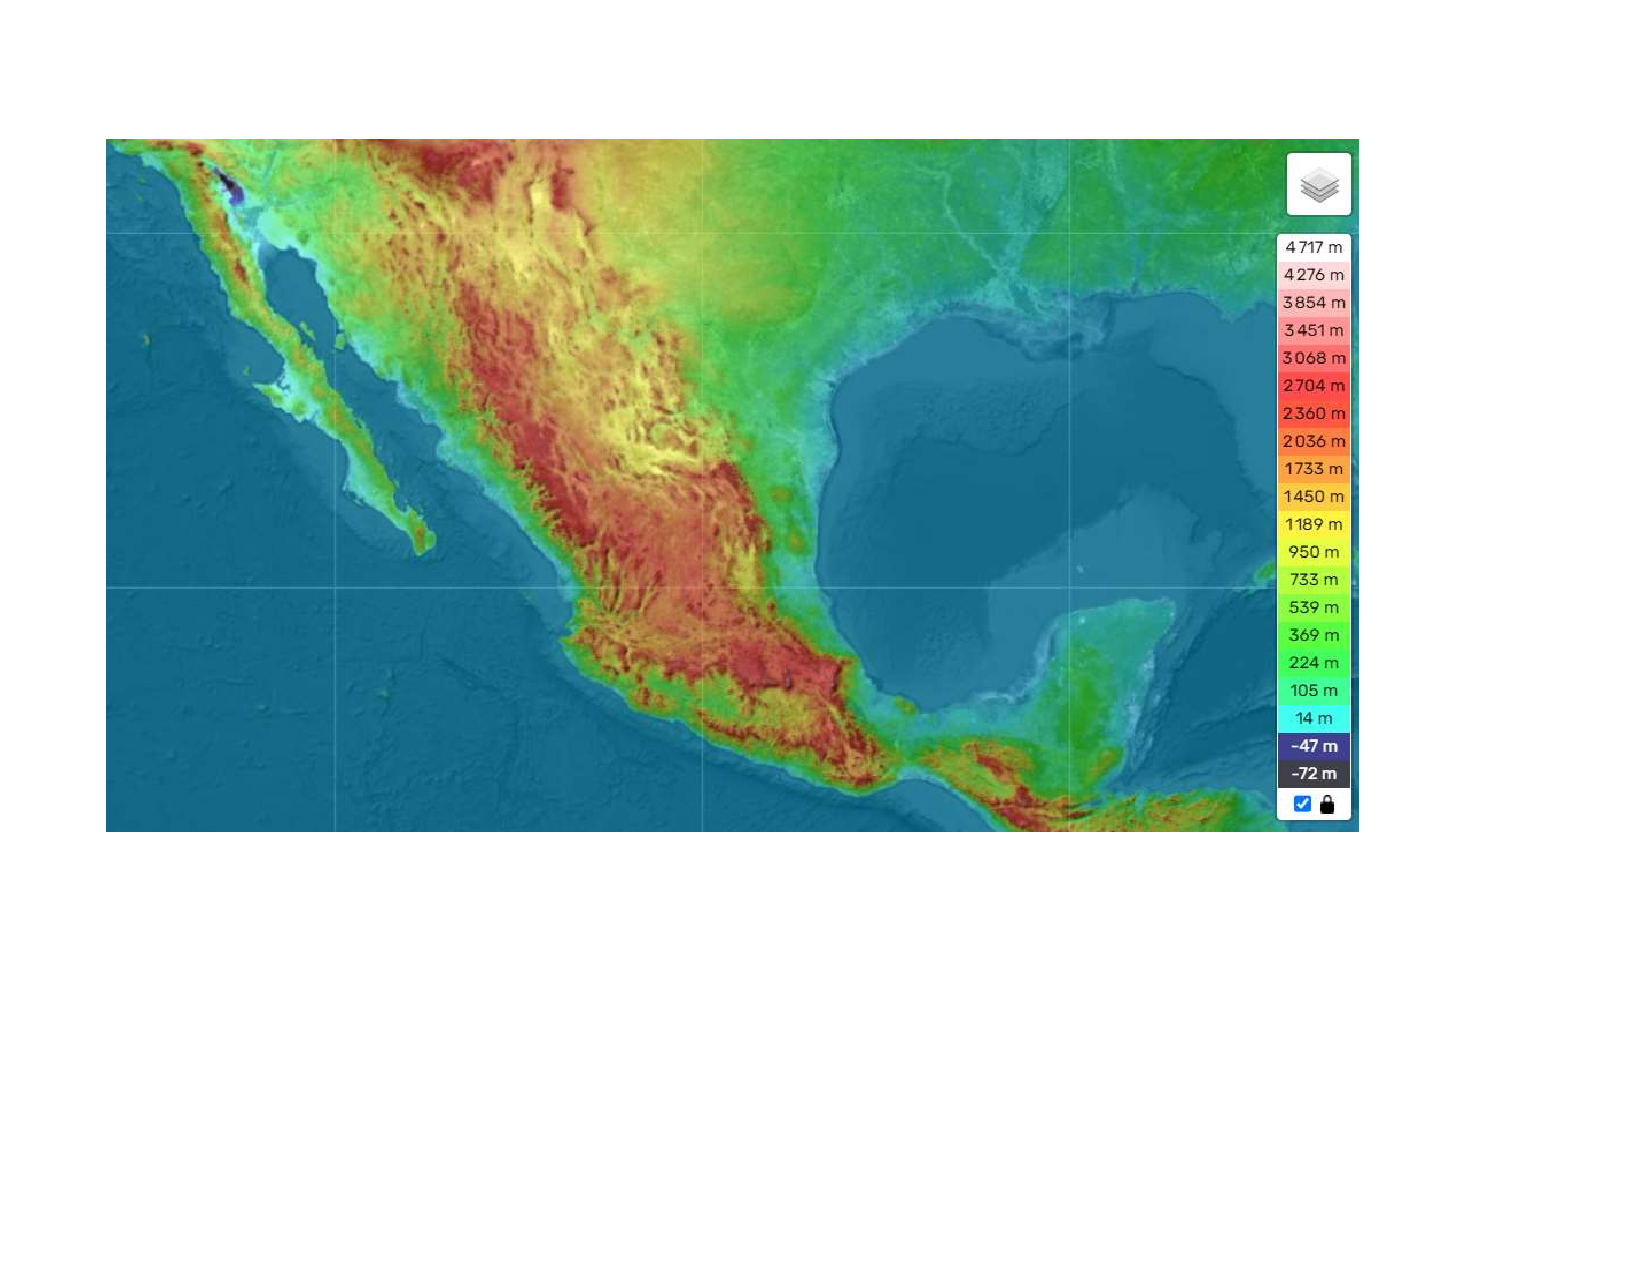
\includegraphics[scale=0.57]{Capitulo3/figs/altitud mexico_cropped.pdf}
\caption{Altitude of Mexico. de: mx.topographic-map.com}
\label{fig: Altitud de México}
\end{figure}

The Metropolitan Polytechnic University of Hidalgo (UPMH) is located in the municipality of Tolcayuca, state of Hidalgo, Mexico. $2,336 m$ on the level of the sea. Considering the roof of service at a height of $120 m$ a geometric altitude of $2,456 m$, and a cruise height of $90m$ for a geometric altitude of $2,426 m$. Ver Figura \ref{Definición de altitudes}.

\begin{figure}[!h]
\centering
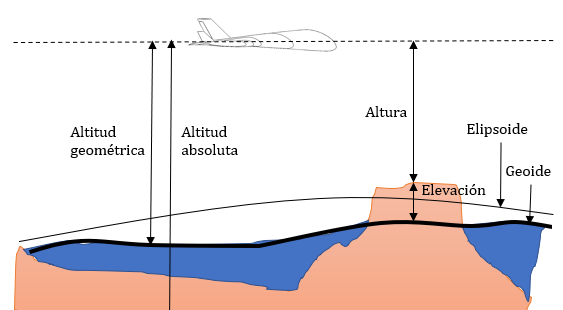
\includegraphics[scale=0.98]{Capitulo3/figs/3 4.png}
\caption{Definition of altitudes}
\label{Definición de altitudes}
\end{figure}

The properties of air (temperature, pressure and density) according to altitude and according to the International Standard Atmosphere are set below.\footnote{International Standard Atmosphere or ISA}

\medskip

\textbf{International Standard Atmosphere}

The Earth's atmosphere is a changing dynamic system whose behavior is described by pressure, density and temperature. 
%
These variables change with latitude, longitude, altitude, time of day, annual season, etc. 
%
To consider these variations and dependencies during the design of an aircraft or in the estimates of its performances is something impracticable and impracticable. 
%
The standard atmosphere objective is to provide a common reference to determine how the magnitudes that describe the behaviour of the air as a function of altitude change. 

Solution in the troposphere \cite{franchini2013}\\
We define the altitude in meters with the variable $z$. The distribution of temperature $T(z)$ is fixed by the standard atmosphere based on the experimental information collected, so the problem is reduced to the unknown pressure $p(z)$ and density $\rho(z)$. These equations are obtained from mathematical models that describe the physical and thermodynamic behavior of the air, which are: the equation of state of ideal gases and the equation of balance of forces.
%
The layer of the troposphere runs from the Earth's surface ($z=0km$) at sea level up to an altitude of $z=11km$. The temperature variation is expressed linearly depending on the altitude such that: $T(z)=T_0 + \lambda z$, where $T_0 = T(z=0)=288.15 K$ is the temperature at sea level and $\lambda = -6.5^{-3} \frac{K}{m}$ It's the temperature gradient. 

To calculate the temperature we use the equation:
\begin{equation}
\label{temperatura ISA}
    T = T_0 - \frac{1}{1000} 6.5 z
\end{equation}
The hydrostatic equation is defined as:
\begin{equation}
\label{hidrostática}
    dp = -\rho g dz
\end{equation}
The ideal gas equation is defined as:
\begin{equation}
\label{gas ideal}
    p = \rho R T 
\end{equation}
Dividing the equation \ref{hidrostática} between \ref{gas ideal} We have to:
\begin{equation}
    \frac{dp}{p}=-\frac{\rho g dz}{\rho R T} = - \frac{g}{RT}dz
\end{equation}
to calculate the pressure relative to the altitude, the temperature is assumed standard and the air is assumed as an ideal gas. \ref{temperatura ISA} the expression turns out to be:
\begin{equation}
    \frac{dp(z)}{p(z)}= - \frac{g}{R} \frac{dz}{T_0 + \lambda z}
\end{equation}
The solution of this problem is to obtain the variation of the pressure with respect to the altitude and, since it is in a differential operator, it is necessary to take the operator inverse to the differentiation, that is, the integration.
\begin{equation}
\label{integral ISA}
    \int_{p_0}^{p(z)} \frac{dp}{p} = \int_{0}^{z} - \frac{g}{R} \frac{dz}{T_0 + \lambda z}
\end{equation}
The lower limit of the integral is $z=0$ and the upper limit an arbitrar altitude $z$ less than or equal to $11,000 m$. Solving the integral \ref{integral ISA} We have to:
\begin{equation}
    ln (\frac{p(z)}{p_0})= - \frac{g}{R \lambda} ln (\frac{T_0 + \lambda z}{T_0})
\end{equation}
o bien
\begin{equation}
\label{presion ISA}
    p(z) = p_0 (1 + \frac{\lambda z}{T_0})^{(- \frac{g}{R \lambda})}
\end{equation}
where, $p_0 = 101,325 Pa$It's pressure at sea level. 

The variation of density relative to altitude is obtained by entering the equation \ref{presion ISA} in \ref{gas ideal} resulting in:
\begin{equation}
\label{densidad ISA}
    \rho(z) = \rho_0 (1 + \frac{\lambda z}{T_0})^{(- \frac{g}{R \lambda} - 1)}
\end{equation}
where, $\rho_0 = \frac{p_0}{R T_0} = 1.225 \frac{kg}{m^3}$, is the density of the air at sea level. 
\begin{figure}[!t]
\centering
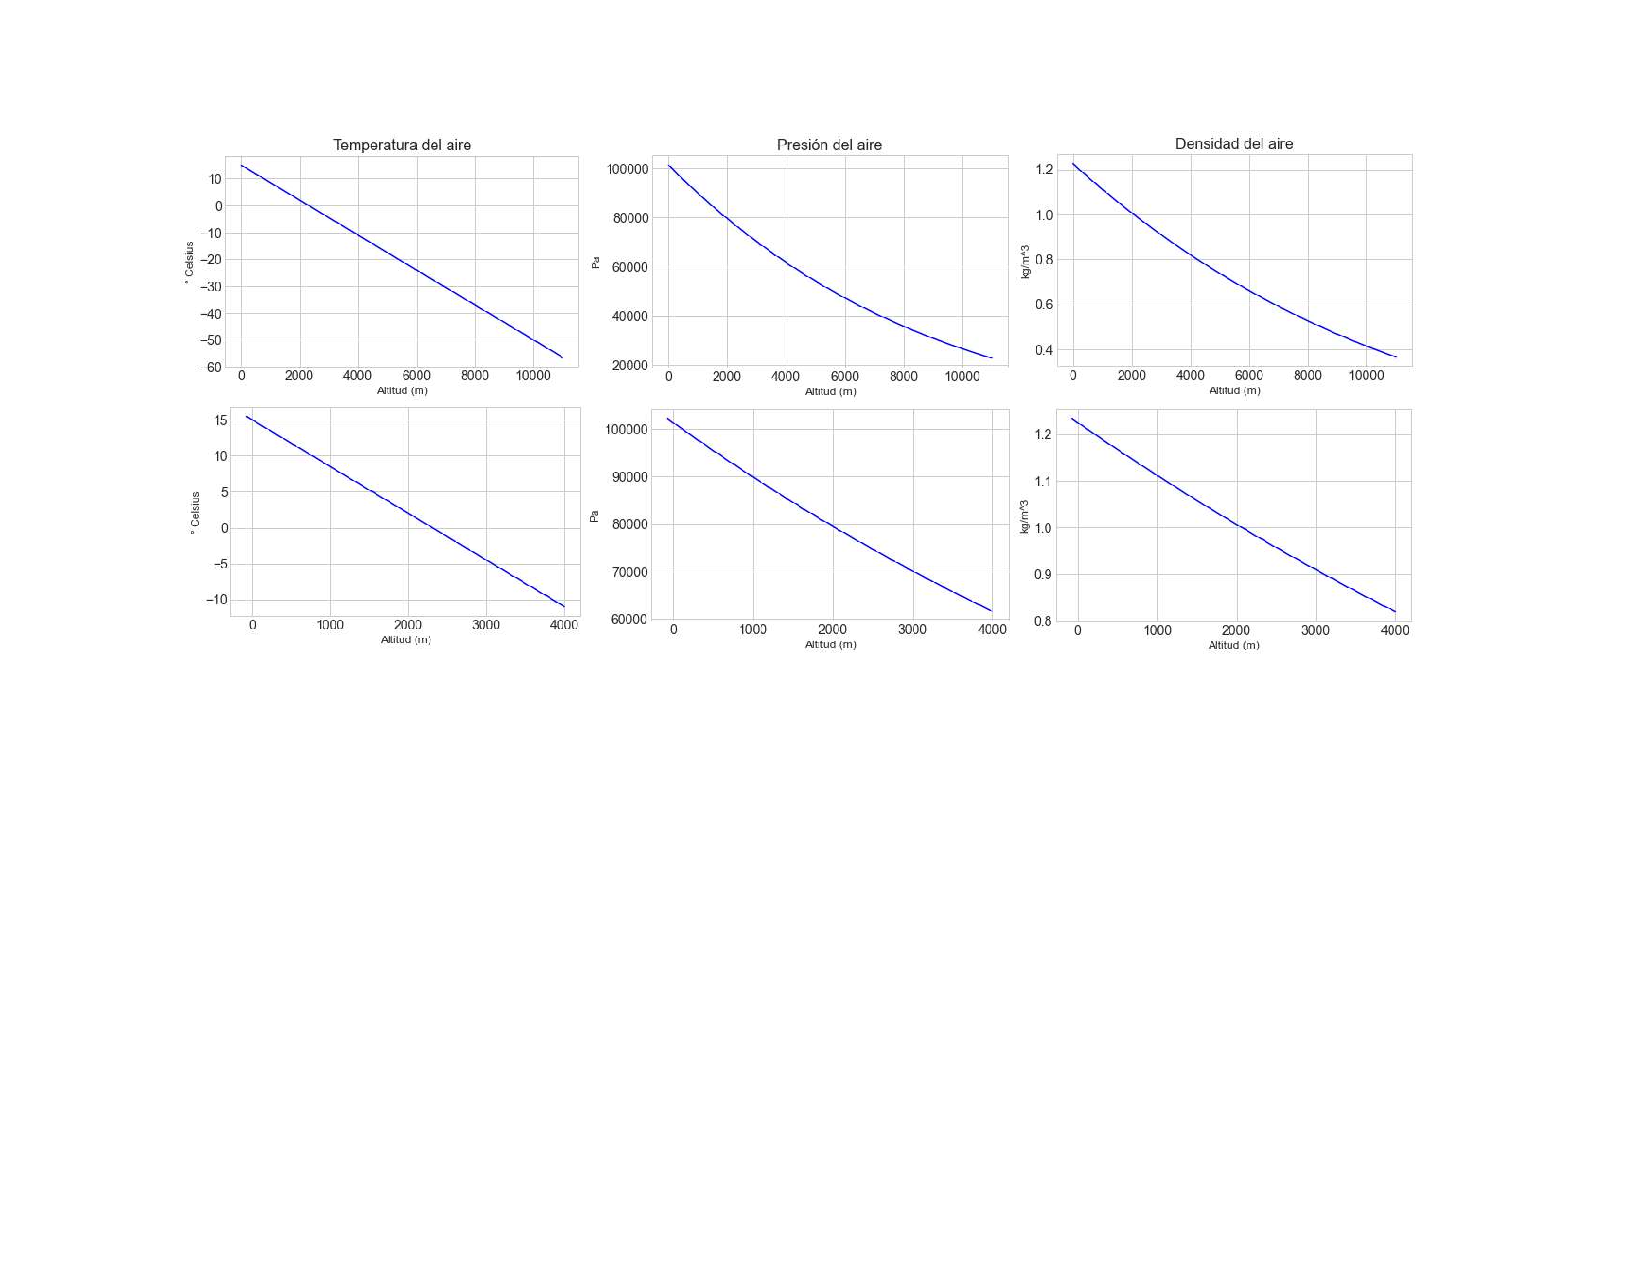
\includegraphics[scale=0.655]{Capitulo3/figs/aire en funcion de altitud_cropped.pdf}
\caption{Temperature, pressure and air density depending on altitude in the troposphere (1st row) and Mexican national territory (2nd row)}
\label{fig: Temperatura, Presión y Densidad del aire}
\end{figure}
\begin{table}[!h]
\caption{Air properties at the Metropolitan Polytechnic University of Hidalgo according to ISA}
\label{tab: Propiedades del aire en UPMH a $z=2,426m$ }
\centering
\begin{tabular}{ |p{9cm}|p{4cm}|  }
\hline
\multicolumn{2}{|c|}{Air properties in the UPMH for EHEKATL BWB}\\
\hline
Elevation in Tolcayuca, Hidalgo, Mexico & $2,336m$\\
Cruise altitude for EHEKATL BWB & $90m$\\
Geometric altitude cruise in UPMH &  $2,426m$ \\
Temperature at geometric altitude & $ -0.77 ^{\circ}C$\\
Pressure at geometric altitude & $ 75,367.8 Pa$\\
Density at geometric altitude & $0.9639 \frac{kg}{m^3}$\\
\hline
\end{tabular}
\end{table}

Figure \ref{fig: Temperatura, Presión y Densidad del aire} shows simulations of equations \ref{temperatura ISA}, \ref{presion ISA} and \ref{densidad ISA} for the altitude range of the troposphere (first row) and the altitude range of the Mexican national territory (second row). \ref{fig: Temperatura, Presión y Densidad del aire} shows the specific data according to the ISA for the location of the UPMH and the altitudes defined for the EHEKATL BWB flight mission.

%%%%%%%%%%%%%%%%%%%%%%%%%%%%%%%%%%%%%%%%%%%%%%%%
\section{Aerodynamic design}

The considerations in the aerodynamic design of a wing-integrated aircraft are similar to those of a wing-flyer, see Table \ref{tab: Objetivos Diseño Aerodinámico EHEKATL BWB}We can analyze EHEKATL BWB as a \textbf{Unmanned Air System} consisting of subsystems consisting of components and parts thereof. 
\begin{table}[!h]
\caption{Aims of the aerodynamic design EHEKATL BWB}
\label{tab: Objetivos Diseño Aerodinámico EHEKATL BWB}
\centering
\begin{tabular}{ |p{4cm}|p{9cm}|  }
\hline
\multicolumn{2}{|c|}{\textbf{Aims of the aerodynamic design EHEKATL BWB}}\\
\hline
\textbf{Generales} & Performance, stability and control.\\
\hline
\textbf{Optimization} & Maximize support and minimize drag. \\
\hline
\textbf{Static stability} & Negative pending at the time of heading and rolling; and positive slope at the time of yaw. \\
\hline
\textbf{Design variables} & Alar profile, span and length, reference area, arrow, incidence, diedro, vertical stabilizers, tip fins, aerodynamic control surfaces and centre of gravity. \\
\hline
\textbf{Environmental variables} & Angle of attack and skid; speed, temperature, pressure, density and viscosity of air flow; number of Reynolds and Mach. \\
\hline
\end{tabular}
\end{table}
The subsystems defined for EHEKATL BWB are: support, propulsion, avionics, structures and energy.\\
The \textbf{Support subsystem} The components of the support subsystem of EHEKATL BWB involve consideration of the type of wing profile and geometry for the central body, outer wing, direction stabilizers and fins at the wing tip. \\
The \textbf{Propulsion subsystem} on wing-integrated aircraft offers a wide range of possibilities. As stated in the background section and visually in the Figure \ref{fig: propulsion distribuida}, we can locate the engines under the outer wing or above the central body, implement propulsion systems of intake of the boundary layer and/or distributed propulsion systems, as well as implement deflective nozzles that allow vector thrust control. For the aircraft EHEKATL BWB we will establish two ductofan engines above the central body. In this first version only the thrust of the engines is considered without the generation of moments of the TVC. \\
The \textbf{avionics subsystem} is essential to ensure full wing flights in view of their unstable nature.
%
The main inputs to the flight controller are the gyroscope, the accelerometer and the barometer; as well as GPS and telemetry receivers that allow real-time information to be obtained at the ground station. At the controller output we have: actuators (servos-mechanisms) that allow the movement of the ACS, electronic speed controllers that allow to regulate the acceleration/deceleration of the engines, and the engines themselves that give the push force to reach speeds that allow our aircraft to sustain itself and generate maneuvers for its navigation. 
%
the graphics card and camera are considered the payload of EHEKATL BWB.

The \textbf{Energy subsystem} is a focal point on a wing-integrated aircraft since we are looking for a zero emissions or low emissions aircraft (depending on application).
%
In the geometry of BWB we can implement subsystems of electric energy, fossil fuel, bio-fuels, hydrogen cells or hybrids. This thanks to the fact that BWB has greater central capacity than TAW aircraft, which allows the deployment of hydrogen cells in the central body. TAW models place their fuel tanks in the wing, which for applications of hydrogen cells would be complex to implement.
%
In this version of EHEKATL BWB we will assume electric batteries as an energy subsystem for simplicity but meeting the zero emissions target.

The \textbf{subsistema estructural} of an unmanned aerial vehicle is usually made of wood, composite materials among which stand out the fibers of glass and carbon, also some alloys or metals. The detailed design is beyond the scope of this thesis project. \ref{superficie alar y potencia requerida} entitled wing surface and required power, we calculate the empty weight based on a linear regression of aircraft of similar characteristics in dimension, relating to the weight and obtaining an estimate for this subsystem, important condition for the rest of design calculations. 


In this thesis work for the aerodynamic design of EHEKATL BWB is made use of XFLR5 and X-PLANE software. The latter in its Airfoil Maker extensions for the design of wing profiles and Plane Maker for the design of the EHEKATL BWB aircraft. 

\bigskip
%%%%%%%%%%%%%%%%%%%%%%%%%%%%%%%%%%%%%%%%
\subsection{Selection of Alalar Profiles in XFLR5}
The aerodynamic profile or wing profile is the geometry of the cross section in a lateral view of the supporting surface or wing. \textit{reflex} are non-symmetric profiles that have a medium comba line with double slight curvature in the form of \textit{S}, which is why they are also known as "S" profiles, normally used in wings-flying and integrated wings. \cite{gatovolante2015}, the most significant feature of the reflex profiles is that they are profiles with positive stability, that is to say their moment coefficient is always positive except and very occasionally at very high attack angles, this results in that the wing with this type of profile flies in balance without the need for horizontal stabilizers, so its widespread use is in delta type wings, wing-flyers and integrated wings. 
%
Under these conditions the centre of gravity of the model shall be located in the direction of the resulting aerodynamics that always passes through the pressure centre that is determined by the moment coefficient and supporting coefficient. 
%
The theoretical point of the wing where the lift is considered applied is called a centre of pressure. For theoretical purposes, although the pressure acts on the whole profile, it is considered that all the lift is exerted on a point in the line of the rope (resulting). The position of the pressure centre is usually given in $\%$ of the wing rope from the edge of attack. 
%
In the case of self-stable profiles it places the center point between 20 and 25 $\%$ of the aerodynamic mid-string.
%
If an external disturbance alters the position of the wing, causing this spike, its center of pressure, to move forward away from the center of gravity, which immediately causes a moment of encabritation (above) that tends to the wing regain its initial balance. 
%
The main drawback of these types of profiles is that they have relatively low lift coefficients while their drag coefficients are high. 
%
Visually, aircraft with these types of profiles appear to have the trailing edge and the ailerons slightly oriented upwards. This geometry is responsible for generating stability at the moment of pitching. If we used a symmetrical profile instead of a profile \textit{reflex} In the design of a wing-integrated we would need a wide bending capacity of the elevators and a complex control system for a stable flight, which generates a constant consumption of energy given the continuous deflection of the effectors, and therefore would decrease the aerodynamic performance of the aircraft. 

\begin{table}[!h]
\caption{Aerodynamic profiles for concept generation}
\label{tab: Perfiles aerodinámicos EHEKATL BWB}
\centering
\begin{tabular}{ |p{14cm}|  }
\hline
\multicolumn{1}{|c|}{\textbf{Aerodynamic profiles for the generation of concepts}}\\
\hline
LA2573A, IU1720 , FAUVEL 14, MARSKE PIONNER IA, MARSKE XM 1D\\
MH78, MH80, MH91, MH92, MH93\\
NACA 0009, WORTMANN FX 71 120\\
\hline
\end{tabular}
\end{table}
\begin{figure}[!h]
\centering
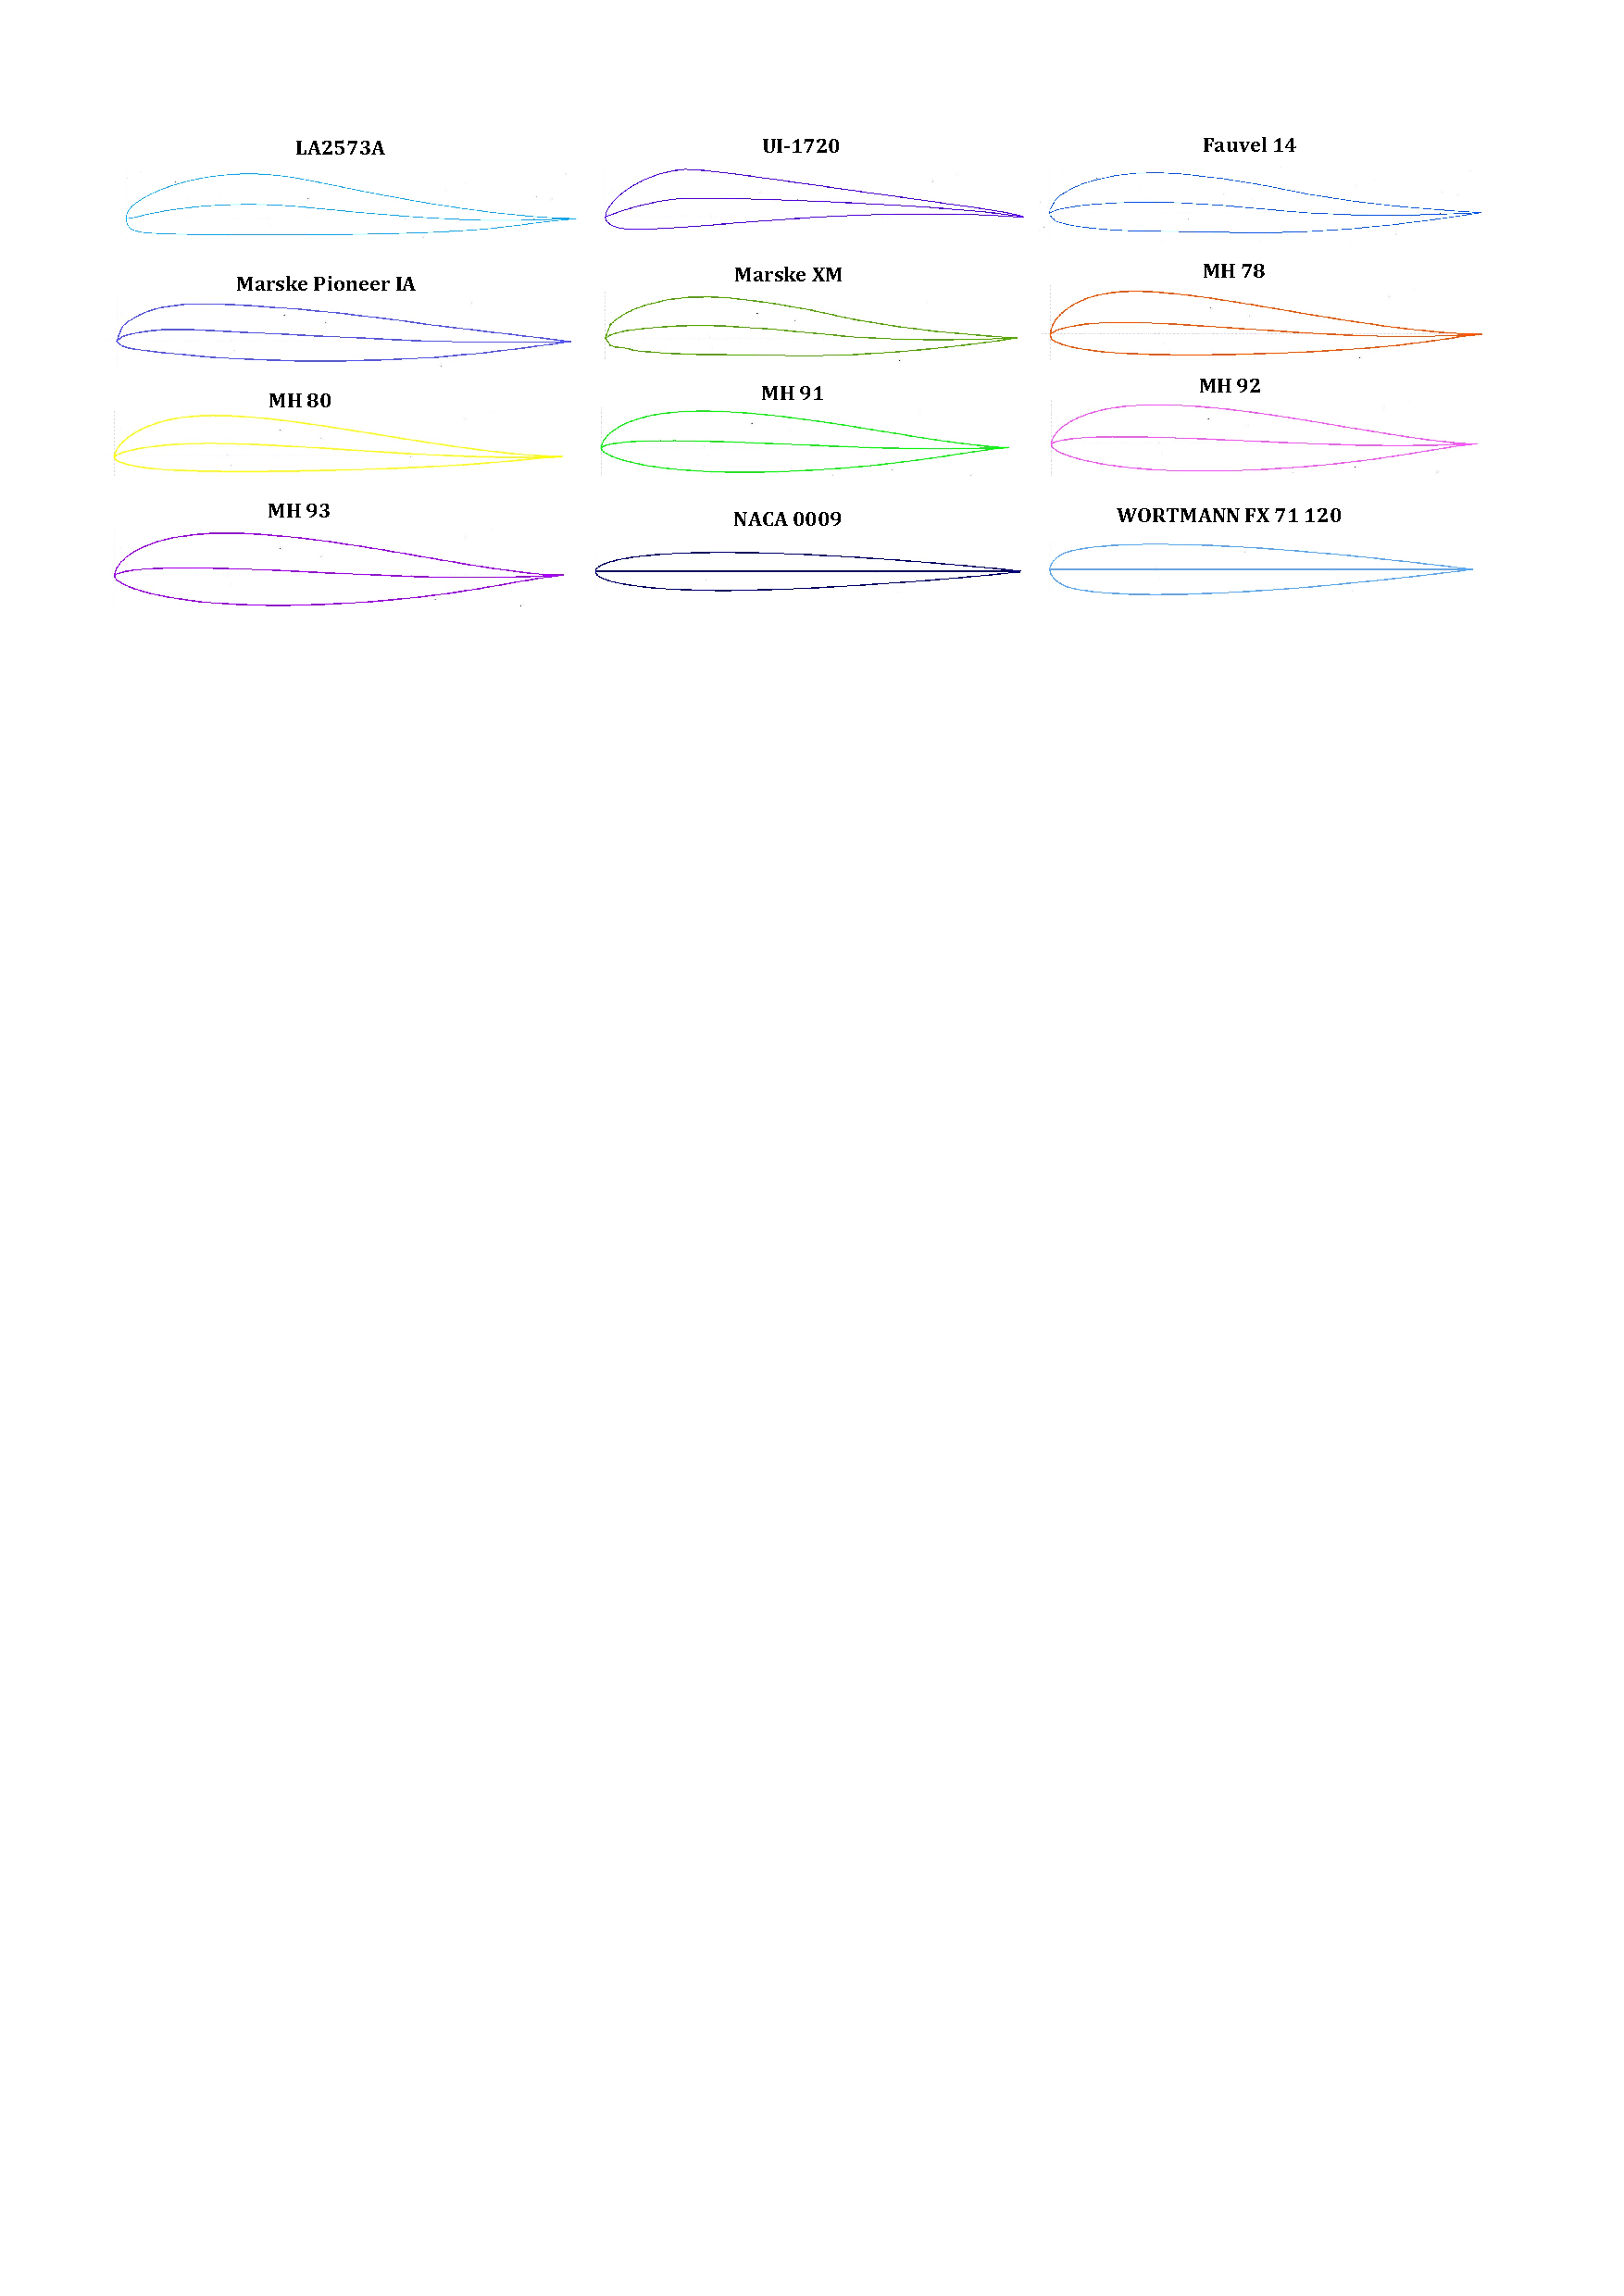
\includegraphics[scale=0.50]{Capitulo3/figs/perfiles aerodinamicos cropped.pdf}
\caption{Aerodynamic profiles}
\label{perfiles aerodinamicos}
\end{figure}

The following profiles were selected for EHEKATL BWB.
\begin{itemize}
    \item \textbf{MH80} central body
    \item \textbf{MH78} in the outer wing
    \item \textbf{NACA 0009} in vertical stabilisers
\end{itemize}

To compare the performance of the profiles selected for EHEKALT BWB, the twelve aerodynamic profiles of the Table were selected \ref{tab: Perfiles aerodinámicos EHEKATL BWB}. 
%
In the Figure \ref{perfiles aerodinamicos} the images of the aerodynamic profiles of the Table are shown \ref{tab: Perfiles aerodinámicos EHEKATL BWB}. Since the profiles selected for EHEKATL BWB are the profiles MH78 (yellow), MH80 (orange) and NACA 0009 (grey) it is recommended to pay attention to the performance of these profiles in the results of the aerodynamic analysis of the Figures \ref{perfiles aerodinamicos vstall} and \ref{perfiles aerodinamicos vmax} where a rope of 1m is considered in a speed regime of 19$m/s$ and 35$m/s$ four graphs are shown in the aerodynamic simulations: lift coefficient $C_L$ depending on the angle of attack $\alpha$, drag coefficient $C_D$ as a function of $\alpha$, polar $C_L / C_D$ as a function of $\alpha$ and pitching-moment coefficient $C_m$ as a function of $\alpha$.
%
Three of the above profiles are not reflex profiles. We are talking about UI-1720, NACA 0009 and WORTMANN FX 71 120. 
%
The aerodynamic profile UI-1720, was selected for its high lift coefficient and low drag coefficient. However, since the comba of the trailing edge does not meet the criterion of reflex profiles, the moment coefficient of pitch does not meet the stability requirements, indispensable in the design of wing-flyers and integrated wings. This profile is considered to contrast the aerodynamic efficiency of the rest of the reflex profiles.
%
In the case of NACA 0009 and WORTMANN FX 71 120 profiles, both are symmetrical profiles. The objective of vertical stabilisers is to provide lateral-directional stability to the air vehicle, for this reason symmetrical profiles are selected for these stabilizers that carry steering rudders.
%
In the Figures \ref{perfiles aerodinamicos vstall} and \ref{perfiles aerodinamicos vmax} the representative color of each profile is shown on the right. Each profile has its name and a description similar to \textit{T1 Re0.19 M0.06 N9.0}, where \textit{T1} is the type of simulation (continuous lines with respect to $\alpha$), $Re0.19$ for the Reynolds number which in this case is 0.19, $M0.06$ for a Mach of 0.06 and $N9.0$ representa $N_{crit}$ equal to 9.0 for a laminar flow. 

\begin{figure}[!h]
\centering
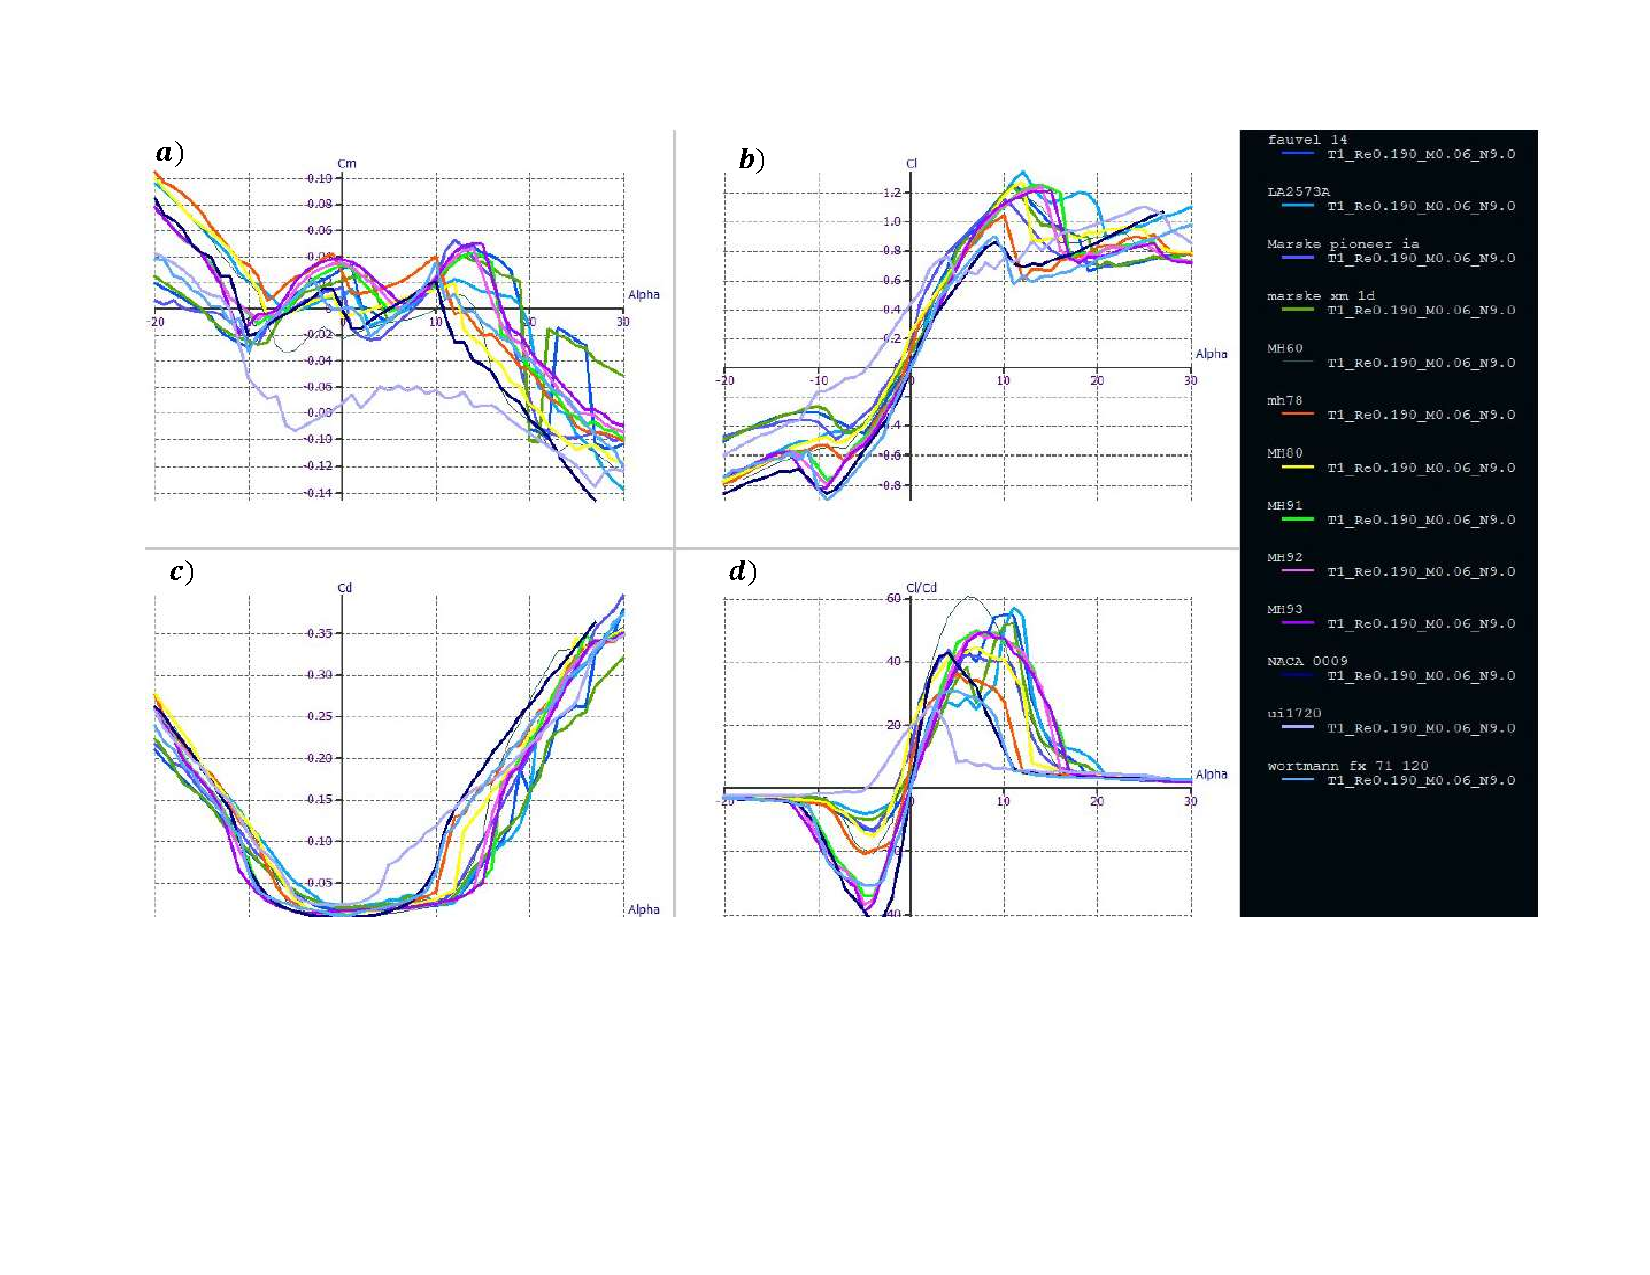
\includegraphics[scale=0.58]{Capitulo3/figs/perfiles 19ms_cropped.pdf}
\caption{Analysis of Aerodynamic Profiles.Loss Speed: $19 m/s$,Re: $1.9^6$, Mach: $0.055$}
\label{perfiles aerodinamicos vstall}
\end{figure}


\textbf{Analysis of Profile Results at 19m/s.} Figure \ref{perfiles aerodinamicos vstall} shows the aerodynamic analysis of the profiles at a speed of 19m/s. According to graph a) it is observed that the profiles MH80 and MH78 are kept close to zero but with a positive margin in $C_m$. The MH78 profile maintains a positive margin across the entire range of $\alpha$ of interest, ranging from -10$^\circ$ up to 10$^\circ$, while MH80 has some negative values in this range. Both profiles meet the stability criterion for pitching, but MH78 demonstrates better performance in this category. In graph b) it is observed that the MH80 profile is one of the profiles with the best $C_{L_{max}}$, with a value of 1.25 for a $\alpha$ of 14$^\circ$. The MH78 profile in place has a $C_{L_{max}}$ of 1.03 with a $\alpha$ of 10$^\circ$. In graph (c) MH78 and MH80 profiles show high values in $C_D$ for the other profiles for this speed regime, for this reason in graph d) the MH78 profile shows an efficiency of 37 with respect to $C_L/C_D$, while MH80 shows an efficiency of 45. While they are acceptable values, compared to the rest of profiles an intermediate efficiency is shown for this speed regime.  

\begin{figure}[!h]
\centering
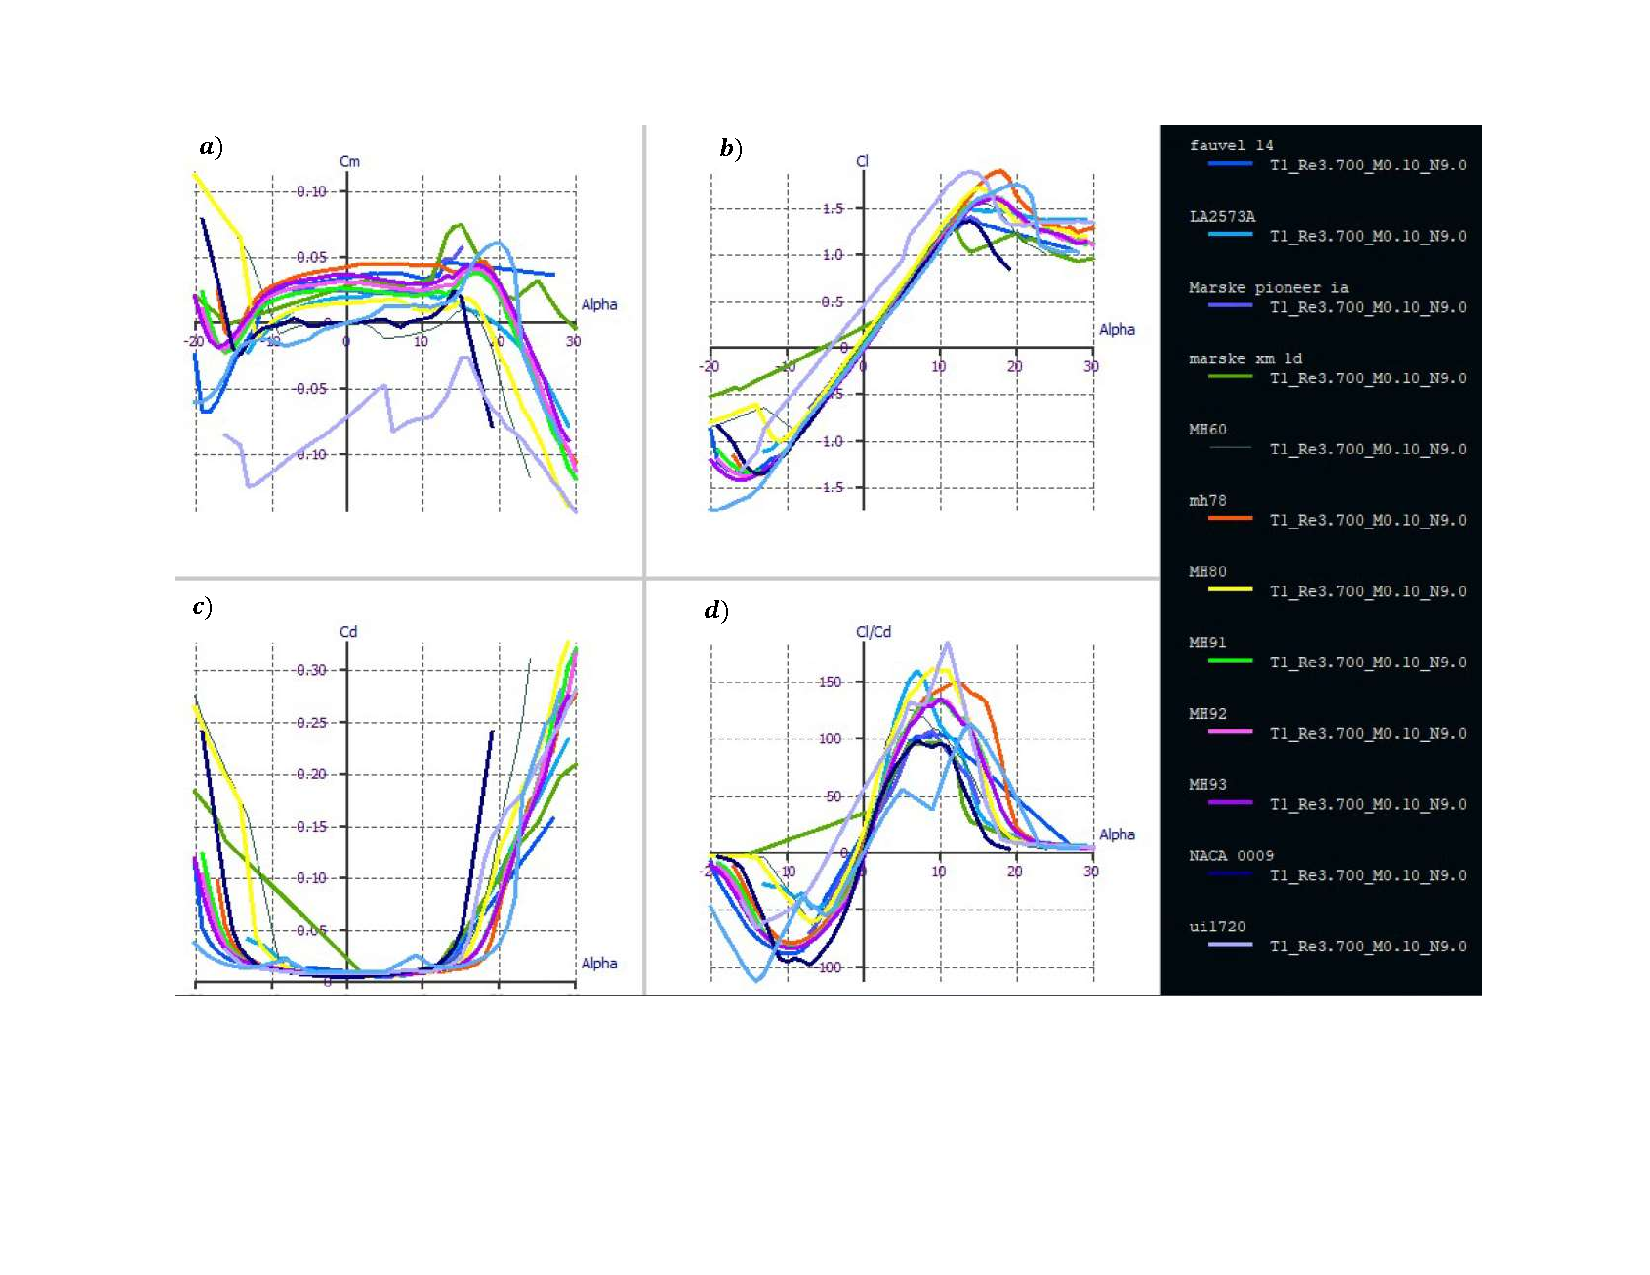
\includegraphics[scale=0.6]{Capitulo3/figs/perfiles 35ms_cropped.pdf}
\caption{Analysis of Aerodynamic Profiles.Maximum Speed: $35 m/s$,Re: $3.7^6$, Mach: $0.1$}
\label{perfiles aerodinamicos vmax}
\end{figure}
\textbf{Analysis of Profile Results at 35m/s.} Figure \ref{perfiles aerodinamicos vmax} shows the aerodynamic analysis of the profiles at a speed of 35m/s. $C_m$ more stable compared to speed of 19$m/s$. Now, the MH80 profile has all its positive values and close to zero in the range of $\alpha$ of -10$^\circ$ to 10$^\circ$On the other hand, MH78 maintains its positive values, above the values of MH80 but less than 0.05, which are also considered close to zero. In this speed regime we have better stability for the moment of pitching than in the previous regime of 19$m/s$ in both profiles, but even MH78 offers better stability for the moment of pitching. In graph b) it is shown as now are the profiles MH78 and MH80 with the best performance in $C_L$ after the UI-1720 profile. In support criteria, we are interested in the values of $C_L$ from $\alpha$ equal to 0$^\circ$ up to the value of $\alpha$ for $C_{L_{max}}$. In this approach, MH78 offers a $C_{L_{max}}$ around 2, being above the UI-1720 profile. On the other hand, MH80 offers good performance with a $C_{L_{max}}$ Although the UI-1720 profile considered to be high support shows values above both profiles (MH78 and MH80), in terms of $C_{L_{max}}$, MH78 achieved a higher coefficient and Mh80 is just below. In graph c) we see a better performance in $C_D$ for both profiles in this speed regime than the previous one of 19$m/s$The MH78 profile proves to be one of the profiles with the lowest drag coefficient, while MH80 also decreased these values notably. In graph d) it is MH78 and MH80 that offer the best performance along with UI-1720 and LA2573A. MH80 shows slightly better performance than MH78, with values $C_L/C_D$ over 150, while MH78 barely reaches 150. This because MH80 had a $C_L$ above MH78 in a range $\alpha$ of 0$^\circ$ 12$^\circ$, however the MH78 has better ability to collapse with higher values in $C_L$ after $C_{L_{max}}$.  

The selection criteria for the MH78 and MH80 profiles were due to their good aerodynamic performance in $C_L$, $C_D$ and $C_L/C_D$, which exceeds most profiles as the speed regime increases. The MH80 profile is selected for the central body, since this section of the aircraft has the largest reference area, and MH80 offers a greater reason $C_L/C_D$ from a $\alpha$ of 0$^\circ$ up to 12$^\circ$As a result, the MH78 profile is selected for the outer wing section since MH78 offers better qualities for pitch stability and collapse capacity.

\medskip

%%%%%%%%%%%%%%%%%%%%%%%%%%%%%%%%%%%%%%%%%%%
\subsection{Design of Alalar Profiles in Airfoil Maker}
Airfoil Maker is a tool within the X-PLANE simulator to design or modify any wing profile that we are interested in implementing in an aircraft within the simulation environment of X-PLANE. The aerodynamic profile design in Airfoil Maker is based on the coefficients of support, drag and pitching time. Airfoil Maker allows to implement the behavior of wing profiles for a specific number of Reynolds, and as many Reynolds numbers can be implemented as desired or necessary. X-PLANE 11 software has a list of available wing profiles (30 elements), including the NACA 0009 profile. In the Figure \ref{Perfiles alares MH80 y MH78 en X-PLANE} The graphical design based on nodes is observed to reach the geometry of the profiles MH78 and MH80. These geometries are of visual reference and do not influence the aerodynamic behavior of the profiles. 
\begin{figure}[!h]
    \centering
    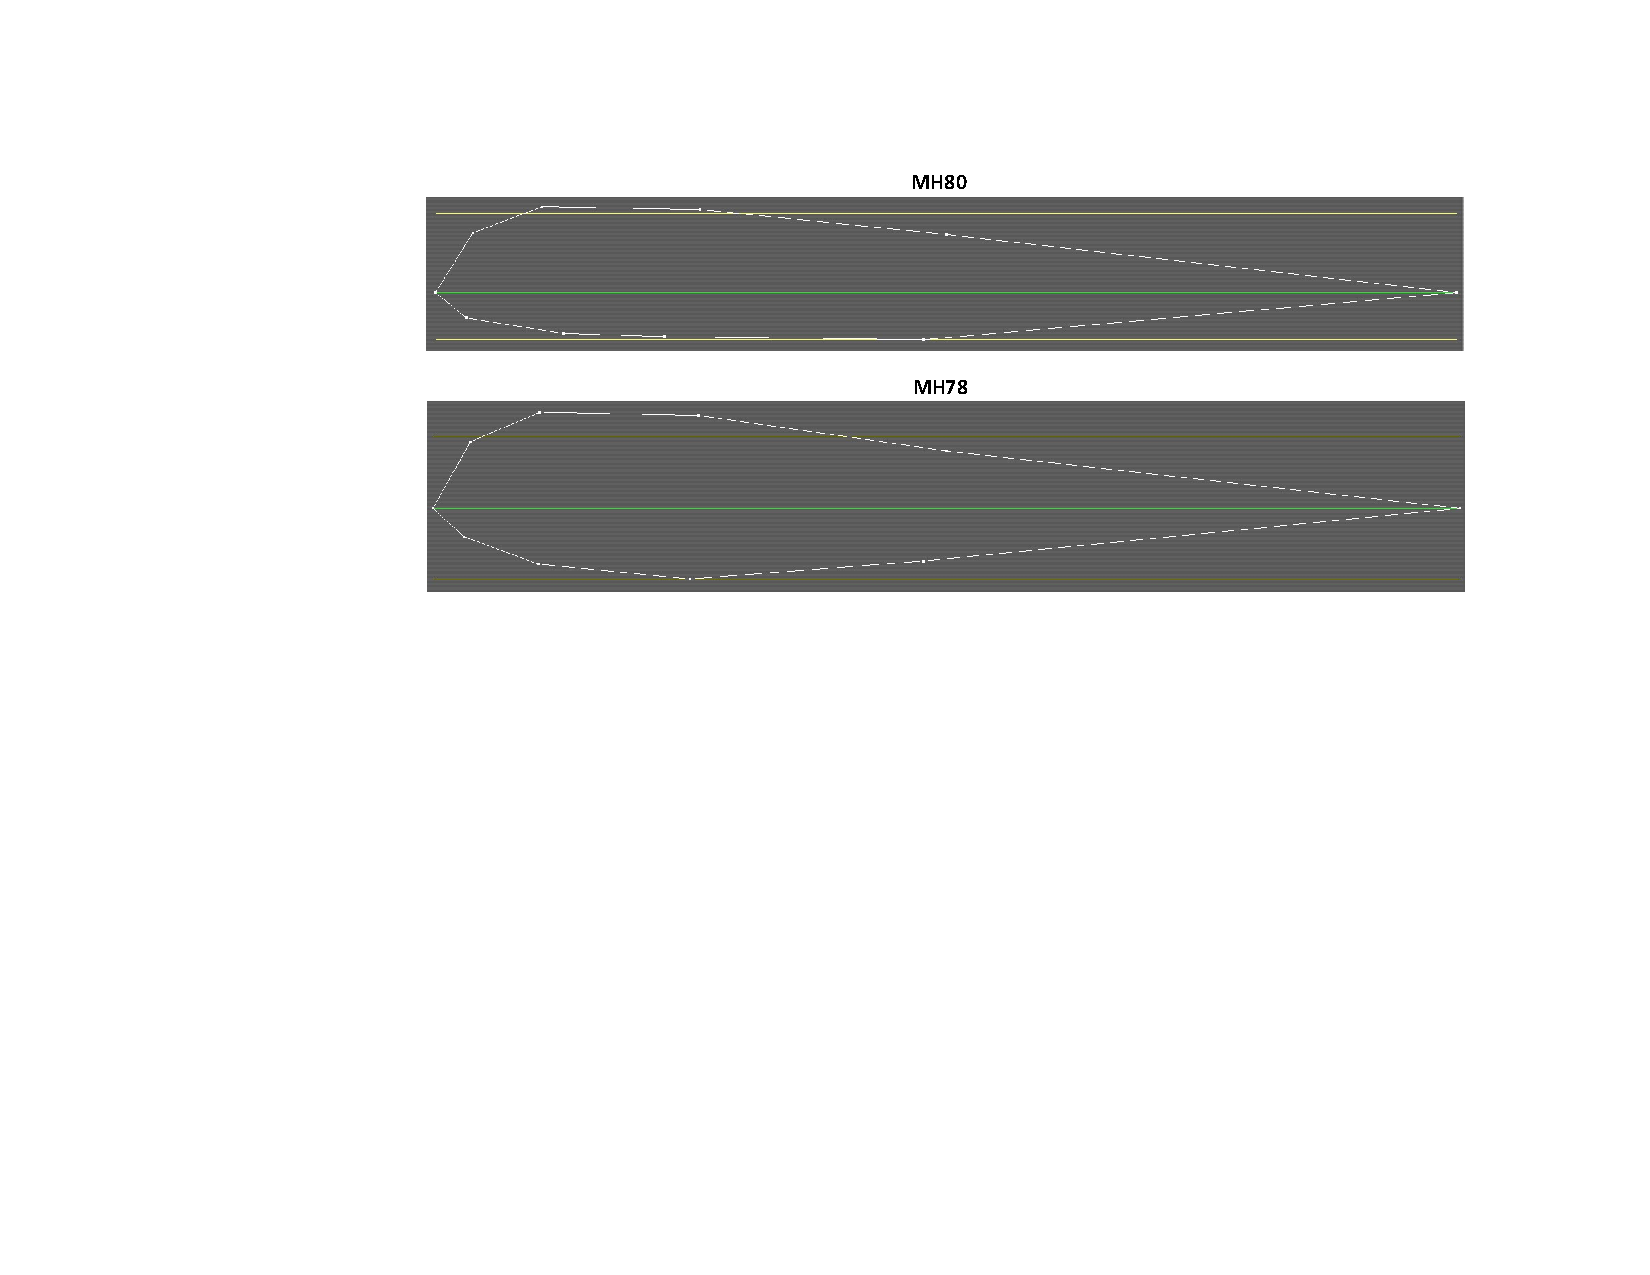
\includegraphics[scale=0.63]{Capitulo3/figs/perfiles xplane_cropped.pdf}
    \caption{Geomtry of MH80 and MH78 wing profiles in Airfoil Maker}
    \label{Perfiles alares MH80 y MH78 en X-PLANE}
\end{figure}
The aerodynamic simulations of the Figure are used to parameterize the MH78 and MH80 profiles \ref{Desempeño de perfiles réflex MH-78 (azul) y MH-80(rojo)},
\begin{figure}[!h]
    \centering
    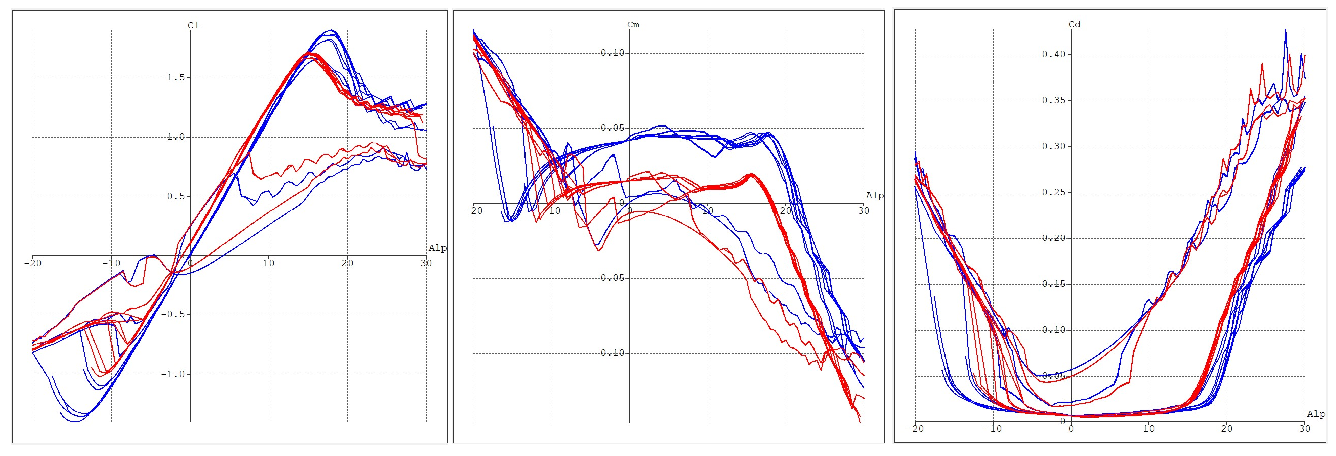
\includegraphics[scale=0.62]{Capitulo3/figs/mh78 y mh80.pdf}
    \caption{Reflex profile performance MH78 (blue) and MH80(red)}
    \label{Desempeño de perfiles réflex MH-78 (azul) y MH-80(rojo)}
\end{figure}
where simulations of the profiles MH78 and MH80 are shown for Reynolds numbers from $10,000$, $100,000$, $1,000,000$ and $4,000,000$.   
%
Low number of Reynolds ($10,000$ and $100,000$) show a behavior of MH78 and MH80 with low values of $C_L$ (less than 1) and a behavior with quite a few nonlinearities. $C_m$ negative and positive oscillator values around zero are shown (not complying with the pitch stability criterion), and the higher values in $C_D$ (from 0.1 to 0.4) also with a behavior that shows quite a few nonlinearities. As the number of Reynolds increases in the order of $1,000,000$ a $4,000,000$ better defined functions with a lower degree of non-linearities can be observed. $C_L$ a well-defined slope is shown as well as the $C_{L_{max}}$ (with values above 1.5). $C_m$ both profiles retain positive values in the range of $\alpha$ close to zero (which ensures pitch stability) within the interest range of -10$^\circ$ to 10$^\circ$, and the $C_D$ is kept low (from 0.005 to 0.15) in a range of $\alpha$ of -20$^\circ$ 20$^\circ$.

Two Reynolds numbers are selected for the design of the MH78 and MH80 profiles in Airfoil Maker: $1,000,000$ and $4,000,000$. In the Figure \ref{param mh78 airfoil maker} the configuration of the parameterization of the profiles MH78 and MH80 is observed in Airfoil Maker for the $1e6$ and $4e6$ respectively. 
\begin{figure}[!h]
    \centering
    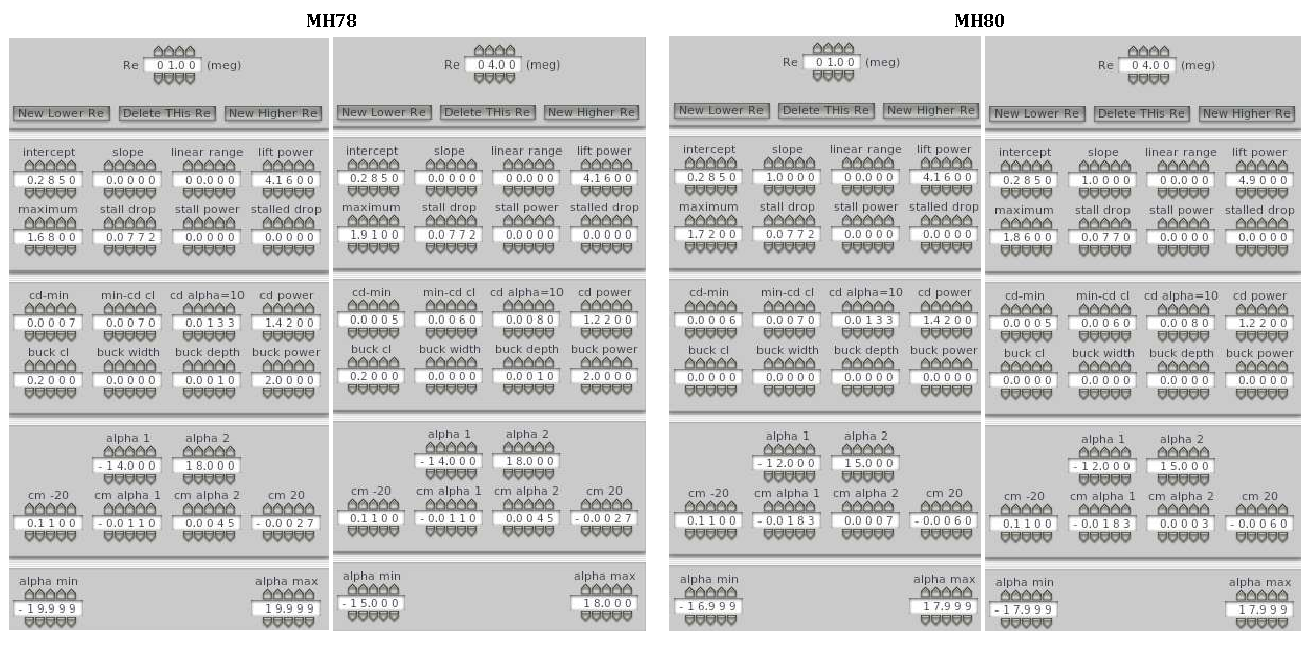
\includegraphics[scale=0.63]{Capitulo3/figs/am mh78 80.pdf}
    \caption{MH78 and MH80 Parametrization at Airfoil Maker}
    \label{param mh78 airfoil maker}
\end{figure}
Parametrization of the profiles in Airfoil Maker is done according to the four blocks that are seen in the Figure \ref{param mh78 airfoil maker}. In the first block, the function of $C_L$ concerning $\alpha$. In the second block, the function of $C_D$ concerning $\alpha$. In the third block, the function of $C_m$ concerning $\alpha$. Finally, in the fourth block, the values of $\alpha$ min and $\alpha$ for the configurations of $C_L$,$C_D$ and $C_m$. 

In the Figure \ref{MH78 en Airfoil Maker} results are observed in terms of profiles MH78 and MH80 in Airfoil Maker according to the parameterization of the Figure \ref{param mh78 airfoil maker}. The values of $C_L$, in red the values of $C_D$ and in yellow the values of $C_m$. Stronger or better defined lines correspond to the functions with $4e6$, while the fainter or less defined correspond to the functions with $1e6$.  
%
One particular feature of Airfoil Maker is that it does not restrict the visualization of aerodynamic functions in a normal range of attack angle between -20 and 30, instead, it shows the $360$ In spite of this the parameterization of our profiles was based only on a maximum range of $\alpha$ of -20$^\circ$ 20$^\circ$.
\begin{figure}[!h]
    \centering
    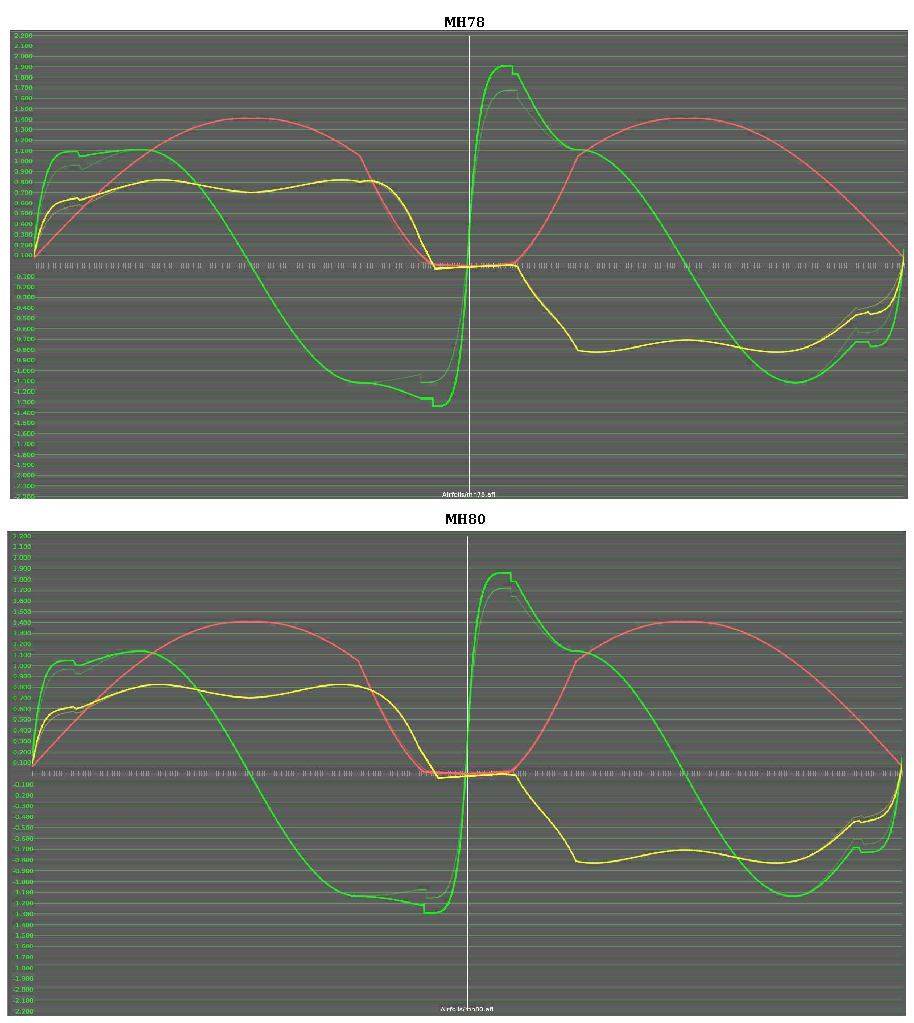
\includegraphics[scale=0.75]{Capitulo3/figs/mh78 80 per.pdf}
    \caption{Aerodynamic performance of MH78 and MH80 an Airfoil Maker}
    \label{MH78 en Airfoil Maker}
\end{figure}



%tenemos el intercepto (\textit{intercept}), que refiere al valor de $C_L$ cuando $\alpha$ es cero. La pendiente (\textit{slope}) ajusta la inclinación de la función en un su rango lineal rango que va de -15$^\circ$ a 15$^\circ$ aproximadamente. 
%Con el rango lineal (\textit{linear range}) podemos ajustar este rango de -15$^\circ$ a 15$^\circ$ para incrementarlo o reducirlo. La potencia de lift (\textit{lift power}) maneja la curva de los valores próximos a $C_{L_{max}}$, entre mayor potencia, se observa una curva más amplica alrededor de $C_{L_{max}}$. Máximo (\textit{maximum}) representa el valor de  $C_{L_{max}}$. La bajada de desplome (\textit{stall drop}) ajusta la forma de la función $C_L$ en el descenso después del $C_{L_{max}}$. La potencia de desplome (\textit{stall power}) ajusta que tanto va a bajar la función de $C_L$ después de $C_{L_{max}}$.%
%La bajada de desplome (\textit{stalled drop}) determinar la inclinación de la curva después de la bajada de desplome. 

%%%%%%%%%
\subsection{Aerodynamic Analysis with XFLR5}
Now, the main variables of aerodynamic design in BWB aircraft and their impact on EHEKATL BWB are defined. \ref{EHEKATL BWB G-33 Vista Isometrica} show the geometric design of the EHEKATL BWB aircraft in isometrics.    

\begin{figure}[!h]
    \centering
    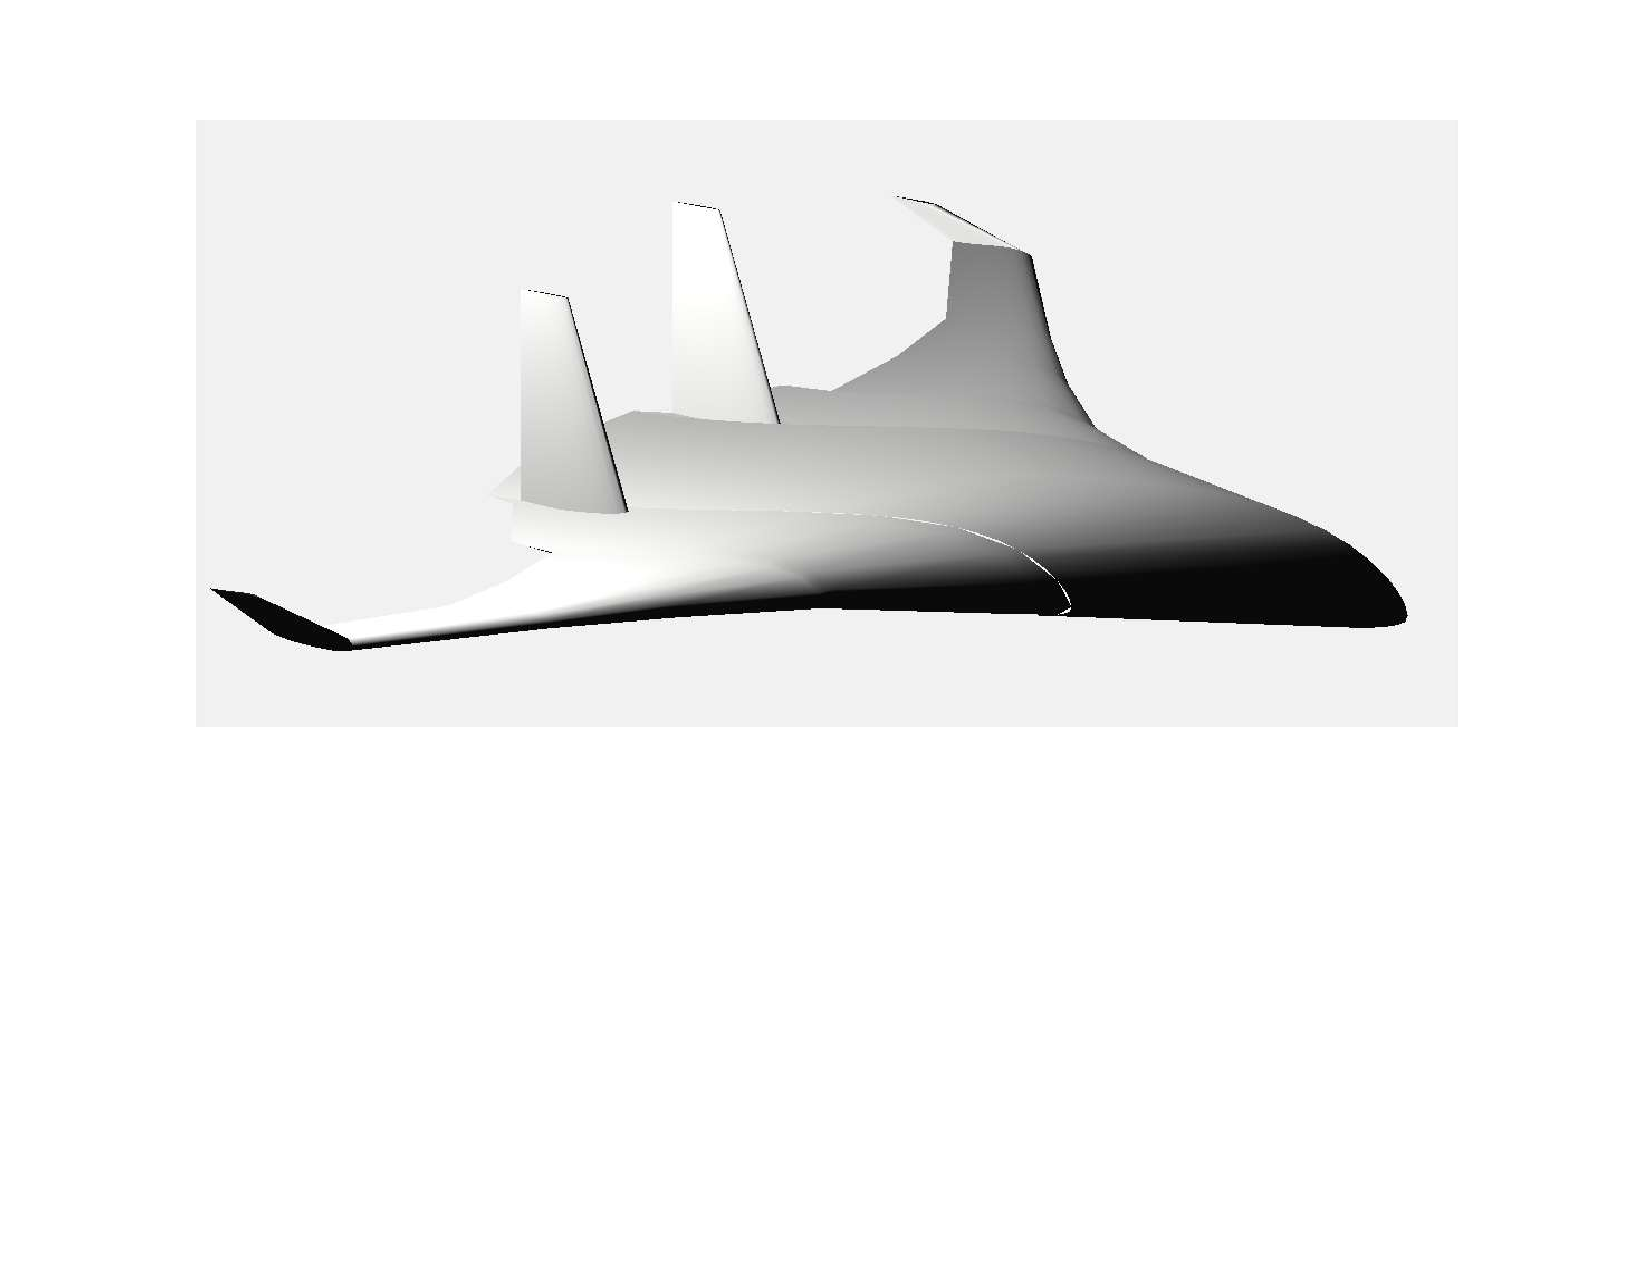
\includegraphics[scale=0.61]{Capitulo3/figs/ehekatl bwb g33 iso_cropped.pdf}
    \caption{EHEKATL BWB - Isometric view}
    \label{EHEKATL BWB G-33 Vista Isometrica}
\end{figure}

%\begin{figure}[!h]
%    \centering
%    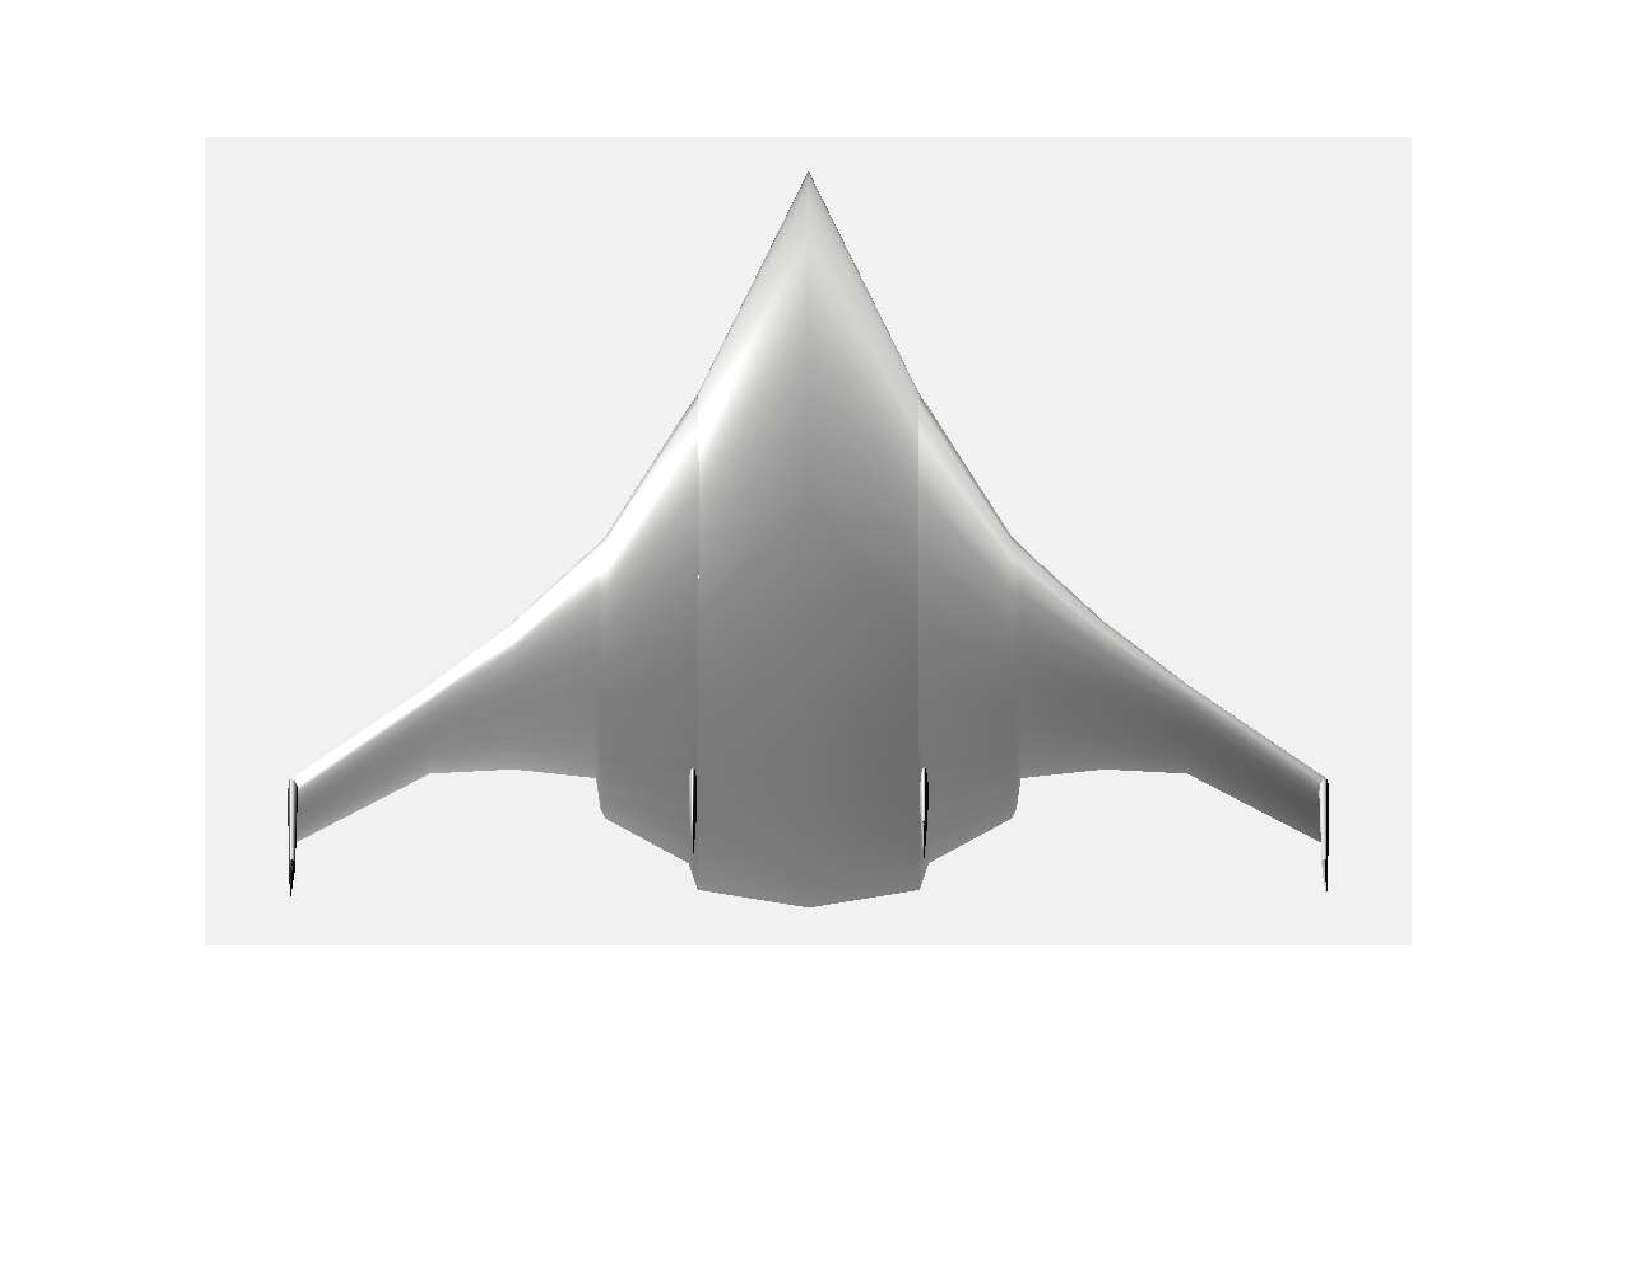
\includegraphics[scale=0.62]{Capitulo3/figs/ehekatl bwb g33 planta 1_cropped.pdf}
%    \caption{EHEKATL BWB - Vista de Planta}
%    \label{EHEKATL BWB G-33 Vista de Planta}
%\end{figure}

\begin{itemize}
    \item \textbf{Sweep or arrow angle.} Refers to the backward inclination of the wing with respect to a reference line (central line to or parallel to the fuselage), see Figure \ref{EHEKATL BWB G-33 Variables de Diseño} (b) A larger sweep (above 25);$^\circ$) can improve efficiency at high speeds and reduce air resistance. A moderate sweep (equal to or below 25$^\circ$) tends to be common in TAW aircraft, and can improve performance at cruise speeds while maintaining a robust structure. An excessive sweep angle can affect air flow distribution and stability. YB-49 and B-2 Spirit wing aircraft have an arrow of 45$^\circ$ and 55$^\circ$ respectively. \textbf{The proposed arrow angles for EHEKATL BWB are 63$^\circ$ in the central section and 54$^\circ$ in the outer wing}. 
    \item \textbf{Diedro angle.} It is the angle that forms each semi-wing with respect to the horizontal plane, see Figure \ref{EHEKATL BWB G-33 Variables de Diseño} (a) A positive diedro angle (wings tilted upwards) can increase lateral stability, as it tends to produce a restorative effect if the aircraft tilts laterally. In fly-wings and integrated wings, a modest diedro angle (equal to or less than 5$^\circ$) can contribute to greater lateral stability and better rotational behaviour. It is important to emphasize that the greater the stability less manoeuvrability, so finding a balance with respect to the flight mission is essential to guarantee the safety and integrity of the aircraft without substantially reducing its ability to degrees of freedom. \textbf{A dihedron of 3 is proposed$^\circ$ for EHEKATL BWB}. 
    \begin{figure}[!h]
    \centering
    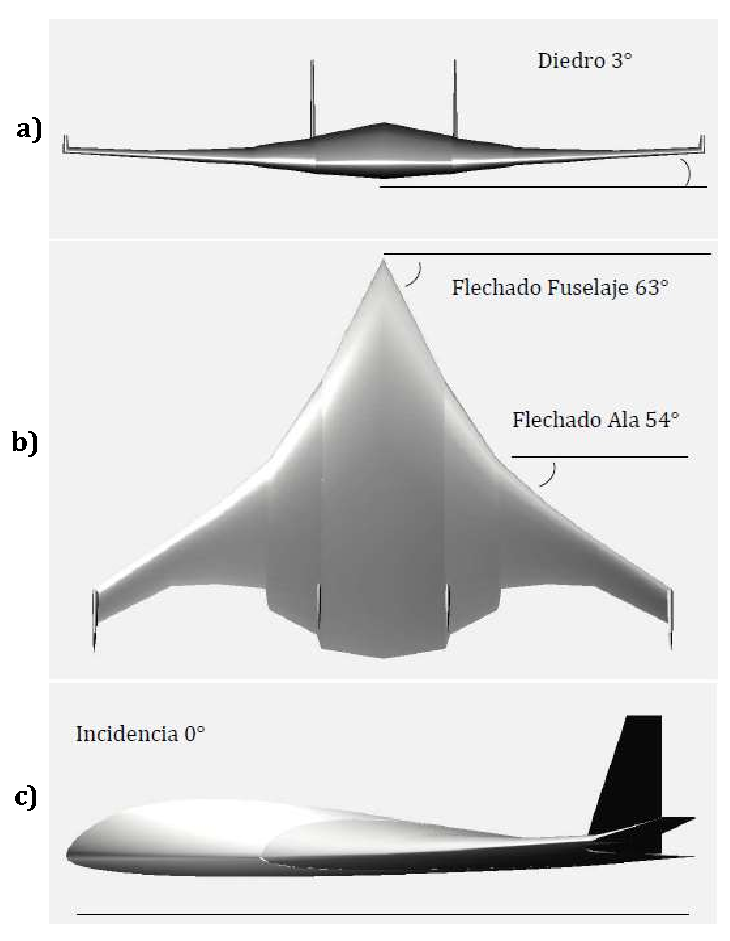
\includegraphics[scale=1.122]{Capitulo3/figs/ehekatl bwb g33 metricas 2.pdf}
    \caption{EHEKATL BWB - Design Variables}
    \label{EHEKATL BWB G-33 Variables de Diseño}
\end{figure}
    \item \textbf{Angle of Incidence.} It is the angle that forms between the wing rope and the direction of the relative airflow. This term is usually used as a synonym for the attack angle, as a design variable, we refer to the angle between the wing string and the central fuselage string (aerodynamic twist), see Figure \ref{EHEKATL BWB G-33 Variables de Diseño} (c) It directly affects the lift generated by the wing and, therefore, the performance of the flight. An appropriate angle of incidence is essential to ensure adequate support and stability in pitching. In wings-flyers and wings-integrated, this angle also influences how the aerodynamic loads are distributed along the aircraft. \textbf{The design proposal EHEKATL BWB in this thesis work seeks a minimalist proposal that meets the requirements of the aerodynamic design and opts for an incidence angle of zero}. 
    \item \textbf{Vertical stabilizers and fins at the tip of the wing.} Vertical stabilizers, also known as drifts, and fins at the wing tip are components that influence directional stability and balance control. In fly-wings and integrated wings, these components can help maintain stability on the vertical axis and control lateral drift. Their design, dimensioning and location are important to ensure stable and manoeuvrable behavior, as well as efficient aerodynamic performance. Although a larger reference area in vertical stabilizers and fins provides greater directional stability also increases drag, so it is essential to measure and locate properly. \textbf{EHEKATL BWB has vertical stabilizers with an area of 0.11 square meters. The fins were designed in order to minimize the vortex effect on the tip of the wing, as well as to take care of the pressure difference between the insides and the extrados.}. 
\end{itemize}

%\begin{figure}[!h]
%    \centering
%    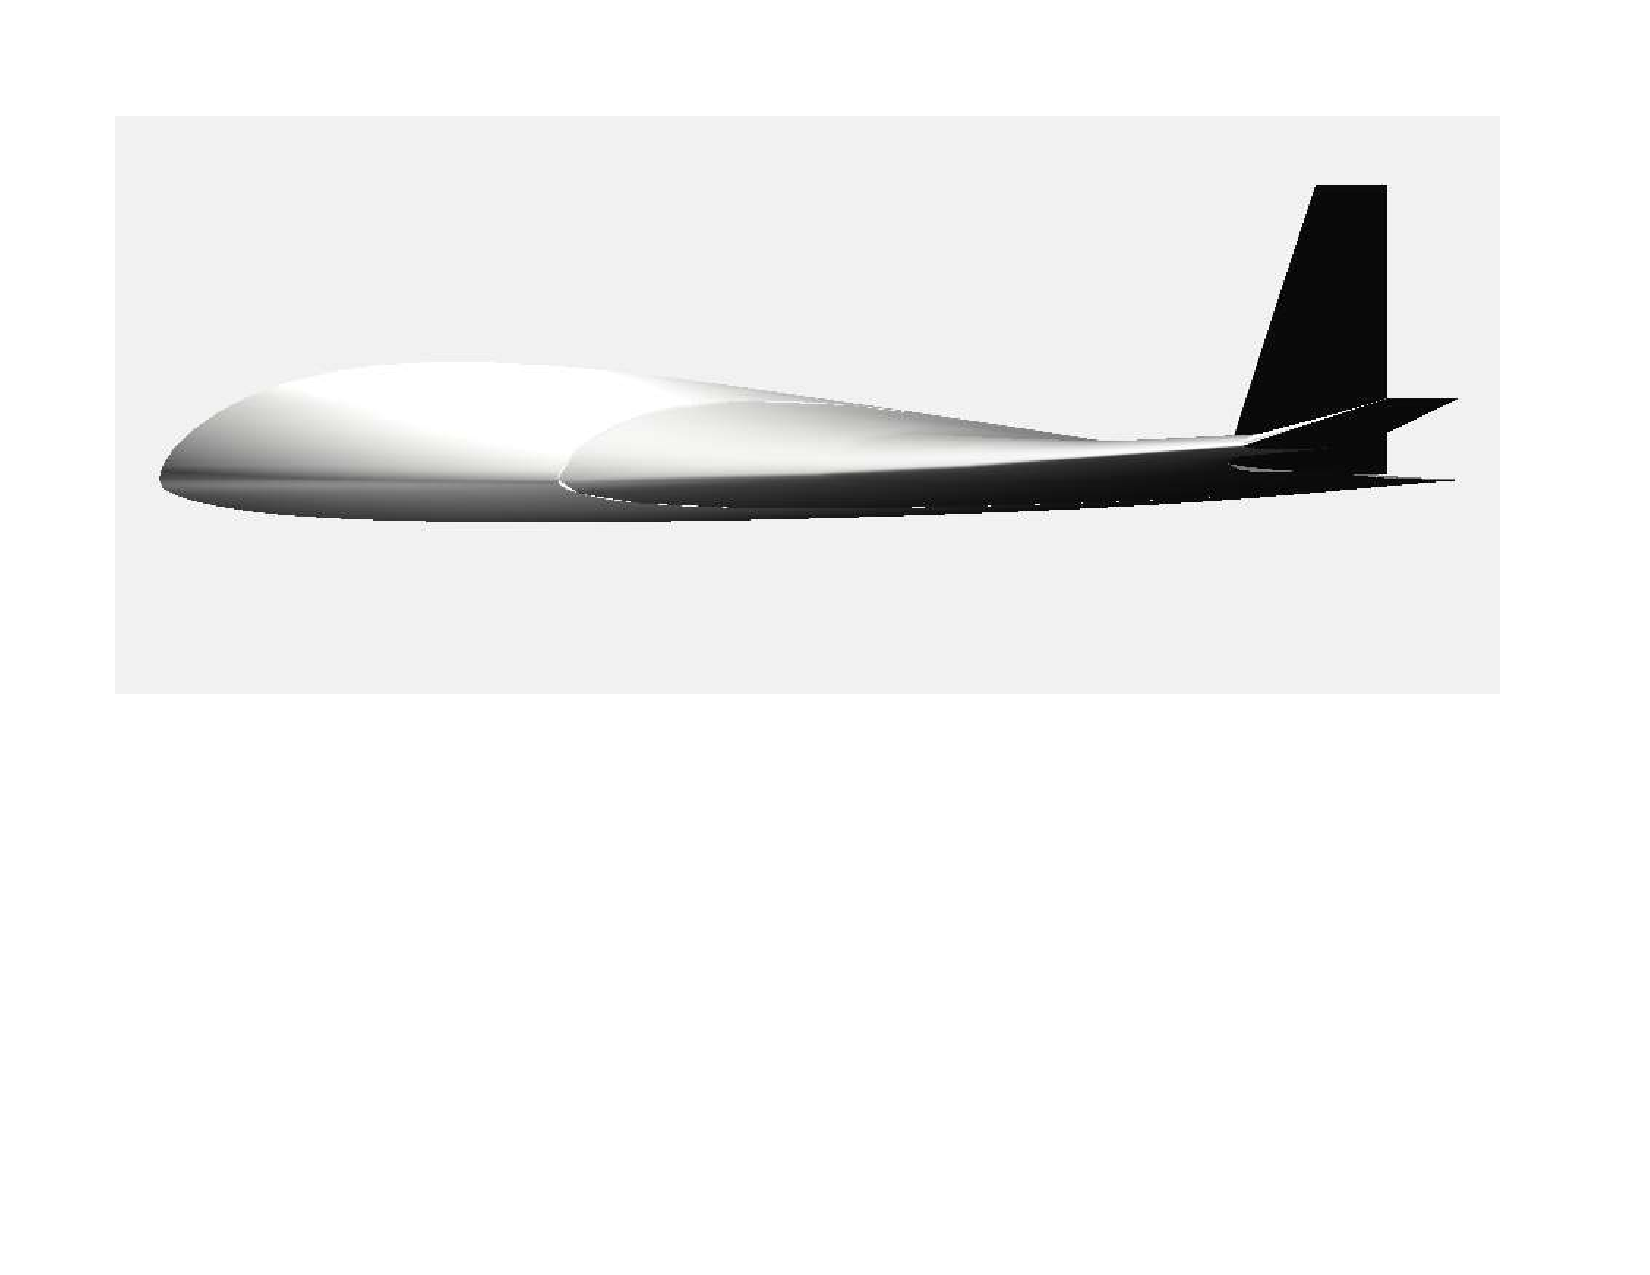
\includegraphics[scale=0.58]{Capitulo3/figs/ehekatl bwb g33 lateral_cropped.pdf}
%    \caption{EHEKATL BWB - Vista Lateral}
%    \label{EHEKATL BWB G-33 Vista Lateral}
%\end{figure}

The trailing edge of EHEKATL BWB is a particular geometry. If we start in plant view from the central fuselage rope to the wing tip of any semi-wing, we can appreciate four particular sections of such exit edge.
\textbf{The first section} It is the central one, where the two engines are planned to be located above, between the vertical stabilizers. Proposals where the stabilizers are integrated into the external structure of the engines are also common since they offer better aerodynamic performance due to a smaller frontal area between the integration of these two geometries (vertical motors and stabilizers).

\textbf{The second section} it is for the first control inputs (first elevons) that in this location are intended for its main function to be the moment of pitching (lifters).

\textbf{The third section} is the straight geometry on the trailing edge of the outer wing. Here are located two ACS which are intended for the most interesting flight phases, as they can offer multi-purpose functions (landing flaps and elevons for flight maneuvers). 

\textbf{The fourth section} is the last with only ACS intended mainly at the time of roll (alleron). 

General data on the aerodynamic design of EHEKATL BWB are shown in the Table \ref{EHEKATL BWB G-33 ficha geometrica}.

\begin{table}[!h]
    \caption{EHEKATL BWB - Geometric Design Data}
    \centering
    \begin{tabular}{|c|c|c|c|}
    \hline
    \multicolumn{4}{|c|}{EHEKAL BWB - Geometric Design}\\
    \hline
    Reference Area &  $1.4 m^2$ & Envergadura & $2.4m$  \\
    Long (fuselage or root rope) & $1.65m$ & Appearance Ratio & $3.9$ \\
    Conicity Relationship & $0.055$ & Angle Diedro & $3^\circ$ \\
    Angle Arrow Fuselage & $63^\circ$ & Angle Incidence & $0^\circ$ \\
    Angle Arrowed Wing & $54^\circ$ & Malla (Paneles) & $644$ \\
    Elevons & $8$ & Timones Direccionales & $2$ \\
    \hline
    \end{tabular}
    \label{EHEKATL BWB G-33 ficha geometrica}
\end{table}

%%%%%%%%%%%%%%%%%%%%%%%%%%%%%%%%%
\textbf{Mass distribution}\\ 
In the Table \ref{Distribucion de masas} the masses of each element of the avionics and energy system, and the quantity of each element, are shown. 
\begin{table}[!h]
    \centering
    \caption{Mass distribution}
    \begin{tabular}{|c|c|c|c|}
    \hline
    \textbf{Elemento} & \textbf{Masa (kg)} & \textbf{Cantidad} & \textbf{Masa Total (kg)} \\
    \hline
    Motores & 0.225 & 2 & 0.450 \\ 
    Bateria & 0.259 & 2  & 0.518 \\
    Autopiloto & 0.38 & 1 & 0.38 \\
    Graphic card & 0.25 & 1 & 0.25 \\
    Electronic Speed Controller & 0.125 & 2 & 0.250 \\
    Tubo Pitot & 0.05 & 1 & 0.05 \\
    Camera AI & 0.03 & 1 & 0.03 \\
    Servo-mecanismos & 0.021 & 10 & 0.21 \\
    \hline
    \multicolumn{3}{|c|}{ Mass in Empty} & 4.3\\
    \hline
    \multicolumn{3}{|c|}{Total Masses in Gravity Center} & 6.438\\
    \hline
    \end{tabular}
    \label{Distribucion de masas}
\end{table}
With "vacuum mass" reference is made to "vacuum weight", distinguishing the handling of mass and not force in this first approach. To understand why a vacuum mass of 4.3kg is defined it is recommended to go to the section of \ref{superficie alar y potencia requerida} \textit{Alar surface and required power}. It is important to remember that the design of aerial vehicles is an iterative process, so the relationship and interdependence between the different disciplines and calculations requires updating and validation for each iteration. The distribution of masses according to the geometry of EHEKATL BWB aims to locate the center of gravity in a strategic place for aerodynamic performance and stability. In EHEKATL BWB the distribution of masses is concentrated in two zones. In the front zone of the central body are located the auto-pilot, batteries, payload, electronic speed controllers, pitot tube and camera. In the back area are located the engines and servo-mechanisms that generate the movement of the ACS. This distribution locates the center of gravity of EHEKATL BWB G-33 to 0.83m from the \textit{Datum} or edge of attack. 


Table \ref{Coordendas de distribución de masas} shows the coordinates of the mass distribution in EHEKATL BWB. 
\begin{table}[!h]
    \centering
    \caption{ EHEKATL BWB - Mass Distribution Coordinates}
    \begin{tabular}{|c|c|c|c||c|c|c|c|}
    \hline
    \textbf{Description} & \textbf{x(m)} & \textbf{y(m)} & \textbf{z(m)} & \textbf{Description} & \textbf{x(m)} & \textbf{y(m)} & \textbf{z(m)} \\
    \hline
    Motor 1 & 1.6 & 0.072 & 0.01 & Motor 2 & 1.6 & -0.072 & 0.01 \\
    Bateria 1 & 0.5 & 0.2 & 0 & Bateria 2 & 0.5 & -0.2 & 0 \\
    ESC 1 & 0.5 & 0.069 & 0 & ESC 2 & 0.5 & -0.069 & 0 \\
    Autopiloto & 0.27 & 0 & 0 & Pitot & 0 & 0 & 0 \\
    Graphic card & 0.42 & 0 & 0 & Camera AI &  0.12 & 0 & -0.03  \\
    Serv-elevador 1 & 1.33  & 0.3 & 0 & Serv-elevador 2 & 1.33 & -0.3 & 0\\
    Serv-lift 1 & 1.3 & 0.55 & 0 & Serv-lift 2 & 1.3 & -0.55 & 0\\
    Serv-lift 3 & 1.3 & 0.72 & 0 & Serv-lift 4 & 1.3 & -0.72 & 0\\
    Serv-alleron 1 & 1.3 & 0.95 & 0 & Serv-alleron 2 & 1.3 & -0.95 & 0\\
    Serv-timon 1 & 1.5 & 0.12 & 0.12 & Serv-timon 2 & 1.5 & -0.12 & 0.12\\
    \hline
    \end{tabular}
    \label{Coordendas de distribución de masas}
\end{table}

To calculate the center of gravity are considered $n$ mass points $m_i$ with coordinates ($x_i, y_i, z_i$).  

\begin{equation}
   x_{c} = \frac{\sum_{i=1}^{n} m_i \cdot x_i}{\sum_{i=1}^{n} m_i} 
\end{equation}

\begin{equation}
    y_{c} = \frac{\sum_{i=1}^{n} m_i \cdot y_i}{\sum_{i=1}^{n} m_i}
\end{equation}

\begin{equation}
   z_{c} = \frac{\sum_{i=1}^{n} m_i \cdot z_i}{\sum_{i=1}^{n} m_i} 
\end{equation}

\begin{figure}[!h]
    \centering
    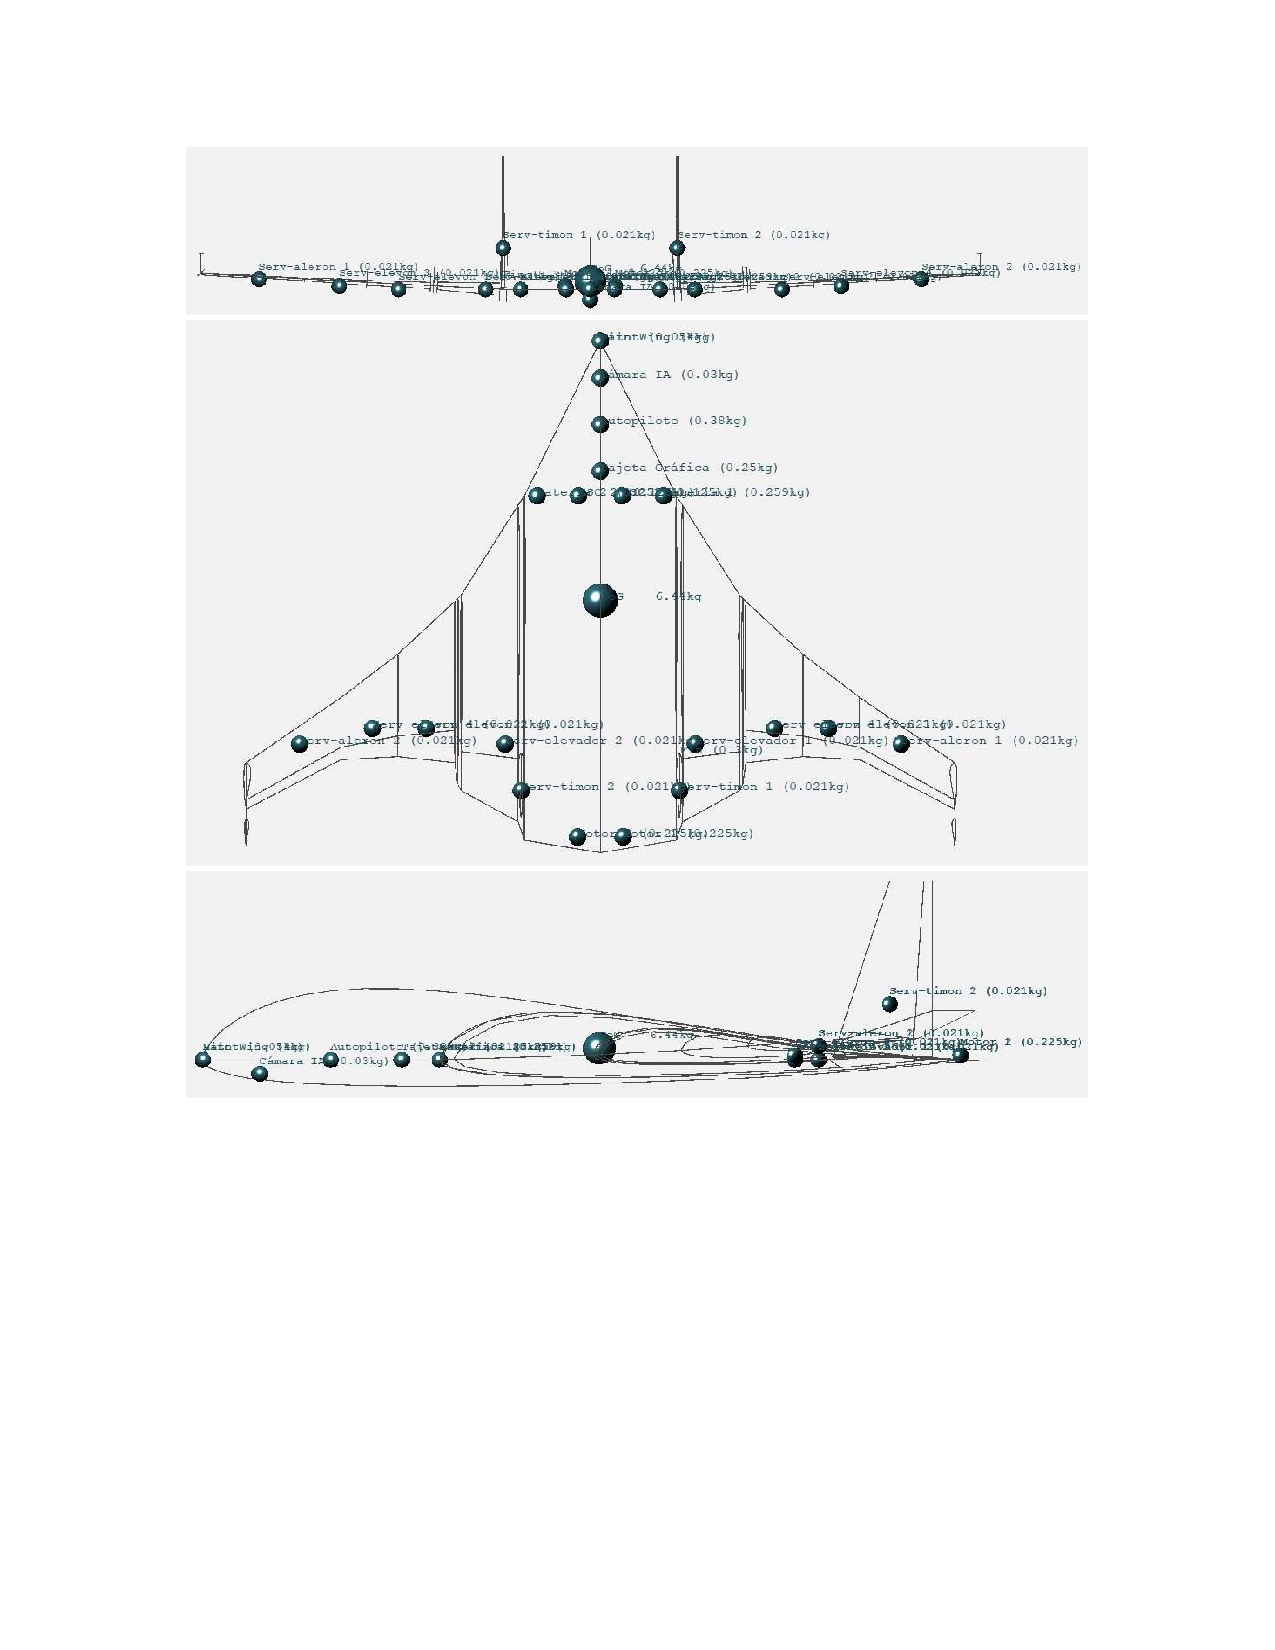
\includegraphics[scale=0.9]{Capitulo3/figs/distribucion de masas_cropped.pdf}
    \caption{Mass distribution}
    \label{Distribución de masas}
\end{figure}

According to the data in the Tables \ref{Distribucion de masas} and \ref{Coordendas de distribución de masas} the following results are obtained in the calculation of the centre of gravity. 
\begin{align}
    x_c &= 0.7473 m \\ \nonumber
    y_c &= 0.0 m \\ \nonumber
    z_c &= 0.0002 m \nonumber
\end{align}
\textbf{The centre of gravity calculated by XFLR5 shows the following coordinates:} $x_C=0.8315$, $y_c=0.0m$ and $z_c = 0.0025$. The differences between the analytical calculation and the calculation with XFLR5 are due to the fact that in the analytical calculation only the avionic masses and the energy system are considered, while XFLR5 in addition to these also contemplates the location and mass of the vertical stabilizers (0.15kg each). The vacuum mass of EHEKATL BWB integrates the mass of the entire aircraft volume (body and stabilizers) defined in section \ref{superficie alar y potencia requerida}. If the mass and coordinates of the vertical stabilizers are considered in the analytical calculation, the approximation obtained with XLR5 is obtained. \ref{Distribución de masas}the distribution of the elements of the avionics and energy system according to their mass, and the center of gravity as a result, is shown.


\medskip

\textbf{Simulations and Aerodynamic Parameters}\\
The efficient and effective design of aircraft is a highly complex and multidisciplinary process that requires a deep understanding of the dynamic aerodynamic and fluid phenomena that influence their performance. For the aerodynamic simulations of EHEKATL BWB the speeds of the Table are set \ref{tab: Re y velocidades} under the environmental conditions of the Table \ref{tab: Propiedades del aire en UPMH a $z=2,426m$ } and that are represented with the type of line in the Figure \ref{Tipo de línea de acuerdo con la técnica de simulación y la velocidad}. 

Before analyzing the aerodynamic results of EHEKATL BWB it is important to remember that there are three key points according to mass distribution, geometry and aerodynamic forces: centre of gravity (CG), neutral point (NP) and center of pressure (CP). 
%
The \textbf{pressure centre} is the point resulting from applied aerodynamic forces. It depends on the aerodynamic model and angle of attack.
%
The \textbf{centre of gravity} is the point where the moments act, depends only on the mass distribution of the aircraft and not on its aerodynamics.
%
The \textbf{punto neutro} It is the point of reference where the timing does not depend on the angle of attack. It depends only on the external geometry of the aircraft. Now we will define the stability of the aircraft according to the direction of the wind and the position ratio of the center of gravity and neutral point.
%
Si \textbf{CG ahead of NP} The pressure force on the aircraft matches the direction of the aircraft, but in the opposite direction. Very stable.
%
Si \textbf{CG slightly ahead of NP} the pressure force on the aircraft matches the direction of the aircraft, but in the opposite direction. Stable but wind-sensitive.
%
Si \textbf{CG matches NP:} The aircraft could rotate indefinitely.
%
Si \textbf{CG behind the NP} We have stability but in the opposite direction, \cite{Deperrois2010}.
%
Figure \ref{EHEKATL BWB - Centro de Gravedad, Centro de Presiones y Punto Neutro} represents the change of position of the pressure centre according to the change in the angle of attack at constant speed. The centre of gravity remains constant according to the mass distribution, and the neutral point remains constant according to the geometry of EHEKATL BWB. 
\begin{figure}[t]
    \centering
    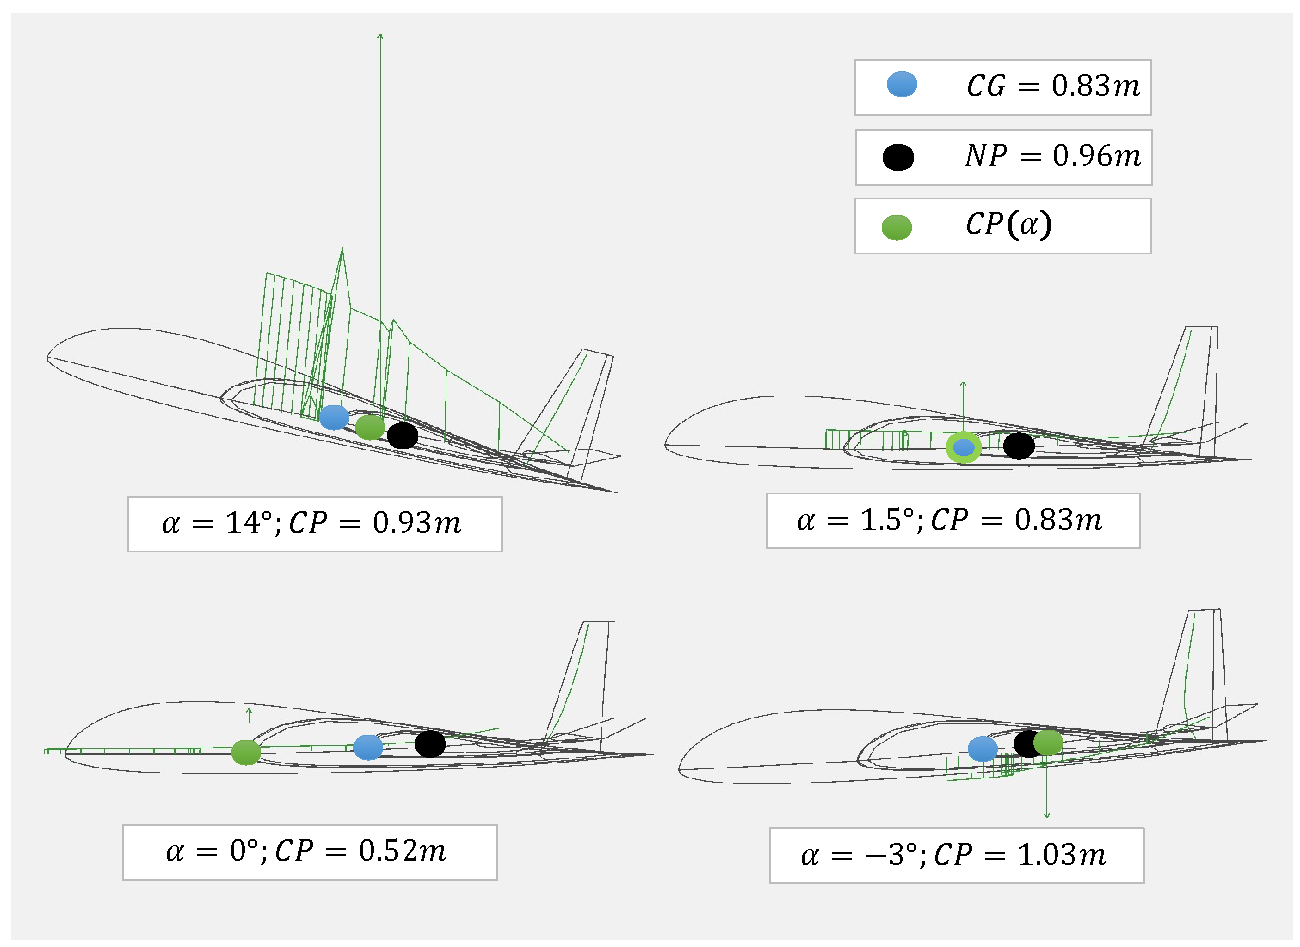
\includegraphics[scale=0.65]{Capitulo3/figs/CG CP NP.pdf}
    \caption{EHEKATL BWB - Gravity Center, Pressure Center and Neutral Point}
    \label{EHEKATL BWB - Centro de Gravedad, Centro de Presiones y Punto Neutro}
\end{figure}

The average aerodynamic rope\footnote{Mean Aerodynamic Chord or MAC} refers to the average length of the cross-section of the wing of an aircraft. Since EHEKATL BWB has pronounced arrow angles, the calculation of the MAC is essential.
%
Figure \ref{Desplazamiento del Centro de Presiones de acuerdo la variación del ángulo de ataque} shows the variation of the pressure centre in relation to the angle of attack. The calculation of the MAC with XFLR5 is 0.96m. It can be seen that the pressure center tends to this value according to the angle of attack increases, and also when it decreases. When the angle of attack is between 0 and -1 an asynthotic behavior with erratic oscillations is observed. In conclusion, the location of the pressure center approaches the MAC as the angle of attack increases or decreases, but in the aforementioned interval the point of application for the generation of support is not defined. 

\begin{figure}[!h]
    \centering
    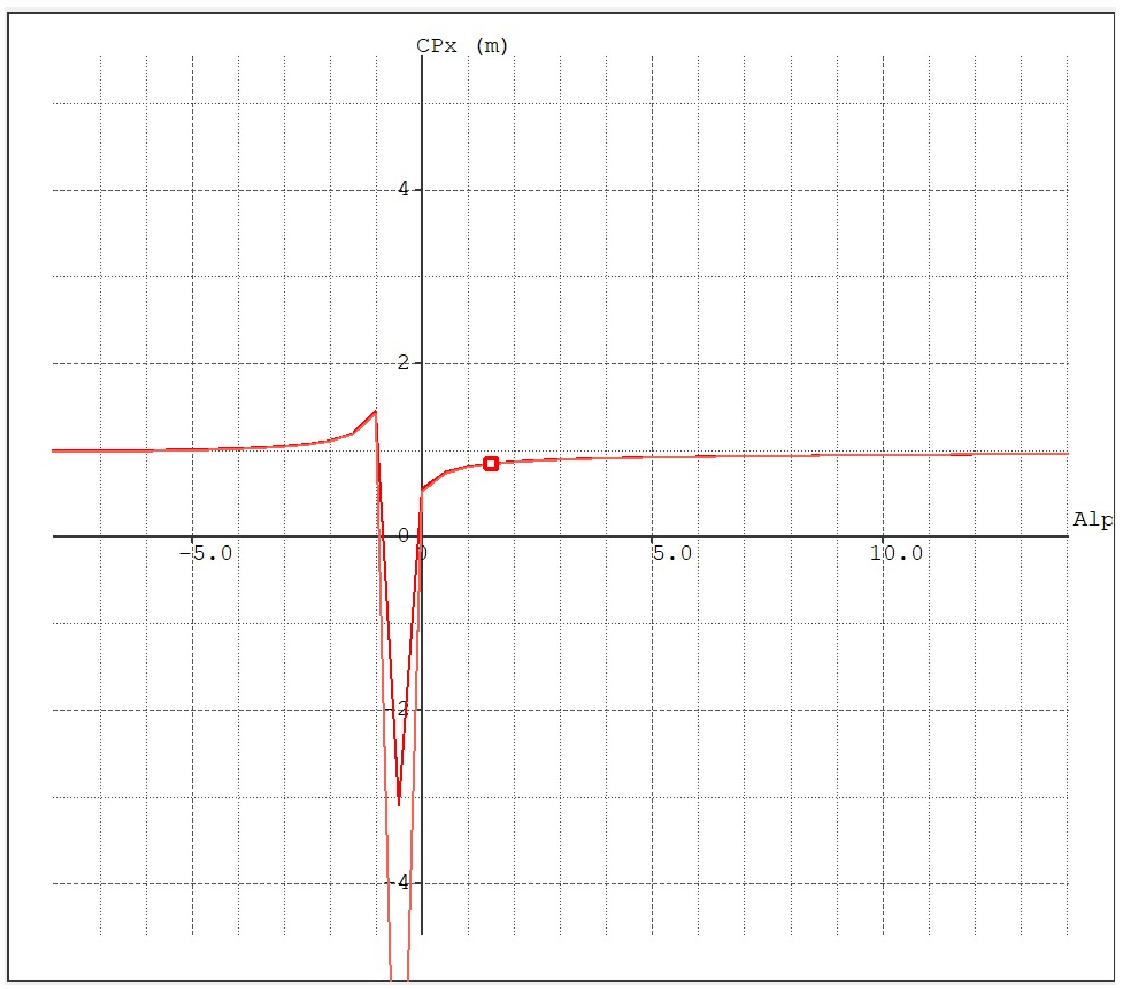
\includegraphics[scale=0.65]{Capitulo3/figs/cp alpha.pdf}
    \caption{Movement of the Pressure Center according to the variation of the angle of attack}
    \label{Desplazamiento del Centro de Presiones de acuerdo la variación del ángulo de ataque}
\end{figure}

\medskip

The \textbf{similarity parameters} in the context of aircraft design they refer to the dimensional and flow ratios that must be maintained constant between a scale model and the aircraft at real size so that the test results in wind tunnels in the scale model are representative of the behaviour of the actual aeroplane. In this context, the two most important similarity parameters are the Reynolds Number (Re) and Mach Number. Although, the scale provided in the Table \ref{EHEKATL BWB G-33 ficha geometrica} is considered the actual scale for flight missions in the UPMH, it is important to define the number of Re and Mach to know the dimensional and flow ratio of EHEKATL BWB.
%
Calculations of Dimensional Parameters $Re$ and $Mach$ were calculated on the basis of the following functions: 
\begin{equation}
    Re =  \frac{\rho c V}{\mu}
\end{equation}
\begin{equation}
    Mach = V / a
\end{equation}
where $V$ is the speed of the aircraft, $\rho$ is the density of the fluid, $c$ It's the profile rope, $\mu$ is the viscosity of fluid and $a$ It is important to mention that viscosity varies according to the temperature of the fluid but is practically independent of its pressure.

The formula for calculating the speed of sound is as follows:
\begin{equation}
    a = 331.3 \sqrt{1 + \frac{T}{273.15}}
\end{equation}
Considering the temperature $T$ in degrees Celsius. 

The defined speed range for EHEKATL BWB is shown in the Table \ref{tab: Re y velocidades} regarding the minimum and maximum number of Re, considering the rope at the tip of the fin and the root rope respectively. Also, the number of Mach is shown according to the defined speeds and the environmental conditions of the Table \ref{Datos de entrada para simulación en XFLR5 de EHEKALT BWB G-33}, input data for the simulations of the EHEKATL BWB aircraft.   
\begin{table}[!t]
    \centering
     \caption{Speeds and similarity parameters for the aerodynamic simulations of EHEKATL BWB}
    \begin{tabular}{|c|c|c|c|}
    \hline
     \textbf{Velocidad} & \textbf{Reynolds - Root} & \textbf{Reynolds - Punta} & \textbf{Mach} \\
     \hline
     \textit{Loss} $19 m/s$ & $1,963,213$ & $107,084$  & $0.057$\\
     \textit{Despegue} $22 m/s$ & $2,273,194$ & $123,992$  & $0.066$\\
 \textit{Crucero} $27 m/s$ & $2,789,829$ & $152,163$  & $0.081$\\
     \textit{Maximum} $35 m/s$ & $3,616,445$ & $197,261$  & $0.105$\\
     \hline
    \end{tabular}
    \label{tab: Re y velocidades}
\end{table}
\begin{figure}[!h]
    \centering
    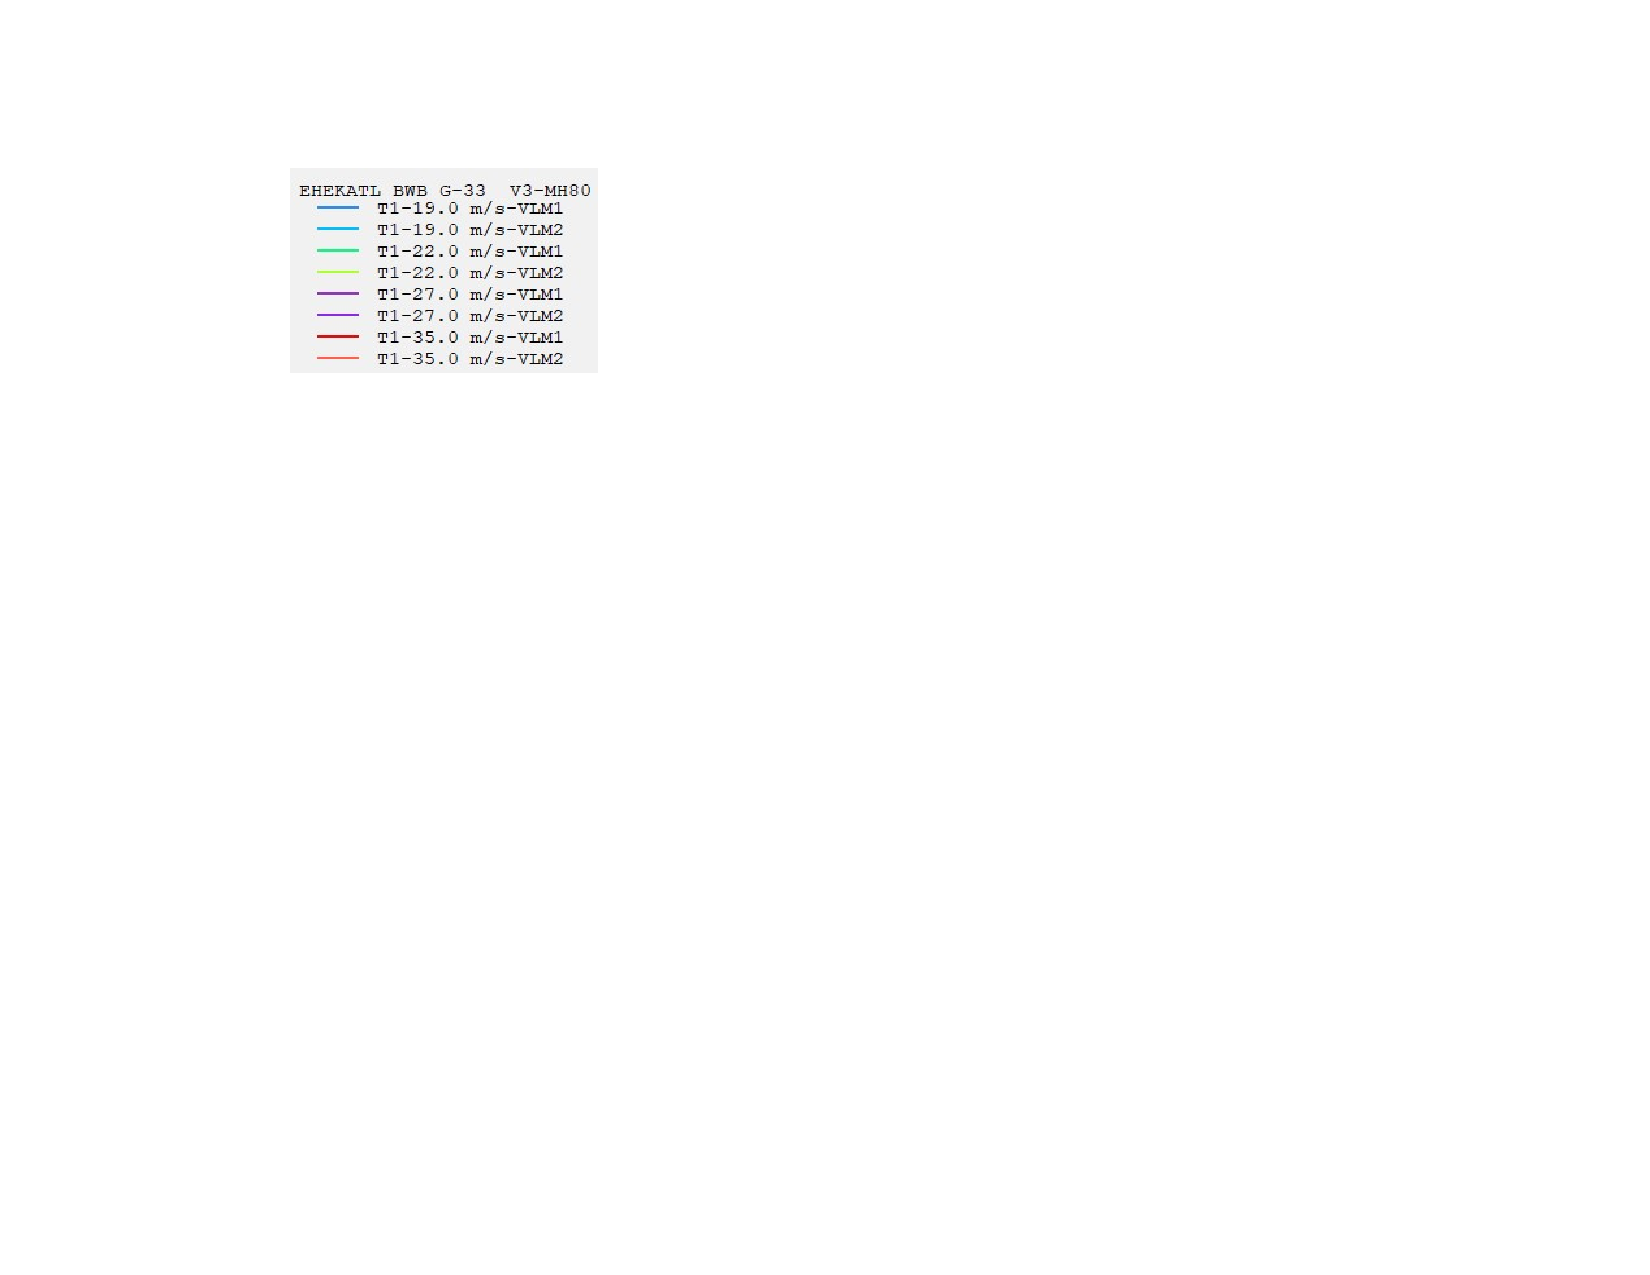
\includegraphics[scale=1.2]{Capitulo3/figs/lineas de simulaciones (1).pdf}
    \caption{Line type according to simulation technique and speed}
    \label{Tipo de línea de acuerdo con la técnica de simulación y la velocidad}
\end{figure}

\begin{table}[t]
    \centering
    \caption{Input data for XFLR5 simulation by EHEKALT BWB}
    \begin{tabular}{|c|c|c|}
    \hline
    \multicolumn{3}{|c|}{Fluid parameters (air) in XLR5} \\
    \hline
    Concepto & Cantidad & Unidad \\
    \hline
    Temperatura & -0.8 & $^{\circ}C$  \\
    Altitud & 2,426 & $m$ \\
    Pressure & 75,379.9 & $Pa$ \\
    Densidad & 1.02344 & $kg/m^3$ \\
    Dynamic viscosity & $1.63e05$ & $kg/ms$ \\
    Cinematic viscosity & $1.59e05$ & $m^2/s$ \\
    Sound Speed & 330.8 & $m/s$ \\
    \hline
    \end{tabular}
    \label{Datos de entrada para simulación en XFLR5 de EHEKALT BWB G-33}
\end{table}

The root cord is from $1.65m$, the rope at the tip of the wing is from $0.15m$ and at the tip of the fin $0.9m$.
%
In the Figure \ref{Tipo de línea de acuerdo con la técnica de simulación y la velocidad} Line types (colors) can be seen according to speed and simulation type. VLM1 and VLM2 simulations were used. In the appendices section \ref{Simulaciones con XFLR5} the properties of simulation techniques in XFLR5 and their limitations are explained. The speeds set for EHEKATL BWB were for the purpose of obtaining the highest possible performance and complying with the regulations of the \textit{FAA} for smaller scale VANTS (Non-Study Aerial Vehicles). 
\textbf{The speed limit set by the \textit{FAA} is from $160km/h$, and the maximum speed of EHEKATL BWB is $126km/h$, approximately the $10\%$ of the speed of sound}.



The \textbf{Reynolds number} represents the relationship between inertial and viscous forces in the flow around an object. $Re$ is an adimensional value through which we can determine the nature of the viscose boundary layer, i.e. whether the airflow is laminar or turbulent. When two objects have the same number of Reynolds, they experience similar flow patterns, be it laminar or turbulent. This is crucial in the aerodynamic design, both of the wing and control surfaces, where flow properties are essential for efficiency and performance.

The \textbf{Mach number} When two objects or configurations have the same Mach number, they are experiencing similar aerodynamic conditions in terms of shock waves, compressibility, and phenomena associated with sound speed. This is essential for the design and testing of aircraft and space vehicles, where flow speed and compressibility are crucial factors. The interest ranges of the Mach number are
\begin{itemize}
    \item Subsonic : $Mach < 1.0$
    \item Transonic : $0.8 < Mach < 1.2$
    \item Supersonic : $1.0 < Mach < 5.0$
    \item Hypersonic : $5.0 > Mach$
\end{itemize}

The \textbf{compresibilidad} and the \textbf{viscosidad} are two aerodynamic phenomena that have a significant impact on air vehicle behaviour.
%
Compressibility refers to the change in air density due to variations in speed, temperature or pressure. At higher speed, such as transonic or hypersonic, compressibility effects become more prominent and can lead to phenomena such as shock waves formation and loss of aerodynamic efficiency. \textbf{EHEKATL BWB are operating at very low speeds (0.05-0.1 Mach)}, in this range, compressibility effects are relatively insignificant, and can be ignored to simplify aerodynamic analysis. 

Viscosity is a property of fluids that refers to the internal resistance of fluid when flowing. In simpler terms, it is the "stickiness" of fluid. A highly viscous fluid has a significant resistance to movement, while a low viscosity fluid flows more easily. The viscosity of air is relatively low compared to other fluids such as water, but still has an impact on aerodynamics, especially in the boundary layer and in the formation of shock waves. 
\textbf{In the case of EHEKATL BWB and according to the Reynolds and Mach numbers in the Table \ref{tab: Re y velocidades}, viscosity is an important consideration in aerodynamic analysis}. Specifically, in the boundary layer, viscosity has a significant impact on the resistance and flow behavior around the aircraft. However, viscosity effects are not as dominant as at lower speeds or in transonic or supersonic conditions. 


The first result shown in the Figure \ref{Coeficiente de lift (levantamiento) respecto al ángulo de ataque de EHEKATL BWB}, is the coefficient of support or lifting $C_L$ from EHEKATL BWB. 
\begin{figure}[!t]
    \centering
    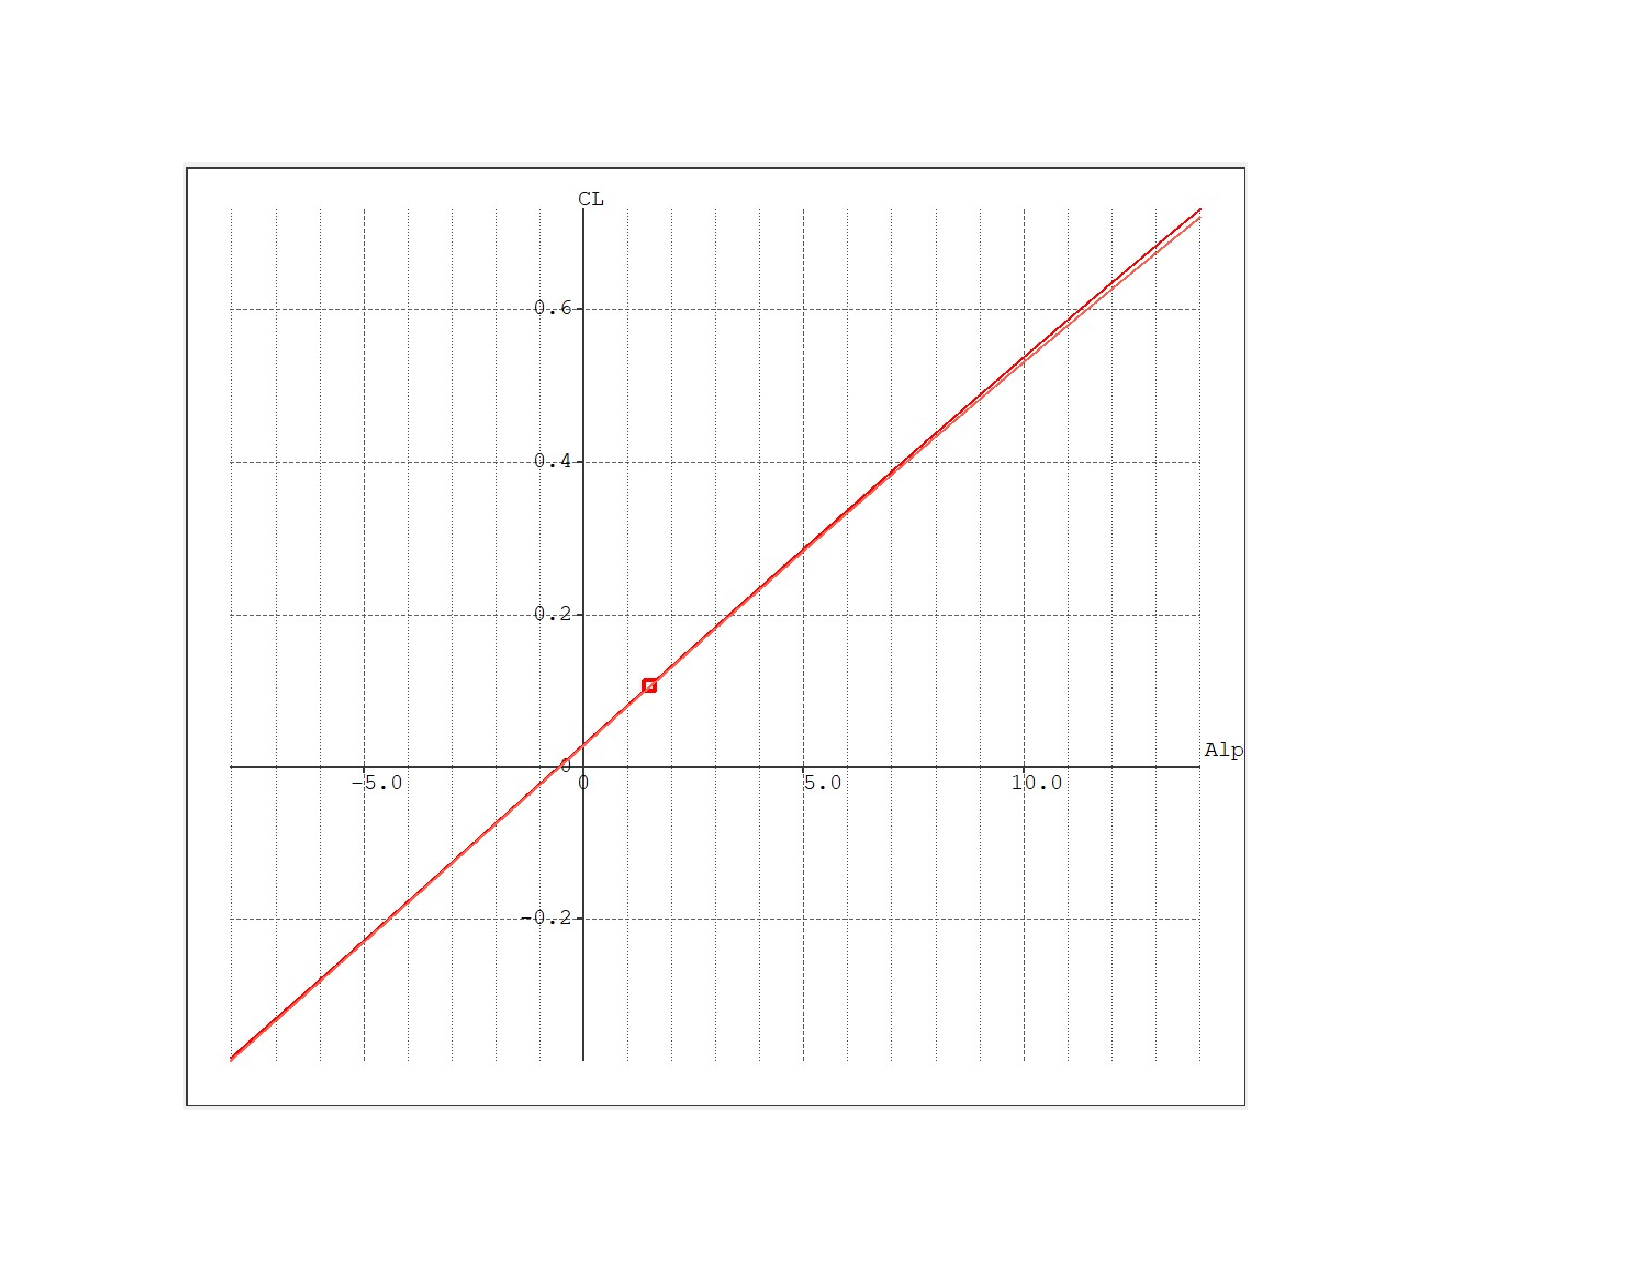
\includegraphics[scale=0.75]{Capitulo3/figs/CL ehekatl (1).pdf}
    \caption{EHEKATL BWB - Lift coefficient}
    \label{Coeficiente de lift (levantamiento) respecto al ángulo de ataque de EHEKATL BWB}
\end{figure}
The lifting coefficient is an adimensional parameter that describes the ability of a profile or aircraft to generate support. The lifting coefficient is defined as the relationship between the lift (L), the reference area (S) of the supporting surface, density ($\rho$) and the speed of air flow (V) around the body,
\begin{equation}
    C_L = \frac{L}{\frac{1}{2} \rho V^2 S}
\end{equation}
in the Figure \ref{Coeficiente de lift (levantamiento) respecto al ángulo de ataque de EHEKATL BWB} We have the EHEKATL BWB lift coefficient for the 4 speeds proposed in the Table. \ref{tab: Re y velocidades} and its graphical relationship to line type in the Figure \ref{Tipo de línea de acuerdo con la técnica de simulación y la velocidad}. All speeds were simulated with both methods, VLM1 and VLM2. In Figure \ref{Coeficiente de lift (levantamiento) respecto al ángulo de ataque de EHEKATL BWB} Two main lines are perceived, the line that meets the values above is the results obtained corresponding to the VLM1 method. All the speeds gave a similar lifting coefficient, therefore, only two lines are perceived, the speeds resolved with the VLM1 and VLM2 method. 

If we consider the variation in the angle of attack, we have the coefficient of elevation depending on the angle of attack denoted. $C_L(\alpha)$. The relationship between the lifting coefficient and the angle of attack is often represented by a curve known as the polar holding curve
\begin{equation}
    C_L (\alpha) = a \alpha + C_{L0}
\end{equation}
where:
$a$ is the slope of the polar supporting curve, $\alpha$ is the angle of attack and $C_{L0}$ is the lifting coefficient when the angle of attack is zero. It is important to note that the function $C_L (\alpha)$ just consider the simplification of the linear model, which is the result we got with XLR5 and consider a range of $\alpha$ between -8$^\circ$ 14$^\circ$.  

In the Figure \ref{Coeficiente de arrastre de EHEKATL BWB} the simulation results of EHEKATL BWB according to the drag coefficient are available. 
\begin{figure}[!t]
    \centering
    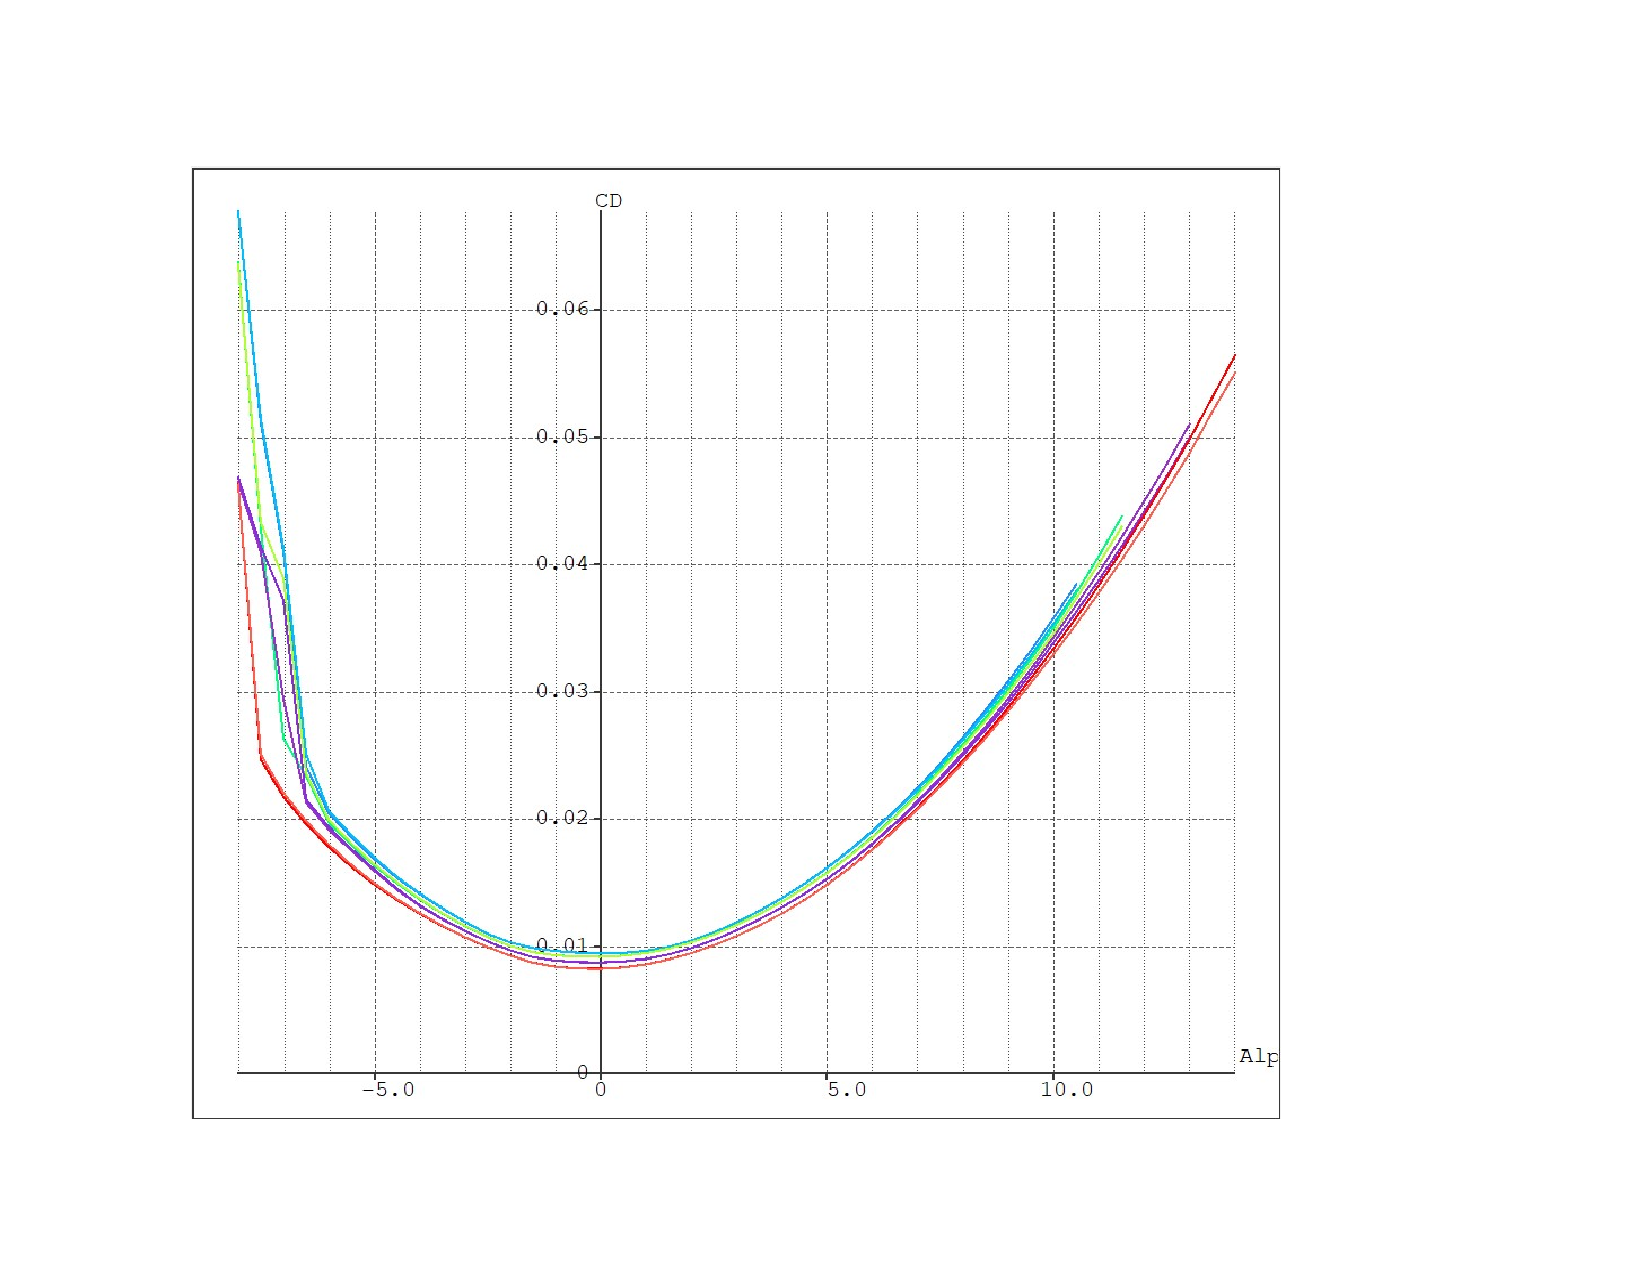
\includegraphics[scale=0.75]{Capitulo3/figs/arrastre ehekatl.pdf}
    \caption{EHEKATL BWB - Trawl coefficient}
    \label{Coeficiente de arrastre de EHEKATL BWB}
\end{figure}
The drag coefficient is the amount of resistance the aircraft body faces when moving through the fluid, air
\begin{equation}
    C_D = \frac{D}{\frac{1}{2} \rho V^2 S}
\end{equation}
where $D$ is the strength of resistance or drag. It consists of two main components: the viscous drag coefficient $C_{D_0}$ and the induced drag coefficient $C_{D_i}$. \footnote{In the section of \textit{Alar surface and required power} We exhaustively develop the calculation of the viscous and induced drag.}
\begin{equation}
    C_D = C_{D_0} + C_{D_i}
\end{equation}
\begin{figure}[!h]
    \centering
    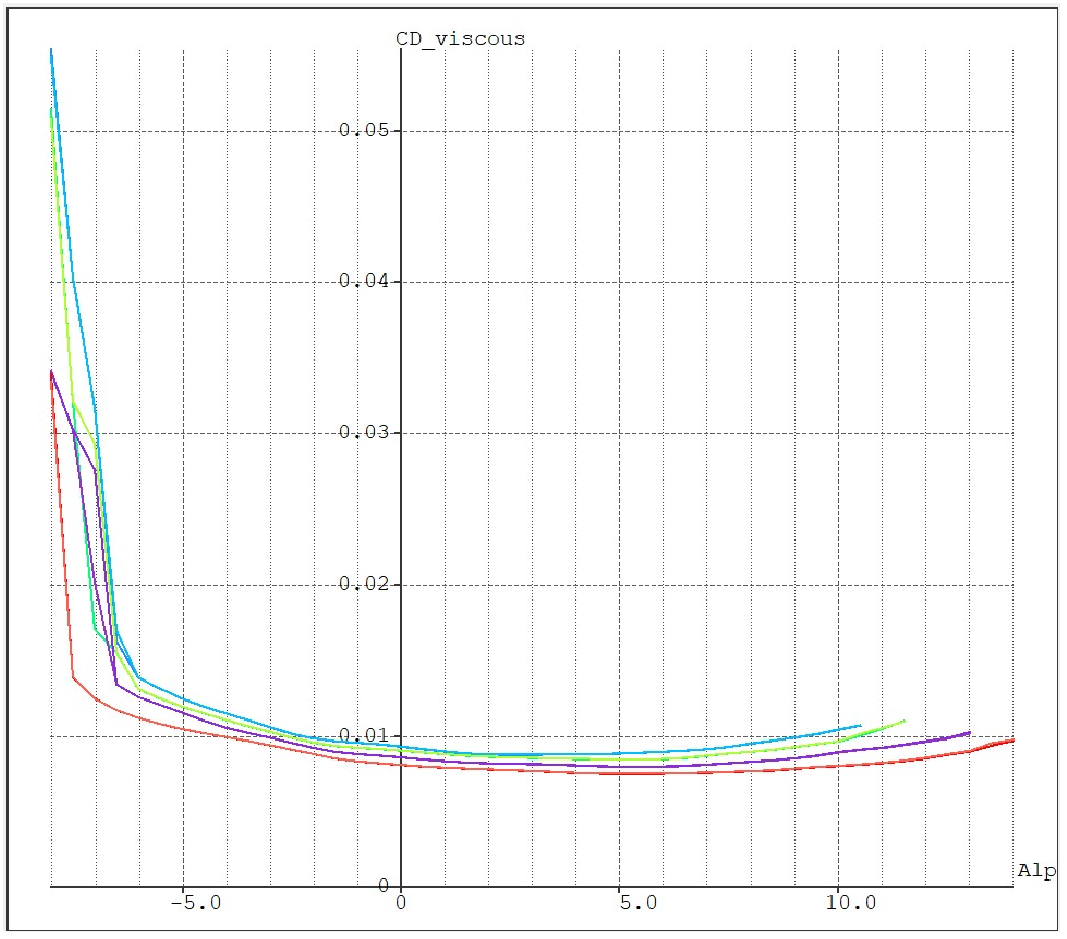
\includegraphics[scale=0.75]{Capitulo3/figs/arrastre viscoso ehekatl.pdf}
    \caption{EHEKALT BWB - Viscous trawl coefficient}
    \label{Coeficiente de arrastre viscoso}
\end{figure}
The viscous drag coefficient is associated with friction between the body and the surrounding fluid. It depends on the shape of the body and the viscosity of the fluid. For aerodynamic profiles, this component tends to decrease as the number of Reynolds increases. The induced drag coefficient is associated with the production of vortexes and the generation of support. It increases with the angle of attack and with the efficiency of the support distribution in the aircraft. The angle of attack influences both components of the drag coefficient. 
\begin{figure}[!h]
    \centering
    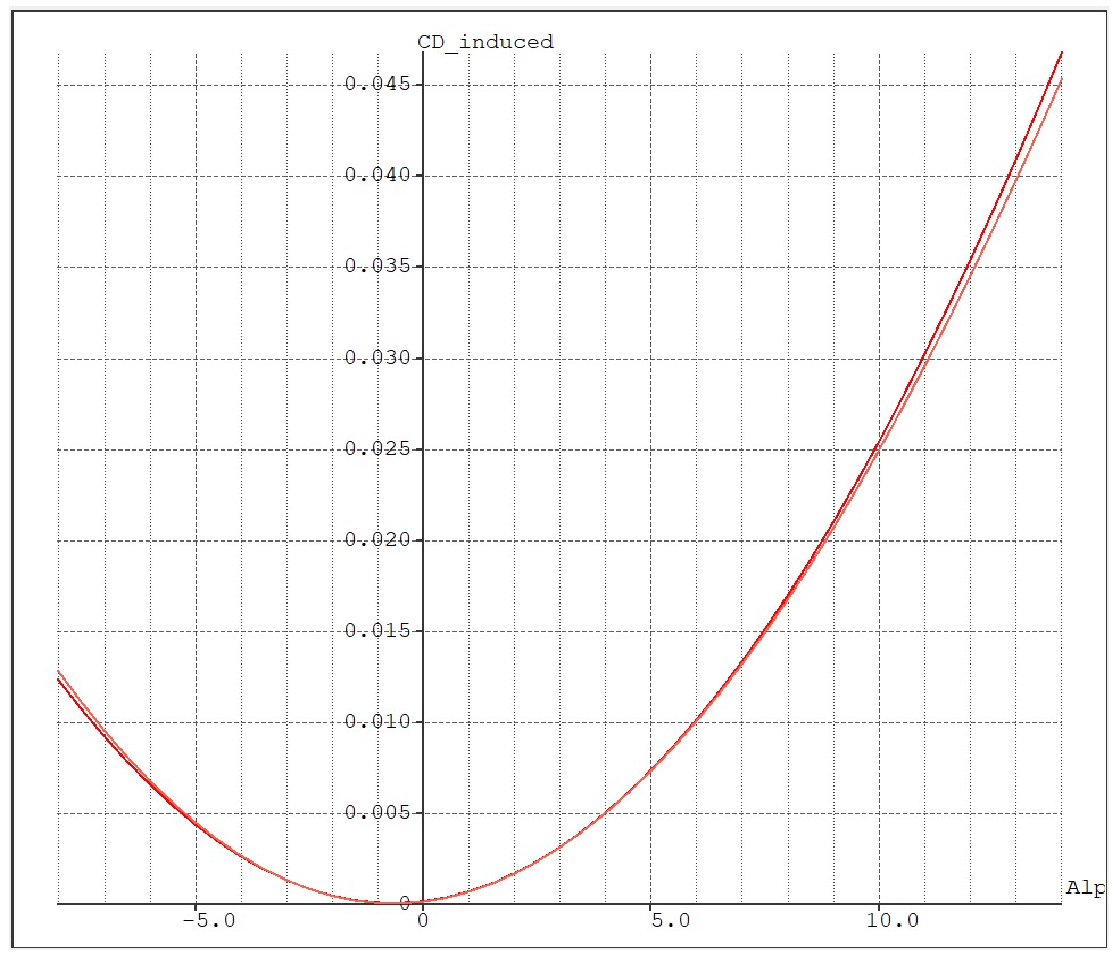
\includegraphics[scale=0.75]{Capitulo3/figs/arrastre inducido ehekatl.pdf}
    \caption{EHEKALT BWB - Induced drag coefficient}
    \label{Coeficiente de arrastre inducido}
\end{figure}
As the angle of attack increases, the total drag coefficient increases due to an increase in support and, therefore, in the induced drag. However, the viscous drag coefficient given the geometry of EHEKATL BWB throws a value that goes down slightly to then ascend, but that within the range of interest of the angle of attack we could consider as constant. 

The reason for $C_L$ (lift coefficient) compared to $C_D$ (drag coefficient) is a measure that provides information on the aerodynamic efficiency of an object or aircraft. This ratio is known as aerodynamic efficiency or sustainability efficiency and is an important indicator in the design of EHEKATL BWB and its performance. In simple terms, it represents how much support is generated by each drag unit produced. This reason is especially important in the design of aircraft, as it influences aspects such as the scope, fuel economy and cargo capacity of an aircraft.

The relationship $C_L / C_D$ depending on the angle of attack is a graphic representation showing how the aerodynamic efficiency of an aircraft varies as the angle of attack is changed. In a graph you see several regions of interest:

Region of Ascenso (Slope-Up Region): In this region,  $C_L$ increases as the angle of attack increases, which means that more support is being generated. $C_D$ also increases, indicating a greater drag. Aerodynamic efficiency $C_L/C_D$ It goes down.

Max Lift Point: This is the point on the graph where aerodynamic efficiency $C_L/C_D$ represents the angle of attack at which the aircraft generates maximum support per drag unit.

Region of Descenso (Slope-Down Region): After the maximum support point, if the angle of attack continues to increase, the aerodynamic efficiency decreases.  $C_L$ continues to grow, but 
$C_D$ increases at a faster rate, indicating a loss of efficiency.

The importance of the relationship $C_L/C_D/\alpha$: The maximum holding point is critical for the take-off and landing of an aircraft, as it indicates the optimum angle of attack to generate the greatest support with the least possible drag. The shape of the curve $C_L/C_D/\alpha$ It may also provide information on the manoeuvrability and behaviour of an aircraft at different flight stages.

\begin{figure}[!t]
    \centering
    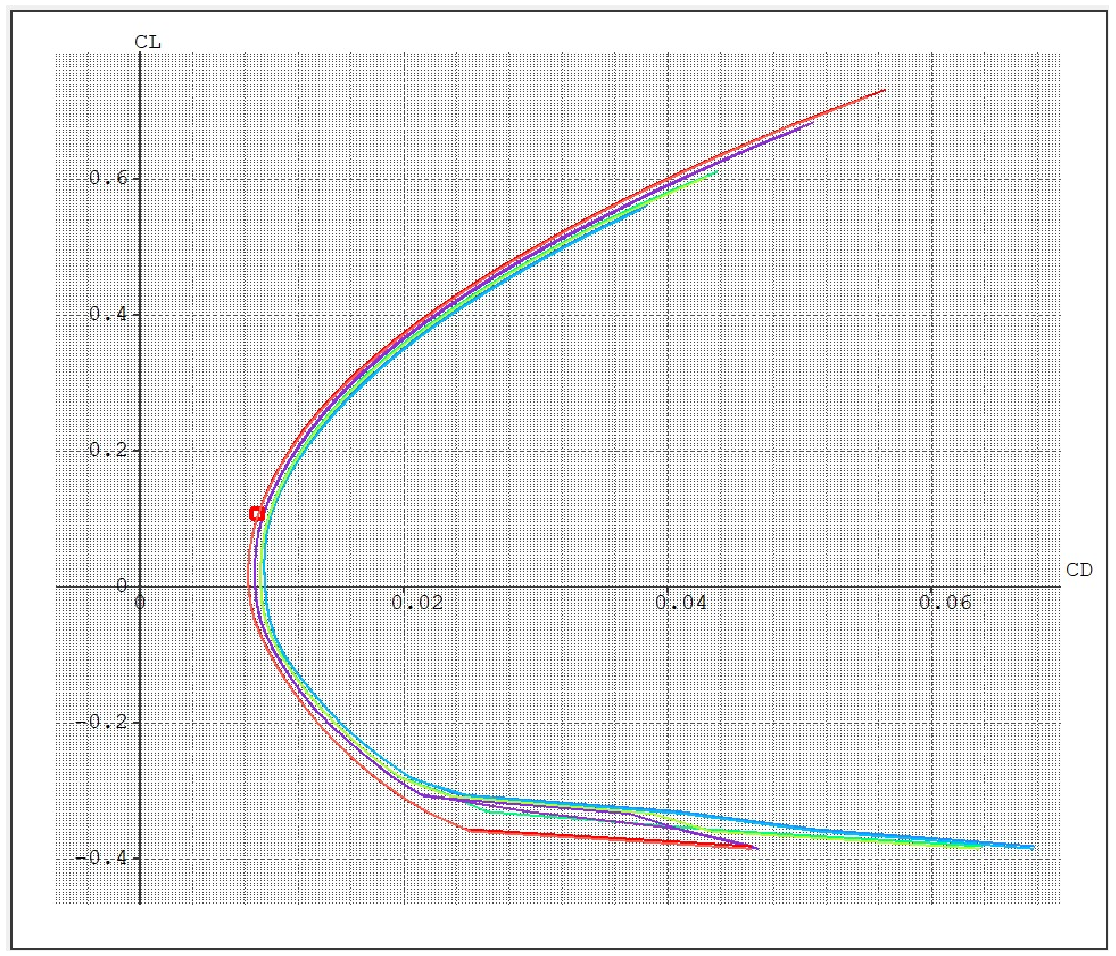
\includegraphics[scale=0.75]{Capitulo3/figs/cl y cd.pdf}
    \caption{EHEKALT BWB - polar ratio lift coefficient / drag coefficient}
    \label{razón polar coeficiente de lift / coeficiente de arrastre}
\end{figure}

The data in this chart are critical for aircraft pilots and designers, as they help determine the optimal flight profiles and control configurations to maximize aircraft efficiency and performance.

It is important to note that each aircraft has its own curve $C_L/C_D/\alpha$ specific, and this curve can change according to the configuration (flaps, slats, etc.) and flight conditions. Therefore, detailed tests and analyses are performed to determine these relationships in real conditions. For EHEKATL BWB and according to the Figures \ref{razón polar coeficiente de lift / coeficiente de arrastre} and \ref{EHEKALT BWB - Polar sustentacion arrastre ataque} it can be observed that the highest efficiency or best aerodynamic performance is given at high speeds. Although the lift coefficient showed a behavior just incremental as linear function, in the drag coefficient a difference was shown that we can consider significant and appreciable in a visual way, therefore, the curve of the most simulated speed $35 m/s$ shows the best performance in both functions. The ratio of increase of the lift coefficient to the drag coefficient begins at 3 to 1 considering a zero attack angle, around 12 to 1 with a equilibrium attack angle and maximum efficiency around 16 to 1 at the lowest speeds and 19 to 1 at the highest speeds, see Figure \ref{EHEKALT BWB - Polar sustentacion arrastre ataque}. 
\begin{figure}[!t]
    \centering
    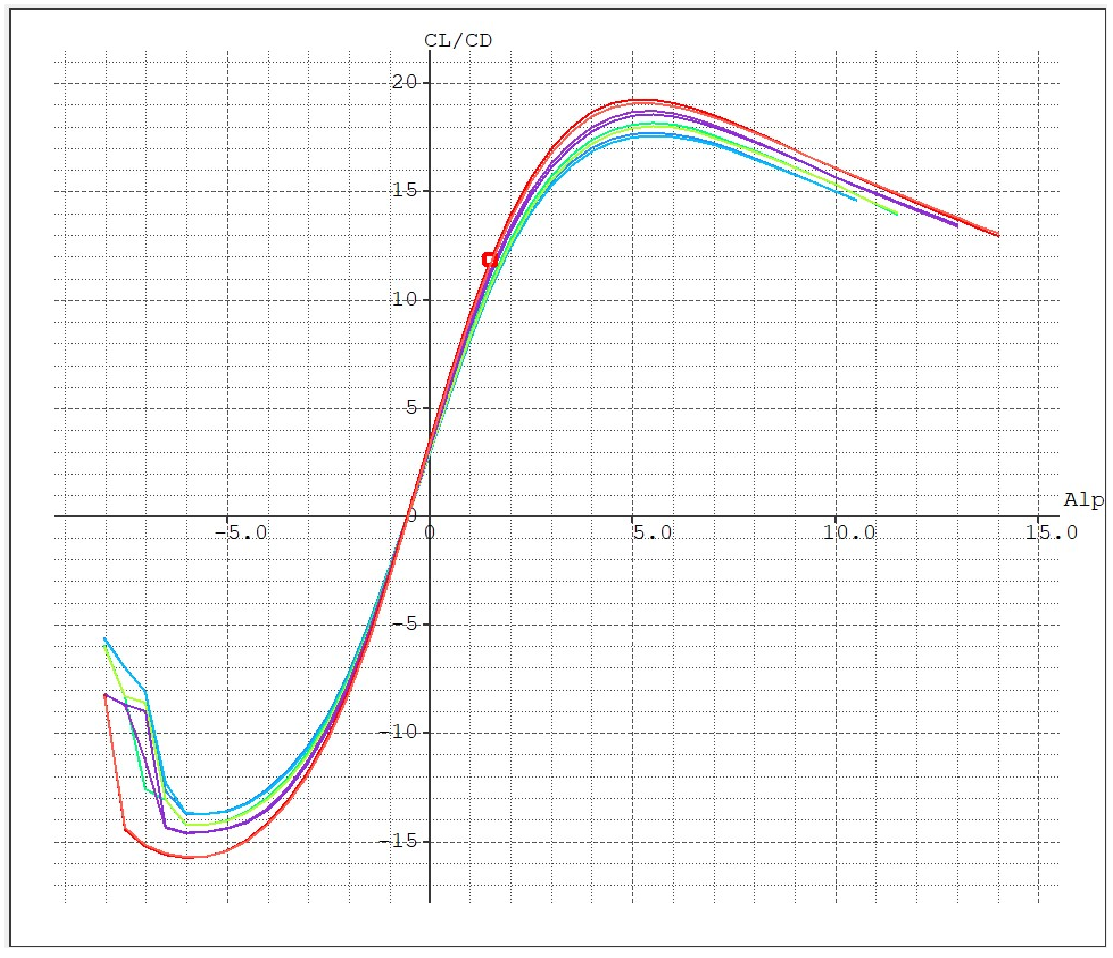
\includegraphics[scale=0.75]{Capitulo3/figs/cl cd.pdf}
    \caption{EHEKALT BWB - Polar support/trace with respect to the angle of attack}
    \label{EHEKALT BWB - Polar sustentacion arrastre ataque}
\end{figure}

\medskip

%%%%%%%%%%%%%%%%%%%%%%%%%%%%%%%%%%
\subsection{Stability Analysis with XFLR5}
In a normal flight it is usual for pilots to adjust the controls of the aircraft such that by releasing the controls the aircraft continues its flight in the desired flight condition. It is said that the aircraft was \textit{trimmed}, and \textit{trim} defines the initial condition where the variables of interest can be studied. \textit{trimming} This condition is fulfilled when the axial forces, normal and lateral; as the moments of roll, cabaceo and yaw are all zero. The balance of forces and moments is expressed in the requirements as lifting equal to weight. $L=W$ and push equal to drag $D=T$, this provides stability in the state of balance even after a disturbance generated by control inputs directed by the pilot or autopilot, or by external influences such as disturbances. 
\begin{figure}[!h]
\centering
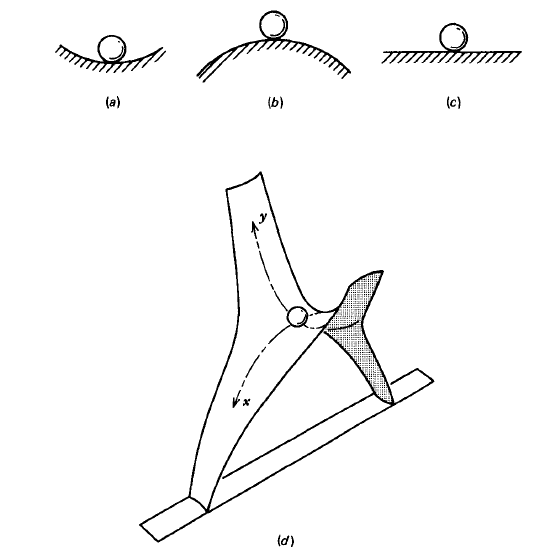
\includegraphics[scale=0.90]{Capitulo3/figs/4 22.png}
\caption{Balanced, stable and unstable ball \cite{Etkin1996}}
\label{fig: Bola en equilibrio, estable e inestable}
\end{figure}
To maintain a steady state, simultaneous adjustment of the main flight variables is required in the six degrees of freedom of the aircraft depending on the Mach number, the angle of the flight path, the geometric configuration of the aircraft, the weight and position of the centre of gravity. 
%
With variable parameters over time we have to adjust the balance during the flight as much as necessary. 
%
The typical aircraft symmetry confers aerodynamic properties that usually reduce the task to longitudinal adjustment only. Adjustment for lateral-directional balance is necessary when this aerodynamic symmetry is lost, which can occur when an engine in a multi-engine aircraft stops working, for example. 
%
A body is in balance if it is at rest or in uniform motion, that is, if it has constant linear and angular moments. 
%
In other words, the balance of an aircraft in uniform motion lacks rotation, i.e. a straight forward movement, since the aerodynamic forces are dependent on the angle of orientation of the aircraft with respect to the flight path, and because the resultant of these forces must balance accurately according to the weight and centre of gravity of the aircraft. 
%
The stability or lack of it, is a property of the states in balance. 
%
We speak of a stable state of equilibrium when the body (aircraft) is slightly disturbed in any of its degrees of freedom, and immediately returns to its initial state of equilibrium, \cite{Etkin1996}. 

The Figure is used \ref{fig: Bola en equilibrio, estable e inestable} to explain the neutral and unstable balance. 
%
The ball at the center of the geometry (d) is stable with respect to the direction $y$, but unstable if displaced in $x$. Aircraft comply with this principle, since they may be stable with respect to one degree of freedom, but unstable with respect to another. 
%
Two types of instability are relevant in the dynamics of an aircraft: \textbf{static instability} continuously separates the aircraft from its equilibrium condition, an example is ball in (b). \textbf{dynamic instability} is a complicated phenomenon where the aircraft oscillates around the state of equilibrium with a constant increase in its amplitude (not explicable with the figure \ref{fig: Bola en equilibrio, estable e inestable}).
%
When applying the concept of stability to the aircraft, two classes must be considered: \textbf{estabilidad inherente} is a basic property of aircraft geometry with its fixed or free controls. \textbf{synthetic stability} is the one that provides an Automatic Flight Control System (AFCS) and disappears if the control system fails. 
%
AFCS are capable of stabilizing inherently unstable aircraft, such as wing-integrated aircraft. It also improves their stability, the latter is known as \textbf{Increased Stability System (SAS)}The case of a SAS wing aircraft was shown in advance with NASA X-48 B/C. 
%
In an autopilot the closed loop system must stabilize in response the atmospheric disturbances and commands that come from the navigation system. 
%
Finally, the main roles played by a flight controller are the following: Set or change the equilibrium condition (speed or angle of ascent). An appropriate control must be able to produce a full range of the states of equilibrium where the aircraft can operate. Produce accelerated movements, or not states of non-balance, while maneuvers are carried out.

In short, the stability of an aircraft is divided into static stability and dynamic stability. 
%
The characteristics of static stability determine the \textit{trimmability} or adjustment to the balance of the aircraft. Static stability is commonly interpreted to describe the convergence trend given an initial equilibrium condition followed by a small disturbance towards this equilibrium condition.
%
Dynamic stability describes the transition movement in the process of regaining balance after a disturbance. 
%
To develop the stability analysis of EHEKATL BWB we will take the results obtained in simulation with XFLR5. 

\medskip
%%%%%%%%%%%%%%%%%%%%%%%%%%%%%%%%%%%%%%%%%%%%%%%%%%%%%%%%%%%%%%%%%%%%%%%%%
\textbf{Static stability of EHEKATL BWB}

Static stability can be explained with the Figure \ref{fig: Bola en equilibrio, estable e inestable}. The ball in (b) is \textbf{statically unstable} since after the forces and moments act on the body turns out to be a disturbance that the body cannot recover, and continually moves away from its state of equilibrium. Figure (a) is \textbf{statically stable} since after the forces and moments act in the body it tends to recover its state of equilibrium immediately. Figure (c) is \textbf{neutralmente estable} if the body is disturbed but the moment remains at zero and the body remains in balance. 
%
In the flight dynamics stability and instability are very important. It is very rare that neutral stability occurs in the flight dynamics of air vehicles. 

\medskip

%%%%%%%%%%%%%%%%%%%%%%%%%%%%%%%%%%%%%%%%%%%%%%%%%%%%%%%%%%%%%%%%%%%%%%%%%
\textbf{Longitudinal static stability}

The longitudinal static stability refers to the stability of the aircraft in the symmetric x-z plane and with respect to the pitching time. If an aircraft is longitudinally stable a small increase in the angle of attack will cause a change in the pitching time that will decrease the angle of attack. Otherwise, if there is a small decrease in the angle of attack then a change in the pitch time will be generated that will increase the angle of attack, \cite{Neubacher2008}.

The following equation shows the ratio of the pitching moment given an aircraft without impeneage (tailless aircraft), in a flight in quasi-stable equilibrium, with constant mass and for angles of small attacks. 
\begin{equation}
    C_m = C_{m0} - C_L (x_{cg} - x_{ac})
\end{equation}
The pitching moment is based on the lifting coefficient $C_L$, the difference in the distance from the centre of gravity to the aerodynamic centre $(x_{cg}-x_{ac})$ and the moment coefficient generated by wing characteristics $C_{m0}$. 
%
Of the most important restrictions on longitudinal static stability is that $M_w, M_q$ they must be negative, otherwise we would have static longitudinal instability, \cite{Neubacher2008}. 
%
The criteria for ensuring longitudinal static stability would then be as follows:
\begin{itemize}
    \item Negative slope in the function of the pitching moment $C_m$ with respect to the angle of attack $\alpha$
    \item Negative values in pitch moment coefficients relative to normal speed and pitch rate $M_w, M_q$ 
    \item Negative values in axial force coefficients relative to axial velocity and normal force relative to normal velocity $X_u, Z_w$
\end{itemize}
\begin{figure}[t]
    \centering
    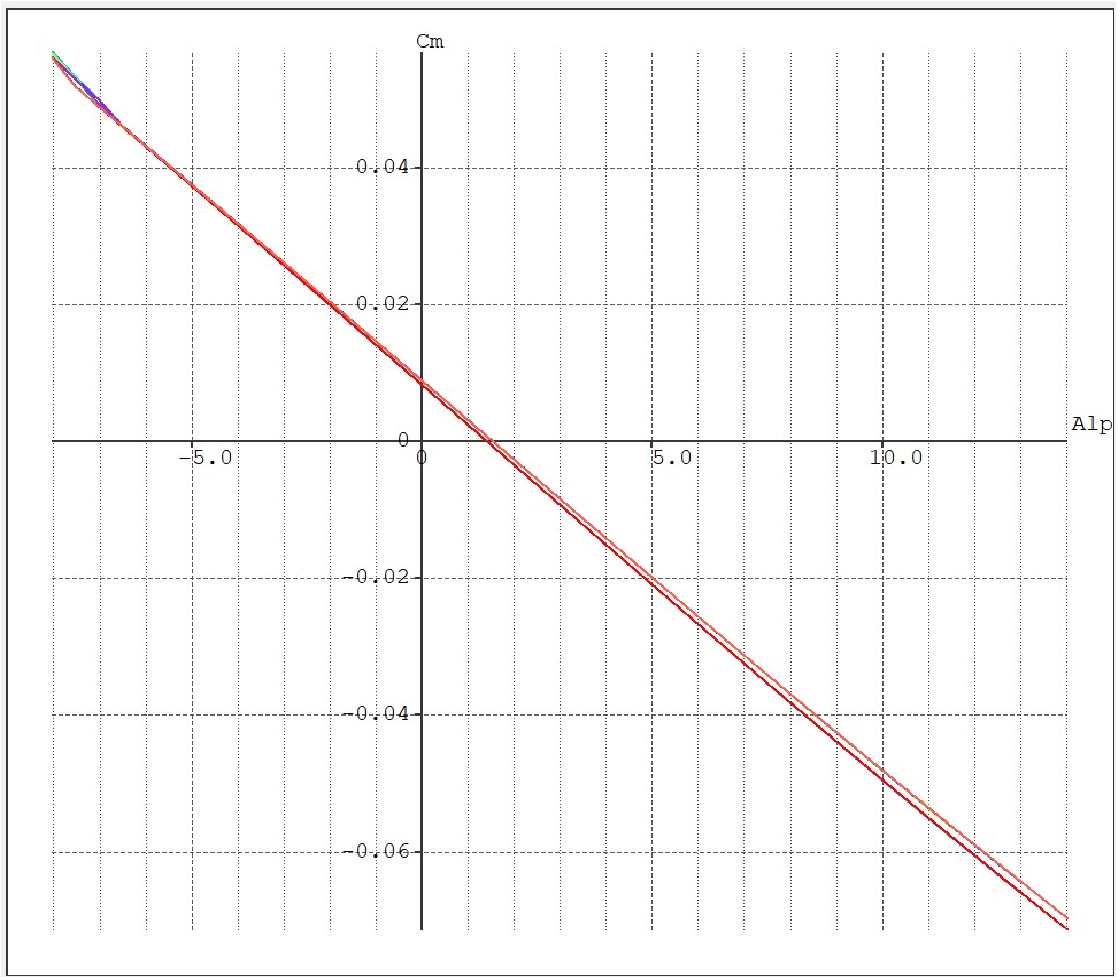
\includegraphics[scale = 0.65]{Capitulo3/figs/Cm a.pdf}
    \caption{Static stability in longitudinal dynamics}
    \label{Estabilidad estática en la dinámica longitudinal}
\end{figure}

Given the simulation results of the Figure \ref{Estabilidad estática en la dinámica longitudinal} the negative slope criterion for the $C_m$ with regard $\alpha$, ensuring longitudinal static stability. Negative value criteria for $M_w$,$M_q$ and $X_u$,$Z_w$ are also met. These values can be validated in the controller design chapter in the Table \ref{Coeficientes dimensionales longitudinales de EHEKATL BWB} and also in the Table \ref{Coeficientes dimensionales longitudinales de EHEKATL BWB adaptive}where they are used for EHEKATL BWB longitudinal control test simulations with PYTHON. 

\begin{figure}[!t]
    \centering
    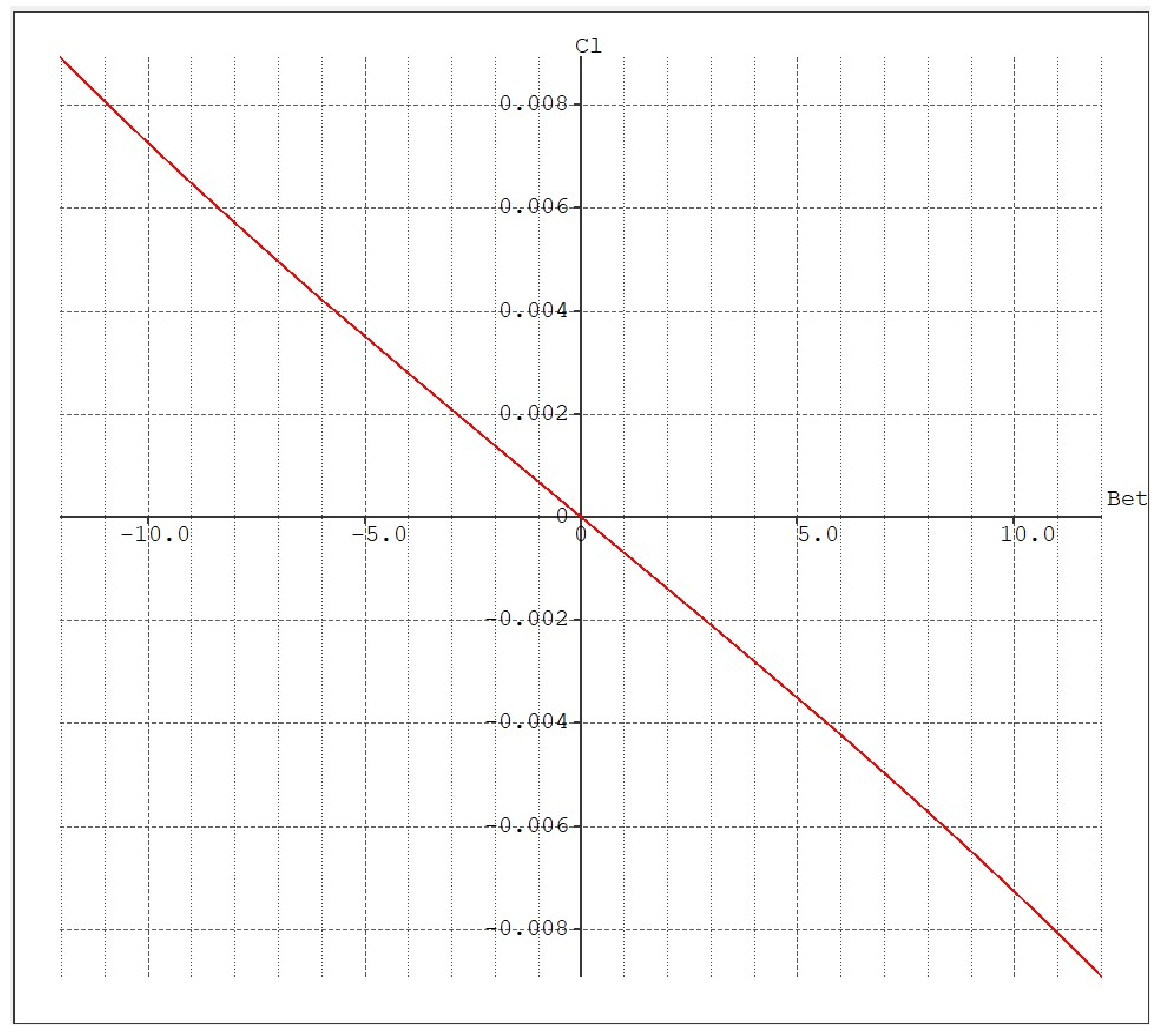
\includegraphics[scale = 0.66]{Capitulo3/figs/cl beta (2).pdf}
    \caption{Lateral static stability}
    \label{Estabilidad estática lateral}
\end{figure}


All stability simulations show the speeds used in the Table \ref{tab: Re y velocidades} The velocities are grouped into two functions according to the simulation type VLM1 and VLM2. The slightly steepest slope is VLM2. $\alpha$ for the moment of balancing is between 1.45$^\circ$ and 1.55$^\circ$. When the pitching time is zero it is essential to know the angle of attack, since at this point you can release the controls ensuring a straight and leveled flight. $\alpha$ in 1.5$^\circ$ as a specific value for later calculations.
%
Starting from the equilibrium point (value of $\alpha$ that does zero to $C_m$, in this case $\alpha$ of 1.5$^\circ$) it is observed that if the angle of attack decreases a positive moment is generated, and if the angle of attack increases a negative moment is generated. In a physical sense, if the aircraft is on a straight and level flight ($\alpha_e$ with $C_m = 0$) and a disturbance decreases or increases the angle of attack, the aircraft has the ability to recover the equilibrium condition after the disturbance. 

\begin{figure}[!t]
    \centering
    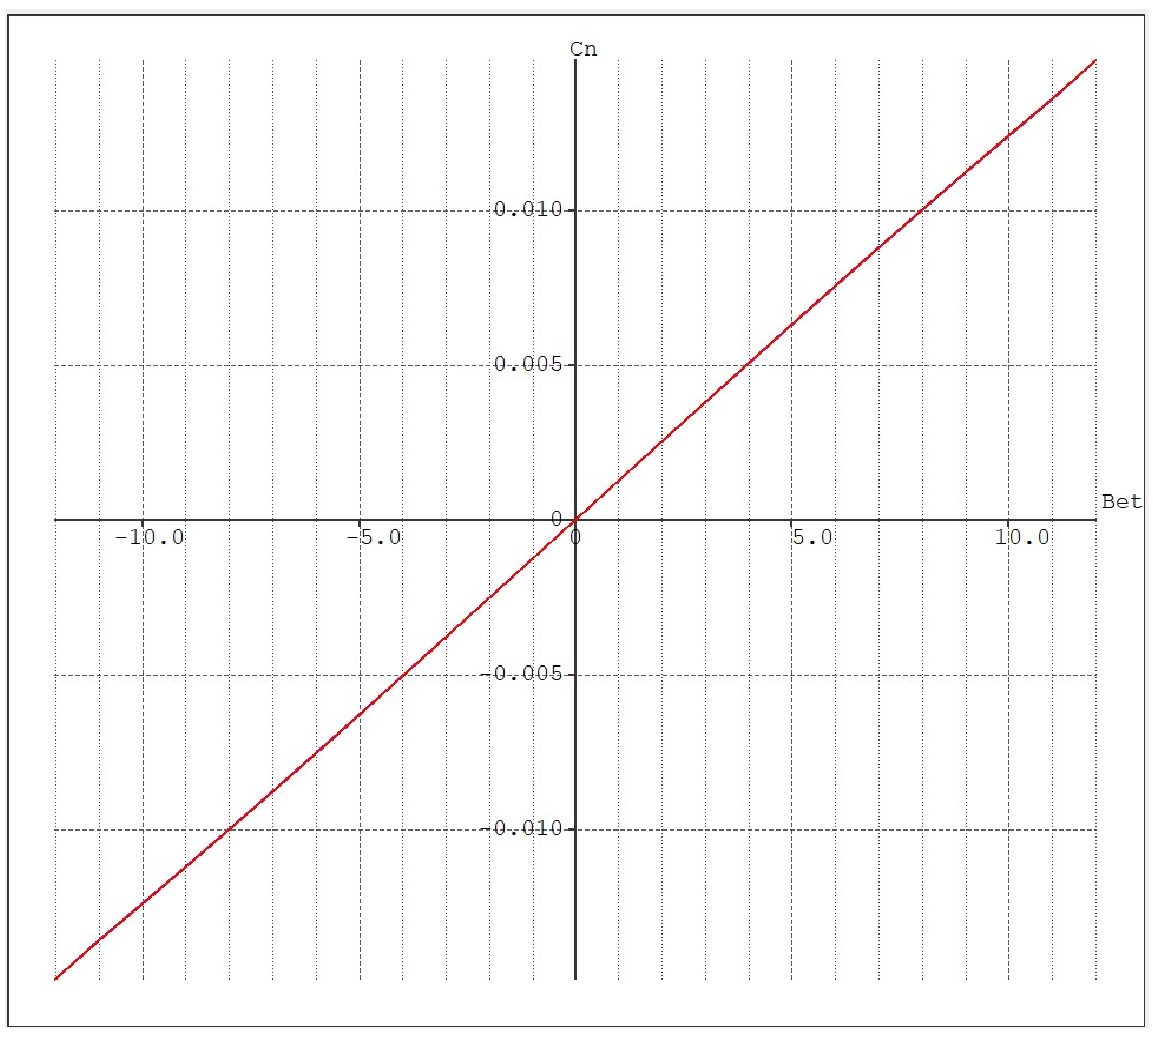
\includegraphics[scale = 0.65]{Capitulo3/figs/Cn beta (1).pdf}
    \caption{Directional static stability}
    \label{Estabilidad estática direccional}
\end{figure}


\medskip
%%%%%%%%%%%%%%%%%%%%%%%%%%%%%%%%%%%%%%%%%%%%%%%%%%%%%%%%%%%%%%%%%%%%%%%%
\textbf{Lateral-directional static stability}

According to \cite{Neubacher2008}, lateral static stability concerns the aircraft's ability to maintain a wing-level balance in the direction of wing action. 
%
The parameter with the greatest influence on lateral static stability is the diedro angle of the wing. 
%
The effect of the diedro in unempiaged aircraft configurations is equal to its implementation in conventional impeneage aircraft. 
%
Through the configuration of this parameter (diedro) we can design and adjust the lateral static stability according to the level of acceptability we are looking for. 

In order to ensure lateral static stability after a disturbance at the time of rolling, the following criteria are established:
\begin{itemize}
    \item Negative slope in the function of the rolling moment $C_l$ with respect to the sideslip angle $\beta$
    \item The value of the tipping moment with respect to the sideslip angle $L_\beta$ must be negative
    \item  The value of the rolling moment with respect to the angle speed of rolling $L_p$ must be negative
    \item The value of the lateral force coefficient relative to the sideslip angle $Y_{\beta}$ must be negative
\end{itemize}

Directional static stability treats aircraft stability on the shaft $z$. It is sought that the aircraft can return to the condition of equilibrium after experiencing a disturbance at the moment of yawing. To ensure that the aircraft regains stability we must meet the following criteria:
\begin{itemize}
    \item Positive pending at yaw time $C_n$ with respect to the sideslip angle $\beta$
    \item The value of the yaw moment coefficient with respect to the sideslip angle $N_\beta$ must be positive
\end{itemize}

According to the simulation results of Figures \ref{Estabilidad estática lateral} and \ref{Estabilidad estática direccional} the static stability criterion with negative slope is met $C_l$ concerning $\beta$ for lateral stability and positive slope in $C_n$ concerning $\beta$ for directional stability. Similarly, the criteria of negative values in the coefficients are met $L_\beta$,$L_p$,$Y_{\beta}$ for lateral stability and positive value in coefficient $N_\beta$ for directional stability. Such values can be validated in the controller design chapter in the Table \ref{Coeficientes dimensionales laterales de EHEKATL BWB}where they were used to perform the lateral-directional control simulations of EHEKATL BWB in PYTHON. 

%%%%%%%%%%%%%%%%%%%%%%%%%%%%%%%%%%%%%%%%%%%%%%%%%%%%%%%
\section{EHEKATL BWB design at Plane Maker}


Plane Maker is a program used in the development of the X-PLANE flight simulator. It is known for its realism in flight dynamics and is used by aviation professionals, amateurs and flight enthusiasts for training and research. Plane Maker is a graphical user interface (GUI) that allows users to create and modify aircraft models within the X-PLANE environment. It provides a platform to design and customize various aspects of an aircraft, including its geometry, aerodynamics, weight and balance, systems and performance features.

For the geometric design of EHEKATL BWB a total of 20 wing sections were configured, including fins and vertical stabilizers, see Figure \ref{Diseño Aerodinámico de EHEKATL BWB en Plane Maker}. The sections were numbered in the same order as Plane Maker, and correspond to the previous design in XLR5. The parameterization in Plane Maker is particular. In the block shown below the geometric design of EHEKATL BWB in Figure \ref{Diseño Aerodinámico de EHEKATL BWB en Plane Maker} The parameterization or specifications of the number one wing section (1), corresponding to the half-left in the central section of the body of EHEKATL BWB, is seen. Using this section number one as an example, the first parameter is the distance from the root profile (attached to No. 11) to the tip profile (along with No. 2) called \textit{semi-length} or semi-wing. This distance is not considered as in XLR5, where it is a linear distance (on the axis $y$) and easy to parameterize with respect to the fret. In Plane Maker it is considered distance from 25$\%$ To be able to work this new design according to the requirements of Plane Maker, a code is developed in PYTHON that extrapolates the parameters of the design of EHEKATL BWB in XFLR5 to adapt it to the fields of Plane Maker considering the change of units from the international system to the English system. Such code can be reviewed in the GitHub account of the the thesis author. The link is in the appendices section. \ref{a codigos python}. Later, in the same block of the Figure \ref{Diseño Aerodinámico de EHEKATL BWB en Plane Maker} you have the adjustment for the root profile string (\textit{root chord}) and the rope of the tip profile (\textit{tip chord}). Then, in the central part of this same block the arrow angle and the diedro angle are adjusted, as well as the section of the semi-wing being designed, left or right. Finally, the coordinates of the semi-wing section on the three axes are adjusted: \textit{long arm} for distance in $x$, \textit{lat arm} for distance in $y$ and \textit{vert arm} for distance in $z$. The sections of the semi-left wing 2 and 4, and of the semi-right wing 12 and 14 were respected according to the previous design in XFLR5. In XFLR5 these sections were designed to be able to design the ACS with the geometry established at the leak edge. EHEKATL BWB's design was respected in Plane Maker to have exactly the same model proposed in the previous sections. 

\begin{figure}[!t]
    \centering
    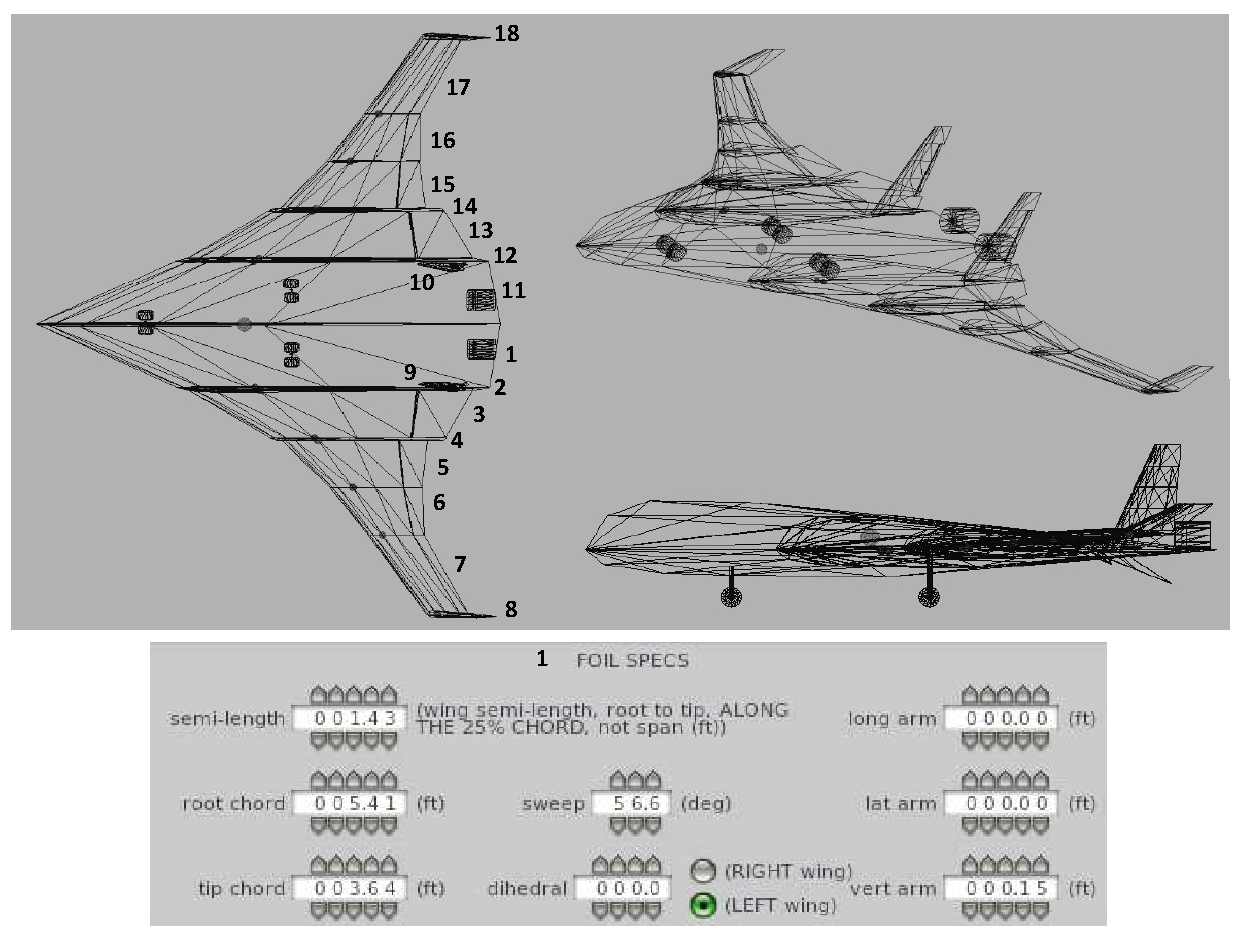
\includegraphics[scale=0.62]{Capitulo3/figs/Diseño EHEKATL BWB Plane Maker 2 (1).pdf}
    \caption{EHEKATL BWB aircraft design at Plane Maker}
    \label{Diseño Aerodinámico de EHEKATL BWB en Plane Maker}
\end{figure}

The configuration of the aerodynamic control surfaces of EHEKATL BWB are found in Figure \ref{Dimensión de las ACS de EHEKATL BWB}. The ACS were dimensioned in the same way as in XLR5. \ref{Dimensión de las ACS de EHEKATL BWB} there are two first columns (from left to right) where the name of the ACS to be dimensioned and the legend comes \textit{chord ratio} which alludes to the percentage of rope that is considered for the control surface, from the trailing edge to the attack edge. The first column is for the percentage relative to the root rope, and the second regarding the tip rope. 
\textbf{EHEKATL BWB has two pairs of lifts, two pairs of wingers and a pair of steering rudders}. When the legend is observed \textit{aileron 1} corresponds, for example, to the pair of wings located in the section of the left half-wing no. 7 and the section of the right half-wing no. 17. This same principle applies to elevators but not so for steering rudders, where it refers to each element and not its pair. All ACS were dimensioned to a 20$\%$ both the root profile and the tip profile.Also, the deflection of all the ACS is set in $-30/+30$. This parameterization is seen in the following two columns of the Figure \ref{Dimensión de las ACS de EHEKATL BWB}, where the first corresponds to downward deflection and the second to upward deflection. Finally, the ACS were configured as \textit{Smooth with no loops}, which translates as smooth and without gaps, or smooth without spaces. This parameterization allows to appreciate the leak edge as the only geometry if no ACS has deflection. 

\begin{figure}[!t]
    \centering
    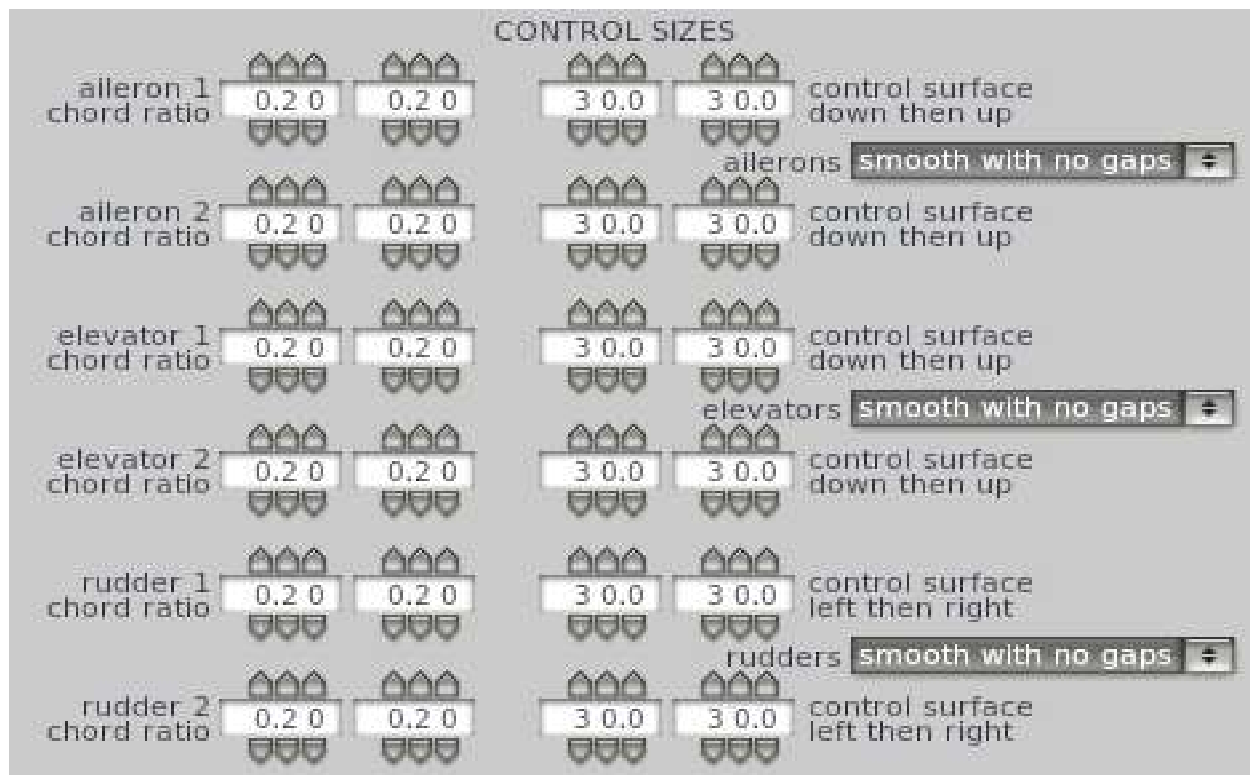
\includegraphics[scale=0.5]{Capitulo3/figs/ACS plane maker.pdf}
    \caption{Dimension of EHEKATL BWB ACS in Plane Maker}
    \label{Dimensión de las ACS de EHEKATL BWB}
\end{figure}

Once the geometric design and ACS of the EHEKATL BWB aircraft is defined in Plane Maker, the MH78 and MH80 profiles designed in Airfoil Maker, in addition to the NACA 0009 already in the program, must be implemented. The MH80 profile is implemented in the central section where the payload and the various avionic components are located and is limited to where the section is finished with the first ACS, or main elevators. The rest of the wing is MH78 profile except the fin that is NACA 0009 together with the vertical stabilizers. \ref{Implementación de perfiles de EHEKATL BWB} the implementation of the profiles in the right half-wing and vertical stabilizers is observed. In addition, the Clark-Y profile is established for the propellers or propellers of the engines. 
%
\begin{figure}[!t]
    \centering
    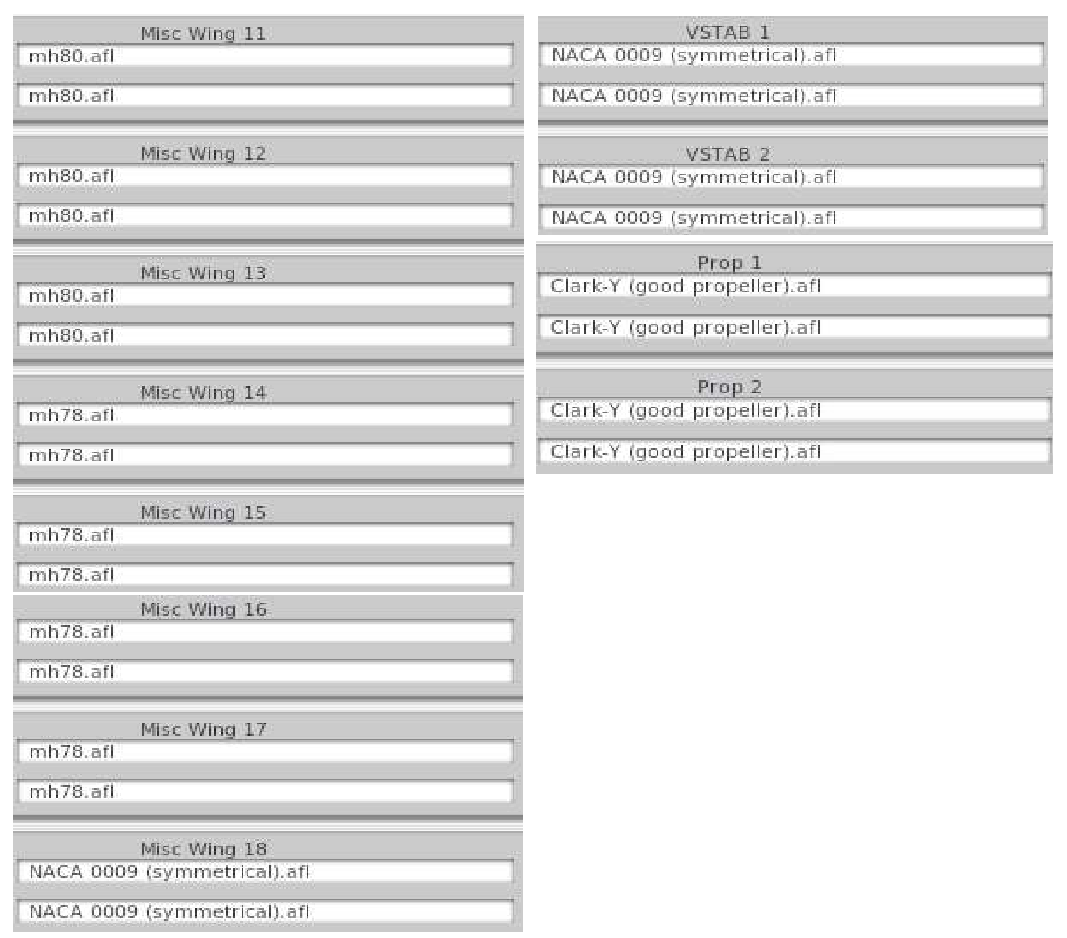
\includegraphics[scale=0.7]{Capitulo3/figs/perfiles plane maker.pdf}
    \caption{Implementation of profiles MH78,MH80 and NACA 0009 for EHEKATL BWB in Plane Maker}
    \label{Implementación de perfiles de EHEKATL BWB}
\end{figure}
%


In the Figure \ref{Especificaciones de motores} The specifications of the engines are shown. Since in X-PLANE the Jet engines consider a combustion chamber, and then, a higher thrust capacity for aircraft applications on a real scale, the engines selected for EHEKATL BWB are ductofan engines consisting of a fan within a pipeline energized by electric batteries. Clark-Y profiles apply in this geometry of the fan propellers within the ducts. 
 
\begin{figure}[!t]
    \centering
    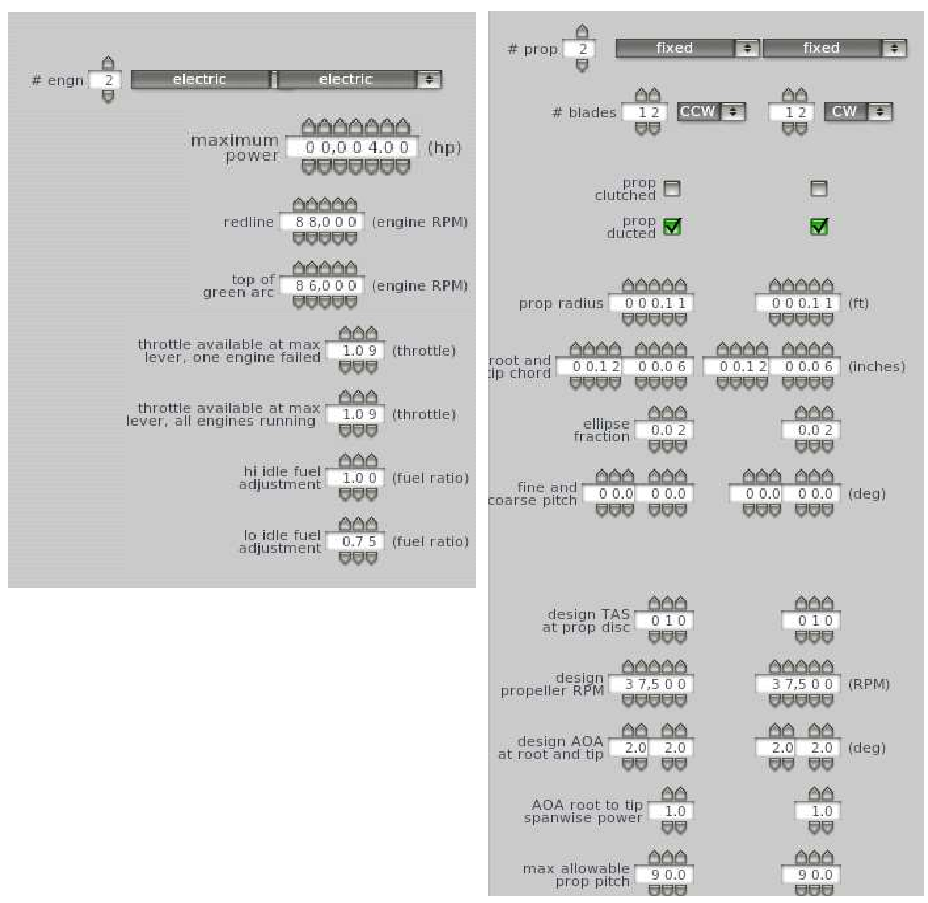
\includegraphics[scale=0.7]{Capitulo3/figs/espf motores.pdf}
    \caption{Engine specifications}
    \label{Especificaciones de motores}
\end{figure}
In the figure \ref{Especificaciones de motores} The main configurations of the electric motors and propellers or propellers are observed. The parametrization of the propulsion system is explained below. 
\begin{itemize}
    \item Two electric motors are selected. 
    \item The maximum power of both electric motors is set at 4hp, i.e. each engine offers 2hp or 1491.4 watts(W). An efficiency of 90 is considered in application.$\%$. 
    \item The maximum engine speeds are set at 88,000RPM and an available acceleration of 1.09 indicates 100$\%$ of the acceleration capacity.
    \item It establishes the reason or adjustment of fuel or energy, which refers to the process of configuring the amount of energy (in the case of our electric battery) that releases the power source to the engine during high and low operating speeds. For high speeds a ratio of 1 and for low speeds a ratio of 0.75 is established. 
\end{itemize}

Now let's explain the second block of the Figure. \ref{Especificaciones de motores} corresponding to the specifications of fan propellers within the ducts. 
\begin{itemize}
    \item Two fixed fans (one for each engine) are selected.
    \item 12 propellers were placed. The radius of the propellers is set at approximately 0.11ft or 33.5mm. This consideration is for ductofan engines around 70mm in diameter, where also 80mm and 90mm are common.
\end{itemize}
  
In addition to the characteristics of the motors and propellers that make up the fan within the duct, the characteristics of the electrical system are fundamental in the development of a VANT. The electrical system is configured with the two electric batteries proposed in the section \ref{superficie alar y potencia requerida}where each battery offers 0.146 watt-hour, and the generator design has a ratio of 0.25 RPM. 


In the Figure \ref{Centro de gravedad y peso de EHEKATL BWB} The location of the centre of gravity, the maximum and empty mass and the parameterization of the landing gear are shown. 
\begin{figure}[!t]
    \centering
    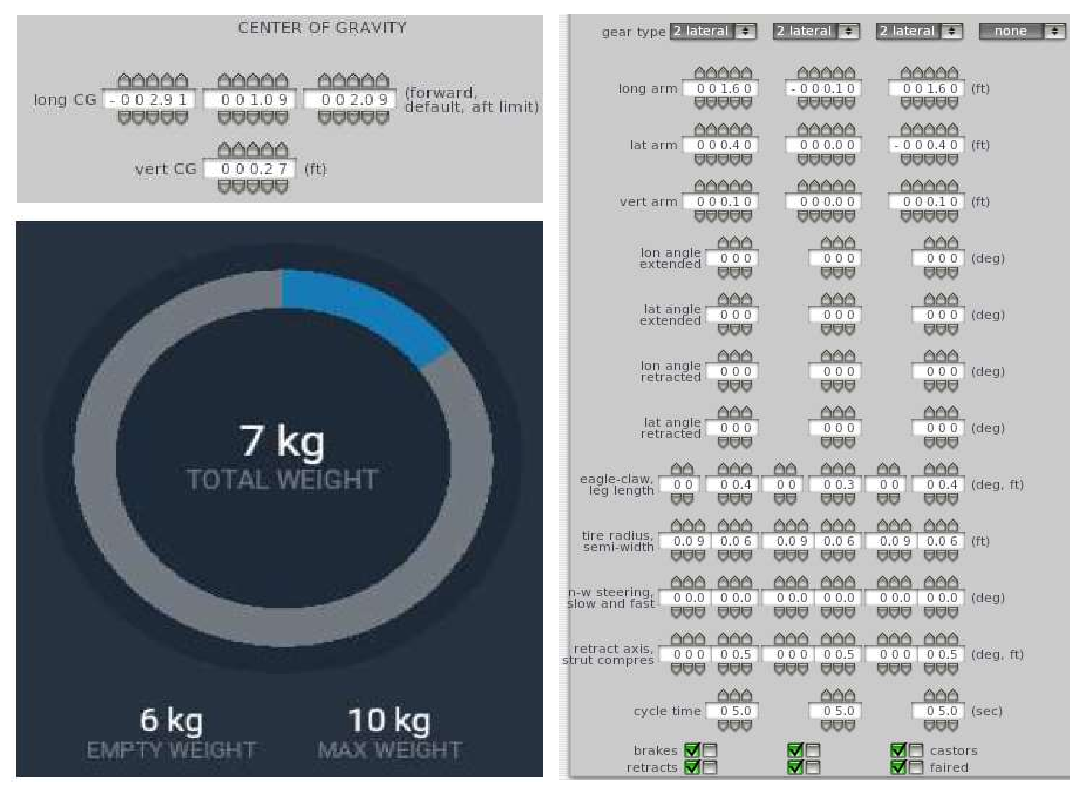
\includegraphics[scale=0.7]{Capitulo3/figs/weight and landing gear.pdf}
    \caption{EHEKATL BWB Gravity and Weight Center}
    \label{Centro de gravedad y peso de EHEKATL BWB}
\end{figure}
In the Figure \ref{Centro de gravedad y peso de EHEKATL BWB} The coordinates of the centre of gravity are set and just below the empty mass and the maximum mass. The empty mass is set at 6kg but rather as the minimum mass of EHEKATL BWB, and 10kg as effectively as the maximum mass. The mass of 7kg is set for simulation purposes. Finally, the landing gear is set. Three landing gear systems are selected. From left to right, the first column configures the rear train on the left side, the second the central front train close to the nose and the third train also rear but right side. Double wheel landing trains are set up. In the next three rows the location coordinates for each train are set up. \textit{eagle-claw, leg length} which refers to the length of the train leg when it is extended. \textit{tire radius} corresponding to the radius of the rim and \textit{semi-with} which corresponds to the semi-width of the same rim. Finally, the specifications for the retractable system are adjusted, where \textit{retract axis, strut compres} refers to the amount of compression of the train leg during the retracting cycle. A five-second retracting cycle is established, and in the final part of the block the retractable option with brake system is selected. 


In the panel of the cab EHEKATL BWB 26 navigation instruments were implemented, see Figure \ref{Panel de Cabina de EHEKATL BWB}Each instrument and its use are listed below.

1) Brake indicator. Turn on the word red \textit{brake} 2) Mach. Similarly it shows the speed according to Mach. 3) Incline or slip level. The bubble exits from the center with respect to the wing lateral inclination. 4) Indicator of collapse. Indicates when the aircraft is in a loss situation (out of control). 5) Engine power indicator. Shows in $hp$ 6) Loss from the angle of attack. It indicates radially when it is at a stable angle of attack and when it transcends an angle of attack that causes collapse. 7) Angle of attack at landing. It indicates by means of three lights whether the aircraft must maintain, raise or lower the angle of attack for a soft landing. 8) Indicator of the angle of attack. It shows the angle of attack linearly in degrees. 9) Window of horizon. It shows the line of horizon and inclination of the wing and of the nose regarding this one in degrees. 10) Indicator of the speed of the air. It indicates linearly the speed of the air in nodes. 11) Ascent speed. Vertical or ascent speed shown in linear way and in degrees. 12) Altimeter. It indicates the height regarding the level of the sea in feet. 13) Altimeter.Indicates the height with respect to ground by means of a rada en pies. 14) Indicator of the sideslip angle. Indicates the angle of drift in degrees. 15) Compas. Older instrument of navigation. 
\begin{figure}[!t]
    \centering
    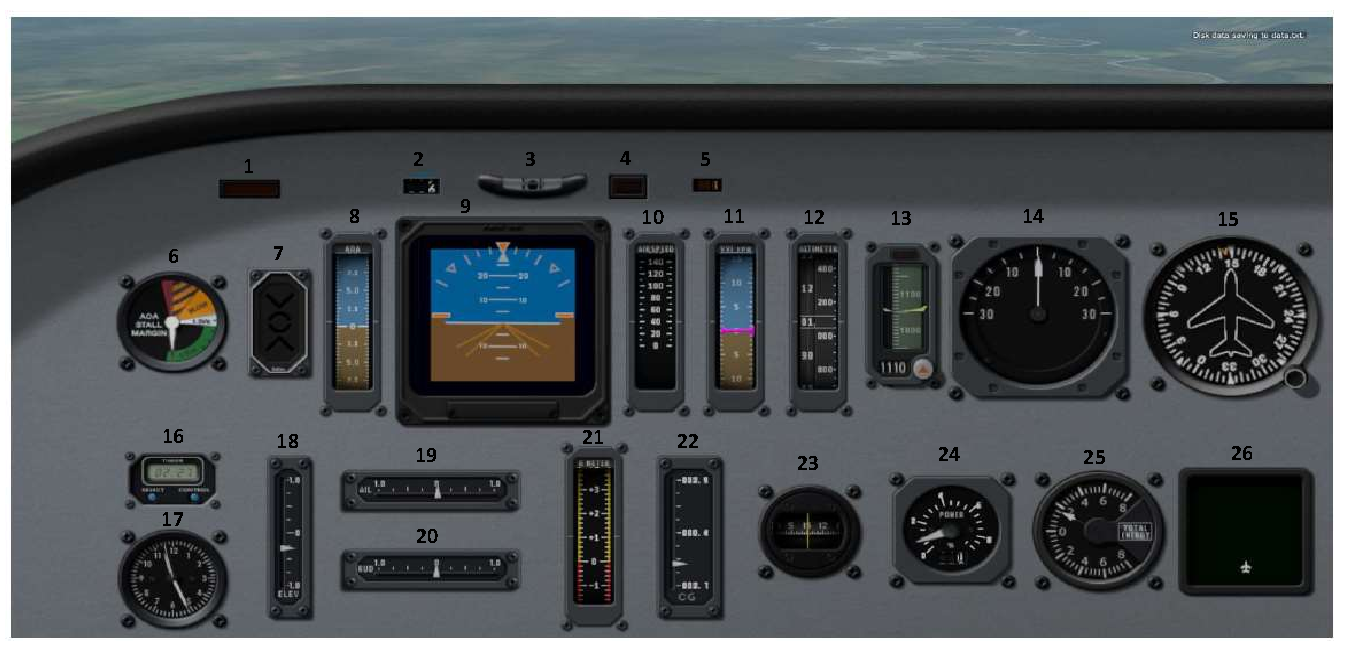
\includegraphics[scale=0.6]{Capitulo3/figs/paneles ehekatl 2.pdf}
    \caption{EHEKATL BWB Cabin Panel}
    \label{Panel de Cabina de EHEKATL BWB}
\end{figure}
16) Chronometer. Measure flight time. 17) Clock. Simple analog clock. 18) Elevator deflection indicator. Indicates the deflection of the elevators on a scale of 1 to -1, with zero deflection. 19) Aileon deflection indicator. 20) Tire deflection indicator. 21) Forces G. Linear indicator of forces G. 22) Gravity centre. Lineal indicator of the position of the center of gravity. 23) Compas. Similar to the previous one but with a linear design instead of radial. 24) Power indicator. Shows the power of the engines. 25) Displays the total potential and kinetic energy of the aircraft. 26) Radar. Displays near aerial vehicles in green color. 

While EHEKATL BWB is thinking to be a VANT, the same instrumentation can be monitored in real time in a ground system.

\begin{figure}[!t]
    \centering
    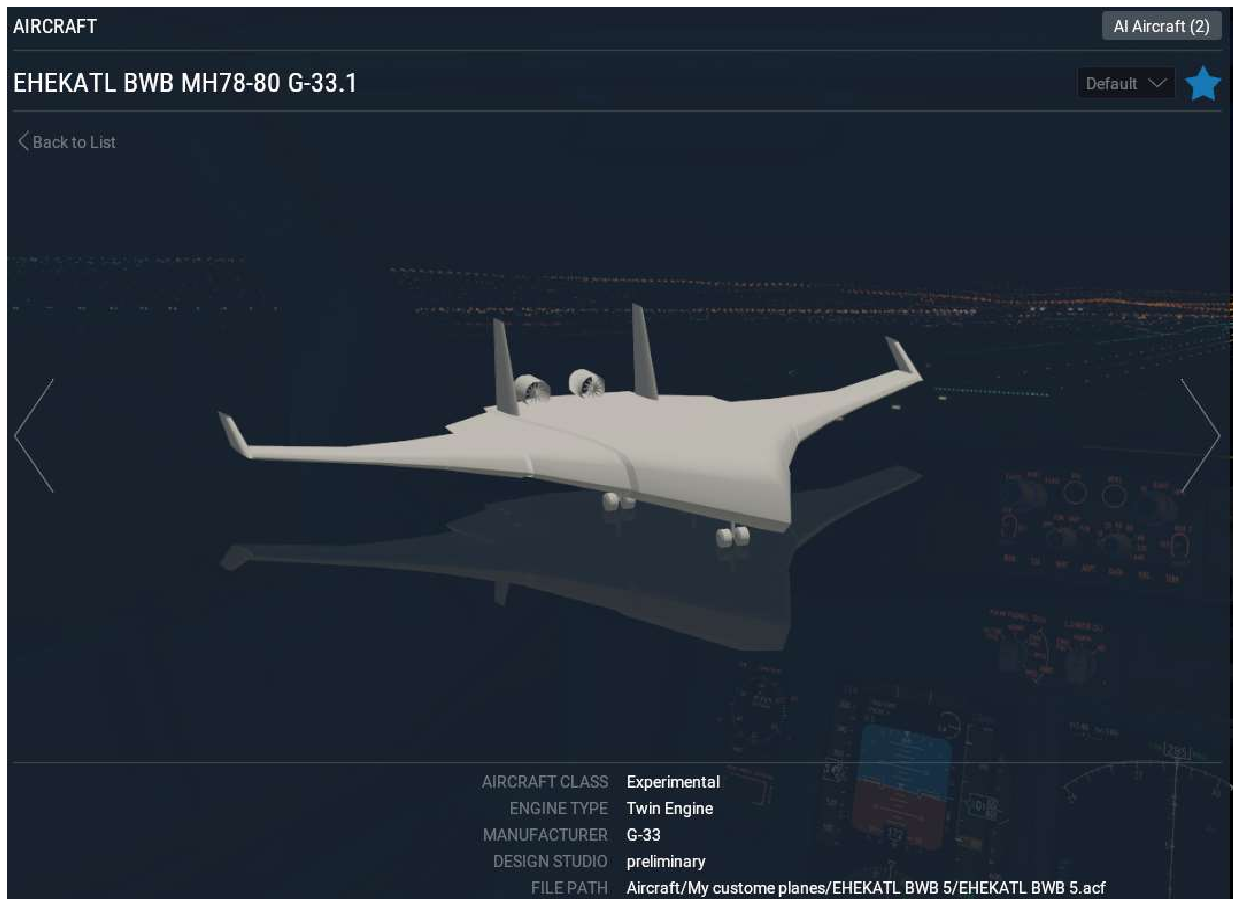
\includegraphics[scale=0.66]{Capitulo3/figs/Datos generales.pdf}
    \caption{EHEKATL BWB in the X-PLANE flight simulator environment}
    \label{Datos generales de EHEKATL BWB G-33}
\end{figure}

In the Figure \ref{Datos generales de EHEKATL BWB G-33} the final model of EHEKATL BWB performed in Plane Maker is observed within the environment of the X-PLANE flight simulator. 

\section{Discussion}

The clear and precise definition of the flight mission is a fundamental step in the design of any aircraft. Using the international standard atmosphere is a good first approximation to determine the pressure, density and temperature of the air depending on the altitude where the flight mission is planned. 

The selection and analysis of aerodynamic profiles in XFLR5 allows a detailed assessment of the aircraft's bearing and strength characteristics. The choice of profiles for BWB aircraft is crucial, where in addition to looking for good aerodynamic performance you need to consider pitch stability. 

Airfoil Maker's aerodynamic profile design process complements the XFLR5 assessment. Achieving the same behavior between XFLR5 results and Airfoil Maker design is essential to achieve a subsequent Plane Maker consistent design and X-PLANE simulations with good approximations. 

The XFLR5 application for aerodynamic analysis provides valuable information on the distribution of pressure and flow around the aircraft. This analysis contributes to the detailed understanding of the aerodynamic behavior of the EHEKATL BWB and allows for design adjustments to improve performance.

The evaluation of the stability and control of EHEKATL BWB in XLR5 is a critical step to ensure manoeuvrability and safety during flight. The results of this analysis influence the configuration of control surfaces and stabilization systems.

The implementation of the conceptual design in Plane Maker represents a significant milestone in the aircraft's development process. This stage allows the translation of theoretical concepts and aerodynamic data into a functional virtual model, which facilitates flight simulation and testing.

The detailed review of the design steps presented in this chapter provides a basis for the practical implementation and refinement of the aircraft of EHEKATL BWB. The results of the aerodynamic and stability analyses influence the design decisions and the final configuration of the aircraft, recalling the iterative process in aircraft design. 















%%%%%%%%%%%%%%%%%%%%%%%%%%%%%%%%%%%%%%%%%%%%%%%%%%%%%%%%%%%%%%%%%%%%%%%%
%           Capítulo 3: Modelado de la Aeronave               %
%%%%%%%%%%%%%%%%%%%%%%%%%%%%%%%%%%%%%%%%%%%%%%%%%%%%%%%%%%%%%%%%%%%%%%%%%
\chapter{Dynamic Modeling}

Once the aerodynamic design is completed, this chapter presents the dynamic model of EHEKATL BWB. Since aircraft are considered complex dynamic systems during their flight operation and are not stable by themselves, they need a control system to fly in the desired direction and compensate for disturbances.
%
 For the dynamic modeling of EHEKATL BWB we will consider a rigid body of six degrees of freedom; three degrees of displacement (towards, to one side and downwards) and three degrees of rotation (to top, to roll and yaw). Thus, we will have six differential equations, based on Newtonian laws, that will govern the movement of the aircraft. 
%
For the development of the dynamic model EHEKATL BWB is proposed with two engines, eight aerodynamic control surfaces on the trailing edge and two directional rudders on the vertical stabilizers.
%
In \ref{modelado TVC}, the modeling for EHEKATL BWB TVC is proposed considering a nozzle with deflection for generation of pitching and yawing moments. 
  
%%%%%%%%%%%%%%%%%%%%%%%%%%%%%%%%%%%%%%%%%%%%%%%%%%%%%%%%%%%%%%%%
\section{Reference Systems}
%%%%%%%%%%%%%%%%%%%%%%%%%%%%%%%%%%%%%%%%%%%%%%%%%%%%%%%%%%%%%%%%

A \textbf{Inertial Reference System} is a field where Newton’s second dynamic law is fulfilled. We can say that the variation at the linear and/or angular moment of the system is equal to the actual forces acting on the system, meaning that the system is considered at rest or in relative motion uniform at least that an external force acts on it. \textbf{Non-Inertial Reference System} It is the one with respect to an inertial system that is moving with acceleration, in this field the laws of Newton are not fulfilled. In a Non-Inertial System it is necessary to introduce the term fictitious forces (some fictitious forces may be the force of Coriolis or the centrifugal force).
%
The \textbf{terrestrial reference systems} which are used are: 
\begin{itemize}
    \item Centro-Terrestre Inercial $(i)$
    \item Centro-Terrestre Fijo $(e)$
    \item Local Geodesic $(\lambda, \phi, h)$
\end{itemize}
The Fixed Center-Terrestrial Reference System (ECEF), also known as the Geocentric Reference System, rotates at the Earth's real speed with respect to the Inertial Center-Terrestrial Reference System (ECI), which represents the non-rotational inertial coordinate axes. $(i)$ while ECEF by $(e)$. Both are orthogonal and have their origin in the center of the earth. $z_{i,e}$ are aligned as a fixed axis to the Earth rotation vector, while $x_{i,e}, y_{i,e}$ are located in the equatorial plane, with $x_i$ fixed in some direction with celestial reference, for example, a line connecting to the center of the sun regarding the position of the earth in spring equinox. $x_e$ usually intersects with the Greenwich meridian at equator level, where the axis $y_e$ completes the system of the right hand. The definition of the ECEF may vary, but the rule of two vectors should always be followed in the direction of the Earth rotation, see Figure \ref{Sistemas de Referencia Terrestres}.
  
\begin{figure}[!t]
\centering
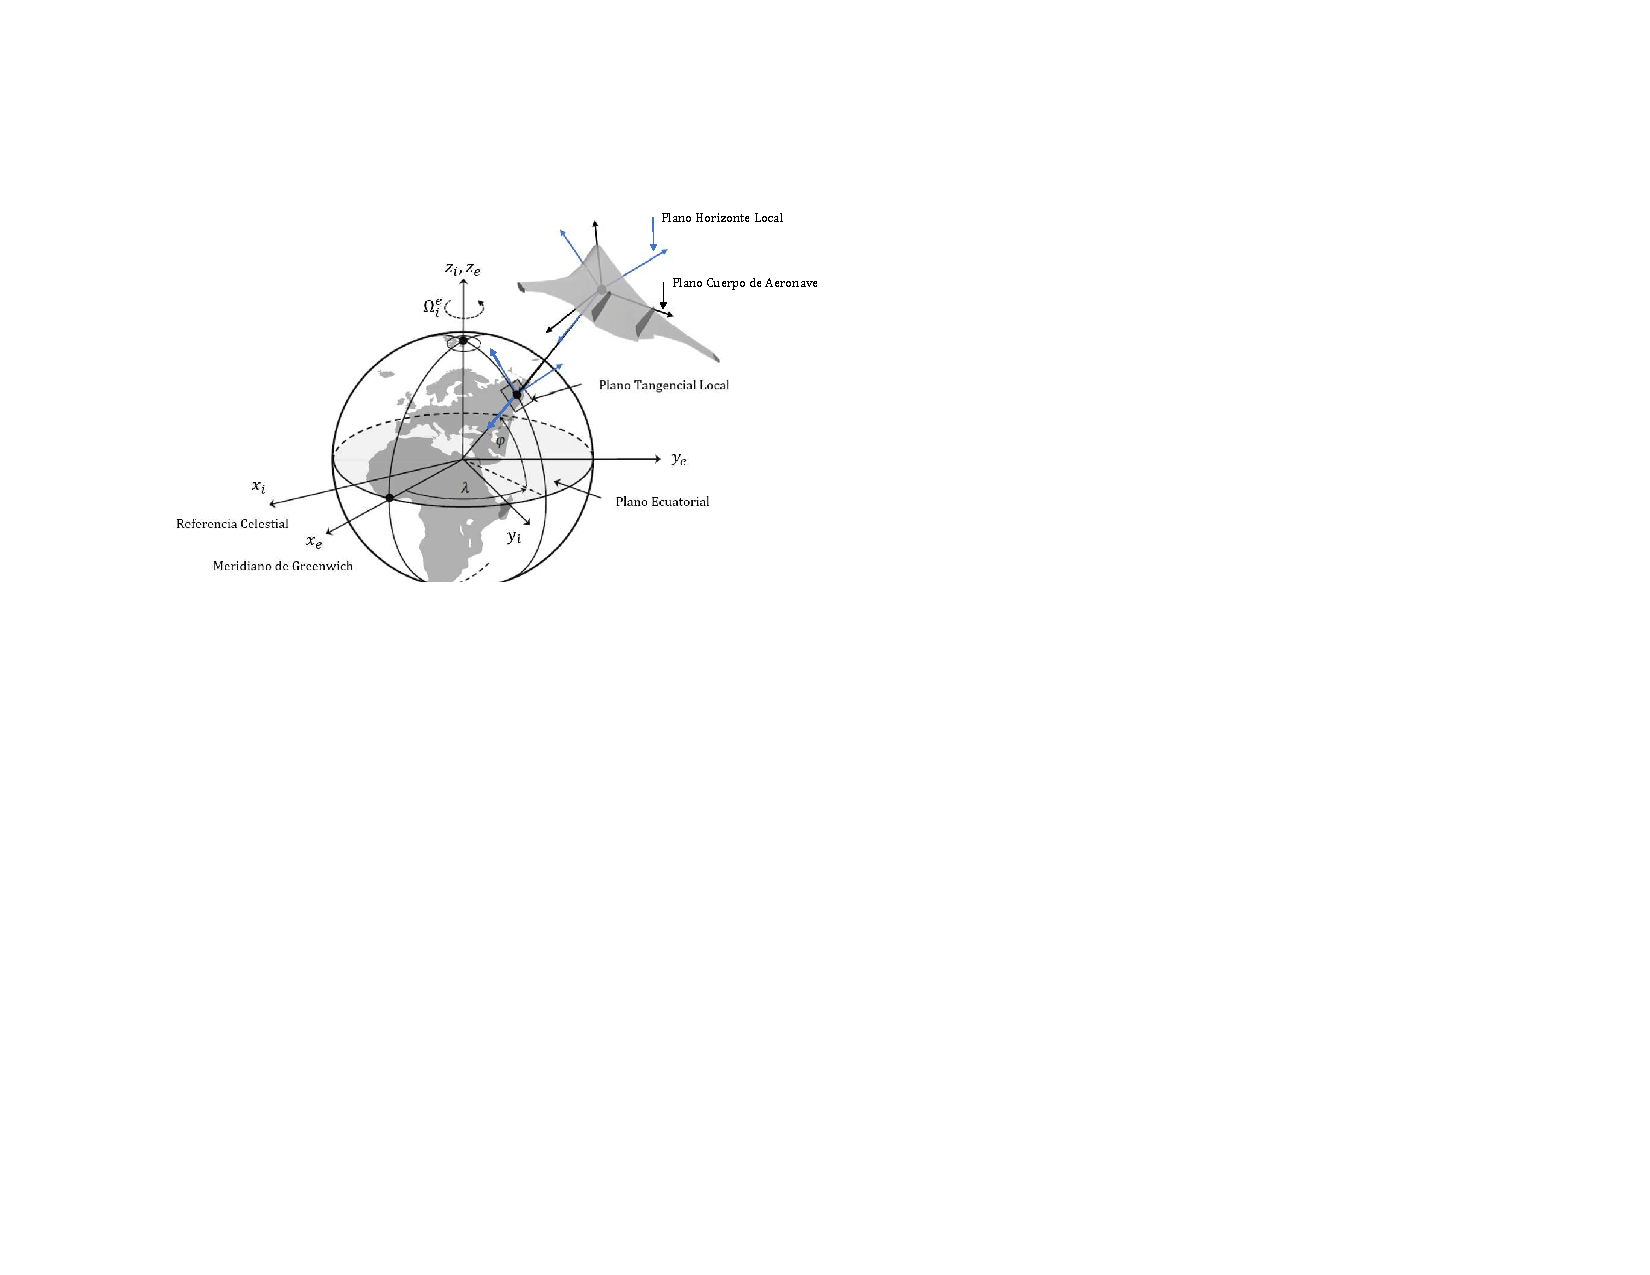
\includegraphics[scale=1.22]{Capitulo3/figs/Sistema de referencia Full_cropped (2).pdf}
\caption{Terrestrial Reference Systems}
\label{Sistemas de Referencia Terrestres}
\end{figure}

To define the dynamics of EHEKATL BWB with respect to the ground, the following reference systems are defined that can be used in different types of applications, see Figure \ref{Sistema de Referencia de EHEKATL BWB}:
\begin{itemize}
    \item Plano Tangencial Local $(t)$
    \item Local Horizon Plan $(h)$
    \item Plane Aircraft Corps $(b)$
    \item Stability Plane or Wind $(w)$
\end{itemize}
The origin of the coordinates axes of the local tangential plane (LTP) is fixed to the ground with two of its axes attached to the tangential plane of the surface. The main purpose of this plane is as an inertial reference for low duration and speed flights. $x_t$ and $y_t$ attached to the surface are in the north and east direction respectively, while the axis $z_u$ In the direction of the center of the earth (below). Therefore this system of coordinates is also known as NED. \textit{North, East, Down} according to the directions of its axes in the nautical rose. The origin of the LTP is usually defined by latitude, longitude and geodesic altitude.  

\begin{figure}[!t]
\centering
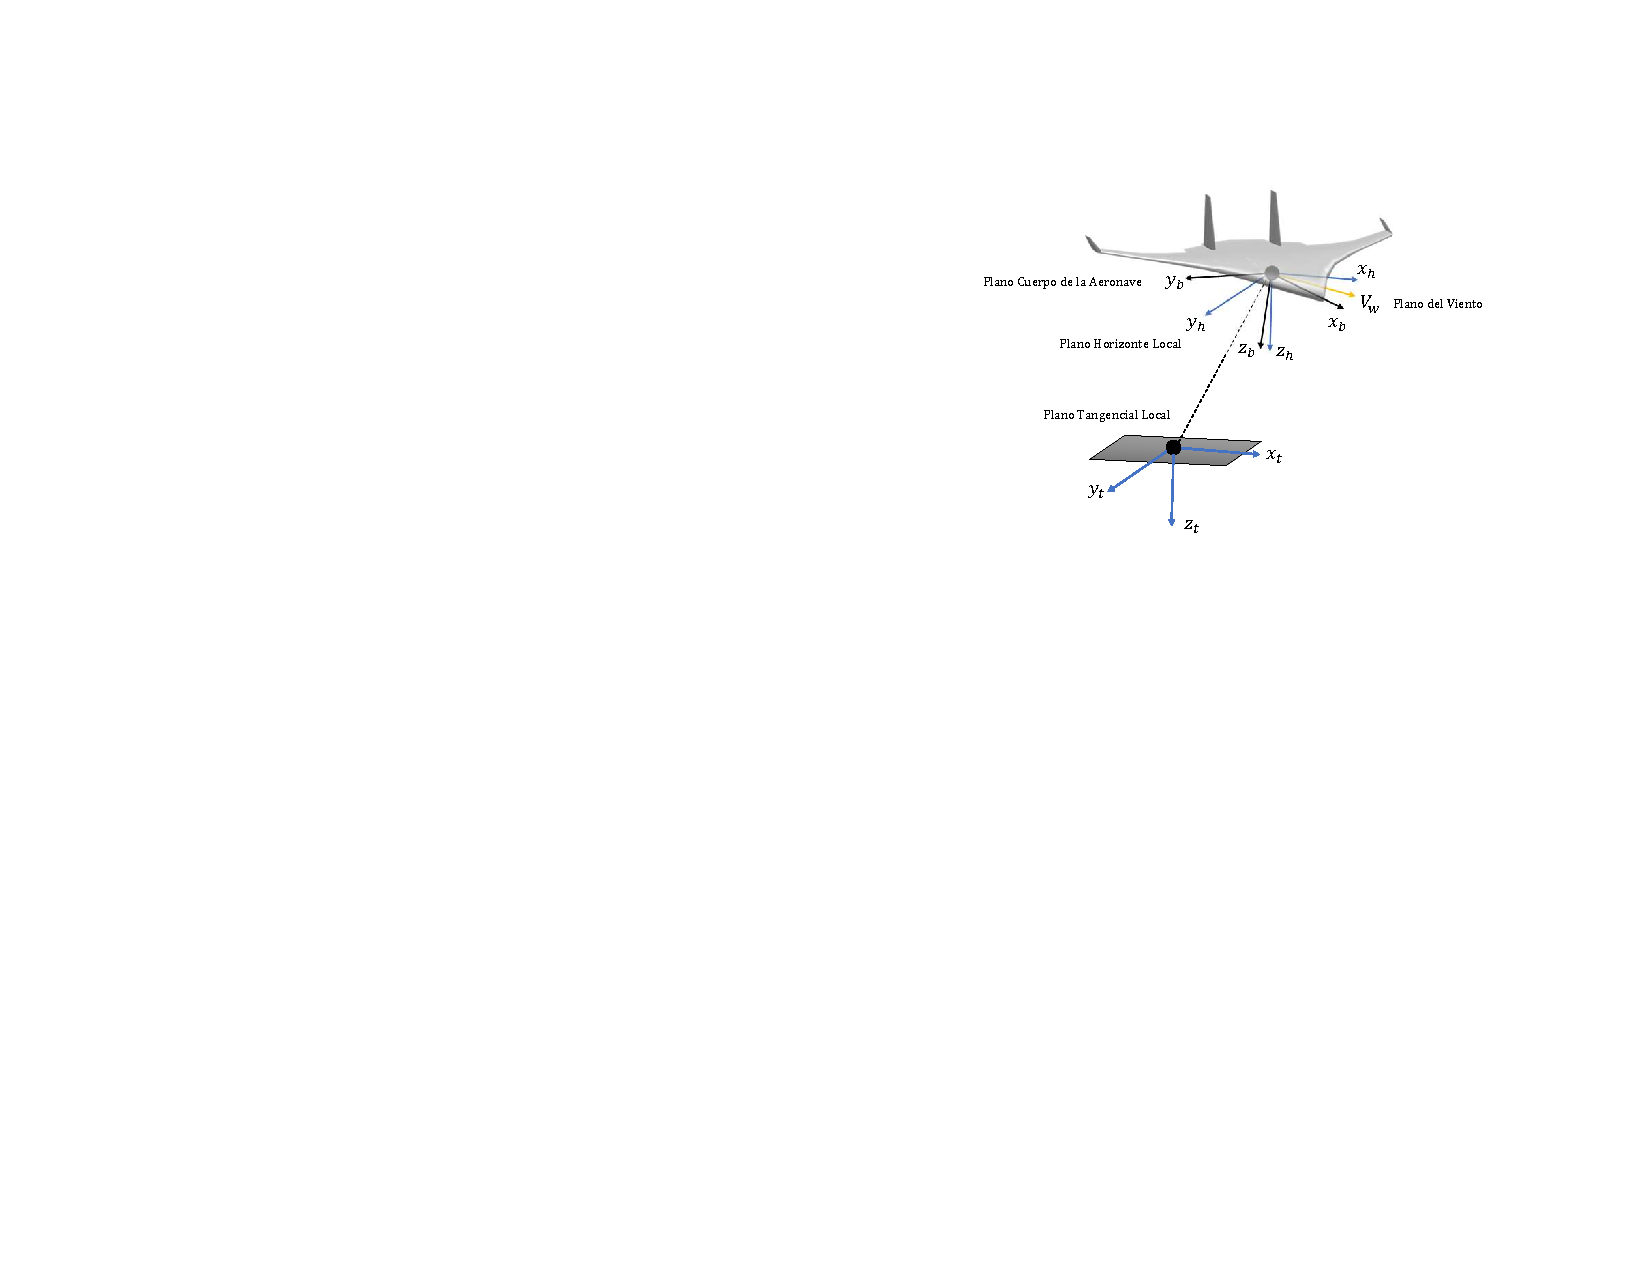
\includegraphics[scale=1.3]{Capitulo3/figs/Sistema de referencia Full_cropped (1).pdf}
\caption{EHEKATL BWB Reference System}
\label{Sistema de Referencia de EHEKATL BWB}
\end{figure}

The origin of the plane coordinates of the aircraft's local horizon and plane body are located in the centre of gravity of the aircraft.

The coordinates of the local horizon plane are permanently in the same orientation as the local tangential plane. The transformation of the local horizon plane from the local tangential plane defines the position after the aircraft's translation.  

The plane body coordinates of the aircraft are an orthogonal reference system fixed to the body of the aircraft, so we can measure the rotations of the axes of the plane body of the Aircraft with respect to the axes of the plane local horizon.

The aerodynamic forces and moments resulting from the aircraft-air interaction depend on the orientation of the aircraft body with the air speed vector. The magnitude of the air speed vector is opposite to the speed vector defined in LTP with respect to the ground speed, so this vector is the one that governs the aircraft's trajectory. 

%%%%%%%%%%%%%%%$%%%%
\section{Kinematics}
The kinematics studies the movement of a body according to its position and state regardless of the causes that originate it.

The transformation or relationship between the different reference systems is the central approach of kinematics to know the transfer and rotation movements of the aircraft. 
%
From the movements in the plane body of the aircraft with respect to the plane of horizontal horizon we can know the attitude of the aircraft in time, and multiplying the transformation matrix by the linear speeds of each axis we can obtain the \textbf{navigation matrix}. 
%
The implementation of the local tangent planes, local horizon, aircraft body and wind allow to determine the changes of position and orientation of EHEKATL BWB. 

\bigskip
%%%%%%%%%%%%%%%%%%%%%%%%%%%%%%%%%%%%%%%%%%%%%%%%%%%%%%%%%%%%%%%%%%%%%%%%%%%%%%%%%%%%%
\textbf{ Translational and Rotational Cinematics}\\
%%%%%%%%%%%%%%%%%%%%%%%%%%%%%%%%%%%%%%%%%%%%%%%%%%%%%%%%%%%%%%%%%%%%%%%%%%%%%%%%%%%
The coordinate systems considered in the \textbf{attitude of the angles of Euler} are based on the plane of the aircraft's local horizon and plane body. 
%
There are three degrees of freedom in rotational kinematics (heading, rolling and yawing) and three degrees of freedom in translational kinematics (axial, normal and lateral).
%
First, rotational kinematics is studied. Euler’s theorem states: “Any number of rotations with respect to different axes from a similar point, in the end, must be identified as a simple rotation.”\\
The transformation sequence is expressed below. 

\begin{figure}[h]
\centering
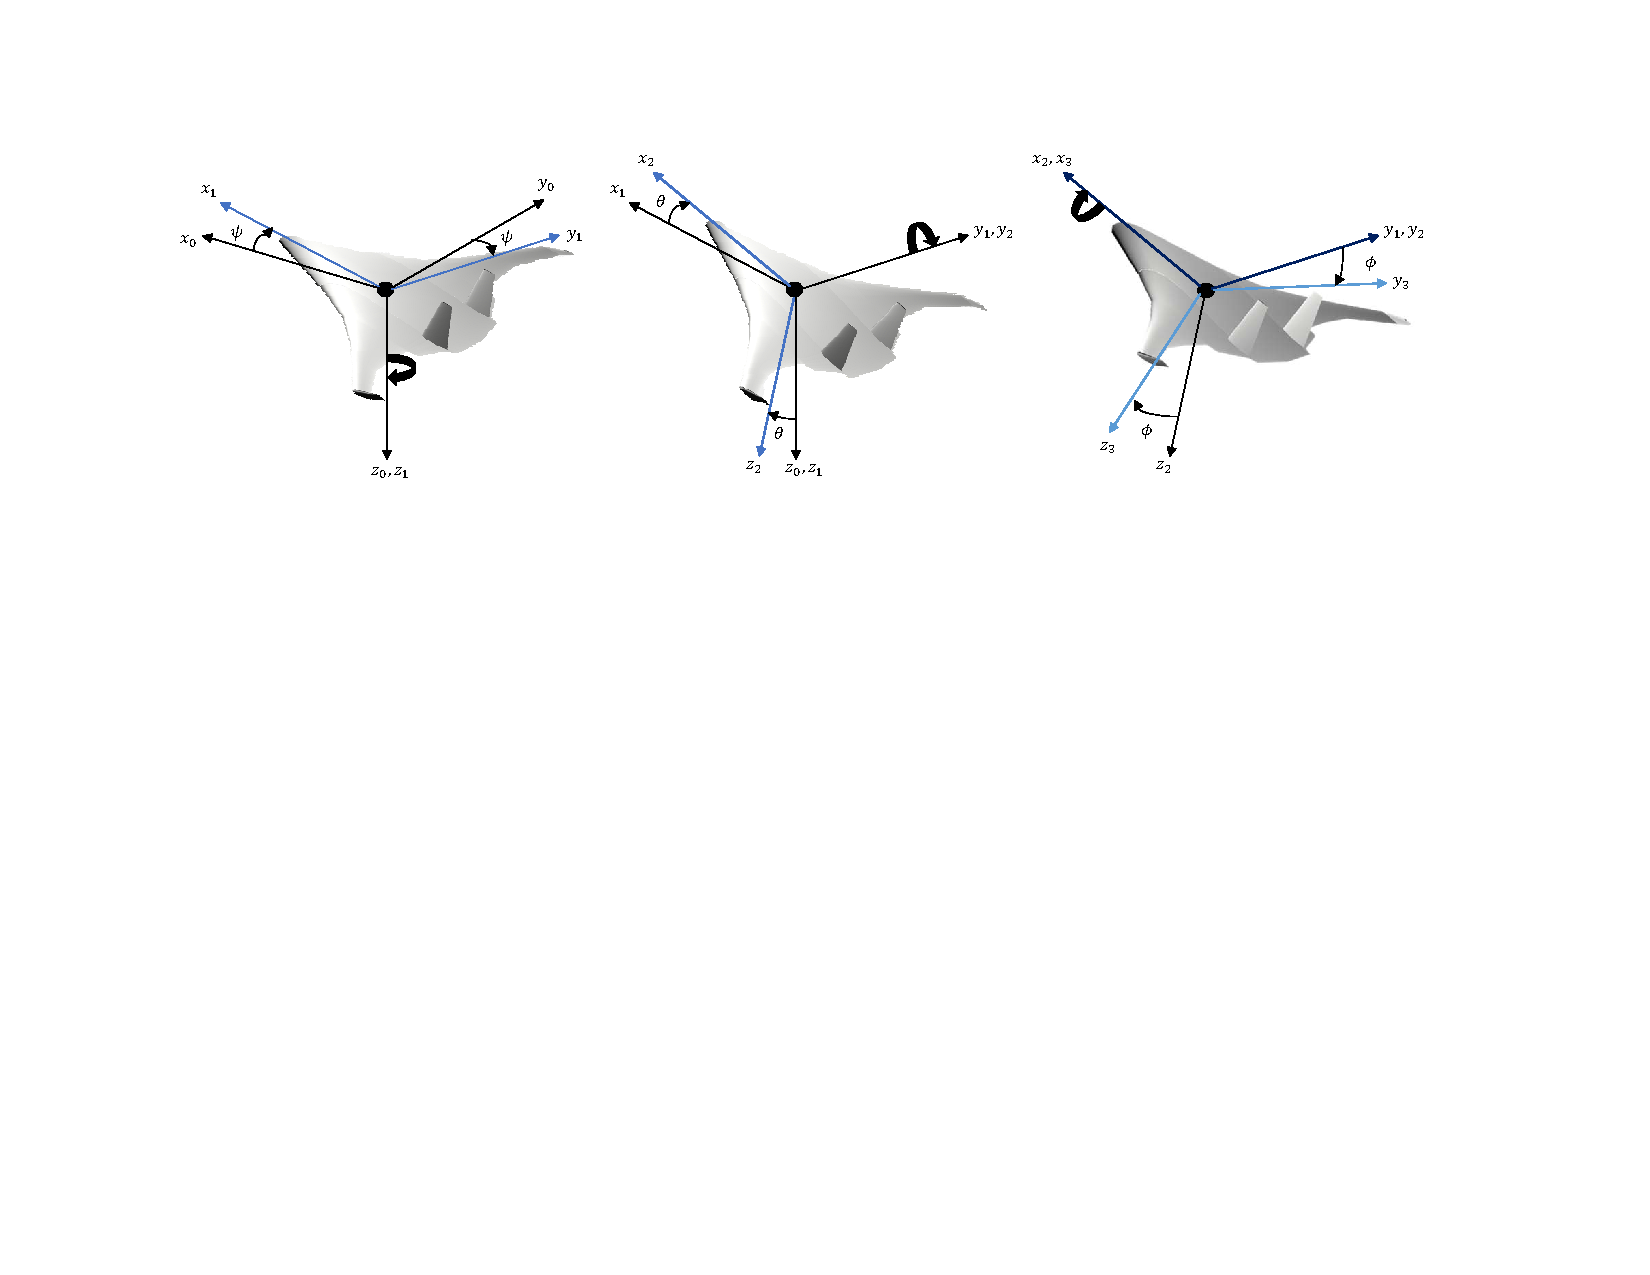
\includegraphics[scale=0.63]{Capitulo3/figs/cinematica ehekatl 1_cropped (1).pdf}
\caption{Rotation sequence: yaw, head and wing}
\label{fig: secuencia de rotación}
\end{figure}

\begin{equation}
    X_{0} \Rightarrow T_{\psi} \Rightarrow X_{1} \Rightarrow T_{\theta} \Rightarrow X_{2} \Rightarrow T_{\phi} \Rightarrow X_{3}
\end{equation}
All rotations are positive by following the right hand rule.

The transformation of the vector $X_{0} \Rightarrow T_{\psi} \Rightarrow X_{1}$ is expressed in matrix notation as:

\begin{gather}
    \begin{bmatrix}
    x_{1}\\
    y_{1}\\
    z_{1}
    \end{bmatrix}
    =
    \begin{bmatrix}
    C_{\psi} & S_{\psi} & 0\\
    -S_{\psi} & C_{\psi} & 0\\
    0 & 0 & 1
    \end{bmatrix}
    \begin{bmatrix}
    x_{0}\\
    y_{0}\\
    z_{0}
    \end{bmatrix}
\end{gather}

\begin{equation}
    X_{1} = T_{\psi}X_{0},\quad X_{0}= T^T_{\psi}X_{1}
\end{equation}

The transformation of the vector $X_{1} \Rightarrow T_{\theta} \Rightarrow X_{2}$ is expressed in matrix notation as:

\begin{gather}
    \begin{bmatrix}
    x_{2}\\
    y_{2}\\
    z_{2}
    \end{bmatrix}
    =
    \begin{bmatrix}
    C_{\theta} & 0 & -S_{\theta}\\
    0 & 1 & 0\\
    S_{\theta} & 0 & C_{\theta}
    \end{bmatrix}
    \begin{bmatrix}
    x_{1}\\
    y_{1}\\
    z_{1}
    \end{bmatrix}
\end{gather}

\begin{equation}
    X_{2} = T_{\theta}X_{1},\quad X_{1}= T^T_{\theta}X_{2}
\end{equation}

The transformation of the vector $X_{2} \Rightarrow T_{\phi} \Rightarrow X_{3}$ is expressed in matrix notation as:

\begin{gather}
    \begin{bmatrix}
    x_{3}\\
    y_{3}\\
    z_{3}
    \end{bmatrix}
    =
    \begin{bmatrix}
    1 & 0 & 0\\
    0 & C_{\phi} & S_{\phi}\\
    0 & -S_{\phi} & C_{\phi}
    \end{bmatrix}
    \begin{bmatrix}
    x_{2}\\
    y_{2}\\
    z_{2}
    \end{bmatrix}
\end{gather}

\begin{equation}
    X_{3} = T_{\phi}X_{2},\quad X_{2}= T^T_{\phi}X_{3}
\end{equation}

The final transformation of the plane body of the aircraft from the local horizon plane is the orderly multiplication of the individual transformation matrices shown as:

\begin{figure}[h]
\centering
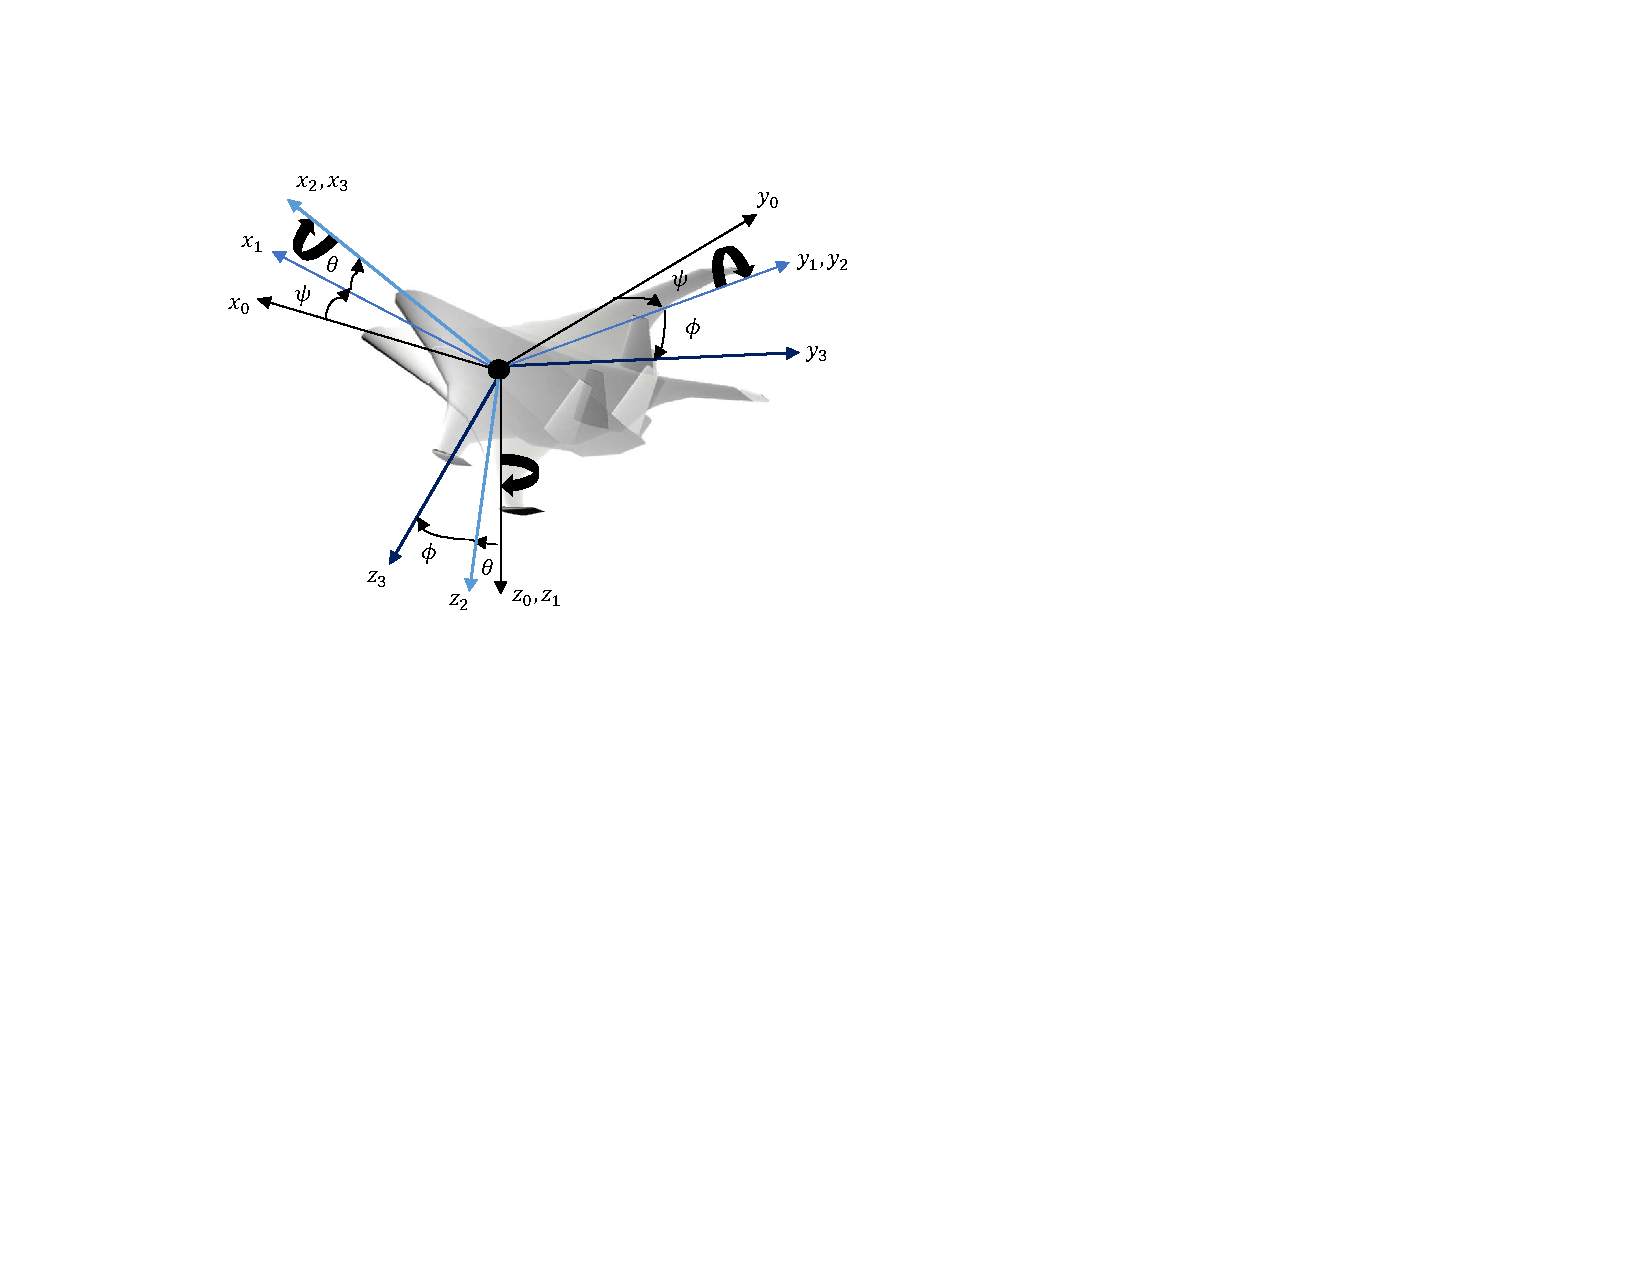
\includegraphics[scale=1]{Capitulo3/figs/cinematica ehekatl 2_cropped.pdf}
\caption{Rotation sequence of Euler angles}
\label{fig:x cubed graph}
\end{figure}


\begin{gather}
    \begin{bmatrix}
    x_{b}\\
    y_{b}\\
    z_{b}
    \end{bmatrix}
    =
    T_{\psi} T_{\theta} T_{\phi} 
    \begin{bmatrix}
    x_{n}\\
    y_{n}\\
    z_{n}
    \end{bmatrix}
\end{gather}

\begin{gather}
    \begin{bmatrix}
    x_{n}\\
    y_{n}\\
    z_{n}
    \end{bmatrix}
    =
    \begin{bmatrix}
    T_{\psi} & T_{\theta} & T_{\phi} 
    \end{bmatrix} ^T
    \begin{bmatrix}
    x_{b}\\
    y_{b}\\
    z_{b}
    \end{bmatrix}
\end{gather}

For simplification we will say that $S = T_{\psi} T_{\theta} T_{\phi}$where:
\begin{gather}
    S
    =
    \begin{bmatrix}
    C_{\psi} C_{\theta} & S_{\psi} C_{\theta} & -S_{\theta}\\
    C_{\psi} S_{\theta} S_{\phi} - S_{\psi} C_{\phi} & S_{\psi} S_{\theta} S_{\phi} + C_{\psi} C_{\phi} & C_{\theta} S_{\phi} \\
    C_{\psi} S_{\theta} C_{\phi} + S_{\psi} S_{\phi} & S_{\psi} S_{\theta} C_{\phi} - C_{\psi} S_{\phi} & C_{\theta} C_{\phi}
    \end{bmatrix}
\end{gather}

Whereas:
\begin{gather}
    S^T 
    =
    \begin{bmatrix}
    C_{\psi} C_{\theta} & C_{\psi} S_{\theta} S_{\phi} - S_{\psi} C_{\phi} & C_{\psi} S_{\theta} C_{\phi} + S_{\psi} S_{\phi}  \\
    S_{\psi} C_{\theta} &  S_{\psi} S_{\theta} S_{\phi} + C_{\psi} C_{\phi} & S_{\psi} S_{\theta} C_{\phi} - C_{\psi} S_{\phi} \\
    -S_{\theta} & C_{\theta} S_{\phi} & C_{\theta} C_{\phi} 
    \end{bmatrix}
\end{gather}

On the other hand, aircraft speed components $V_b = [u,v,w]^T$ are known in the body of the aircraft. Then the absolute speed components in the inertial reference system can be used according to the transformation relationships seen previously, knowing that $V_{b}$ is known, and we want to find $V_{inercial}$ o $V_{h}$, i.e.

\begin{gather}
\label{vh 1}
    \begin{bmatrix}
    \dot x_{h}\\
    \dot y_{h}\\
    \dot z_{h}
    \end{bmatrix}
    =
    S^T
    \begin{bmatrix}
    u\\
    v\\
    w
    \end{bmatrix}
\end{gather}

where

\begin{gather}
    V_{b}
    =
    \begin{bmatrix}
    u & v & w 
    \end{bmatrix}^T
\end{gather}

\begin{gather}
    V_{h}
    =
    \begin{bmatrix}
    \dot x_{h} & \dot y_{h} & \dot z_{h} 
    \end{bmatrix}^T
\end{gather}

Such that the equation \ref{vh 1} can be expressed as:
\begin{equation}
    V_{h} = S_{h/b}^{T} V_{b}
\end{equation}

o bien:
\begin{equation}
    V_{b} = S_{b/h} V_{h}
\end{equation}


\textbf{Nota:} The equation of $V_{b}$ can be integrated with respect to time by seeking to obtain the position in time of the aircraft's centre of gravity with respect to the inertial plane. This technique is suitable for use in simulators when you want to follow the aircraft's maneuver path. It is also necessary to know the history in time of the Euler angles as well as the speeds, in order to obtain a complete description for simulation purposes.

\medskip

Now consider the situation where an aircraft experiences an angular rotation given the velocity vector $\Omega$ with its components on the plane body of the aircraft.

\begin{gather}
    \Omega
    =
    \begin{bmatrix}
    p\\
    q\\
    r
    \end{bmatrix}
\end{gather}

The vector $\Omega$ can be described by the aligned components of Euler angle speeds $ \dot \phi, \dot \theta, \dot \psi$ defined by $\Delta \Omega_{\phi} + \Delta \Omega_{\theta} + \Delta \Omega_{\psi}$.

Then, each of the terms would be described as shown below.

\begin{gather}
\label{euler1}
    \Delta \Omega_{\phi}
    =
    T_{\phi}
    \begin{bmatrix}
    \dot \phi\\
    0\\
    0
    \end{bmatrix}
\end{gather}

\begin{gather}
    \Delta \Omega_{\theta}
    =
    T_{\phi} T_{\theta}
    \begin{bmatrix}
    0\\
    \dot \theta\\
    0
    \end{bmatrix}
\end{gather}

\begin{gather}
\label{eueler2}
    \Delta \Omega_{\psi}
    =
    T_{\phi} T_{\theta} T_{\psi}
    \begin{bmatrix}
    0\\
    0\\
    \dot \psi
    \end{bmatrix}
\end{gather}

Therefore we can define the vector of angular velocities of the body with respect to the Euler angle speeds as follows:

\begin{gather}
\label{velocidad angular aeronave}
    \begin{bmatrix}
    p\\
    q\\
    r
    \end{bmatrix}
    =
    \begin{bmatrix}
    1 & 0 & -S_{\theta}\\
    0 & C_{\phi} & C_{\theta} S_{\phi}\\
    0 & -S_{\phi} & C_{\theta} C_{\phi}
    \end{bmatrix}
    \begin{bmatrix}
    \dot \phi\\
    \dot \theta\\
    \dot \psi
    \end{bmatrix}
\end{gather}

In \ref{euler1}-\ref{eueler2} was used \textit{the theorem of the addition of angular speeds}. The theorem states that for an angular velocity vector coordinated in a reference system, the angular velocity vector resulting from the accumulated rotations is a simple sum of the contribution of each rotation. So, if the plane body of the aircraft is rotated given the set of Euler angles in variant time, defined with respect to the local horizon plane as stationary reference system, we can determine the components of the angular velocity vector $\Omega$ as the parameters of the rotating reference system.

The difference that we can observe with respect to the transformation of the equation of the navigation variables, is that the components of the derivatives of the Euler angles are not normal with each other, therefore, the transformation of the equation of the angular velocities $p,q,r$ cannot be solved as an orthogonal matrix. This prevents us from using the matrix of cosine directors and we have to follow the sequence shown in \ref{euler1}-\ref{eueler2}. Since the transformation matrix is not unique, the inverse exists. Thus, obtaining the inverse of the transformation matrix of  \ref{velocidad angular aeronave}. 
\begin{gather}
    \begin{bmatrix}
    \dot \phi\\
    \dot \theta\\
    \dot \psi
    \end{bmatrix}
    =
    \begin{bmatrix}
    1 & S_{\phi} tan\theta & C_{\phi} tan\theta\\
    0 & C_{\phi} & -S_{\phi}\\
    0 & S_{\phi} sec\theta & C_{\phi} sec\theta
    \end{bmatrix}
    \begin{bmatrix}
    p\\
    q\\
    r
    \end{bmatrix}
\label{eq cinem rot}
\end{gather}

One of the disadvantages of using Euler angles are the singularities defined in: 
\begin{gather}
    -\pi \leqslant \psi \leqslant \pi \\
    -\pi / 2 \leqslant \theta \leqslant \pi / 2 \\
    -\pi \leqslant \phi \leqslant \pi
\end{gather}

To solve this problem, the quaternions are used mainly in more elaborate flight missions. 

\medskip
%%%%%%%%%%%%%%%%%%%%%%%%%%%%%%%%%%%%%%%%%%%%%%%%%%%%%%%%%%%%%%%%%%%%%%%%%%%%%%%
\textbf{Speed Vector}\\
The orientation of the speed vector with respect to the aircraft body axles establishes two significant angles in the production of the aerodynamic forces and moments, named \textbf{angle of attack $\alpha$} and \textbf{sliding or drifting angle $\beta$},  \cite{Schimdt1998}.
\begin{figure}[h]
\centering
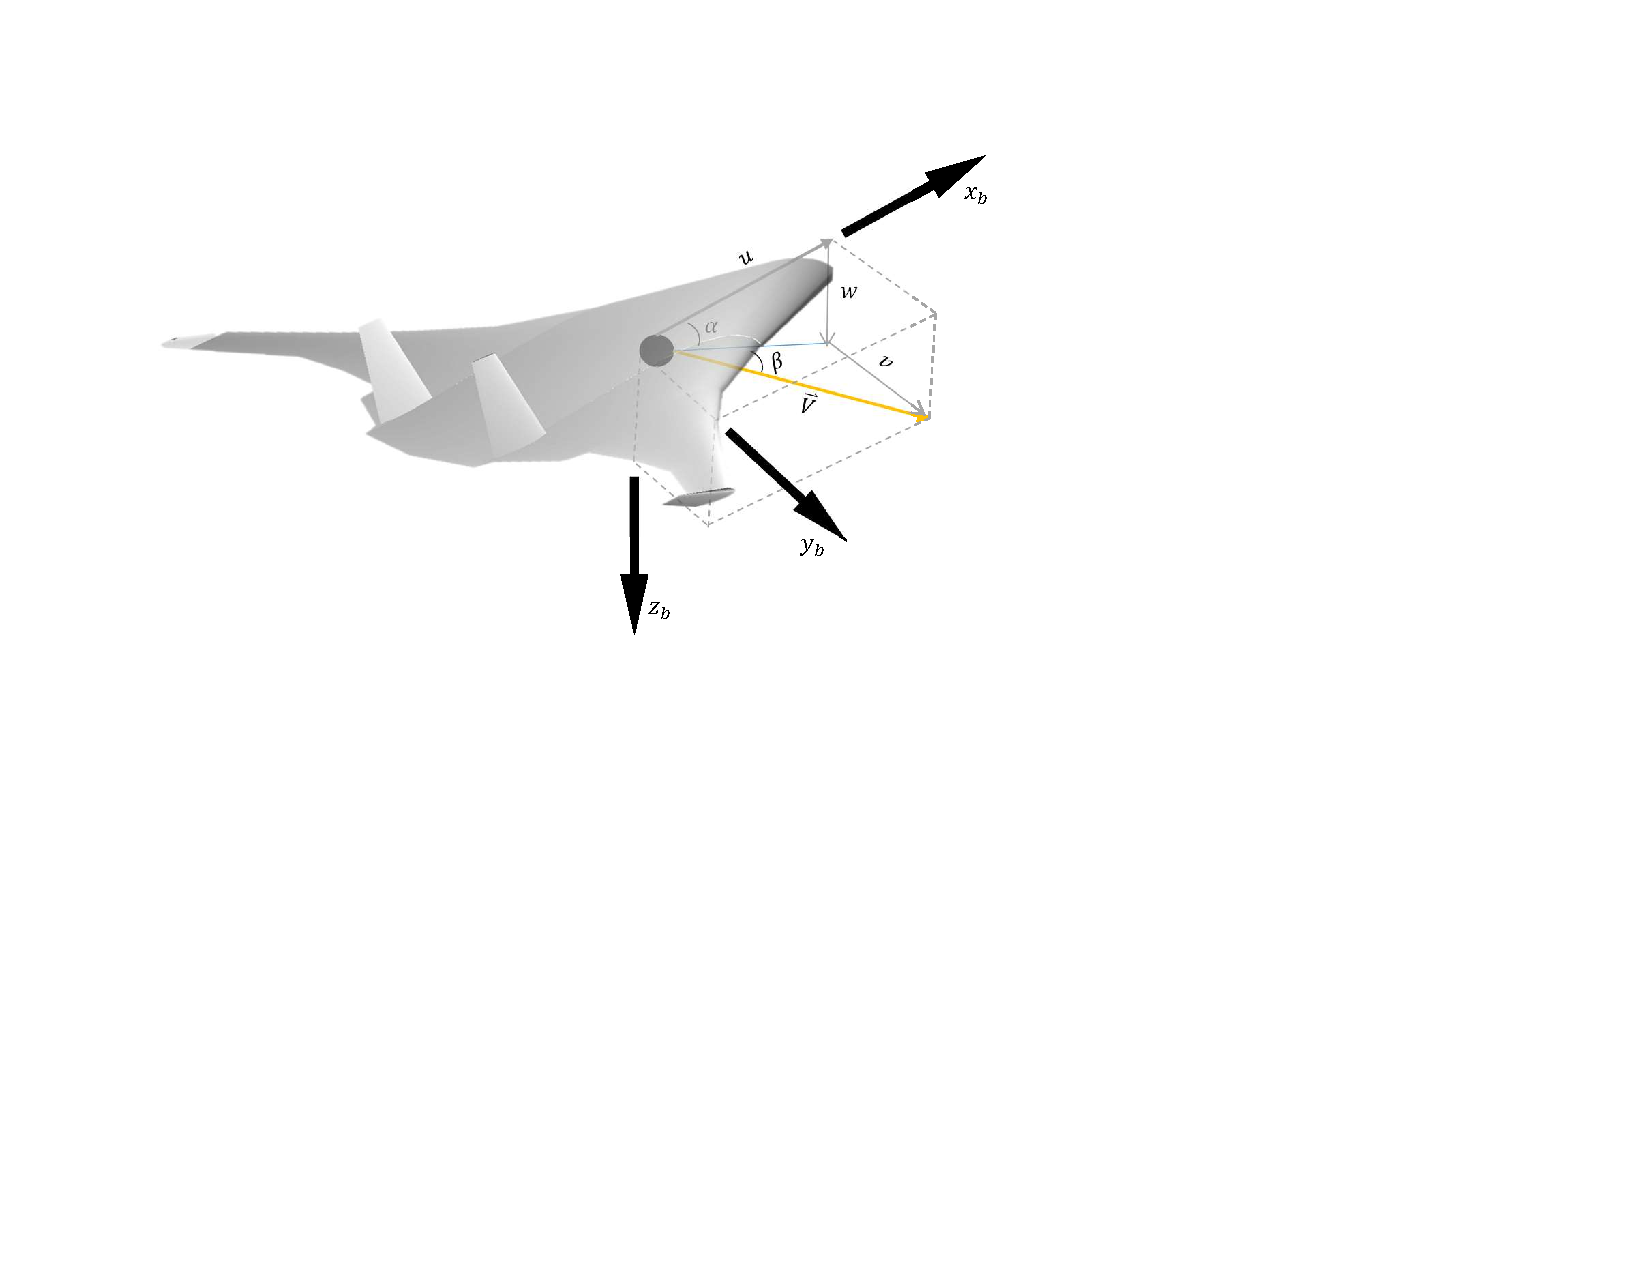
\includegraphics[scale=0.9]{Capitulo3/figs/angulo aerodinamico_cropped.pdf}
\caption{Aerodynamic angles}
\label{fig: angulos aerodinamicos}
\end{figure}

Linear speed components in the aircraft body $u$,$v$,$w$ are defined as

\begin{align}
\label{eq cossin V}
u &= V C_{\beta} C_{\alpha}\\
v &= V S_{\beta}\\
w &= V C_{\beta} S_{\alpha}
\end{align}

where:
\begin{equation}
    V = \sqrt{u^2 + v^2 + w^2}
\end{equation}

The angle of attack $\alpha$ can be obtained by the tangent function with respect to the components on the stability axis, $u$ and $w$, dando: $tan{(\alpha)}=u/w$. The angle of sliding or skidding $\beta$, is independent of the direction of plane of symmetry, and is obtained by the lateral component $v$ which is the opposite catet and our hypotenuse or result $\Vec{V}$, obteniendo: $sin{\beta}=v/V$.

The aerodynamic angles of the speed vector are defined:

\begin{equation}
\label{eq: angulos aero1}
  \alpha = tan^{-1} \frac{w}{u}  
\end{equation}

\begin{equation}
\label{eq: angulos aero2}
  \beta = sin^{-1} \frac{v}{V}
\end{equation}

\medskip

For small angles we assume the initial velocity as constant, $u_0 = V$, such that the variation of angles is small (considering the theory of small disturbances) \ref{eq: angulos aero1},\ref{eq: angulos aero2} are re-written as: 

\begin{align}
\label{eq: ángulos aerodinámicos con pequeñas perturbaciones}
\alpha &= \frac{w}{u}\\
\beta &= \frac{v}{V}
\end{align}

\medskip
%%%%%%%%%%%%%%%%%%%%%%%%%%%%%%%%%%%%%%%%%%%%%
\textbf{Uprising and Drag Forces}\\
The transformation of the stability axis from the aircraft body axis into the plane of plane symmetry is shown below. $x-z$ using the force vector represented by the sum of the components of the aerodynamic drag forces $D$ and Lifting $L$. The resulting force vector will then be rewritten as the force components $X$ and $Z$ on the body axles of the aircraft.  

It is assumed that the aircraft is in balanced flight (altitude and constant speed), implying that the speed vector is horizontal. 

\begin{figure}[h]
\centering
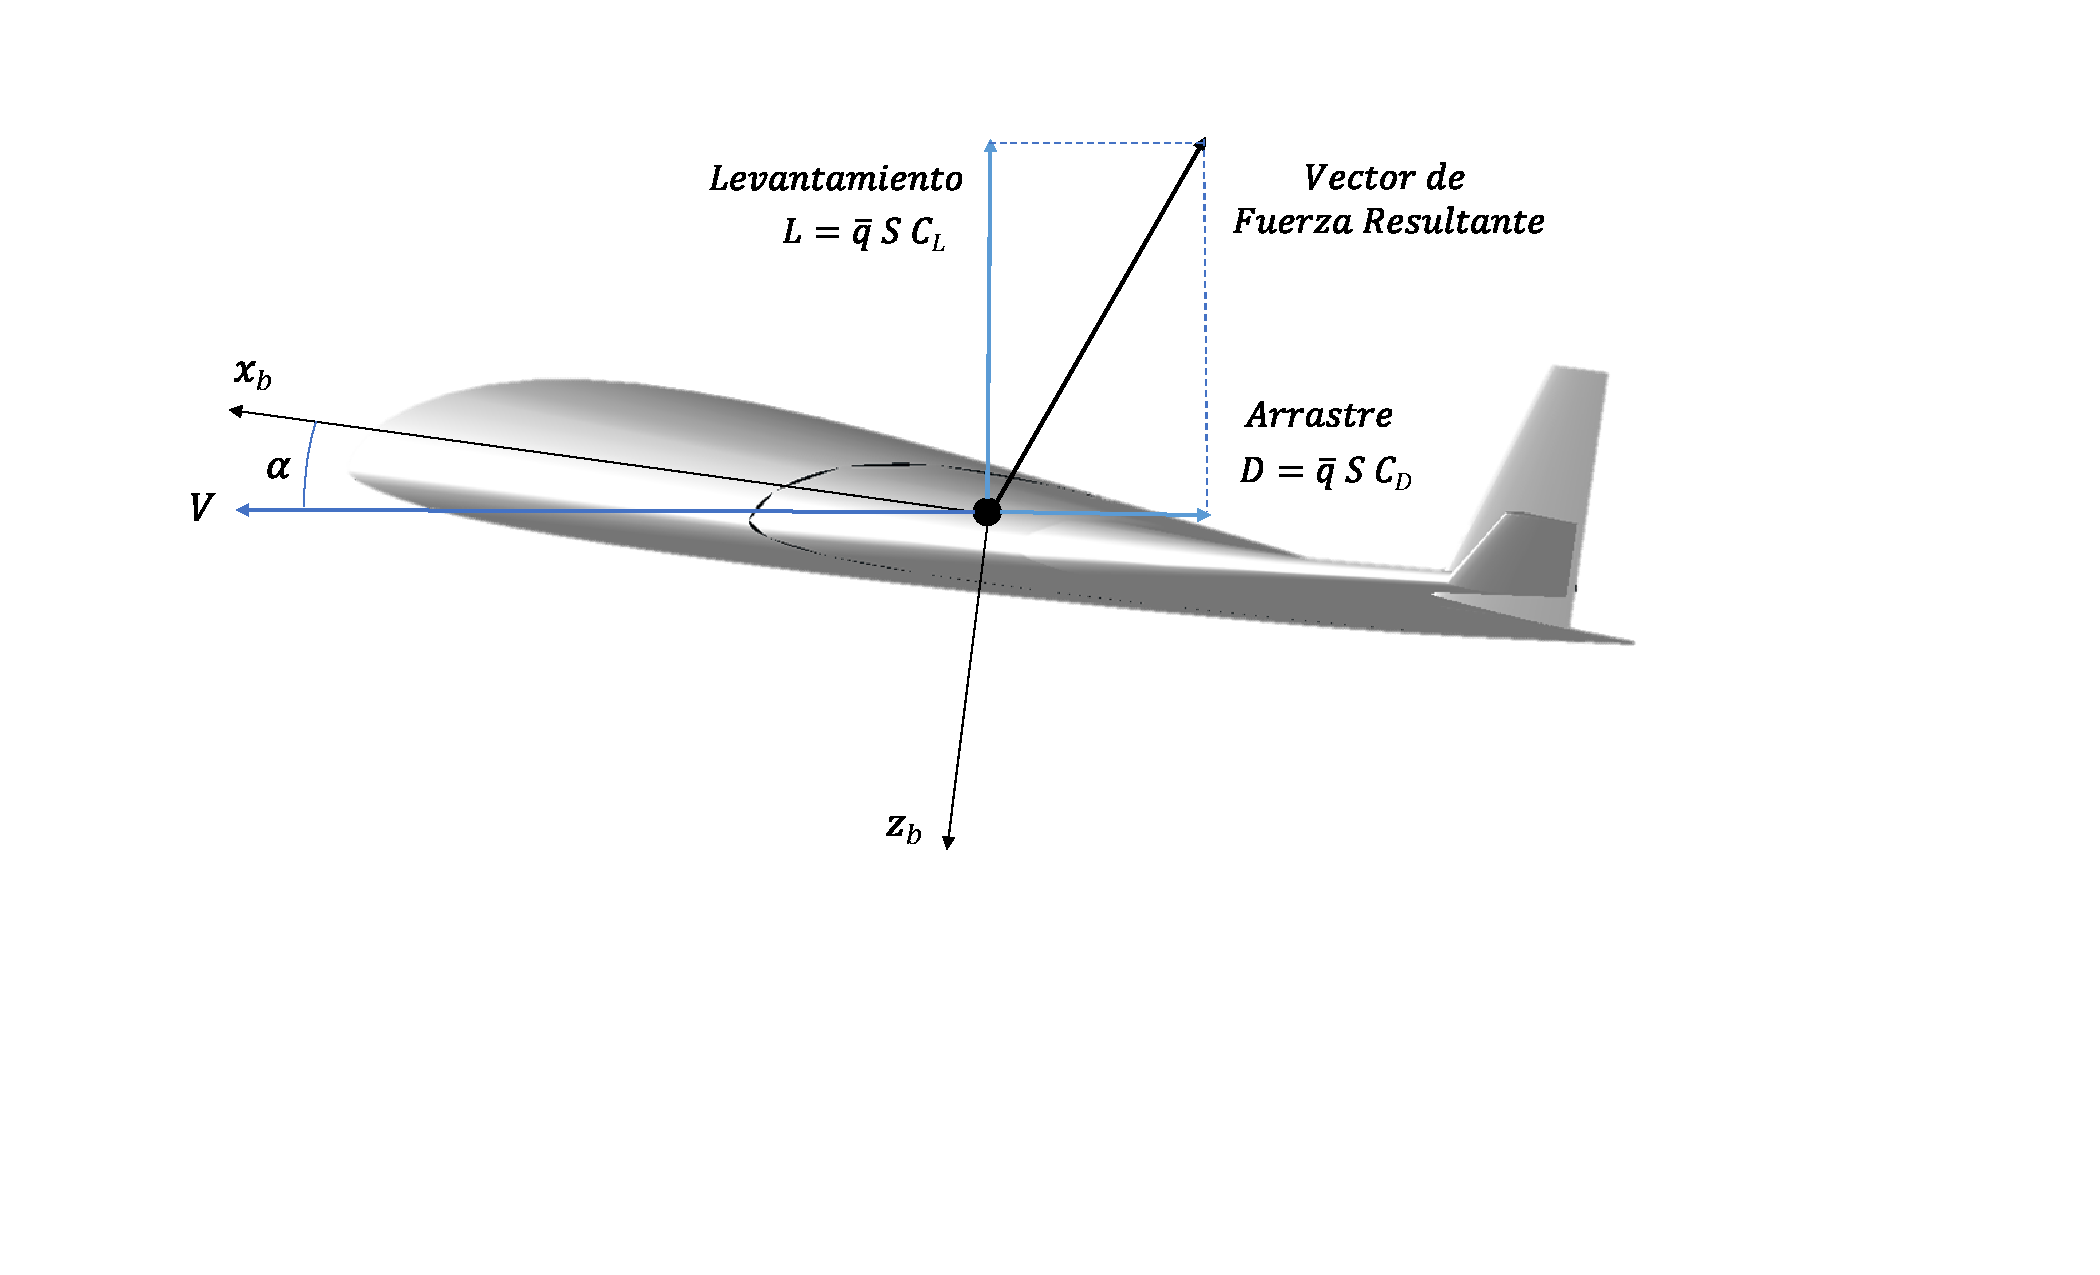
\includegraphics[scale=0.47]{Capitulo3/figs/fuerzas aerodinamicas_cropped.pdf}
\caption{Airplane force components during balancing flight}
\label{fig: fuerzas aerodinamicas}
\end{figure}

The forces $X,Z$ are oriented when generated at the angle of attack with respect to the reference plane at flight level or symmetry plane $x-z$. The lifting and dragging forces are combined into a resulting force, which can be considered as a vector described by the components of such a coordinate system, i.e. the components of the forces X and Z can be expressed in terms of L and D by the following equations: 

\begin{align}\
X = -D C_{\alpha}+LS_{\alpha}\\
Z = -D S_{\alpha} - LC_{\alpha}
\end{align}


In matrix notation:


\begin{gather} 
\begin{bmatrix}
X\\
Z
\end{bmatrix}
=
\begin{bmatrix}
-C_{\alpha} & S_{\alpha}\\ 
-S_{\alpha} & -C_{\alpha}
\end{bmatrix}
\begin{bmatrix}
 D\\
L
\end{bmatrix}
=
T_{\alpha}
\begin{bmatrix}
D \\
L
\end{bmatrix}
\end{gather}

where $T_{\alpha}$ represents the rotational angular transformation matrix of $\alpha$.

\medskip

Let us now consider the reverse direction by resolving the transformation of the coordinates of the aerodynamic forces with respect to the aircraft's body axes. 


\begin{gather} 
\begin{bmatrix}
D\\
L
\end{bmatrix}
=
\begin{bmatrix}
-C_{\alpha} & -S_{\alpha}\\ 
S_{\alpha} & -C_{\alpha}
\end{bmatrix}
\begin{bmatrix}
X\\
Z
\end{bmatrix}
=
T_{\alpha}^{-1}
\begin{bmatrix}
X \\
Z
\end{bmatrix}
\end{gather}

So, one can notice that the inverse matrix is equal to the transpose of the original matrix. $T_{\alpha}^{-1}=T_{\alpha}^T$, and by definition: is an orthogonal matrix; since its transposition is equal to its inverse.
%
When the angle is generated $\alpha$, podemos expresar $X,Z$ from the coordinate system  $L,D$. 

\medskip

%%%%%%%%%%%%%%%%%%
\section{Dynamics}
Dynamics studies the causes that originate the movement of the bodies. In this section the six equations of motion (six degrees of freedom) of the aircraft are developed considering the linear and angular forces that generate the movement.

 Newton's second law states that the sum of external forces acting on a body in an inertial reference system is equal to the rate of change in time according to its angular and linear moment. 

 The equations of aircraft flight mechanics based on the conservation of angular and linear momentum, are developed based mainly on the developments mentioned in \cite{Schimdt1998} and \cite{USAF1988}.

 \begin{figure}[!h]
\centering
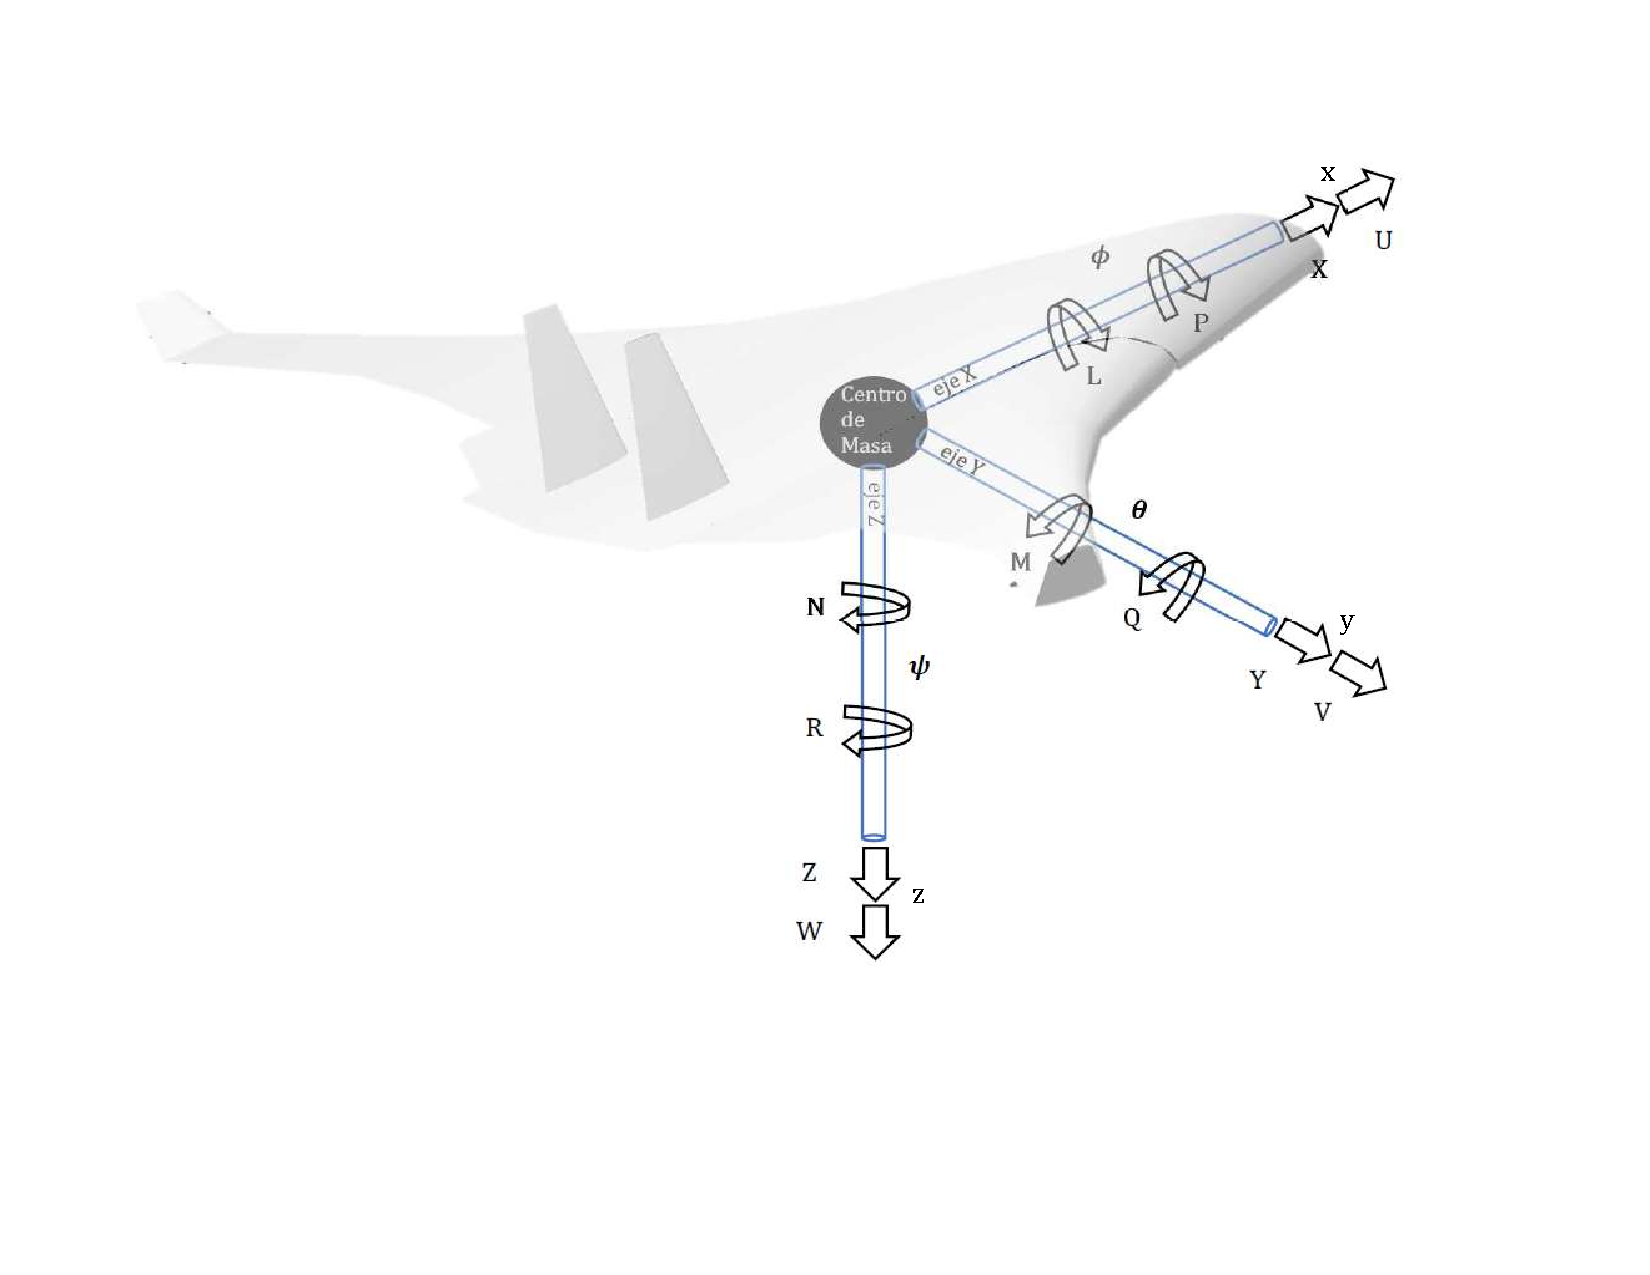
\includegraphics[scale=0.57]{Capitulo3/figs/dinamica ehekatl_cropped.pdf}
\caption{Position, speed, forces and moments applied to body axes}
\label{fig: posicion, velocidad, fuerzas y momentos}
\end{figure}
%
\begin{table}[!h]
\caption{Dynamic variables on aircraft body axles}
\centering
\begin{tabular}{|r|r|r|r|}
     \hline
    \textbf{Aircraft dynamics} & eje x & y-axis & eje z \\
     \hline
     Momento angular & L & M & N \\
     \hline
     Velocidad angular & p & q & r \\
     \hline
     Angular position & $\phi$ & $\theta$ & $\psi$ \\
     \hline
     Fuerza lineal & X & And & Z \\
     \hline
     Velocidad lineal & u & v & w \\
     \hline
     Linear position & x & and & z \\
     \hline
\end{tabular}
\label{tab: variables dinamicas}
\end{table}
 
In the Figure \ref{fig: posicion, velocidad, fuerzas y momentos} We have the general representation of the forces and moments that act as a component on each body axis of the aircraft (axis x, axis y, axis z). We have 6 degrees of freedom, a degree of linear and angular freedom for each axis.  

In the table \ref{tab: variables dinamicas} the variables considered in the Figure are defined \ref{fig: posicion, velocidad, fuerzas y momentos}.

\medskip

\textbf{Momento Lineal Traslacional}\\
Newton's second law defines translational movement as
\begin{equation}
\bar{F} = \frac{d}{dt}(m \bar{V})
\end{equation}
where $\bar{F}$ is the sum of the applied external linear forces and $m \bar{V}$ It's the linear moment.
$\bar{F}$ is a vector that can be represented in translational equations of 3 degrees of freedom (according to each component of the three-dimensional space).

The external force vector is defined as the sum of all forces applied to the aircraft $\bar{F}=F_{Aero}+F_{Gravedad}+F_{Propulsion}+F_{Control}+F_{Perturbaciones}$. The above terms are developed in the following section: \textit{forces and moments applied}.

\begin{table}[!h]
\caption{Force and time applied to the aircraft}
\centering
\begin{tabular}{|r|r|r|r|r|r|}
     \hline
     $\bar{F}/\bar{G}$ & Aerodynamics & Gravedad & Propulsion & Control & Perturbaciones \\
     \hline
     \textbf{X} & $X_{A}$ & $X_{G}$ & $X_{T}$ & $X_{C}$ & $X_{P}$ \\
     \hline
     \textbf{And} & $Y_{A}$ & $Y_{G}$ & $Y_{T}$ & $Y_{C}$ & $Y_{P}$ \\
     \hline
     \textbf{Z} & $Z_{A}$ & $Y_{G}$ & $Y_{T}$ & $Z_{C}$ & $Z_{P}$ \\
     \hline
     \textbf{L} & $L_{A}$ & 0 & 0 & $L_{C}$ & $L_{P}$ \\
     \hline
     \textbf{M} & $M_{A}$ & 0 & 0 & $M_{C}$ & $M_{P}$ \\
     \hline
      \textbf{N} & $N_{A}$ & 0 & 0 & $N_{C}$ & $N_{P}$ \\
     \hline
\end{tabular}
\end{table}

The speed in the fixed inertial reference system of ground axles with respect to the aircraft body axle reference system is represented as

\begin{equation}
\label{momento lineal traslacional}
    F = m ( \frac{d \bar{V}}{dt}\mid_{x_{T} y_{T} z_{T}}) = m (\frac{d \bar{V}}{dt}\mid_{x_{B} y_{B} z_{B}} + \bar{\omega} \times \bar{V} )
\end{equation}

where a mass is assumed $m$ constante. $\bar{V}$ and $\bar{\omega}$ are the vectors for linear velocities $u,v,w$ and angular $p,q,r$, respectively.

\begin{equation}
    \bar{V} = u\bar{i}+v\bar{j}+w\bar{k} 
\end{equation}

\begin{equation}
    \bar{\omega} = p\bar{i}+q\bar{j}+r\bar{k} 
\end{equation}


In flight dynamics we have four vectors for aircraft motion equations ($\bar{V}, \bar{\omega}, \bar{F}, \bar{G}$), where $\bar{F}$ and $\bar{G}$ are the applied external forces and moments that we will develop later. 

\medskip

Developing the equation (\ref{momento lineal traslacional}) in its components we obtain

\begin{equation}
    \bar{F} = m(\dot{u}\bar{i}+\dot{v}\bar{j}+\dot{w}\bar{k}+\begin{bmatrix}
    \bar{i} & \bar{j} & \bar{k} \\
    p & q & r \\
    u & v & w
    \end{bmatrix}) 
\end{equation}


\begin{equation}
    \bar{F} = m(\dot{u}\bar{i}+\dot{v}\bar{j}+\dot{w}\bar{k}+
    (qw-rv)\bar{i} + (pw-ru)\bar{j} + (pv-qu)\bar{k}) 
\end{equation}

\begin{equation}
    \bar{F} = m((\dot{u}+qw-rv)\bar{i} + (\dot{v}+pw-ru)\bar{j} + (\dot{w}+pv-qu)\bar{k}) 
\end{equation}

Finally, the equations of the linear translational moment in its three-dimensional components are defined.

\begin{gather}
\label{eq: momento lineal}
    \bar{F} = F_x \bar{i} + F_y \bar{j} + F_z \bar{k} = X + Y + Z 
\end{gather}

where

\begin{gather}
\label{eq dinam tras 1}
    X = m(\dot{u} + qw - rv) \\
    Y = m(\dot{v} + ru - pw) \\
    Z = m(\dot{w} + pv - qu)
\label{eq dinam tras 2}
\end{gather}


\medskip
%%%%%%%%%%%%%%%%%%%%%%%%%%%%%%%%%%%%%%%%%%%%%%%%%%%%%%%%%%%%%%%%%%%%%%%%%%%%%
\textbf{Momento Angular Rotacional}\\
In the same way as the vector of external forces $\bar{F}$ changes the linear moment ($\bar{F}=\frac{d}{dt}m\bar{V}$), external moments $\bar{G}$ change angular momentum ($\bar{G}=\frac{d}{dt}\bar{H}$).

Newton's second law defines rotational movement

\begin{equation}
\label{eq: movimiento rotacional}
\bar{G} = \frac{d}{dt}(\bar{H})
\end{equation}

where $\bar{G}$ is the sum of the external moments applied $\bar{G}=G_{Aero}+G_{Propulsion}+G_{Control}+G_{Perturbaciones}$ and $\bar{H}$ is the angular moment applied. 
$\bar{G}$ is a vector that can be represented in three rotational equations of 3 degrees of freedom (according to each component of the three-dimensional space). We can understand the angular moment as a linear moment with lever arm included. 

\begin{gather}
    \bar{P} = m\bar{V} \\
    \bar{H} = \bar{r} \times \bar{P}
\end{gather}

where $\bar{P}$ is the linear moment and  $\bar{r}$ It's the lever arm, the angle between $\bar{r}$ and $\bar{V}$ is 90° and the magnitude of the angular moment is $mrV$. 

Defining the products and moments of inertia, the angular momentum equation of a rigid body is established 

\begin{equation}
    \bar{H} = H_x \bar{i} + H_y \bar{j} + H_z \bar{k}
\end{equation}

Entonces

\begin{gather}
    H_x = p I_{x} - q I_{xy} - r I_{xz} \\
    H_y = q I_{y} - r I_{yz} - p I_{xy} \\
    H_z = r I_{z} - p I_{xz} - q I_{yz}
\end{gather}

%% Define the equations of an airplane which is completely asymmetric
%% Then explain what the plane of symmetry is, and reduce the equations

Considering that the x-z body axes are in the plane of symmetry of the aircraft, we can reduce two inertia products, such that $I_{xy} = I_{yz} = 0$. With this consideration the angular momentum equation of a symmetric aircraft is simplified

\begin{equation}
    \bar{H} = (p I_{x} - r I_{xz})\bar{i} + q I_{y}\bar{j} + (r I_{z} - p I_{xz})\bar{k} 
\end{equation}

And remembering the equation (\ref{eq: movimiento rotacional}) we can express it according to the inertial system of the terrestrial axes. 

\begin{equation}
    \bar{G} = \frac{d\bar{H}}{dt} | x_T y_T z_T
\end{equation}

Expressing on the body axles of the aircraft 

\begin{equation}
    \bar{G} = \frac{d\bar{H}}{dt} | x_B y_B z_B + \bar{\omega} \times \bar{H}
\end{equation}

Developing, we have to

\begin{equation}
    \bar{G} = \dot{H}_{x} \bar{i} + \dot{H}_{y} \bar{j} + \dot{H}_{z} \bar{k} + \begin{bmatrix}
    \bar{i} & \bar{j} & \bar{k} \\
    p & q & r \\
    H_{x} & H_{y} & H_{z}
    \end{bmatrix}
\end{equation}

Since the body of the aircraft is assumed to be a rigid body, the moments and products of inertia are constant. 

\begin{equation}
    \bar{G} = (\dot{p} I_{x} - \dot{r} I_{xz})\bar{i} + \dot{q} I_{y}\bar{j} + (\dot{r} I_{z} - \dot{p} I_{xz})\bar{k} + \begin{bmatrix}
    \bar{i} & \bar{j} & \bar{k} \\
    p & q & r \\
    (p I_{x} - r I_{xz}) & q I_{y} & (r I_{z} - p I_{xz})
    \end{bmatrix} 
\end{equation}

Therefore, the three-dimensional rotational components are

\begin{gather}
\label{eq: momento angular 1}
    G_x = \dot{p} I_{x} + qr (I_{z} - I_{y}) - (\dot{r} + pq) I_{xz} \\
    G_y = \dot{q} I_{y} - pr (I_{z} - I_{x}) + (p^2 - r^2) I_{xz} \\
    G_z = \dot{r} I_{z} + pq (I_{y} - I_{x}) + (qr - \dot{p}) I_{xz}
\label{eq: momento angular 2}
\end{gather}

And with this we have complete the set of rotational equations. In the next section the applied forces and moments are developed, $\bar{F}$ and $\bar{G}$. 

\bigskip
%%%%%%%%%%%%%%%%%%%%%%%%%%%%%%%%%%%%%%%%%%%%%%%%%%%%%%%%%%%%%%%%%%%%%%
\section{Applied Forces and Moments}

The forces and moments applied to the aircraft are equal to the sum of the terms of the forces: aerodynamics $_A$, of gravity  $_G$, propulsion  $_T$, Control  $_C$ and atmospheric disturbances $_P$. According to linear conservation equations \ref{eq dinam tras 1}-\ref{eq dinam tras 2} and angular conservation \ref{eq: momento angular 1}-\ref{eq: momento angular 1} can be defined



\begin{align}
    X_{A} + X_{G} + X_{T} + X_{C} + X_{P} &= m (\dot u + qw - rv) \\
    Y_{A} + Y_{G} + Y_{T} + Y_{C} + Y_{P} &= m (\dot v + ru - pw) \\
    Z_{A} + Z_{G} + Z_{T} + Z_{C} + Z_{P} &= m (\dot w + pv - qu) \\
    L_{A} + L_{T} + L_{C} + L_{P} &= \dot p I_{x} + qr(I_{z} - I_{y}) - (\dot r + pq)I_{xz} \\
    M_{A} + M_{T} + M_{C} + M_{P}  &= \dot q I_{y} + pr(I_{z} - I_{x}) + (p^2 - r^2)I_{xz} \\
    N_{A} + N_{T} + N_{C} + N_{P} &= \dot r I_{z} + pq(I_{y} - I_{z}) + (qr - \dot p)I_{xz}
\end{align}


%%%%%%%%%%%%%%%%%%%%%%%%%%%%%%%%%%%%%%%%%%%%%%%%%%%%%%%%%%%%%%%%%%%%%%%%%%%%%%%%%%%%%%%%%%%%
\textbf{Force of Gravity}


Assuming that the altitude of the aircraft is not significant compared to the radius of the ground, it is sufficient to consider the magnitude of gravity as constant. 

The weight of the aircraft (gravity force) will enter into the equations of motion represented in a component by each body axis of the aircraft. We consider the weight of the aircraft $W=mg$ in the inertial reference plane (local horizon plane) since the gravitational force is assumed as a linear and constant force towards the center of the earth. \ref{fig: fuerza gravitacional} we can observe the transformation of the body of the aircraft, where in its initial condition, the axis $x_b$ is parallel and matching to the axis $x_h$, and after a nodding motion, the axis $x_b$ has a certain angular distance from the axis $x_h$.  
\begin{figure}[!h]
\centering
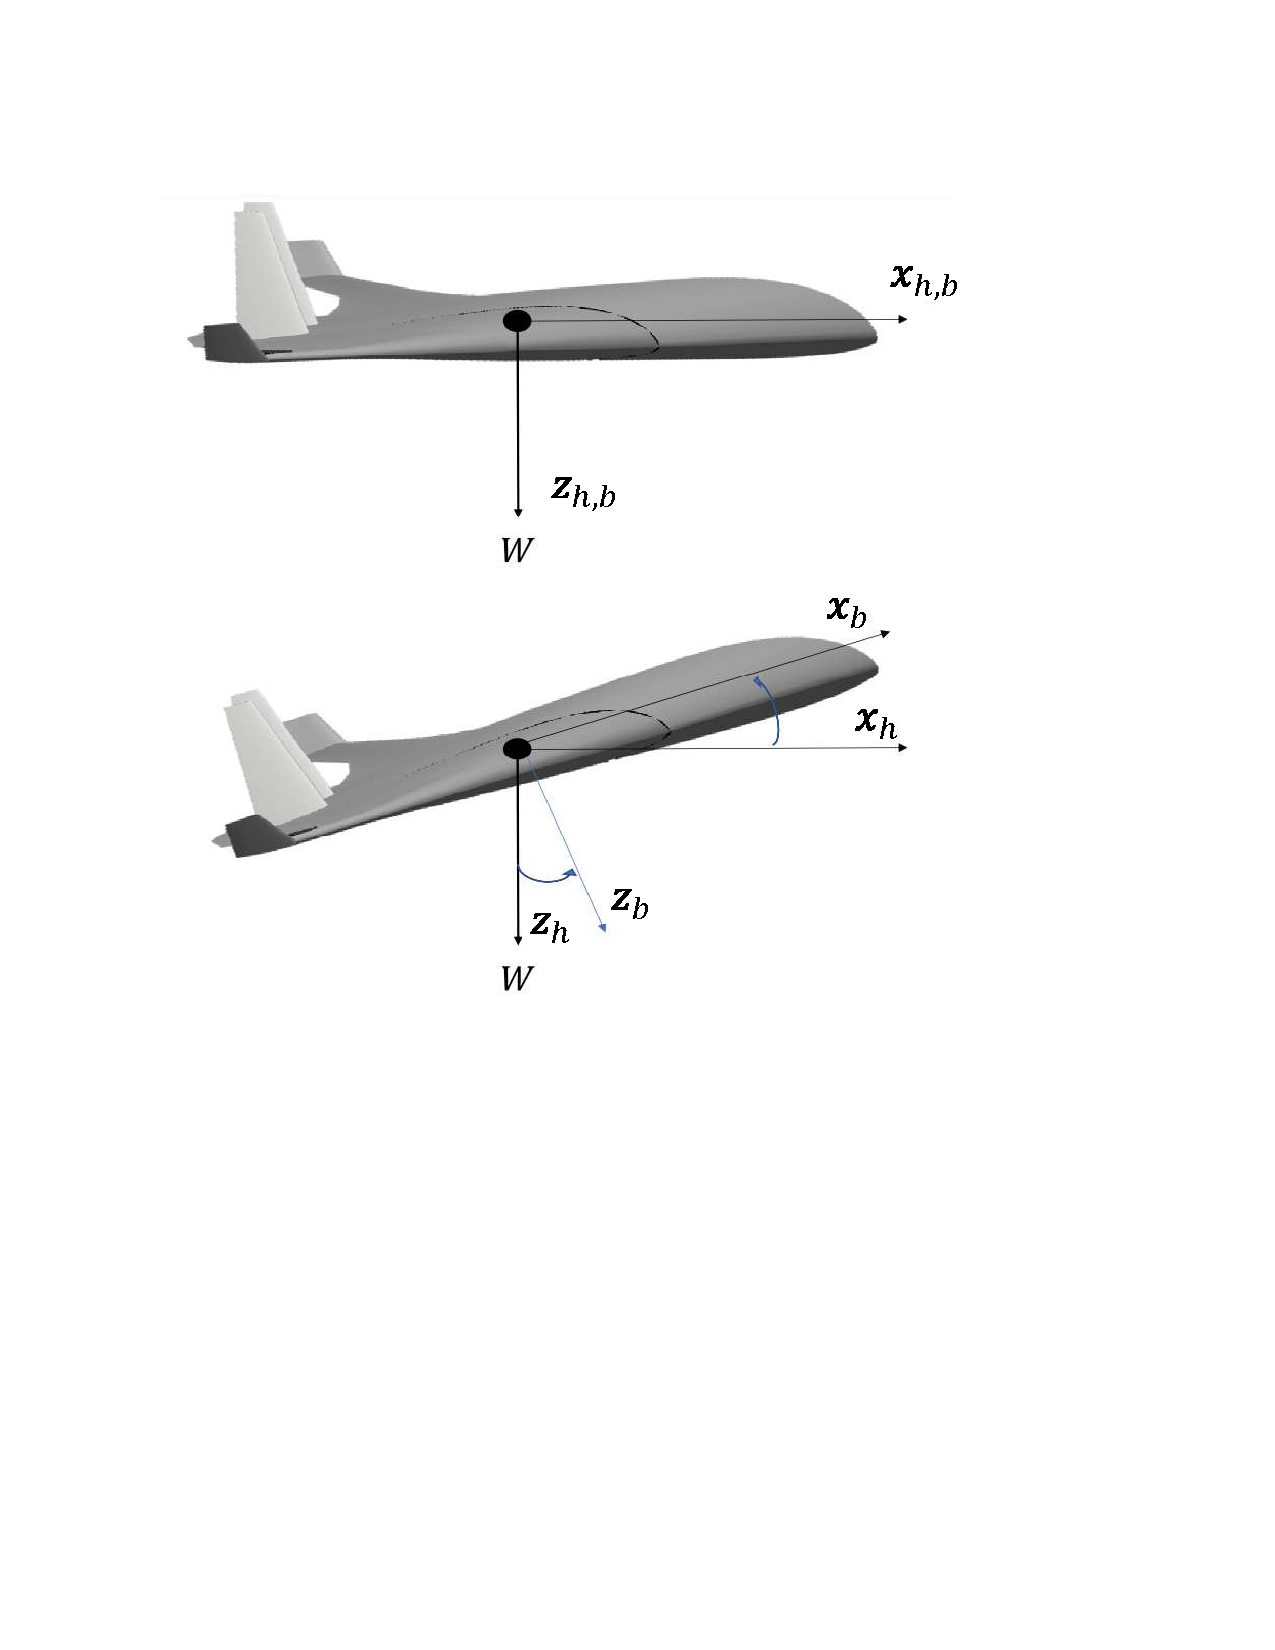
\includegraphics[scale=0.7]{Capitulo3/figs/peso gravedad_cropped (1).pdf}
\caption{Gravitational force in the local horizon plane with respect to the plane body of the aircraft}
\label{fig: fuerza gravitacional}
\end{figure}
In the local horizon plane the gravitational force is represented in the following vector
\begin{gather}
    W_{h}
    =
    \begin{bmatrix}
    0 & 0 & mg 
    \end{bmatrix}^T
\end{gather}
The weight component on the aircraft body axles is found using the matrix of conductor cosines. Use the transformation of the figure \ref{fig: fuerza gravitacional} is a useful reference for the transformation of the aircraft weight into the body plane from the local horizon plane. 
%
Since we assume the body axes and their center gravity as the origin for the gravity components, the contribution corresponding to the moment is zero. $M_G = [0,0,0]^T$, and therefore we will only express gravitational force in the summation of linear forces. 

\begin{gather}
\label{gravedad ec}
    W_{b}
    =
    [S]
    \begin{bmatrix}
    0\\
    0\\
    mg
    \end{bmatrix}
    =
    (mg)
    \begin{bmatrix}
    -S_{\theta}\\
    C_{\theta} S_{\phi}\\
    C_{\theta} C_{\phi} 
    \end{bmatrix}
    =
    \begin{bmatrix}
    X_{G}\\
    Y_{G}\\
    Z_{G}
    \end{bmatrix}_{gravedad}
\end{gather}

therefore

\begin{align}
    X_{G} &= - mg S_{\theta} \\
    Y_{G} &= mg  C_{\theta} S_{\phi}  \\
    Z_{G} &=  mg  C_{\theta} C_{\phi} 
\end{align}

In the equation \ref{gravedad ec} We can appreciate that to obtain the components of gravitational force on the aircraft body axes is multiplied: the mass of the aircraft $m$ by the gravitational constant $g$ by the matrix of cosine directors $[S]$. The gravitational force is all parallel time and its direction coincides with the z axis of the local horizon plane. In the figure \ref{fig: fuerza gravitacional} it is shown that although the orientation of the body axes of the aircraft changed, the direction of the gravitational force remains constant in the direction of the center of gravity towards the center of the earth. Given this nature is that the matrix of cosine directors is applied to preserve these values with respect to the body axes despite the changes in attitude that may exist in the aircraft. It is important to recognize that not all transformations of matrices are orthogonal, but for the case of gravity force, this orthogonal transformation can be applied. 

\bigskip
%%%%%%%%%%%%%%%%%%
\textbf{Propulsion Force}\\
To overcome the inertia of an immobile aircraft, accelerate it in the take-off race, maintain an adequate rate of ascent, achieve a certain speed in cruise flight or simply to overcome the resistance to advance the force of thrust or traction is required. The reaction of the thrust of the engines is of equal intensity but opposite direction (the third law of Newton) to the forward direction that directs the aircraft. The direction of the thrust by convention is usually considered of the same magnitude but direction contrary to the longitudinal body axis of the aircraft, although in reality, the engines usually have a small deviation (1 or 2 degrees Celsius regularly, of longitudinal axis downwards). 

\begin{figure}[h]
    \centering
    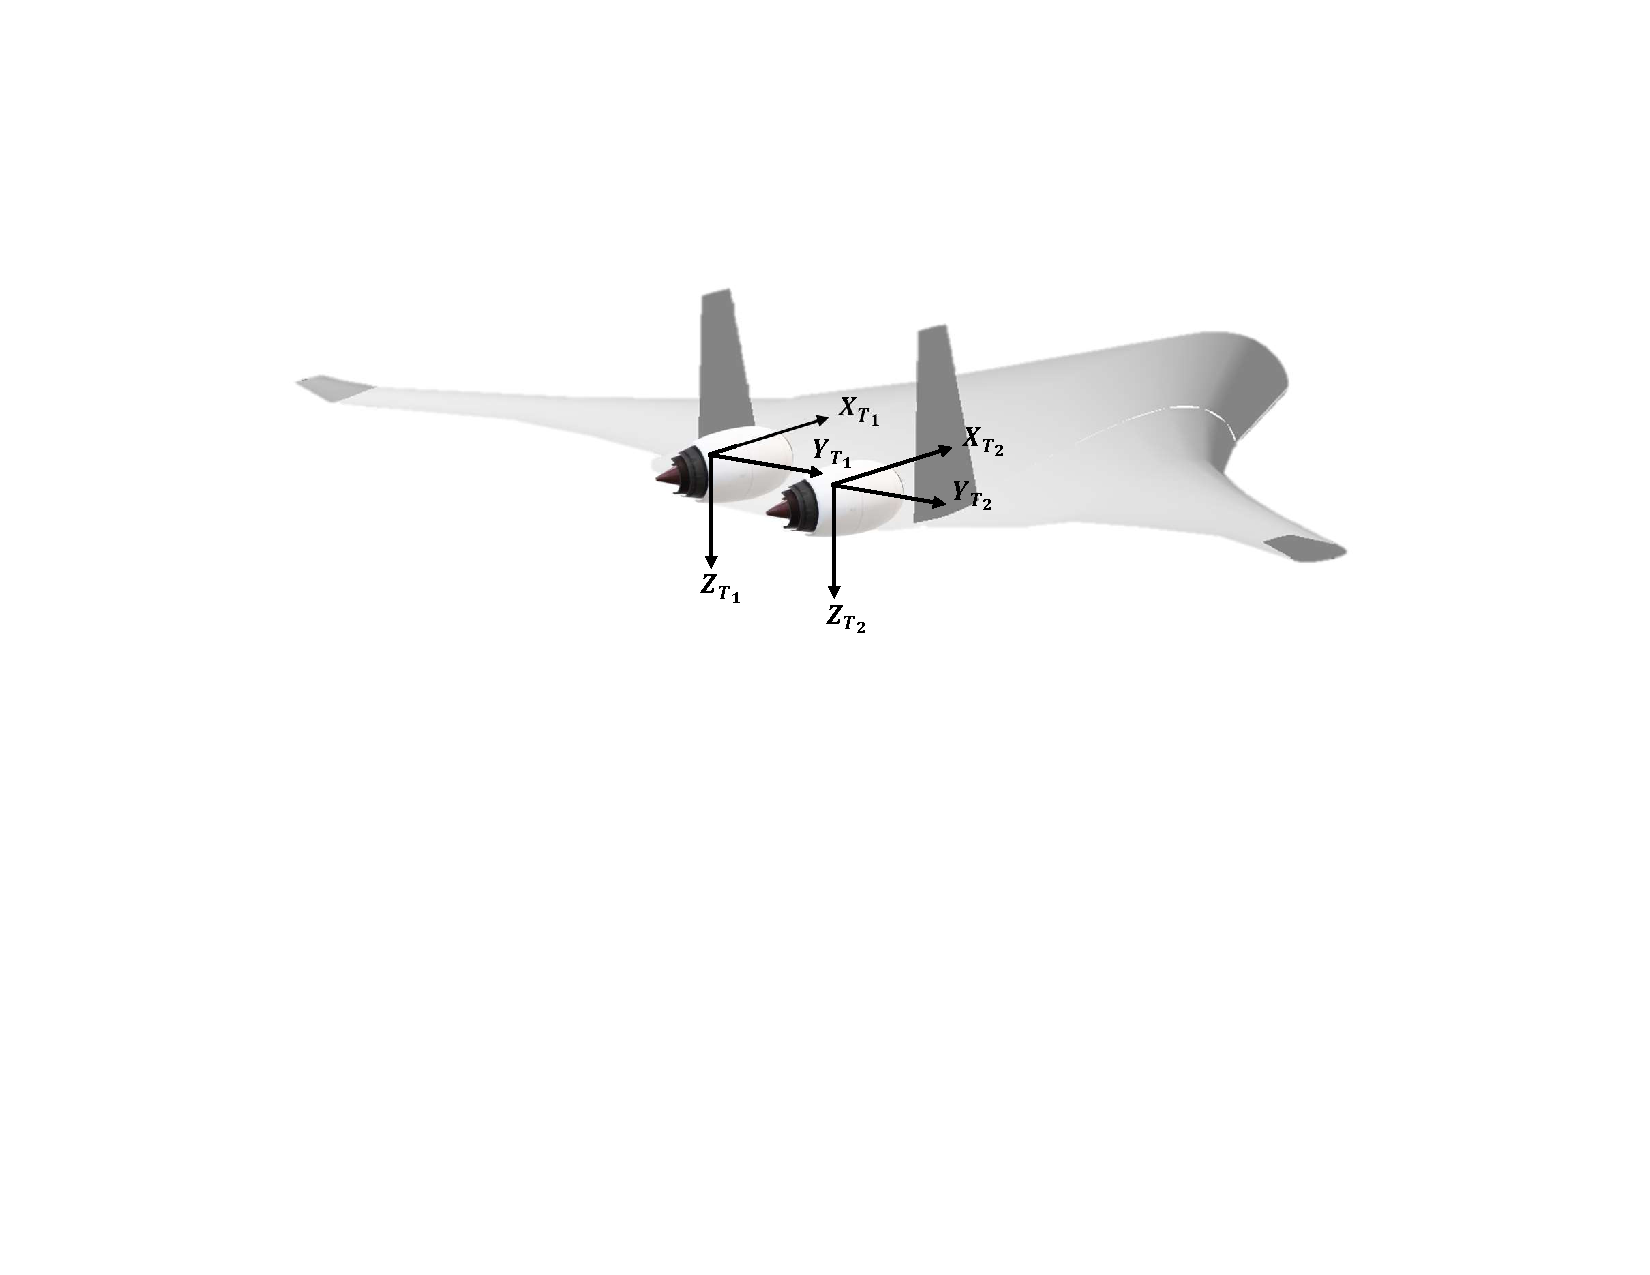
\includegraphics[scale=0.6]{Capitulo3/figs/motores 2_cropped.pdf}
    \caption{Push force}
    \label{Fuerza de empuje}
\end{figure}

The formula for determining the thrust force is defined as
\begin{equation}
    P_T = k_T T_{max}
\end{equation}

where\\
$T_{max}$ is the maximum thrust capable of producing the engine(s). \\
$k_T$ is the coefficient that indicates the percentage of engine power compared to its maximum capacity.

At EHEKATL BWB we have two engines $T_1 , T_2$. According to \cite{USAF1988}, the equations describing the behaviour of the engines on each body axis of the aircraft with respect to the local horizon plane are

\begin{align}
\label{eq motor 1}
    X_{T} &= P_{T1} C_{\theta} C_{\psi} + P_{T2} C_{\theta} C_{\psi} \\
    Y_{T} &= P_{T1}  S_{\psi} + P_{T2}  S_{\psi}  \\
    Z_{T} &= P_{T1}  C_{\psi} S_{\theta} + P_{T2}  C_{\psi} S_{\theta} 
\label{eq motor 2}
\end{align}

\bigskip
%%%%%%%%%%%%%%%%%%%%%%%%%%%%%%%%%%%%%%%%%%%%%%%%%%%%%%%%%%%%%%%%
\textbf{Aerodynamic forces in the aircraft}\\
Two physical mechanisms contribute to produce an aerodynamic force. First, each element of the area surface, multiplied by the pressure relative to its position, results in a normal force element of the aerodynamic profile surface. Second, for each area element on the surface there is a layer of fluid in contact with the surface that does not move relative to the surface. The friction force of the skin will be proportional to the area of the wing surface (area in contact with the fluid). The combination of the pressure force and the friction force of the skin is the resulting aerodynamic force on the supporting surface. \cite{Lewis2016}, ver Figura \ref{fig: sustentacion, arrastre y momento}. 
\begin{figure}[!h]
\centering
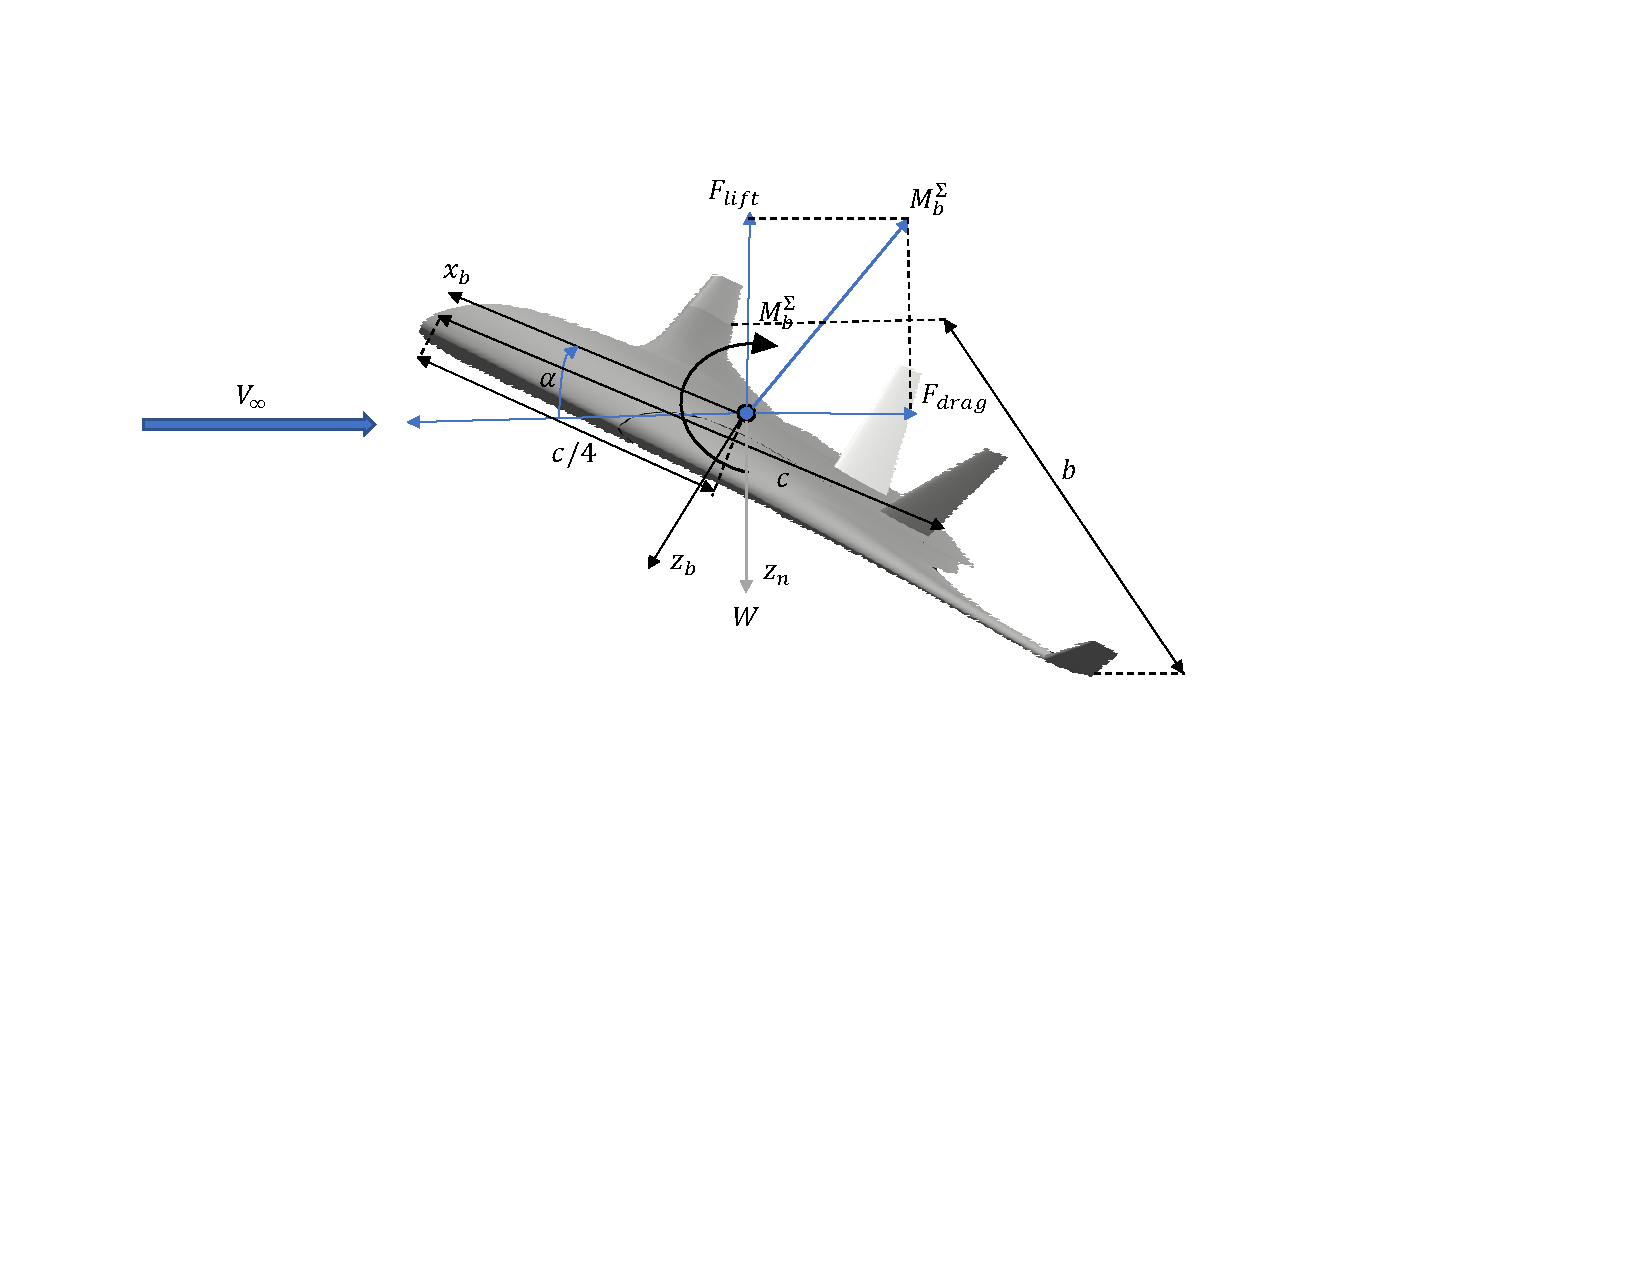
\includegraphics[scale=0.72]{Capitulo3/figs/Best Ehekatl_cropped.pdf}
\caption{Forces of support, drag and moment of pitching in the wind axis}
\label{fig: sustentacion, arrastre y momento}
\end{figure}
The \textbf{Adimensional aerodynamic coefficients} describe the aerodynamic behavior of a wing, wing (supporting surface) or aircraft profile. In addition, they allow the generalization of their performance since by the principle of similarity the results are constant to any scale of greater or lesser proportion. Adimensional aerodynamic coefficients are obtained through simulations, wind tunnel tests and/or flight tests in scale models and have units of 1/rad or 1/degree. The aerodynamic coefficients used in this work are defined as summarizing the basic non-dimensional aerodynamic coefficients, \cite{Mohammad2020}:
\begin{align}
\label{coeficientes adimensionales}
    C_{D} &= C_{D_{0}} + C_{D_{\alpha}} \alpha + C_{D_{q}}q\frac{c}{2U} + C_{D_{\dot \alpha}}\dot \alpha \frac{c}{2U} + C_{D_{u}} \frac{u}{U} + C_{D_{\delta_{e}}}\delta_{e} \\ 
    C_{Y} &= C_{Y_{\beta}}\beta + C_{Y_{p}}p\frac{b}{2U} + C_{Y_{r}}r \frac{b}{2U} + C_{Y_{\delta_{a}}}\delta_{a} + C_{Y_{\delta_{r}}}\delta_{r} \\
    C_{L} &= C_{L_{0}} + C_{L_{0}} \alpha + C_{L_{q}}q\frac{c}{2U} + C_{L_{\dot \alpha}}\dot \alpha \frac{c}{2U} + C_{L_{u}} \frac{u}{U} + C_{L_{\delta_{e}}}\delta_{e} \\
    C_{l} &= C_{l_{\beta}}\beta + C_{l_{p}}p\frac{b}{2U} + C_{l_{r}}r \frac{b}{2U} + C_{l_{\delta_{a}}}\delta_{a} + C_{l_{\delta_{r}}}\delta_{r} \\
    C_{m} &= C_{m_{0}} + C_{m_{\alpha}} \alpha + C_{m_{q}}q\frac{c}{2U} + C_{m_{\dot \alpha}}\dot \alpha \frac{c}{2U} + C_{m_{u}} \frac{u}{U} + C_{m_{\delta_{e}}}\delta_{e} \\
    C_{n} &= C_{n_{\beta}}\beta + C_{n_{p}}p\frac{b}{2U} + C_{n_{r}}r \frac{b}{2U} + C_{n_{\delta_{a}}}\delta_{a} + C_{n_{\delta_{r}}}\delta_{r}
\label{coeficientes adimensionales 2}
\end{align}

Aerodynamic coefficients a-dimensional in \ref{coeficientes adimensionales}-\ref{coeficientes adimensionales 2} contain the \textbf{dimensional stability derivatives}. $ C_{D_{q}}$ for example, describe how the drag force changes $C_D$ in response to the motion variable of the pitching rate $q$. Non-dimensional stability derivatives are important for the design and assessment of the stability and control of an aircraft.

The \textbf{dimensional aerodynamic coefficients} are values that describe the aerodynamic behaviour of an aircraft. Unlike the dimensional coefficients, these values are expressed in physical units and depend on the specific dimensions and characteristics of the aircraft. \ref{Fuerzas y momentos aerodinámicos de la aeronave 2} aerodynamic coefficients are shown where $\bar{q}$ is the \textbf{dynamic pressure} which refers to the kinetic energy of air flow per unit area.
\begin{equation}
    \bar{q} = \frac{1}{2} \rho V^2
\end{equation}
$S$ is the reference area of the supporting surface, $b$ is the size and $c$ It's the central root string.
\begin{table}[!h]
    \centering
    \begin{tabular}{|c|}
    \hline
    \textbf{Aerodynamic Dimensional Stability Coefficients}\\
    \hline
    $X_{A} = \bar{q} S C_{D} (\alpha, V_w, Mach, Re, u, w, q, \delta_e, \delta_T)$ \\
    $Y_{A} = \bar{q} S C_{Y} (\beta, V_w, Mach, Re, v, p, r, \delta_a , \delta_r, \delta_T)$  \\
    $Z_{A} = \bar{q} S C_{L} (\alpha, V_w, Mach, Re, u, w, q, \delta_T)$    \\
    $L_{A} = \bar{q} S b C_{l} (\beta,V_w, Mach, Re, v, p, r, \delta_a , \delta_r, \delta_T)$ \\
    $M_{A} = \bar{q} S c C_{m} (\alpha, V_w, Mach, Re, u, w, q, \delta_T)$  \\
    $N_{A} = \bar{q} S b C_{n} (\beta, V_w, Mach, Re, v, p, r, \delta_a , \delta_r, \delta_T)$  \\
    \hline
    \end{tabular}
    \caption{Aerodynamic forces and moments of the aircraft}
    \label{Fuerzas y momentos aerodinámicos de la aeronave 2}
\end{table}


The \textbf{dimensional stability derivatives} are specific measures of how the aerodynamic forces and moments acting on an aircraft change in response to disturbances in flight conditions. These derivatives are crucial for understanding the stability and control of an aircraft in different situations. The derivatives of longitudinal dimensional stability are related to movement around the lateral axis $y$and describe how the aircraft responds to disturbances at the angle of attack $\alpha$, the pitch rate $q$ and the rate of height variation $\dot{w}$. They are found in the Table \ref{tab:derivadas dimensionales longitudinales}, where $M$ It's Mach's number. 

\begin{table}[!h]
\begin{center}
\caption{Longitudinal Dimensional Stability Derivatives \cite{Etkin1996}}
\begin{tabular}{| c | c | c | }
\hline
\multicolumn{3}{ |c| }{Dimensional Longitudinal Stability Derivatives} \\ 
\hline
$X_u$ & $ - \frac{ \bar{q} S}{mV}(2 C_{D} + M C_{D_{u}})$ & $s^1$ \\
$X_\alpha$ & $ - \frac{ \bar{q} S}{m} (C_L - C_{D_{\alpha}} )$ & $fts^-2 | ms^-2$\\
$X_q$ & $ - \frac{ \bar{q} S}{m} (\frac{c}{2V}  C_{D_{q}}$) & $fts^-2 | ms^-2$ \\ 
$Z_u$ & $ - \frac{ \bar{q} S}{m} (2C_L + M C_{L_{u}}) $ & $s^-1$\\
$Z_\alpha$ & $ - \frac{ \bar{q} S}{m} (C_D + C_{D_{\alpha}})$ & $fts^-2 | ms^-2$\\
$Z_q$ & $ - \frac{ \bar{q} S}{m} ( \frac{c}{2V}  C_{L_{q}} )$ & $fts^-1| ms^-1 $\\
$M_u$ & $ - \frac{ \bar{q} Sc}{I_y V}  (M  C_{m_{u}})$ & $ft^-1s^-1 | m^-1s^-1$\\
$M_\alpha$ & $ - \frac{ \bar{q} Sc}{I_y}  C_{m_{\alpha}}$ & $s^-2$\\
$M_q$ & $ - \frac{\bar{q} Sc}{I_y} (\frac{c}{2V} C_{m_{q}})$ & $s^-1$\\
\hline
\end{tabular}
\label{tab:derivadas dimensionales longitudinales}
\end{center}
\end{table}

Derivatives of lateral-directional dimensional stability are related to movement around the longitudinal axis $x$ and normal axis $z$. Describe how the aircraft responds to disturbances at the sideslip angle $\beta$, the roll rate $p$ and the yaw rate $r$, ver Tabla \ref{tab:derivadas dimensionales laterales}.
\begin{table}[!h]
\begin{center}
\caption{Side-directional dimensional stability derivatives \cite{Etkin1996}}
\begin{tabular}{| c | c | c | }
\hline
\multicolumn{3}{ |c| }{Derivatives of Lateral-Directional Dimensional Stability} \\
\hline
$Y_\beta$ & $ - \frac{\bar{q} S}{m} C_{Y_\beta}$ & $fts^-2 | ms^-2$ \\
$Y_p$ & $ - \frac{ \bar{q} S}{m} (\frac{b}{2V}) C_{Y_p} $ & $fts^-1 | ms^-1$\\
$Y_r$ & $ - \frac{ \bar{q} S}{m} (\frac{b}{2V}) C_{Y_r} $ & $fts^-1 | ms^-1$ \\ 
$L_\beta$ & $ - \frac{ \bar{q}Sb}{I_x} C_{l_\beta} $ & $s^-2$\\
$L_p$ & $ - \frac{\bar{q}Sb}{I_x} (\frac{b}{2V}) C_{l_p} $ & $fts^-1 | ms^-1$\\
$L_r$ & $ - \frac{\bar{q}Sb}{I_x} (\frac{b}{2V}) C_{l_r}  $ & $s^-1$\\
$N_\beta$ & $ - \frac{\bar{q}Sb}{I_x} C_{n_\beta} $ & $s^-2$\\
$N_p$ & $ - \frac{\bar{q}Sb}{I_z} (\frac{b}{2V}) C_{n_p} $ & $s^-1$\\
$N_r$ & $ - \frac{\bar{q}Sb}{I_z} (\frac{b}{2V}) C_{n_r} $ & $s^-1$\\
\hline
\end{tabular}
\label{tab:derivadas dimensionales laterales}
\end{center}
\end{table}

The G constant is related to the lateral-directional stability of the aircraft, which refers to the inertia moments of the aircraft around the main axes of inertia: longitudinal $I_x$, lateral $I_y$ and vertical $I_z$.
\begin{equation}
    G = \frac{1}{[1 - (I_{xz})^2 / (I_x I_z)]}
\end{equation}
\begin{gather}
\label{ld dimensional 1}
    L_\beta ' = G [L_\beta + N_\beta (\frac{I_{xz}}{I_x})] \\
    L_p ' = G [L_p + N_p (\frac{I_{xz}}{I_x})] \\
    L_r ' = G [L_r + N_r (\frac{I_{xz}}{I_x})] \\
    N_\beta ' = G [N_\beta + L_\beta (\frac{I_{xz}}{I_x})] \\
    N_p ' = G [N_p + L_p (\frac{I_{xz}}{I_x})] \\
    N_r ' = G [N_r + L_r (\frac{I_{xz}}{I_x})] \\
\label{ld dimensional 2}
\end{gather}
The stability derivatives shown in \ref{ld dimensional 1}-\ref{ld dimensional 2} take into account additional stability G when there are disturbances. Now, compare $L_\beta$ with $L_\beta'$. the derivative  $L_\beta$ represents undisturbed conditions, while $L_\beta'$ considers the influence of G and lateral-directional coupling. In short, the term G in lateral-directional dimensional stability derivatives introduces a correction to take into account the influence of inertia moments on the lateral-directional stability of the aircraft. These derivatives are those used for simulation purposes. 

\medskip

%%%%%%%%%%%%%%%%%%%%%%%%%%%%%%%%%%%%%%%%%%%%%%%%%%%%%%%%%
\textbf{Aerodynamic Surface Control Forces}\\
Figure \ref{fig: ACS in EHEKATL BWB} sample the aerodynamic control surfaces of the EHEKATL BWB model, which has 8 elevons on the trailing edge (four per semi-wing) and two directional rudders (one pair, one per vertical stabiliser). 

\begin{figure}[!h]
\centering
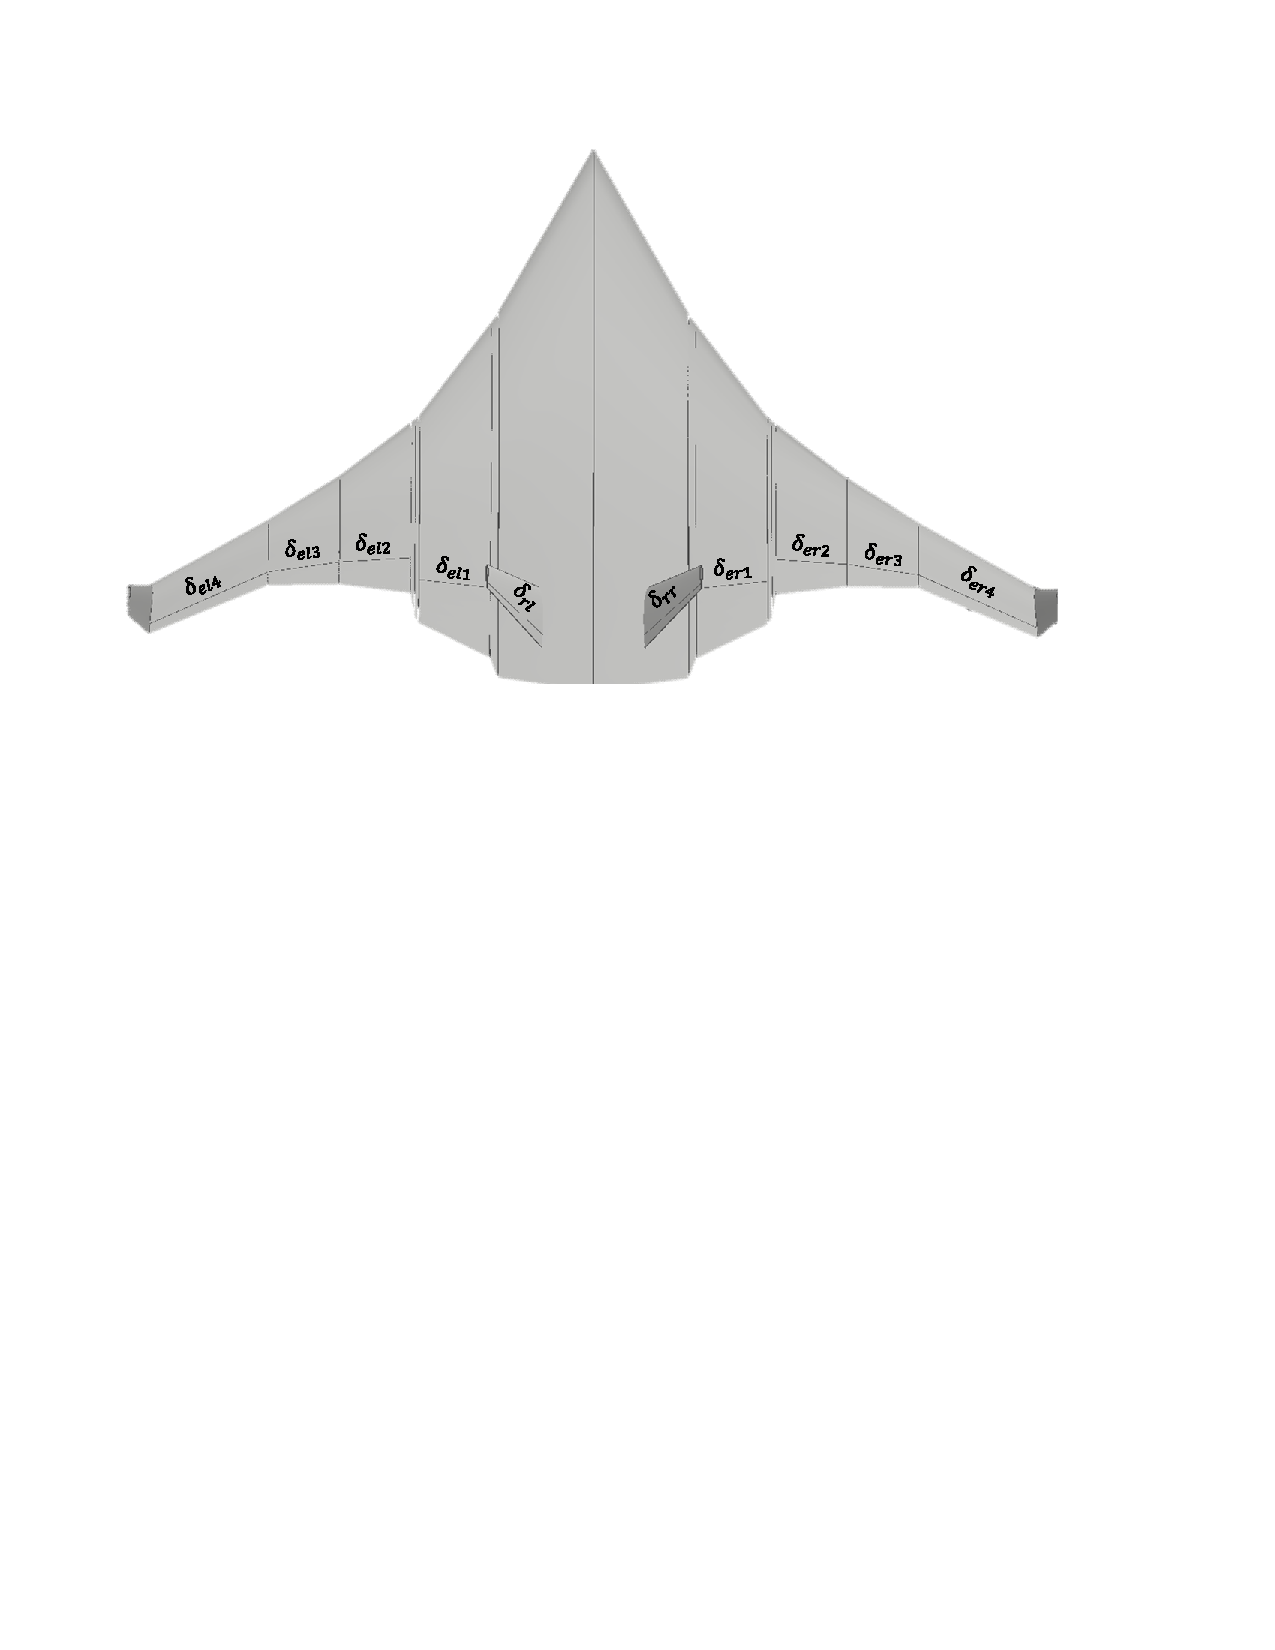
\includegraphics[scale=0.7]{Capitulo3/figs/ehekatl acs_cropped.pdf}
\caption{Aerodynamic control surfaces in EHEKATL BWB}
\label{fig: ACS in EHEKATL BWB}
\end{figure}

There are several ways in which we can configure the moments generated by the ACS at the trailing edge. For a first approximation, and as a basis for the design of drivers for EHEKATL BWB, the conventional control configuration with primary control inputs is set: 
\begin{itemize}
    \item 2 pairs of lifts ($\delta_{e1,e2}$)
    \item 2 pairs of flaps ($\delta_{e3,e4}$)
    \item 1 pair of directional rudder ($\delta_{r}$)
\end{itemize}

%\begin{table}[!h]
%    \centering
%    \begin{tabular}{|c|}
%    \hline
%    \textbf{Coeficientes Aerodinámicos de Control Dimensionales}\\
%    \hline
%     $X_{C} = \bar{q} S C_{D_{\delta_e}} (\alpha, V_w, Mach, Re, \delta_e, \delta_T)$  \\
%     $Y_{C} = \bar{q} S C_{Y_{\delta_a,\delta_r}} (\beta, V_w, Mach, Re, \delta_a , \delta_r, \delta_T)$  \\
%     $Z_{C} = \bar{q} S C_{L_{\delta_e}} (\alpha, V_w, Mach, Re, \delta_e, \delta_T)$   \\
%     $L_{C} = \bar{q} S b C_{l_{\delta_a,\delta_r}} (\beta, V_w, Mach, Re,\delta_a, \delta_r, \delta_T)$ \\
%     $M_{C} = \bar{q} S c C_{m_{\delta_e}} (\alpha, V_w, Mach, Re, \delta_e, \delta_T)$ \\
%    $N_{C} = \bar{q} S b C_{n_{\delta_a,\delta_r}} (\beta, V_w, Mach, Re, \delta_a , \delta_r, \delta_T)$ \\
%    \hline
%    \end{tabular}
%    \caption{Fuerzas y momentos aerodinámicos de la aeronave}
%    \label{Fuerzas y momentos aerodinámicos de la aeronave 3}
%\end{table}

In the aerodynamic coefficients a-dimensional of the aircraft shown in \ref{coeficientes adimensionales}-\ref{coeficientes adimensionales 2} the influence of aerodynamic aerodynamic control coefficients is observed, describing how the aerodynamic moment in an aircraft changes in response to control actions. $C_{m_{\delta_{}e}}$ For example, it describes the behaviour at the pitching moment of the aircraft in response to the deflection movement of the elevators. $\delta_e$. 
%
The aerodynamic coefficients of dimensional control relate the changes in the position or deflection of the ACS of elevators, ailerons and steering rudders with the response in the aircraft's aerodynamic forces and moments, but unlike the dimensional coefficients, these coefficients provide information considering the particular dimensions and characteristics of the aircraft. On the one hand, the derivatives of dimensional longitudinal control refer to the aircraft's response in longitudinal dynamics when the elevators are applied. While the derivatives of lateral-directional control refer to the aircraft's response in lateral-directional dynamics when the alerons and rudders are applied. \ref{tab:derivadas control d} shows the longitudinal and lateral-directional control derivatives dimensional. 
\begin{table}[!h]
\begin{center}
\caption{Dimensional Longitudinal Control Derivatives}
\begin{tabular}{| c | c | c | }
\hline
\multicolumn{3}{ |c| }{Dimensional Longitudinal Control Derivatives} \\ 
\hline
$X_{\delta_e}$ & $ - \frac{\bar{q}S}{m} \frac{\partial C_D}{\partial \delta}$ & $fts^-2 | ms^-2$ \\
$Z_{\delta_e}$ & $ - \frac{\bar{q}S}{m}  \frac{\partial C_L}{\partial \delta}$ & $fts^-2 | ms^-2$ \\
$M_{\delta_e}$ & $ - \frac{\bar{q}Sc}{I_y}  \frac{\partial C_M}{\partial \delta}$ & $s^-2$\\
\hline
\hline
\multicolumn{3}{ |c| }{Dimensional Lateral Control Derivatives} \\
\hline
$Y_{\delta_{a,r}}$ & $ - \frac{\bar{q}S}{m} \frac{\partial C_Y}{\partial \delta}$ & $fts^-2 | ms^-2$\\
$L_{\delta_{a,r}}$ & $ - \frac{\bar{q}Sb}{I_x}  \frac{\partial C_L}{\partial \delta}$ & $s^-2$\\
$N_{\delta_{a,r}}$ & $ - \frac{\bar{q}Sb}{I_z}  \frac{\partial C_n}{\partial \delta})$ & $s^-2$\\
\hline
\end{tabular}
\label{tab:derivadas control d}
\end{center}
\end{table}


Similar to lateral-directional stability derivatives, lateral-directional control derivatives will be transformed considering constant G to consider the perturbations and lateral-directional coupling of the ACS, see equation \ref{eq control ld aaa}. 
\begin{gather}
\label{eq control ld aaa}
    L_{\delta_{a,r}} ' = G [L_\delta + N_\delta (\frac{I_{xz}}{I_x})] \\
    N_{\delta_{a,r}} ' = G [N_\delta + L_\delta (\frac{I_{xz}}{I_x})] \\
\end{gather}

%%%%%%%%%%%%%%%%%%%%%%%%%%%%%%%%%
\section{EHEKATL BWB Model}

Finally, we can establish the set of equations that govern the movement of EHEKATL BWB according to the equations \ref{vh 1} for translational kinematics, \ref{eq cinem rot} for rotational kinematics, \ref{eq dinam tras 1}-\ref{eq dinam tras 2} for translational dynamics and 
\ref{eq: momento angular 1}-\ref{eq: momento angular 2} for rotational dynamics. The above equations define the six-degree coupled flight dynamic model for EHEKATL BWB.

The terms emphasized in blue are the system control inputs according to the Table \ref{tab:derivadas control d} for ACS and \ref{eq motor 1}-\ref{eq motor 2} for the pair of engines; these external forces applied are those that can be regulated to achieve the desired trajectory of the aircraft with the design of controllers.

\medskip

\textbf{Momento lineal traslacional \ref{eq dinam tras 1}-\ref{eq dinam tras 2}}\\
\begin{align}
\label{eq fuerzas ya 1}
    X &= m (\dot u + qw - rv) \\
    Y &= m (\dot v + ru - pw) \\
    Z &= m (\dot w + pv - qu) \\
\label{eq fuerzas ya 2}
\end{align}

Developing applied forces $X,Y,Z$ in accordance with the terms aerodynamics, control, propulsion and gravity we have to 

\begin{align}
    X    &= X_u u + X_{\alpha}\alpha + X_q q + \textcolor{RoyalBlue}{X_{\delta_{e1}} \delta_{e1}}  + \textcolor{RoyalBlue}{X_{\delta_{e2}} \delta_{e2}} + \textcolor{RoyalBlue}{X_{\delta_{T}} \delta_{T}} + X_{G}G \\
    Y &= Y_{\beta} \beta + Y_{p}p + Y_{r} r + \textcolor{RoyalBlue}{Y_{\delta_{a1} \delta_{a1}}} + \textcolor{RoyalBlue}{Y_{\delta_{a2} \delta_{a2}}}  + \textcolor{RoyalBlue}{Y_{\delta_{r}r}} + \textcolor{RoyalBlue}{Y_{\delta_{T} \delta_{T}}} + Y_{G} G \\
    Z &= Z_u u + Z_{\alpha}\alpha + Z_q q + \textcolor{RoyalBlue}{Z_{\delta_{e1}} \delta_{e1}}  + \textcolor{RoyalBlue}{Z_{\delta_{e2}} \delta_{e2}} + \textcolor{RoyalBlue}{Z_{\delta_{T}} \delta_{T}} +  Z_{G}G  \\
\end{align}


\textbf{Momento angular rotacional \ref{eq: momento angular 1}-\ref{eq: momento angular 2}}\\
\begin{align}
\label{eq momentos ya 1}
    L &= \dot p I_{x} + qr(I_{z} - I_{y}) - (\dot r + pq)I_{xz} \\
    M &= \dot q I_{y} + pr(I_{z} - I_{x}) + (p^2 - r^2)I_{xz} \\
    N &= \dot r I_{z} + pq(I_{y} - I_{z}) + (qr - \dot p)I_{xz}
\label{eq momentos ya 2}
\end{align}

Developing applied angular moments $L,M,N$ in accordance with the aerodynamic and control terms we have to

\begin{align}
    L &= L_{p}p + L_{r}r + L_{\beta}\beta + \textcolor{RoyalBlue}{L_{\delta_{a1} \delta_{a1}}} + \textcolor{RoyalBlue}{L_{\delta_{a2} \delta_{a2}}}  + \textcolor{RoyalBlue}{L_{\delta_{r}r}} \\
    M &= M_{u}u + M_{\alpha}\alpha + M_{q}q + \textcolor{RoyalBlue}{M_{\delta_{e1}} \delta_{e1}}  + \textcolor{RoyalBlue}{M_{\delta_{e2}} \delta_{e2}} \\
    N &= N_{p}p + N_{r}r + N_{\beta}\beta + \textcolor{RoyalBlue}{N_{\delta_{a1} \delta_{a1}}} + \textcolor{RoyalBlue}{N_{\delta_{a2} \delta_{a2}}}  + \textcolor{RoyalBlue}{N_{\delta_{r}r}}
\end{align}

\textbf{Linear position \ref{vh 1}}
\begin{align}
\label{posi lineal 1}
    \dot x_H &= u(C_{\psi} C_{\theta}) + v (C_{\psi} S_{\theta} S_{\phi} - S_{\psi} C_{\phi}) + w (C_{\psi} S_{\theta} C_{\phi} + S_{\psi} S_{\phi})  \\
    \dot y_H &= u(S_{\psi} C_{\theta}) + v (S_{\psi} S_{\theta} S_{\phi} + C_{\psi} C_{\phi}) + w (S_{\psi} S_{\theta} C_{\phi} - C_{\psi} S_{\phi})  \\
    \dot z_H &= -u S_{\theta} + v (C_{\theta} S_{\phi}) + w (C_{\theta} C_{\phi}) 
\label{posi lineal 2}
\end{align}


\textbf{Angular position \ref{eq cinem rot}}
\begin{align}
\label{posi angular 1}
    \dot \phi &= p + q (S_{\phi} tan\theta) + r (C_{\phi} tan\theta)\\
    \dot \theta &=  qC_{\phi} - r S_{\phi}\\
    \dot \psi &= q (S_{\phi} sec\theta) + r (C_{\phi} sec\theta)
\label{posi angular 2}
\end{align}

From the equations raised in \ref{eq fuerzas ya 1}-\ref{eq fuerzas ya 2} and  \ref{eq momentos ya 1}-\ref{eq momentos ya 2}, let's clear according to the first-order derivative terms $\dot u, \dot v, \dot w, \dot p, \dot q, \dot r$.


\begin{align}
\label{momento lineal ya 1}
    \dot u &= \frac{1}{m}X - gsen\theta + rv - qw \\
    \dot v &= \frac{1}{m}Y + gcos\theta sen\phi + pw - ru \\
    \dot w &= \frac{1}{m}Z + gcos\theta sen\phi + qu - pv
\label{momento lineal ya 2}
\end{align}

According to \cite{Mohammad2020} given the plane of symmetry also the product of inertia $I_{xz}$ can be considered zero, simplifying angular momentum equations

\begin{align}
\label{moment angu 1 ya}
    \dot p &= \frac{1}{I_x}L + \frac{I_z - I_y}{I_x}qr \\
    \dot q &= \frac{1}{I_y}M  + \frac{I_x - I_z}{I_y}pr \\
    \dot r &= \frac{1}{I_z}N   + \frac{I_y - I_x}{I_z}pq
\label{moment angu 2 ya}
\end{align}

The equations \ref{momento lineal ya 1}-\ref{momento lineal ya 2} are expressed according to the body axes of the aircraft. To transform the wind axes and be able to implement the angle of attack $\alpha$, the sideslip angle $\beta$ and the speed vector $V_T$ the terms are replaced $w$ and $v$ according to the equations \ref{eq: ángulos aerodinámicos con pequeñas perturbaciones}. 

\begin{align}    
\label{aero 1 ya}
    \dot V_T &= \frac{1}{mV}X - \frac{g}{V} sen\theta + r\beta - q\alpha \\
    \dot \beta &= \frac{1}{mV}Y + \frac{g}{V} cos\theta sen\phi + p\alpha - r V_T \\
    \dot \alpha &= \frac{1}{mV}Z + \frac{g}{V} cos\theta sen\phi + q V_T - p\beta
\label{aero 2 ya}
\end{align}

For control and navigation simulations equations are used \ref{posi lineal 1}-\ref{posi lineal 2} to determine the linear position, \ref{posi angular 1}-\ref{posi angular 2} for the angular position,  \ref{moment angu 1 ya}-\ref{moment angu 2 ya} for rotation rate, \ref{momento lineal ya 1}-\ref{momento lineal ya 2} for the rate of translation and \ref{aero 1 ya}-\ref{aero 2 ya} for aerodynamic angles $\alpha$ and $\beta$ and the speed vector $V_T$
\bigskip

%%%%%%%%%%%%%%%%%%%%%%%%%%%%%%%%%%%%%%%%%%%%%%
\textbf{Non Linear Dynamic Longitudinal - 3 GDL}

The equations of the six-degree model of freedom are simplified by decoupling the non-linear longitudinal dynamic, which considers a wing-level flight where lateral-directional velocities $p=r=v=0$. The nonlinear longitudinal dynamics of three degrees of freedom is defined with: the translation on the axis $x$ (advance), the translation on the axis $z$ (altitude) and rotation on the axis $y$ (knocking). 

To model and control the longitudinal dynamics are considered 4 variables of the set of equations: $u, w, q, \theta$. 

%Ecuación de fuerzas aerodinámicas
\begin{align} 
\label{eq: no lineal longitudinal 1}
X &= m (\dot u + qw - rv) \\
Z &= m (\dot w + pv - qu) \\
M &=  \dot q I_{y} + pr(I_{x} - I_{z}) + (p^2 - r^2) I_{xz} \\
\dot \theta &= q C_{\phi} + r S_{\phi}
\end{align}

The longitudinal dynamics of 3 degrees of freedom are observed:

\begin{itemize}
    \item desplazamiento longitudinal $u$
    \item Change of altitude $w$
    \item Angular pitching moment $q$
\end{itemize}

The nodding attitude $\theta$ is a reference variable of the angle formed with respect to the x-axis of the aircraft body with the x-axis of the local horizon plane.
%
When we simplify to obtain the longitudinal non-linear dynamic, unlike the linearization process, it is that the only decoupling criterion is to consider the status variables of the lateral-directional dynamic as zero, i.e. $v=p=r=\phi=\psi=0$. This consideration involves a wing-level flight. By applying this criterion to equations \ref{eq: no lineal longitudinal 1}, We reduce the model as shown in the following equation. 

\begin{align} 
X &= m (\dot u + qw) \\
Z &= m (\dot w - qu) \\
M &=  \dot q I_{y} \\
\dot \theta &= q
\end{align}

Likewise we are negligent with the forces and moments applied by lateral-directional terms, obtaining the terms that only influence longitudinal equations. 

\begin{align}
    X &= X_u u + X_w w  + X_q q + \textcolor{RoyalBlue}{X_{\delta_{e1}} \delta_{e1}}  + \textcolor{RoyalBlue}{X_{\delta_{e2}} \delta_{e2}}+ \textcolor{RoyalBlue}{X_{\delta_{T}} \delta_{T}} + X_G  \\
    Z &= Z_u u + Z_w w + Z_q q + \textcolor{RoyalBlue}{Z_{\delta_{e1}} \delta_{e1}}  + \textcolor{RoyalBlue}{Z_{\delta_{e2}} \delta_{e2}} + \textcolor{RoyalBlue}{Z_{\delta_{T}} \delta_{T}} + Z_G  \\
    M &= M_u u + M_\alpha \alpha + M_q q + \textcolor{RoyalBlue}{M_{\delta_{e1}} \delta_{e1}}  + \textcolor{RoyalBlue}{M_{\delta_{e2}} \delta_{e2}}
\end{align}

The first terms are those of aerodynamic impact, the terms of control and propulsion are highlighted in blue and the last term is of gravitational impact. $\dot w$ o $\dot \alpha$ They are usually small compared to the rest and we can be negligent to them. 

Now we'll clear out the derivatives of the state variables. 

\begin{align} 
\dot u &= \frac{1}{m}X - qw \\
\dot w &= \frac{1}{m}Z + qu \\
\dot q &= \frac{1}{I_{y}}M   \\
\dot \theta &= q
\end{align}

By developing applied longitudinal external forces we obtain all the terms that involve longitudinal dynamics. 

\begin{align} 
\label{eq: modelo longitudinal w}
\dot u &= \frac{1}{m}(X_u u + X_w w + X_q q + \textcolor{RoyalBlue}{X_{\delta_{e1}} \delta_{e1}}  + \textcolor{RoyalBlue}{X_{\delta_{e2}} \delta_{e2}}+ \textcolor{RoyalBlue}{X_{\delta_{T}} \delta_{T}}) - g S_{\theta} - qw \\
\dot w &= \frac{1}{m}(Z_u u + Z_w w + Z_q q + \textcolor{RoyalBlue}{Z_{\delta_{e1}} \delta_{e1}}  + \textcolor{RoyalBlue}{Z_{\delta_{e2}} \delta_{e2}} + \textcolor{RoyalBlue}{Z_{\delta_{T}} \delta_{T}}) + g C_{\theta} + qu \\
\dot q &= \frac{1}{I_{y}}(M_u u + M_\alpha \alpha + M_q q + \textcolor{RoyalBlue}{M_{\delta_{e1}} \delta_{e1}}  + \textcolor{RoyalBlue}{M_{\delta_{e2}} \delta_{e2}})  \\
\dot \theta &= q
\end{align}

The above equations describe the non-linear longitudinal dynamic. We can include the plane of wind axes, which is quite useful and commonly the most used model to know directly in the model the velocity vector and the angle of attack. Another application in the longitudinal dynamic is to consider the flight path variable. 

\begin{figure}[h]
\centering
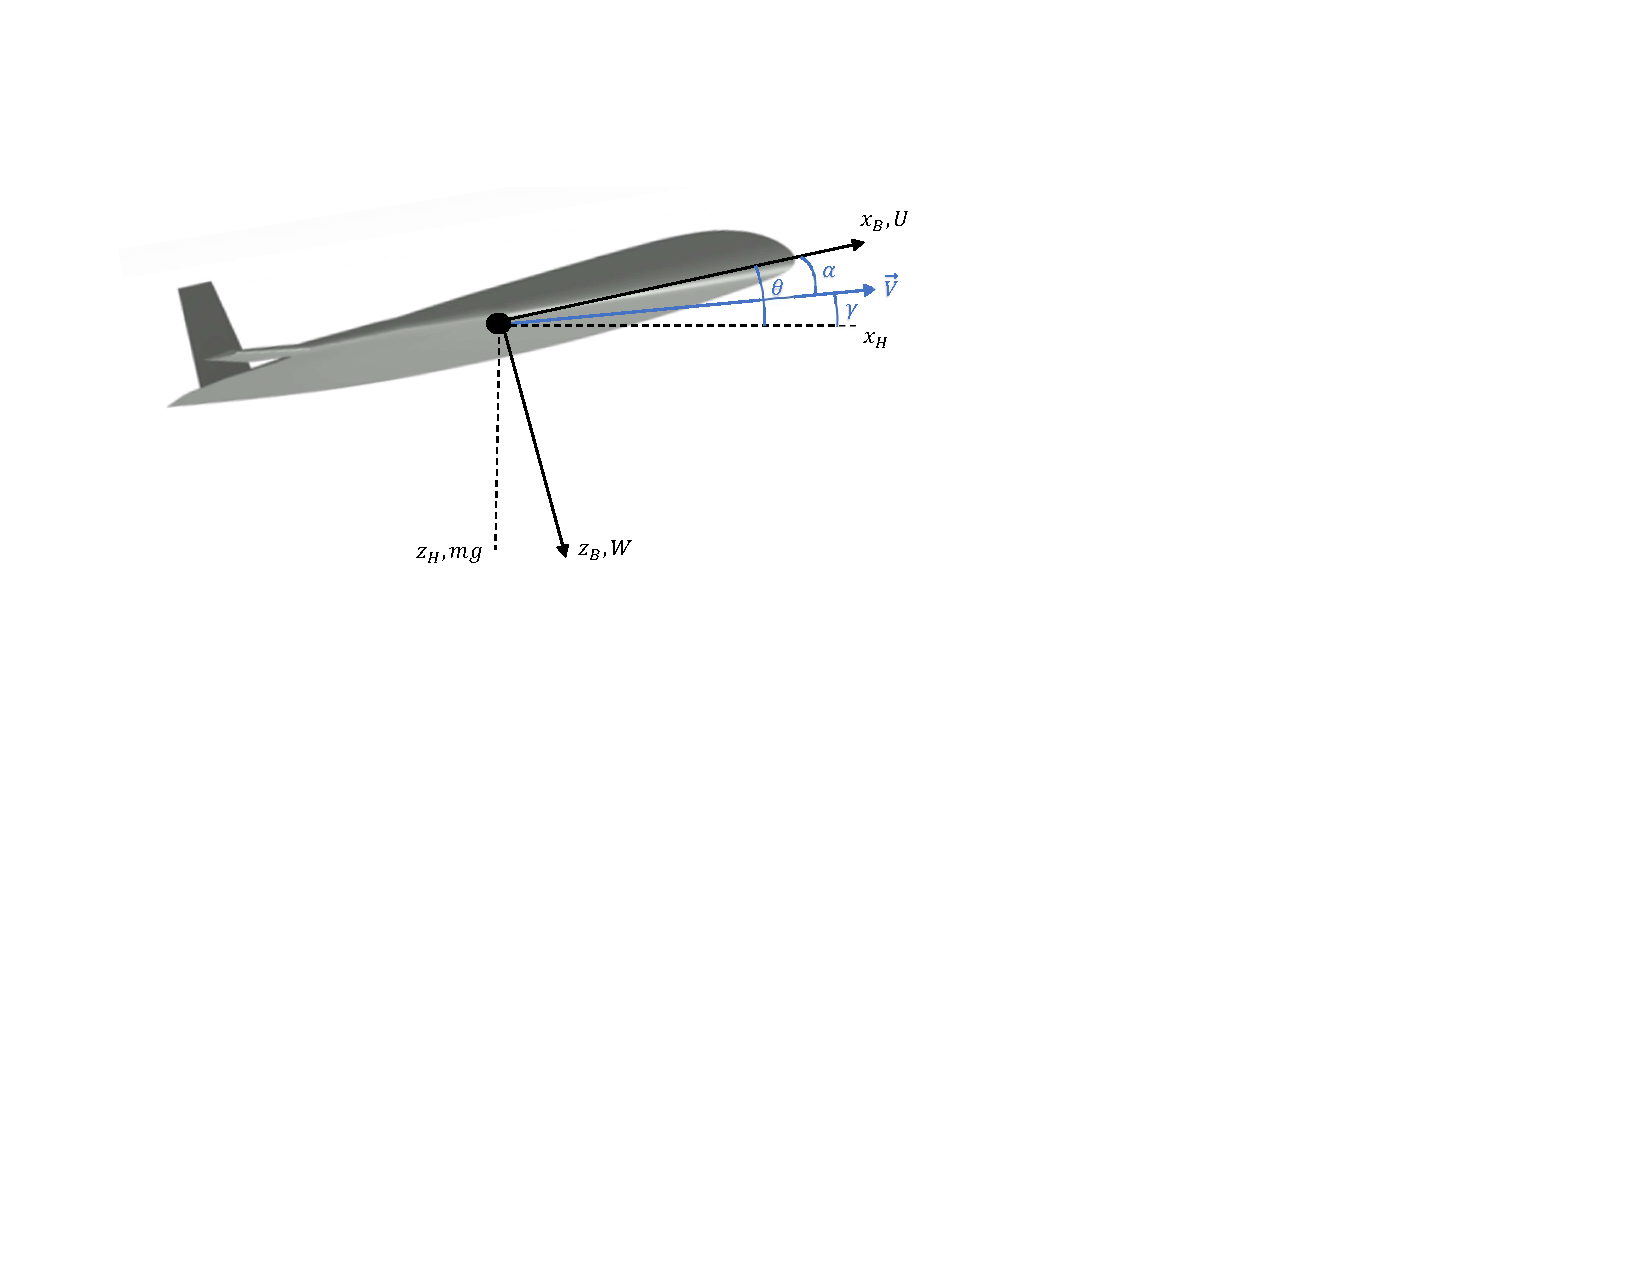
\includegraphics[scale=0.85]{Capitulo3/figs/angulo trayectoria_cropped.pdf}
\caption{flight path, pitch and attack angles in symmetric plane x-z}
\label{fig: ángulos de vuelo, cabeceo y yaw}
\end{figure}

the angle of the flight path is the difference of the pitch angle minus the angle of attack.  

\begin{equation}
\label{eq: trayectoria de vuelo}
    \gamma = \theta - \alpha    
\end{equation}

The transformation of $w$ in $\alpha$ for longitudinal dynamics defines the following longitudinal dynamic system

\begin{align} 
\label{eq: modelo longitudinal alpha}
\dot V_T &= \frac{1}{mV}(X_u u + X_\alpha \alpha + X_q q + \textcolor{RoyalBlue}{X_{\delta_{e1}} \delta_{e1}}  + \textcolor{RoyalBlue}{X_{\delta_{e2}} \delta_{e2}}+ \textcolor{RoyalBlue}{X_{\delta_{T}} \delta_{T}}) - \frac{g}{V} S_{\theta} - q \alpha \\
\dot \alpha &= \frac{1}{mV}(Z_u u + Z_\alpha \alpha + Z_q q + \textcolor{RoyalBlue}{Z_{\delta_{e1}} \delta_{e1}}  + \textcolor{RoyalBlue}{Z_{\delta_{e2}} \delta_{e2}} + \textcolor{RoyalBlue}{Z_{\delta_{T}} \delta_{T}}) + \frac{g}{V} C_{\theta} + qu \\
\dot q &= \frac{1}{I_{y}}(M_u u + M_\alpha \alpha + M_q q + \textcolor{RoyalBlue}{M_{\delta_{elev_{i}}} \delta_{elev_{int}}}  + \textcolor{RoyalBlue}{M_{\delta_{T \Theta}} \delta_{T \Theta}})  \\
\dot \theta &= q
\end{align}

In order to include the flight path in the longitudinal dynamics, the \ref{eq: trayectoria de vuelo} in \ref{eq: modelo longitudinal alpha} last non-linear longitudinal modeling

\begin{align} 
\label{eq: modelo longitudinal gamma}
\dot V_T &= \frac{1}{mV}(X_u u + X_\alpha \alpha + X_q q + \textcolor{RoyalBlue}{X_{\delta_{elev_{i}}} \delta_{elev_{i}}}  + \textcolor{RoyalBlue}{X_{\delta_{T \Theta}} \delta_{T \Theta}}) - \frac{g}{V} S_{\theta} - q \alpha \\
\dot \gamma &= -\frac{1}{mV}(Z_u u + Z_\alpha \alpha + Z_q q + \textcolor{RoyalBlue}{Z_{\delta_{elev_{i}}} \delta_{elev_{i}}} + \textcolor{RoyalBlue}{Z_{\delta_{T \Theta}} \delta_{T \Theta}}) - \frac{g}{V} C_{\theta} \\
\dot q &= \frac{1}{I_{y}}(M_u u + M_\alpha \alpha + M_q q + \textcolor{RoyalBlue}{M_{\delta_{elev_{i}}} \delta_{elev_{int}}}  + \textcolor{RoyalBlue}{M_{\delta_{T \Theta}} \delta_{T \Theta}}) \\
\dot \alpha &= q - \dot \gamma 
\end{align}


Any of the three non-linear longitudinal dynamic models can be used depending on the variables we seek to obtain or the particular control application we want to employ. 

\bigskip
%%%%%%%%%%%%%%%%%%%%%%%%%%%%%%%%%%%%%%%%%%%%%%
\textbf{Non-Linear Lateral-Directional Dynamic Model - 3 GDL}\\
Now we will simplify the equations of the six degree model of freedom decoupled the lateral-directional dynamics, which considers three degrees of freedom: the translation on the axis $y$ (side displacement), rotation on the axis $x$ (roll) and rotation on the axis $z$ To model and control the non-linear lateral-directional dynamics, 4 variables of the set of equations are considered: $v, p, r, \phi$. 


\begin{align} 
Y &= m (\dot v + ru - pw) \\
L &= \dot p I_x + \dot r I_{xz} + qr(I_z - I_y) - pq I_{xz} \\
N &=  \dot r I_z + \dot p I_{xz} + pq(I_y - I_x) + qr I_{xz}  \\
\dot \phi &= p + (q S_{\phi} + r C_{\phi}) tan_{\theta}
\end{align}

The lateral-directional dynamics of 3 degrees of freedom are observed: 
\begin{itemize}
    \item desplazamiento lateral $v$
    \item angular moment of roll $p$
    \item Angular moment of yaw $r$
\end{itemize}

The variable of the roll attitude $\phi$ is a reference for the level of the wing of the aircraft, through the transformation of the axle $y$ of the aircraft body in respect of the axle $y$ The simplification process for the non-linear lateral-directional dynamic is somewhat more complex than the longitudinal one, since we cannot zero the values of attitude to the pitching $\theta_{e}$, altitude $w_{e}$ and speed $u_{e}=V_{T}$, instead we must consider these constant values regarding the condition of flight in balance, hence the suffix $e$. The equations of angular dynamics are simplified according to $q=0$ and \cite{Mohammad2020} considering the product of inertia $I_{xz}=0$. 

\begin{align} 
Y &= m (\dot v - u_{e}*r + w_{e}*p)\\
L &= \dot p I_x \\
N &=  \dot r I_z \\
\dot \phi &= p + r C_{\phi} tan_{\theta_{e}}
\end{align}

In the same way, we will be negligent with the external linear and angular forces applied in longitudinal dynamics, obtaining the terms of the forces that have interference in lateral-directional dynamics. 

\begin{align}
    Y &= Y_{v} v + Y_{p}p + Y_{r} r + \textcolor{RoyalBlue}{Y_{\delta_{T} \delta_{T}}} + \textcolor{RoyalBlue}{Y_{\delta_{a1} \delta_{a1}}} + \textcolor{RoyalBlue}{Y_{\delta_{a2} \delta_{a2}}}  + \textcolor{RoyalBlue}{Y_{\delta_{r}r}} + Y_{G} G \\
    L &= L_{p}p + L_{r}r + L_{v}v + \textcolor{RoyalBlue}{L_{\delta_{a1} \delta_{a1}}} + \textcolor{RoyalBlue}{L_{\delta_{a2} \delta_{a2}}}  + \textcolor{RoyalBlue}{L_{\delta_{r}r}} \\
    N &= N_{p}p + N_{r}r + N_{v}v + \textcolor{RoyalBlue}{N_{\delta_{a1} \delta_{a1}}} + \textcolor{RoyalBlue}{N_{\delta_{a2} \delta_{a2}}}  + \textcolor{RoyalBlue}{N_{\delta_{r}r}}
\end{align}


Now let's clear with respect to the derivatives of the status variables. 

In the general equation we get

\begin{align}
    \dot v & = \frac{1}{m}Y - u_{e} r + w_{e} p \\
    \dot p & = \frac{1}{I_x}L \\
    \dot r & = \frac{1}{I_z}N \\
    \dot \phi &= p + r C_{\phi} tan_{\theta_{e}}
\end{align}

By developing lateral-directional forces in non-linear dynamics we obtain the following equations. 

\begin{align}
    \dot v & = \frac{1}{m}(Y_{v} v + Y_{\dot v}\dot v + Y_{p}p + Y_{r} r + \textcolor{RoyalBlue}{Y_{\delta_{T} \delta_{T}}} + \textcolor{RoyalBlue}{Y_{\delta_{a1} \delta_{a1}}} + \textcolor{RoyalBlue}{Y_{\delta_{a2} \delta_{a2}}}  + \textcolor{RoyalBlue}{Y_{\delta_{r}r}}) + gC_{\theta}S_{\phi} - u_{e}r + w_{e}p  \\
    \dot p & = \frac{1}{I_x}(L_{p}p + L_{r}r + L_{v}v + L_{\dot v}\dot v + \textcolor{RoyalBlue}{L_{\delta_{a1} \delta_{a1}}} + \textcolor{RoyalBlue}{L_{\delta_{a2} \delta_{a2}}}  + \textcolor{RoyalBlue}{L_{\delta_{r}r}}) \\
    \dot r & = \frac{1}{I_z}(N_{p}p + N_{r}r + N_{v}v + N_{\dot v}\dot v + \textcolor{RoyalBlue}{N_{\delta_{a1} \delta_{a1}}} + \textcolor{RoyalBlue}{N_{\delta_{a2} \delta_{a2}}}  + \textcolor{RoyalBlue}{N_{\delta_{r}r}})\\
    \dot \phi &= p + r C_{\phi} tan_{\theta_{e}}
\end{align}

The above equations describe the lateral-directional non-linear dynamics in the plane body of the aircraft. To consider within this model the velocity vector defined in the plane of wind, we take the consideration  \ref{eq: ángulos aerodinámicos con pequeñas perturbaciones} and clear the interest variable $\beta$ getting the next model. 

\begin{align}
    \dot \beta & = \frac{1}{mV}(Y_{\beta} \beta + Y_{p}p + Y_{r} r +   \textcolor{RoyalBlue}{Y_{\delta_{T} \delta_{T}}} + \textcolor{RoyalBlue}{Y_{\delta_{a1} \delta_{a1}}} + \textcolor{RoyalBlue}{Y_{\delta_{a2} \delta_{a2}}}  + \textcolor{RoyalBlue}{Y_{\delta_{r}r}}) + \frac{g}{V}C_{\theta}S_{\phi} - u_{e}r + w_{e}p  \\
    \dot p & = \frac{1}{I_x}(L_{p}p + L_{r}r + L_{\beta}\beta + L_{\dot \beta}\dot \beta + \textcolor{RoyalBlue}{L_{\delta_{a1} \delta_{a1}}} + \textcolor{RoyalBlue}{L_{\delta_{a2} \delta_{a2}}}  + \textcolor{RoyalBlue}{L_{\delta_{r}r}}) \\
    \dot r & = \frac{1}{I_z}(N_{p}p + N_{r}r + N_{\beta}\beta + N_{\dot \beta}\dot \beta + \textcolor{RoyalBlue}{N_{\delta_{a1} \delta_{a1}}} + \textcolor{RoyalBlue}{N_{\delta_{a2} \delta_{a2}}}  + \textcolor{RoyalBlue}{N_{\delta_{r}r}})\\
    \dot \phi &= p + r C_{\phi} tan_{\theta_{e}}
\end{align}


\section{Discussion}

The proper selection of reference systems is essential to accurately describe the movement and orientation of aircraft during flight. The chosen reference systems provide an essential framework for analysis of kinematics and dynamics, and have a significant impact on the formulation of motion equations.

The kinematic analysis allows the mathematical description of the position, speed and acceleration of the EHEKATL BWB according to time. This section provides the basis for understanding and predicting the behaviour of the aircraft in flight, considering variables such as orientation, translation and rotation.

Formulation of dynamic equations is essential to understand how external forces and moments affect aircraft movement. Analysis of the forces and moments involved provides crucial information for the stability, control and performance of EHEKATL BWB.

The study of applied forces and moments considers interactions with the environment during flight, considering the aerodynamic, gravity, propulsion and control forces; and how the aircraft responds to the application of these forces. Detailed understanding of these aspects is essential for the design of effective control systems and flight safety.

The dynamic model of the EHEKATL BWB aircraft in terms of defining stability and control parameters, status and control variables, and motion equations; it is the culmination of this chapter. The dynamic model provides a basic tool for simulation and prediction of the aircraft's behavior in a wide range of flight conditions.

The dynamic analysis and modelling presented in this chapter form the basis for the implementation of control systems and performance assessment of the EHEKATL BWB aircraft.

In the appendices section \ref{linealizacion a} the linearization process is developed according to the six degree freedom movement equations, and the longitudinal linear model and the lateral-directional linear model are decoupled in the same way.





%%%%%%%%%%%%%%%%%%%%%%%%%%%%%%%%%%%%%%%%%%%%%%%%%%%%%%%%%%%%%%%%%%%%%%%%%
%                        Sistemas de Control de Vuelo (FCS)     %
%%%%%%%%%%%%%%%%%%%%%%%%%%%%%%%%%%%%%%%%%%%%%%%%%%%%%%%%%%%%%%%%%%%%%%%%%
\chapter{Design of Controllers}

The controller design is a discipline within aerospace engineering that focuses on the development of control systems to stabilize and control the movement of aerial vehicles, space vehicles and rockets. A flight controller is an electronic system that uses acceleration, speed and position sensors to determine the trajectory of both manned and unmanned vehicles. The controller generates a reference command (may be manual, issued by a pilot; or automatic, issued by a computer) and in response to this reference command (also known as a track signal or desired trajectory) act the vehicle's control inputs to achieve or reach the desired state from a previous state or initial condition.In the case of EHEKATL BWB, primary control inputs (elevators, spoilers, rudders and engines) were established to control their movement. The main objective of the flight controller is to ensure that the aircraft flies in a stable and predictable manner, responding to the pilot's commands or following a specific trajectory autonomously.

The flight controllers are structured into two parts: the measurement system and the control system. The measurement system uses sensors to measure aircraft variables such as speed, altitude, attitude and orientation. These data are processed in the control system that uses algorithms to calculate the commands needed to keep the aircraft in its desired path. These commands are sent to actuators who are responsible for moving control effectors, such as engines and aerodynamic control surfaces.

There are two types of flight controllers: linear and non-linear. Linear controllers are control systems that use linear equations. These controllers are simple and easy to implement, but are restricted to an operating range and may not be able to handle certain disturbances outside of their equilibrium point. 

On the other hand, non-linear controllers try to compensate for highly non-linear dynamics and their objective is to compensate for this dynamic by means of robust and model-free controllers, especially in aircraft which are subject to various types of disturbances or states that require a higher degree of freedom and manoeuvrability. The choice between a linear or non-linear controller depends on the specific application and characteristics of the vehicle. In short, the design of flight controllers is essential to ensure that an aircraft flies ensuring certain operating conditions and stability.  

In this chapter, the non-linear flight controllers Backstepping and Adaptive Backstepping for EHEKATL BWB are developed. Aerodynamic parameters are obtained with XFLR5, where for flight simulations a specific operating point or time point is used, being then simulations of systems invariant over time. The design and simulation of flight controllers is performed in the programming language PYTHON.


%%%%%%%%%%%%%%%%%%%%%%%%%
 \section{Backstepping}

One method introduced and used to explore new directions in systems control design with non-linear dynamics is Backstepping. 
%
Backstepping controllers synthesize a complex non-linear dynamic system (aircraft) into interconnected subsystems. Therefore, the aircraft dynamic system is divided into a series of subsystems.
%
The objective of control with Backstepping is to achieve by cascades the overall control of these subsystems, starting with the last subsystem. The output of the controller becomes the input of the next subsystem, and the continuous process until reaching the first subsystem. 
%
Each controller subsystem is designed to stabilize and track the desired path of that subsystem. 
%
The Backstepping controller is designed to stabilize and control the aircraft’s dynamics. We can systematically build controllers that handle the complex dynamics and non-linearities of the aircraft’s movement, in addition to ensuring stability, \cite{vanGils2015}. 

The Backstepping drivers for EHEKATL BWB are:
\begin{itemize}
    \item 3-GDL Longitudinal Backstepping Controller 
    \item Bacsktepping side-directional 3-GDL controller
\end{itemize}

With Backstepping we can have a single lateral-directional controller that considers the nonlinearities and lateral-directional coupling according to the response signal of the wings and rudders. 

\medskip

%%%%%%%%%%%%%%%%%%%%%%%%%%%%%%%%%%%%%%%%%%%%
\textbf{Backstepping Controller}\\
For EHEKATL BWB Backstepping Controllers, the following structure is used for representation of the non-linear dynamic model in state space.

\begin{align}
\label{estructura backstepping 1}
    \dot x_{1} &= f_{1} + g_1 x_2 + h_1 u \\ \nonumber
    \dot x_{2} &= f_{2} + g_2 u
\end{align}

The equation \ref{estructura backstepping 1} allows to represent the non-linearities of the coupled movement (between linear and angular speeds) in the product of $g_1 x_2$, while allowing to show the participation of control entries in both subsystems. 

Estimation errors are defined $z_1, z_2$ as the difference between status variables ($x_1, x_2$) and the desired follow-up signals ($x_1^d, x_2^d$) The error $z_3$ considers the dynamics of the actuators, and is defined as the difference between the actual control input $u$ and the reference command $u^d$.

\begin{align}
    z_1 &= x_1 - x^d_1 \\
    z_2 &= x_2 - x^d_2 \\
    z_3 &= u - u^d
\end{align}

The function of transferring the dynamics of actuators is defined on the basis of a delay of the first order: 

\begin{equation}
    \dot u = - \frac{1}{\tau}u + \frac{1}{\tau} u_c
\end{equation}

where: $\tau$=tiempo constante, $u_{c}$= control command generated by the controller and $u$= real dynamic command of actuators. 

A candidate function of Lyapunov is proposed for each of the estimation errors defined in the previous step.

\begin{gather}
\label{Lyapunovn 1}
    V (z_1, z_2, z_3) =\frac{1}{2} z^T_1 z_1 + \frac{1}{2} z^T_2 z_2 + \frac{1}{2} z^T_3 z_3
\end{gather}

 The proposed candidate role of Lyapunov in \ref{Lyapunovn 1}.

\begin{align}
       \dot V &= z^T_1 \dot z_1 + z^T_2 \dot z_2 + z^T_3 \dot z_3 \nonumber \\
        &= z^T_1 (\dot x_1 - \dot x^d_1) + z^T_2 (\dot x_2 - \dot x^d_2) + z^T_3 (\dot u - \dot u^d) \nonumber \\ 
    &= z^T_1 (f_1 + g_{1} x_2 + h_1 u - \dot x^d_1) + z^T_2 (f_2 + g_{2} u - \dot x^d_2) + z^T_3 (\frac{1}{\tau}(u_c - u) - \dot u^d) \nonumber \\
    &= z^T_1 (f_1 + g_{1} (z_2 + x_{2}^d) + h_1 (z_3 + u^d) - \dot x^d_1) + z^T_2 (f_2 + g_{2} (z_3 + u^d) - \dot x^d_2)\nonumber \\
    &+ z^T_3 (\frac{1}{\tau}(u_c - u) - \dot u^d)
\end{align}

Remembering the error $z_2 = x_2 - x^d_2$ is easily obtained $x_2 = z_2 + x^d_2$ for the first subsystem, while for the second subsystem we have to $z_3 = u - u^d$, and therefore $u = z_3 + u^d$. 

Once the derivative of Lyapunov's candidate function has been developed, virtual control laws are proposed in order to compensate for the resulting terms and add the term control $k_n z_n$. The term control is composed of a profit matrix $k_n$ known and defined as a positive constant, which multiplies squared of the estimation error $z_n$. The purpose of the control term is to obtain a damping or dissipation until the desired value of the tracking signal or reference command is reached. 

\begin{align}
\label{leyes de control 1}
    x^d_2 &= \frac{1}{g_{1}} [- f^T_1 + \dot x^d_1 - k_1 z_1] \nonumber \\
    u^d &= \frac{1}{g_{2}} [-f_{2}^T + \dot x_{2}^d - k_2 z_2 - g_{1}^T z_1] \nonumber \\
    u_c &= u + \tau [\dot u^d - g_{2}^T z_2 - (h_1^T u + h_{1}^T) z_1 - k_3 z_3]
\end{align}

The virtual control laws are now replaced \ref{leyes de control 1} in the derivative of Lyapunov's candidate function and develops.

\begin{align}
      \dot V &=  z^T_1 (f_1 + g_{1} (z_2 + [\frac{1}{g_{1}} [- f^T_1  + \dot x^d_1 - k_1 z_1]]) + h_1 z_3 + h_1 u - \dot x^d_1) \nonumber \\
      &+ z^T_2 (f_2 + g_{2} (z_3 + [\frac{1}{g_{2}} [-f_{2}^T + \dot x_{2}^d - k_2 z_2 - g_{1}^T z_1]]) - \dot x^d_2) \nonumber \\
      &+ z^T_3 (\frac{1}{\tau}([ u + \tau [\dot u^d - g_{2}^T z_2 - u h_1^T z_1 - h_{1}^T z_1 - k_3 z_3]] - u) - \dot u^d)
\end{align}

Entonces,

\begin{align}
    &= z^T_1 (g_1 z_2  + h_1 z_3 + h_1 u - k_1 z_1) + z^T_2 (g_2 z_3 - g^T_1 z_1 - k_2 z_2) \nonumber \\
      &+ z^T_3 (- u h_1^T z_1 - h_1^T z_1  - g_{2}^T - k_3 z_3) \nonumber \\
      &= (z^T_1g_1 z_2 - z^T_2 g^T_1 z_1 ) + (z_1^T(h_1 (z_3 + u)) - h_1^T(z_1(1+u))) \nonumber \\
      &- z^T_1 k_1 z_1 + (z^T_2 g_2 z_3 - z^T_3 g_{2}^T z_2 ) -  z^T_2 k_2 z_2 - z^T_3  k_3 z_3 \nonumber \\
      &= - z^T_1 k_1 z_1 - z^T_2 k_2 z_2 -  z^T_3  k_3 z_3
\label{backstepping eq}
\end{align}

it is observed that the proposed virtual control laws correctly offset the required terms. After applying the virtual control laws, the derivative of Lyapunov’s candidata function is defined: 

\begin{equation}
\label{Lyapunov sss}
    \dot V = - z^T_1 k_1 z_1 - z^T_2 k_2 z_2 -  z^T_3  k_3 z_3
\end{equation}

and therefore: 

\begin{gather}
    \dot V \leqslant 0
\end{gather}

According to the La Salle-Yoshizawa theorem, the states $z_1,z_2,z_3$ converge asymptotically to the origin as  $t\to\infty$This is it, $z_1=z_2 = z_3 \to 0$ which implies that $x_1\to x_1^d$, $x_2\to x_2^d$ and $u\to u^d$. In addition with the equation \ref{Lyapunov sss} We have to $z_1, z_2, z_3 \in L_2$. 

%Lyapunov introdujo la idea de una función de energía ficticia, denominada función de Lyapunov, aplicable a cualquier ecuación diferencial y tanto para sistemas lineales como no lineales. 
%En función del signo de la función de Lyapunov y de su derivada con respecto al tiempo, se pueden obtener conclusiones sobre el tipo de estabilidad de un estado de equilibrio. 
%Según Lyapunov, un sistema posee un estado de equilibrio en el origen si existe una función escalar $V(x)$ para el caso continuo o $V(x_k)$ para el caso discreto, con derivas parciales continuas y que satisfaga las siguientes condiciones

%\begin{itemize}
    %\item $V(x)$ o $V(x_k)$ es definida positiva
    %\item $\dot V(x)$ 0 $\dot V(x_{k+1})$ es definida semi-negativa
%\end{itemize}

%Entonces el estado de equilibrio en el origen es uniforme y asintóticamente estable. 

\medskip

Recalling the virtual control laws proposed in \ref{leyes de control 1}, we can observe that the subsystems are related to the derivative of the previous subsystem in the virtual control laws, then this cascade of dependence between the subsystem is visualized $n+1$ and the subsystem $n$.

Our interest is to calculate the derivatives of the variables of the follow-up signals or reference commands $\dot x_1^d$ $\dot x_2^d$, and the derivative of the proposed virtual control law for the dynamics of actuators $\dot u_d$. The value of $x_1^d$ is proposed according to the desired follow-up signal. We will develop the case by when $x_1^d$ is a constant value $c$.

\begin{align}
    x_1^d &= c \\ \nonumber
    \dot x_1^d &= 0 \nonumber
\end{align}

For a constant value of  $x_1^d$ where its derivative $\dot x_1^d$ becomes zero, we can calculate $\dot x_2^d$. 

\begin{align}
    \dot x_2^d &= \frac{\partial x_2^d}{\partial f_1^T} \dot f^1 + \frac{ \partial x_2^d}{\partial \ddot x_1^d} \dot x_1^d + \frac{\partial x_2^d}{\partial z_1} \dot z_1 \nonumber \\
    &= \frac{d}{d f_1^T} (-\frac{1}{g_1} f_1^T) \dot f_1^T + \frac{d}{d \dot x_1^d} ( \frac{1}{g_1} \dot x_1^d) \ddot x_1^d + \frac{d}{d z_1} (-\frac{1}{g_1} k_1 z_1) \dot z_1 \nonumber \\
    &= -\frac{1}{g_1} \dot f_1^T + \frac{1}{g_1} \ddot x_1^d - \frac{1}{g_1} k_1 \dot z_1
\end{align}

It is assumed that $\dot x_1 = \ddot x_1 = 0$ and $\dot f_1^T = 0$, so only the term of the estimation error is considered $z_1$.

\begin{gather}
\label{derivada control 1}
    \dot x_2^d = -\frac{1}{g_1} k_1 (g_1 z_2 + h_1 z_3 + h_1 u - k_1 z_1) 
\end{gather}

Calculating the derivative of $u^d$

\begin{align}
    \dot u^d &= - \frac{\partial u^d}{\partial{f_2^T}}  \dot f_2^T + \frac{\partial u^d}{\partial{\dot x_2^d}} \ddot x_2^d - \frac{\partial u^d}{\partial{z_2}} k_2 \dot z_2 - \frac{\partial u^d}{\partial{z_1}} g_1^T z_1 \nonumber \\
    &= - \frac{d}{df_2^T}(\frac{1}{g_2}f_2^T) \dot f_2^T + \frac{d}{\dot x_2^d} (\frac{1}{g_2}\dot x_2^d) \ddot x_2^d - \frac{d}{ z_2}(\frac{1}{g_2}k_2 z_2) \dot z_2 - \frac{d}{d z_1}  (\frac{1}{g_2} g_1^T z_1) \dot z_1 \nonumber \\
    &= -\frac{1}{g_2} \dot f_2^T + \frac{1}{g_2} \ddot x_2^d - \frac{1}{g_2} k_2 (g_2 z_3 - g_1^T z_1 - k_2 z_2) 
\end{align}

And considering that $\dot f_2^T=\ddot x_2^d=0$ 

\begin{equation}
\label{derivada control 2}
    \dot u_d = - \frac{1}{g_2} k_2 (g_2 z_3 - g_1^T z_1 - k_2 z_2)
\end{equation}

%Las conclusiones respecto a un análisis de estabilidad son las siguientes:
%$V$ es definida positiva, y $\dot V$ es definida semi negativa. $V$ es acotado dado que $z_1, z_2, z_3 \in L_\infty$. De acuerdo con el punto anterior y la dinámica del sistema $\dot x_1, \dot x_2 \in L_\infty$.
%Por tanto, $x_1, x_2$ son continuas uniformemente.
%
%De acuerdo con 
%$\dot V = - z_1^T k_1 z_1 - z_2^T k_2 z_2 - z_3^T k_3 z_3 \Rightarrow z_1, z_2, z_3 \in L_2$ 
%
%y por tanto 
%x_1, x_2, u, x_1^d, x_2^d, u^d, u_c \in L_2$. 
%
%En su forma integral
%$\int_0^t \dot V (z_1, z_2, z_3) dt = \int_0^t (- z_1^T k_1 z_1 - z_2^T k_2 z_2 - z_3^T k_3 z_3) dt = V(t) - V(0) \in L_\infty  \Rightarrow z_1, z_2, z_3 \in L_2$. 
%
%Esto implica que $V(t)\leq V(0)$, y por tanto, $z_1, z_2, z_3$ son acotadas.
%De acuerdo con el lema de Barbalat: Si la función diferenciable $f(t)$ tiene un límite finito cuanto $t \rightarrow \infty$, y si $\dot f(t)$ es uniformemente continua, entonces $\dot f(t) \rightarrow 0$ cuando $t \rightarrow \infty$.
%
%Recordando que una función es uniformemente continua si uno puede encontrar siempre una $\eta$ que no depende específicamente del punto $t_1$ y en particular, tal que $\eta$ no se reduzca cuando $t_1 \rightarrow \infty$.
%
%De lo anterior podemos concluir que como las variables de estado y los errores son acotados, por tanto, las salidas son acotadas y uniformemente continuas. 
%
%La validación de los teoremas de conversión normalmente asume que la solución del sistema es asequible, enunciaremos dos de ellos:
%
%Demostramos el teorema de estabilidad dado que el origen es estable demostrado a través de la función candidata de Lyapunov $V$ definida positiva y su derivada $\dot V$ definida como semi-negativa, así como también cumplimos el teorema de estabilidad exponencial, al tener constantes de ganancia estrictamente positivas.

\bigskip

\textbf{Longitudinal Backstepping Controller}\\
According to previous developments in the design of the Backstepping controller we will implement the longitudinal dynamics of three degrees of freedom. First, the longitudinal dynamics is structured in the representation shown in \ref{estructura backstepping 1}. 

\begin{equation}
    \begin{bmatrix}
        \dot u \\
        \dot \alpha
    \end{bmatrix}
    =
    \begin{bmatrix}
        \frac{1}{mV} (X_u u + X_\alpha \alpha + X_q q + T C_\theta) - \frac{g}{V} S_\theta \\
        \frac{1}{mV} (Z_u u + Z_\alpha \alpha + Z_q q + T S_\theta) + \frac{g}{V} C_\theta
    \end{bmatrix}
    +
    \begin{bmatrix}
    - \alpha & 0 \\
    u & 0
    \end{bmatrix}
    \begin{bmatrix}
      q  \\
      \theta
    \end{bmatrix}
    +
    \begin{bmatrix}
     \frac{1}{mV} X_{\delta_e1} & \frac{1}{mV} X_{\delta_e2} \\
     \frac{1}{mV} Z_{\delta_e1} & \frac{1}{mV} Z_{\delta_e2} \\
    \end{bmatrix}
    \begin{bmatrix}
        \delta_{e1} \\
        \delta_{e2} \\
    \end{bmatrix} \nonumber\\
\end{equation}

\begin{equation}
    \begin{bmatrix}
        \dot q \\
        \dot \theta
    \end{bmatrix}
    =
    \begin{bmatrix}
        \frac{1}{y} (M_u u + M_\alpha \alpha + M_q q) \\
        q \\
    \end{bmatrix}
    +
    \begin{bmatrix}
     \frac{1}{I_y} M_{\delta_{e1}} & \frac{1}{I_y} M_{\delta_{e2}} \\
      0 & 0 \\
    \end{bmatrix}
    \begin{bmatrix}
        \delta_{e1} \\
        \delta_{e2} \\
    \end{bmatrix}
\end{equation}

The a-dimensional coefficients of EHEKATL BWB were obtained through simulations in XFLR5 as shown in the Table. \ref{Coeficientes a-dimensionales longitudinales de EHEKATL BWB}. 
\begin{table}[!h]
    \centering
    \begin{tabular}{|cc|cc|cc|}
    \hline
     $C_L$ & 0.33 & $C_D$ & 0.018 & $C_m$ & -0.001 \\
     \hline
     $C_{D_u}$ & -0.0067419 & $C_{D_\alpha}$ & 0.16364 & $C_{D_q}$ & 0.0 \\
     \hline
     $C_{L_u}$ & -0.0016445 & $C_{L_\alpha}$ & 2.5615 & $C_{L_q}$ & 2.6933 \\
     \hline
     $C_{M_u}$ & -2.8316e-08 & $C_{M_\alpha}$ & -0.33495 & $C_{M_q}$ & -0.9471 \\
     \hline
     $C_{L_{\delta_{e1,2}}}$ & 0.00029119 & $C_{D_{\delta_{e1,2}}}$ & -0.5852 & $C_{M_{\delta_{e1,2}}}$ & -0.2152 \\
     \hline
    \end{tabular}
    \caption{A-dimensional longitudinal coefficients of EHEKATL BWB}
    \label{Coeficientes a-dimensionales longitudinales de EHEKATL BWB}
\end{table}

According to the formulas of longitudinal dimensional coefficients shown in the Table \ref{tab:derivadas dimensionales longitudinales}, the dimensional coefficients for EHEKATL BWB calculated from the previous a-dimensional coefficients were obtained in the Table \ref{Coeficientes a-dimensionales longitudinales de EHEKATL BWB}. 

\begin{table}[!h]
    \centering
    \begin{tabular}{|cc|cc|cc|}
    \hline
     $X_u$ & -0.000867816 & $X_\alpha$ & 0.0002289015 & $X_q$ & -0.0 \\
     \hline
     $Z_u$ & -0.01617908 & $Z_\alpha$ & -0.003549239 & $Z_q$ & -0.0001715658 \\
     \hline
     $M_u$ & -0.0016445 & $M_\alpha$ & -2.5615 & $M_q$ & -2.6933 \\
     \hline
     $X_{\delta_{e1}}$ & -4.0066025e-07 & $Z_{\delta_{e1}}$ & 0.0008052 & $M_{\delta_{e1}}$ & -0.00278488 \\
     \hline
     $X_{\delta_{e2}}$ & -4.0066025e-07 & $Z_{\delta_{e2}}$ & 0.0008052 & $M_{\delta_{e2}}$ & -0.00278488 \\
     \hline
    \end{tabular}
    \caption{Longitudinal dimensional coefficients of EHEKATL BWB}
    \label{Coeficientes dimensionales longitudinales de EHEKATL BWB}
\end{table}

In accordance with the control laws established in \ref{leyes de control 1} and derivatives in \ref{derivada control 1} and \ref{derivada control 2}, simulations were performed shown in \ref{Simulación Backstepping Longitudinal de EHEKATL BWB} and \ref{Simulación Backstepping Altitud y Recorrido EHEKATL BWB}. 

The tuned gains for the controller are shown in \ref{ganancias backstepping longitudinal}. Gains $k_z$ are with respect to controllable state variables $u, \alpha, q$ while $k_u$ for control entries $\delta_{e1}, \delta_{e2}$. 
\begin{equation}
\label{ganancias backstepping longitudinal}
    k_u = 1.33, k_\alpha = 1.9, k_q = 1.33, k_{\delta_{e1}}=0.09,k_{\delta_{e2}}=0.09 
\end{equation}

The objective of the Longitudinal Bakstepping controller of EHEKATL BWB in the Figure simulation \ref{Simulación Backstepping Longitudinal de EHEKATL BWB} the initial conditions used for the simulation according to the status variables $u,\alpha, q,\theta$ and control entries $\delta_{e1}, \delta_{e2}$ It's all zero. The variable. $u$ represents speed increments or decreases according to the constant speed of $V=17.82 m/s$ and considering an angle of attack in balance $\alpha_e$ of 1.88$^\circ$.

\begin{figure}[!h]
    \centering
    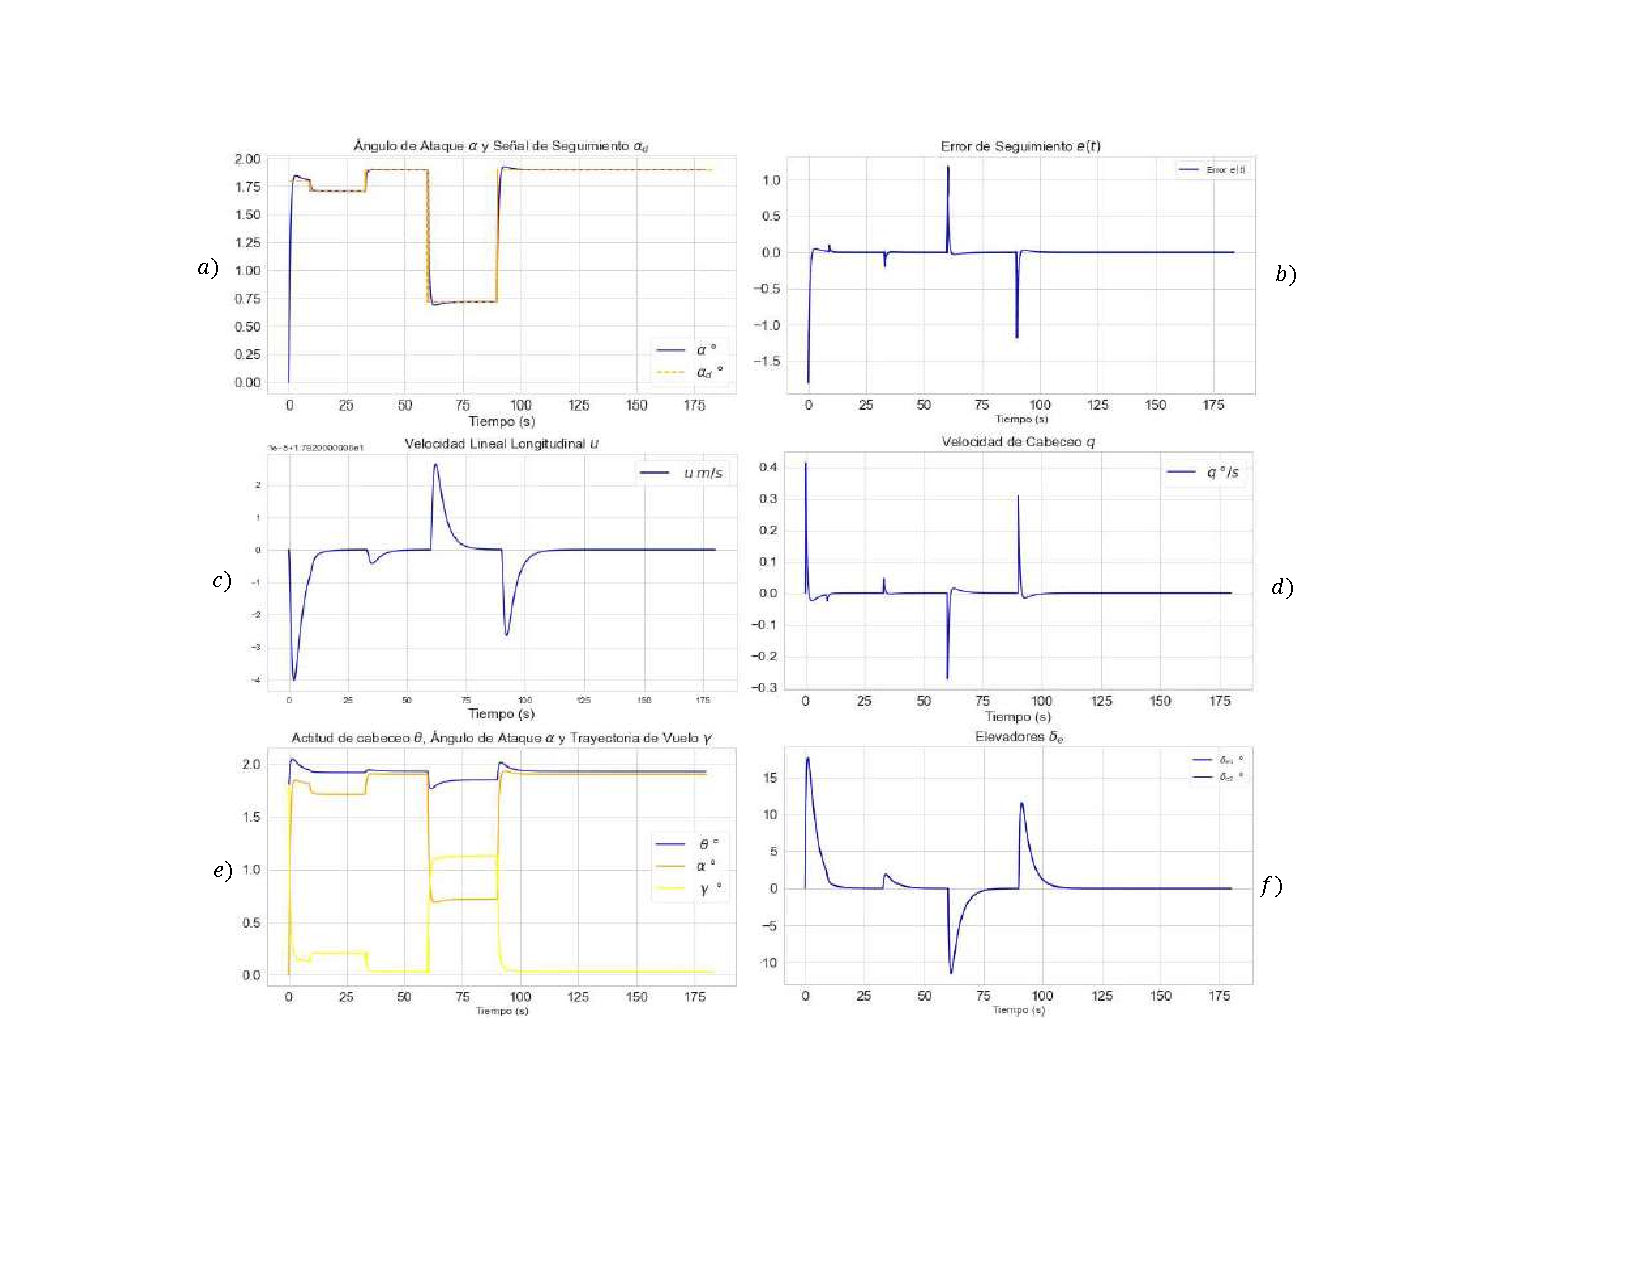
\includegraphics[scale=0.73]{Capitulo3/figs/Simulacion Backstepping Longitudinal 2_cropped.pdf}
    \caption{EHEKATL BWB Longitudinal Backstepping Simulation}
    \label{Simulación Backstepping Longitudinal de EHEKATL BWB}
\end{figure}

\begin{figure}[!h]
\centering
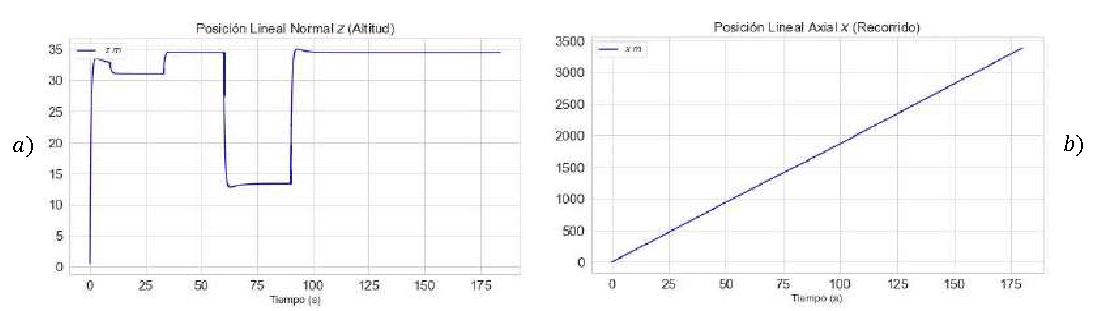
\includegraphics[scale=0.75]{Capitulo3/figs/Altitud y Recorrido Backstepping Longitudinal 2.pdf}
\caption{Simulation Backstepping Longitudinal - Altitude and Tour}
\label{Simulación Backstepping Altitud y Recorrido EHEKATL BWB}
\end{figure}

\textbf{Discussion of the Results:}
\begin{itemize}
    \item At the beginning of the simulation it is observed in graph a) that the desired path for the angle of attack $\alpha_d$ It's a little below the angle of attack in balance. $\alpha_e$so the angle of the flight path $\gamma$ rises slightly from the local horizon, however, after the first twenty-seven seconds $\gamma$ approaches zero (or horizon) since $\alpha_d$ approaches $\alpha_e$. The above describes a cruise flight, a straight and level flight. It is important to remember that the angle of pitch attitude and flight path are positive in the opposite direction of the handles with respect to the local horizon plane. However, the angle of attack is positive in the direction of the handles and from the body plane of EHEKATL BWB. Therefore, the results make sense and physical coherence.
    \item When $\alpha$ descends to $0.72$ the angle of the flight path is directed somewhat upwards, by the physical sense that we explained in the preceding paragraphs.
    \item In graph (c) the physical sense of linear velocity $u$ also has consistency. When the aircraft is heading upwards $u$ descends, and when the aircraft goes nose down speed $u$ This is due to the fact that every time the aircraft speed vector approaches the gravity velocity vector, the aircraft will gain speed at $u$. As the opposite happens, and from our flight reference (local axis horizon) $x$), each time the nose angle up increases the air resistance will be greater and the angle between the direction of the aircraft speed vector and the gravity vector also increases, so it decreases the speed of $u$. However, the aerodynamic parameters obtained in order of speed $u$ do not represent a significant magnitude in the simulations shown in \ref{Simulación Backstepping Longitudinal de EHEKATL BWB} Since it is worth it is very small. 
    \item In graph (d) the angular pitching speed $q$ It also has a physical sense by being positive when the pitching attitude is positive, and by being negative when the pitching attitude decreases. 
    \item In graph f) the response signal of the elevators  $\delta_{e1}$ $\delta_{e2}$ have practically the same deflection, which oscillates between the $15$ and $-10$ The elevators have a positive direction in the direction of the handles, i.e. when in response the aircraft's nose goes up. By deduction, when the elevators have a negative value the moment makes the aircraft go nose down.
    \item In \ref{Simulación Backstepping Altitud y Recorrido EHEKATL BWB} the kinematics is observed in the plane $x-z$. According to the variations in the angle of attack, in graph a) the aircraft oscillates at an altitude between $30-35m$ in the first 55 seconds, then descends to the $14m$ about, and goes back up to the $35m$ to maintain a constant altitude. In graph b) variations of $u$ are so small that they are indescribable in the linear position $x$, therefore, is observed with a fully linear slope. 
\end{itemize}

\medskip

\textbf{Lateral-Directional Backstepping Controller}\\
The three-degree lateral-directional dynamic model of freedom is now implemented in the structure \ref{estructura backstepping 1} for their representation in state space.
\begin{equation}
    \begin{bmatrix}
        \dot \beta \\
        \dot \phi
    \end{bmatrix}
    =
    \begin{bmatrix}
        \frac{1}{mV} (Y_\beta \beta + Y_p p + Y_r r + T C_\theta) - \frac{g}{V} S_\theta \\
        p
    \end{bmatrix}
    +
    \begin{bmatrix}
    w_e & - u_e \\
    0 & 0
    \end{bmatrix}
    \begin{bmatrix}
      p  \\
      r
    \end{bmatrix}
    +
    \begin{bmatrix}
     \frac{1}{mV} Y_{\delta_a} & \frac{1}{mV} Y_{\delta_r} \\
      0 & 0 \\
    \end{bmatrix}
    \begin{bmatrix}
        \delta_{a} \\
        \delta_{r} \\
    \end{bmatrix} \nonumber\\
\end{equation}

\begin{equation}
    \begin{bmatrix}
        \dot p \\
        \dot r
    \end{bmatrix}
    =
    \begin{bmatrix}
        \frac{1}{x} (L_\beta \beta + L_p p + L_r r) \\
        \frac{1}{z} (N_\beta \beta + N_p p + N_r r) \\
    \end{bmatrix}
    +
    \begin{bmatrix}
      \frac{1}{x} L_{\delta_{a}} &  \frac{1}{x} L_{\delta_{r}} \\
      \frac{1}{z} N_{\delta_{a}} & \frac{1}{z} N_{\delta_{r}} \\
    \end{bmatrix}
    \begin{bmatrix}
        \delta_{a} \\
        \delta_{r} \\
    \end{bmatrix}
\end{equation}

A-dimensional lateral aerodynamic coefficients for EHEKATL BWB were obtained with XFLR5 and are shown in the Table below. \ref{Coeficientes adimensionales laterales de EHEKATL BWB}. 
\begin{table}[!h]
    \centering
    \begin{tabular}{|cc|cc|cc|}
    \hline
     $C_{Y_\beta}$ & -0.30066 & $C_{Y_p}$ & -0.0422 & $C_{Y_r}$ & -0.193 \\
     \hline
     $C_{l_\beta}$ & -0.046761 & $C_{l_p}$ & -0.24566 & $C_{l_r}$ & 0.0343 \\
     \hline
     $C_{n_\beta}$ & 0.0848 & $C_{n_p}$ & -0.006445 & $C_{n_r}$ & -0.054 \\
     \hline
     $C_{Y_{\delta_a}}$ & 0.018585 & $C_{l_{\delta_a}}$ & 0.11009 & $C_{r_{\delta_a}}$ & 0.0032415 \\
     \hline
     $C_{Y_{\delta_r}}$ & 0.0228 & $C_{l_{\delta_r}}$ & 0.0406 & $C_{r_{\delta_r}}$ & -0.04523 \\
     \hline
    \end{tabular}
    \caption{A-dimensional lateral-directional coefficients of EHEKATL BWB}
    \label{Coeficientes adimensionales laterales de EHEKATL BWB}
\end{table}

According to the a-dimensional parameters obtained, using the formulas for the dimensional parameters of \ref{tab:derivadas dimensionales laterales} the results of the Table were obtained \ref{Coeficientes dimensionales laterales de EHEKATL BWB}.

\begin{table}[!h]
    \centering
    \begin{tabular}{|cc|cc|cc|}
    \hline
     ${Y_\beta}$ & -0.30066 & ${Y_p}$ & -0.0422 & ${Y_r}$ & -0.193 \\
     \hline
     ${L_\beta}$ & -0.046761 & ${L_p}$ & -0.24566 & ${L_r}$ & 0.0343 \\
     \hline
     ${N_\beta}$ & 0.0848 & ${N_p}$ & -0.006445 & ${N_r}$ & -0.054 \\
     \hline
     ${Y_{\delta_a}}$ & 0.018585 & ${L_{\delta_a}}$ & 0.11009 & ${N_{\delta_a}}$ & 0.0032415 \\
     \hline
     ${Y_{\delta_r}}$ & 0.0228 & ${L_{\delta_r}}$ & 0.0406 & ${N_{\delta_r}}$ & -0.04523 \\
     \hline
    \end{tabular}
    \caption{Side-way dimensional coefficients of EHEKATL BWB}
    \label{Coeficientes dimensionales laterales de EHEKATL BWB}
\end{table}

The reference signal can be both to command the sideslip angle and the roll angle. The simulations of the Figure \ref{Simulación Backstepping Lateral-Direccional de EHEKATL BWB} show the response of the lateral-directional dynamics with a Backstepping controller capable of commanding tracking signals according to a desired sideslip angle and/or wing angle. 

The tuned gains for the side-directional Backstepping controller are shown in \ref{ganancias backstepping lateral-direccional}. 

\begin{equation}
\label{ganancias backstepping lateral-direccional}
    k_\beta = 0.9603, k_\phi = 0.0993, k_p = 0.03, k_r = 0.3, k_{\delta_a} = 0.9, k_{\delta_r} = 0.9
\end{equation}

\begin{figure}[!h]
    \centering
    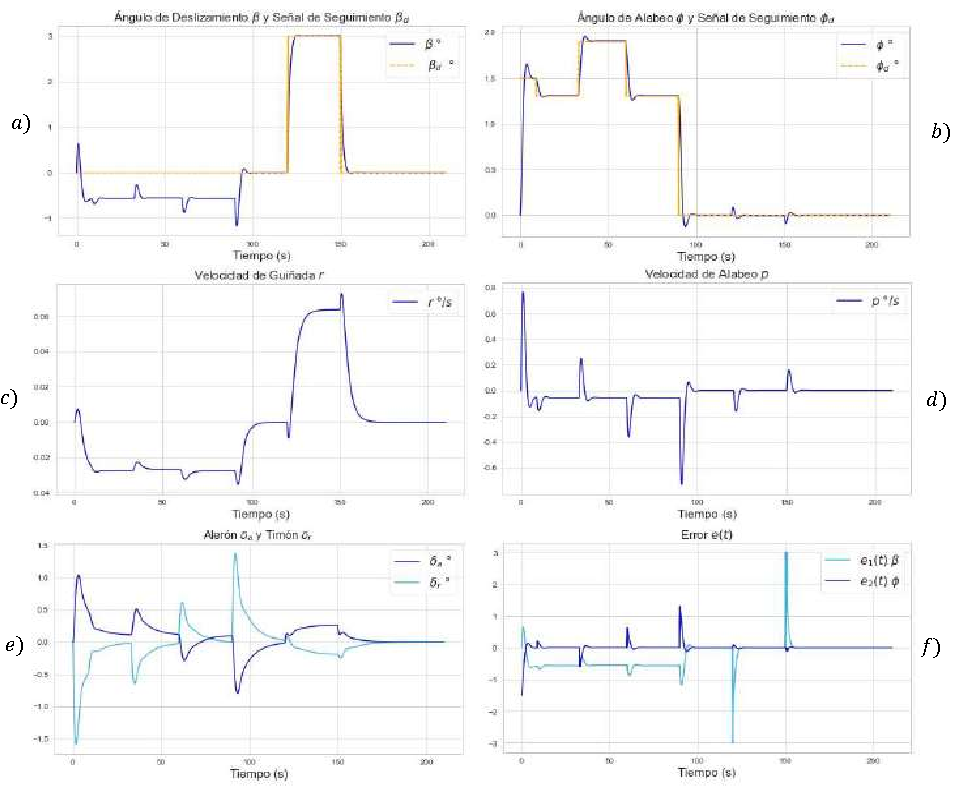
\includegraphics[scale=0.87]{Capitulo3/figs/Simulacion Backstepping LateralDireccional 2.pdf}
    \caption{EHEKATL BWB Lateral-Directional Backstepping Simulation}
    \label{Simulación Backstepping Lateral-Direccional de EHEKATL BWB}
\end{figure}

\begin{figure}[!h]
    \centering
    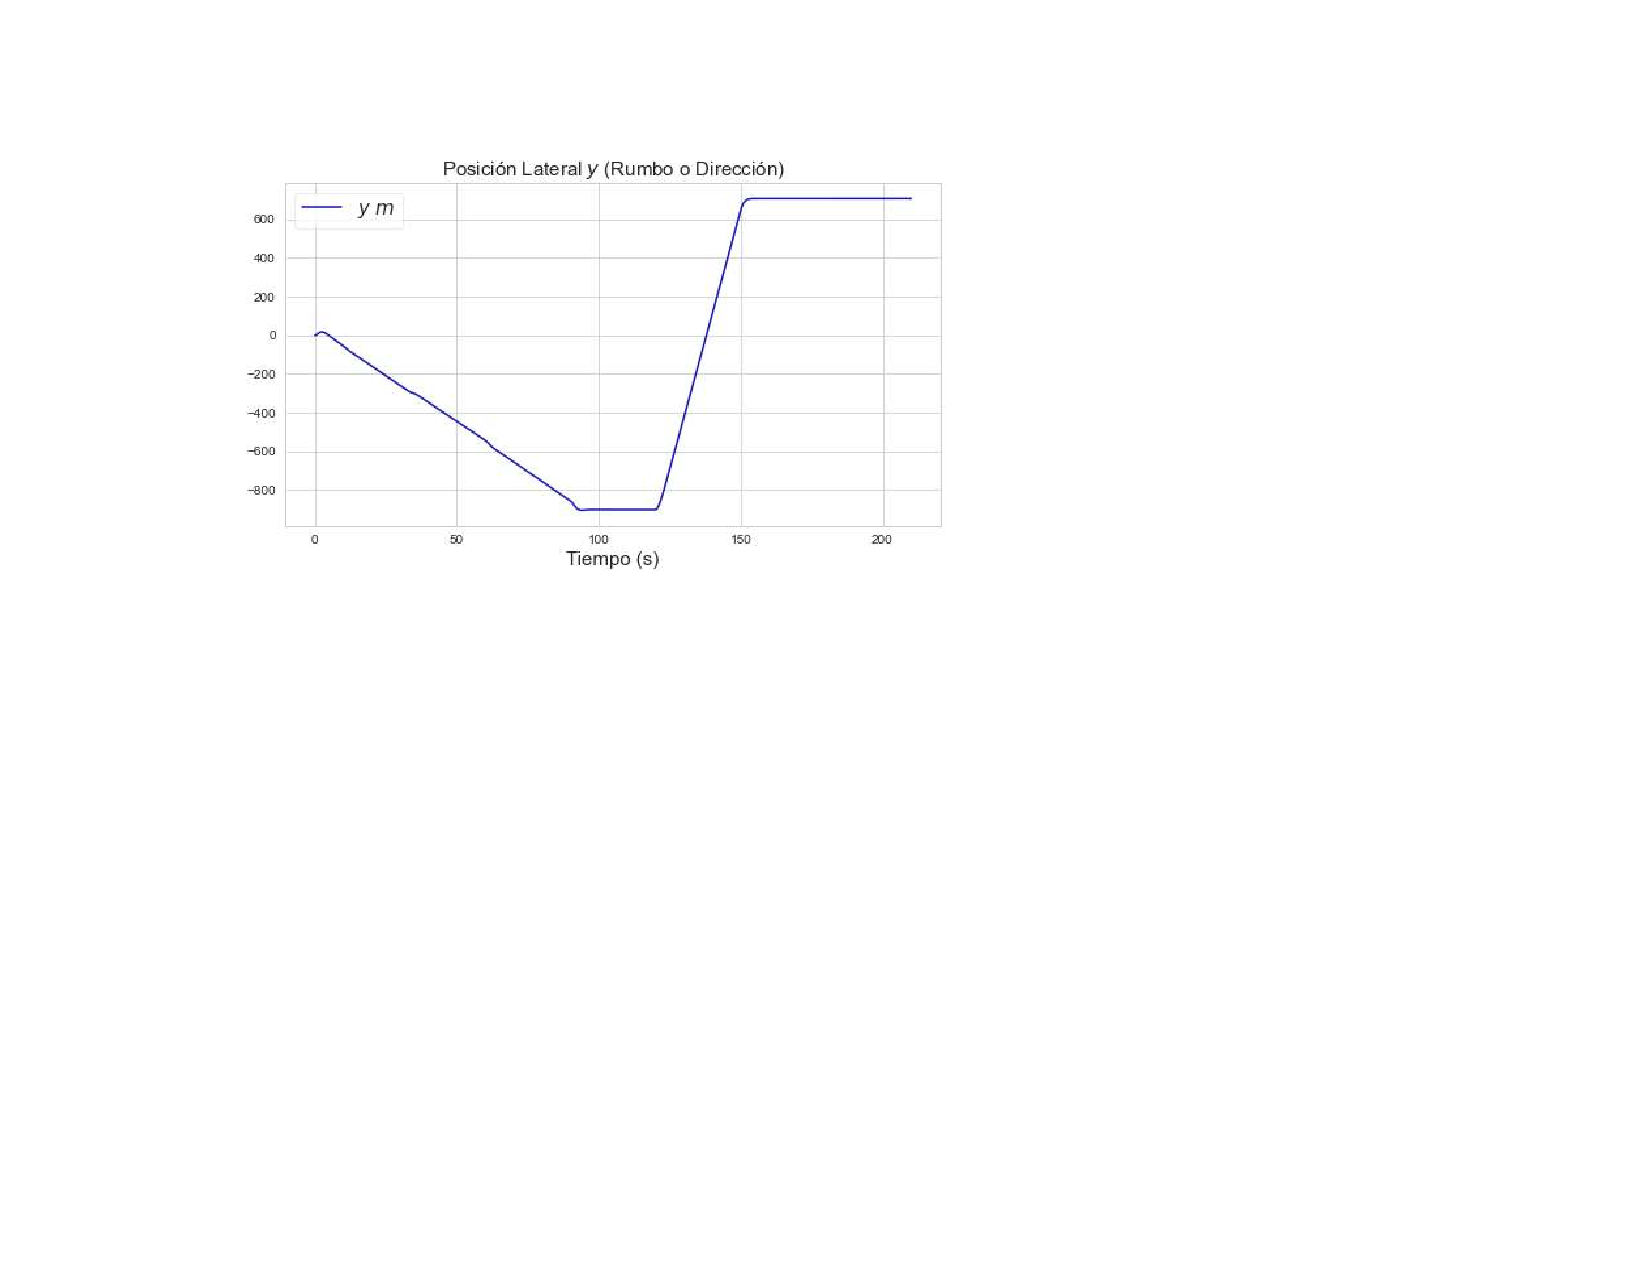
\includegraphics[scale=0.9]{Capitulo3/figs/Simulacion Backstepping LateralDireccional RumboDireccion_cropped.pdf}
    \caption{EHEKATL BWB Lateral-Directional Backstepping Simulation: Side Position $y$ (rombo or address)}
    \label{Simulación Backstepping Lateral-Direccional de EHEKATL BWB: Posición lateral y (rumbo o dirección)}
\end{figure}

\textbf{Discussion of the Results:}
\begin{itemize}
    \item In the simulation \ref{Simulación Backstepping Lateral-Direccional de EHEKATL BWB} is shown in graphs (a) and (b) the tracking of both angles, $\beta$ and $\phi$, respectively; fundamental in lateral-directional dynamics. First, it commands for EHEKATL BWB a tracking signal for the wing angle, where through a step type signal it was maintained in an roll of between 1.3$^\circ$ - 1.9$^\circ$In the first 90 seconds.
    \item For the second one hundred and twenty, a sideslip angle of 3 is commanded.$^\circ$ for thirty seconds, to return to a straight and level flight with $\beta=0$ and $\phi=0$ and finish the simulation.
    \item It is observed that the generation of a wing angle $\phi$ has an answer at the sideslip angle $\beta$, who defines the orientation of the speed vector of EHEKATL BWB. Hopefully, in graph (c) the yaw speed has a direct relation to the sideslip angle, while in graph (d) the wing speed $p$ with the wing angle proper. 
    \item In graph (e) the response of the wings is in the range of 1$^\circ$ a -1$^\circ$, while the rudder response is 1.5$^\circ$ a -1.5$^\circ$.
    \item In graph f) the error of $\beta$ is kept out of follow-up during the tracking of the wing signal, and with all physical consistency, since the wing angle generates this response at the sideslip angle, and therefore this error is to be expected. The error behavior is very fast in approaching the track signal, and given the complexity of the nonlinearities and the coupling of the lateral-directional dynamics is considered the tuning of the gains of the Lateral-Directional Backstepping controller as satisfactory. 
    \item Finally, the Figure \ref{Simulación Backstepping Lateral-Direccional de EHEKATL BWB: Posición lateral y (rumbo o dirección)} shows the side position $y$, which in aeronautics is known as direction or direction, and given the speed of $17.82 m/s$ provides such results. The negative and positive sense of $y$ coincides with the sense of $\beta$. 
\end{itemize}


%%%%%%%%%%%%%%%%%%%%%%%%%%%%%%%%%%%%%%%%%%%%
\section{Adaptive Backstepping}

The term Adaptable, as far as control is concerned, has the quality of adjusting parameters and/or control actions in order to deal with changes, uncertainties or variations in the dynamic system. In aircraft dynamics, aerodynamic coefficients are complex to obtain accurately, and uncertainties and variations can occur over time due to factors such as external disturbances, changes in system parameters and environmental conditions. 

%Los principios básicos del diseño del controlador \textit{Adaptive Backstepping} de EHEKATL BWB envuelven tres componentes esenciales:
%\begin{itemize}
    %\item \textbf{Identificación del Sistema.} Vamos a considerar $f_1$ y $f_2$, funciones que describen las fuerzas y momentos aplicados en EHEKATL BWB como parámetros desconocidos.  
    %\item \textbf{Leyes de Adaptación.} De acuerdo con la identificación de $f_1$ $f_2$ las leyes de adaptación se diseñan para actualizar los parámetros del controlador. Las leyes de adaptación utilizan parámetros de estimación y el estado actual de las variables de estado del sistema para determinar cuanto ajustar las acciones de control de $\delta_e$ $\delta_a$ $\delta_r$
    %\item \textbf{Leyes de Control.} Las leyes de control son la pieza principal del controlador adaptable dado que generan las acciones de control de acuerdo con las variables de estado del sistema y los parámetros de adaptación. Combinan el proceso de adaptación con el objetivo de control (señal de seguimiento o comando de referencia), logrando la estabilidad del sistema y el desempeño deseado.
%\end{itemize}

The implementation of an adaptive controller is suitable for EHEKATL BWB given the complex dynamics of the system where accurate knowledge of system dynamics can be a challenge, in addition to the changes they experience during flight operation. 

\medskip

\textbf{Adaptive Backstepping Controller}\\
The non-linear dynamics of EHEKATL BWB are represented in the same structure used for the Bacsktepping controller. 

\begin{align}
    \dot x_{1} &= f_{1} + g_1 x_2 + h_1 u \\ \nonumber
    \dot x_{2} &= f_{2} + g_2 u \\ \nonumber
\end{align}

Estimation errors are established $\Tilde{f_1}$ $\Tilde{f_2}$ for estimating values $\hat{f_1}$ $\hat{f_2}$ of unknown parameters $f_1$ $f_2$. 
\begin{gather}
    \Tilde{f_1} =f_1 - \hat{f_1}\\ \nonumber
    \Tilde{f_2} = f_2 - \hat{f_2} \nonumber
\end{gather}

where

$\hat{f_1}$ and $\hat{f_2}$ are the estimated values of $f_1$ and $f_2$.

$\Tilde{f_1}$ and $\Tilde{f_2}$ are the estimation errors of $f_1$ and $f_2$.


We defined three blocks of estimation errors: 1) $z_1, z_2$ for status variables with respect to follow-up signals, 2) $z_3$ for the command of the control entries $u$ with regard to the virtual control law $u^d$ and 3) $\Tilde{f_1}, \Tilde{f_2}$ concerning the functions with uncertainty of forces and moments of EHEKATL BWB $f_1, f_2$ with respect to its estimating functions $\hat{f_1}, \hat{f_2}$. 

\begin{align}
\label{errorres de estimacion adaptive}
    z_1 &= x_1 - x^d_1 \\ \nonumber
    z_2 &= x_2 - x^d_2 \\ \nonumber
    z_3 &= u - u^d \\ \nonumber
    \Tilde{f_1} &= f_1 - \hat{f_1} \\ \nonumber
    \Tilde{f_2} &= f_2 - \hat{f_2} \\ \nonumber
\end{align}

The error $z_3$ It derives from our consideration of the dynamics of the actuators, where we consider a delay of first order. $u$ real considered in the dynamics of the actuators is produced by the following process. We will define the function of transfer of the dynamics of the actuators: 

\begin{equation}
    \dot u = - \frac{1}{\tau}u + \frac{1}{\tau} u_c
\end{equation}

where:

$\tau:$ \textit{tiempo constante}


$u_{c}:$ \textit{control command generated by the controller} 


$u:$ \textit{real dynamic command of actuators}


We propose a Lyapunov candidate function for each of the estimation errors defined in \ref{errorres de estimacion adaptive}. 
\begin{equation}
    V_1 (z_1, z_2, z_3, \Tilde{f_1}, \Tilde{f_2}) = \frac{1}{2} z_1^T z_1 + \frac{1}{2} z_2^T z_2 + \frac{1}{2} z_3^T z_3 + \frac{1}{2} \Tilde{f_1^T} \Gamma_1 \Tilde{f_1} + \frac{1}{2} \Tilde{f_2^T} \Gamma_2 \Tilde{f_2}
\label{lyapunov 2}
\end{equation}

For estimation errors $z_1, z_2,z_3$ We're going to propose virtual control laws that offset the terms of the equation and also contain the term of the controller. $k_n, z_n$. for estimation errors $ \Tilde{f_1}, \Tilde{f_2}$ We are going to propose adaptation laws that compensate the terms through parameters with estimation gains. 

First, we derive Lyapunov's proposed candidate role from \ref{lyapunov 2}. 
\begin{align}
       \dot V &= z^T_1 \dot z_1 + z^T_2 \dot z_2 + z^T_3 \dot z_3 + \Tilde{f_1^T}  \Gamma_1 \dot{\Tilde{f_1}} + \Tilde{f_2^T} \Gamma_2 \dot{\Tilde{f_2}} \nonumber \\
        &= z^T_1 (\dot x_1 - \dot x^d_1) + z^T_2 (\dot x_2 - \dot x^d_2) + z^T_3 (\dot u - \dot u^d) + \Tilde{f_1^T}  \Gamma_1 \dot{\Tilde{f_1}} + \Tilde{f_2^T} \Gamma_2 \dot{\Tilde{f_2}} \nonumber \\ 
    &= z^T_1 (f_1 + g_{1} x_2 - \dot x^d_1) + z^T_2 (f_2 + g_{2} u - \dot x^d_2) + z^T_3 (\frac{1}{\tau}(u_c - u) - \dot u^d) + \Tilde{f_1^T}  \Gamma_1 \dot{\Tilde{f_1}} + \Tilde{f_2^T} \Gamma_2 \dot{\Tilde{f_2}} \nonumber \\
    &= z^T_1 (f_1 + g_{1} (z_2 + x_{2}^d)  + h_1 z_3 + h_1 u - \dot x^d_1) + z^T_2 (f_2 + g_{2} (z_3 + u^d) - \dot x^d_2)  \nonumber \\
    &+ z^T_3 (\frac{1}{\tau}(u_c - u) - \dot u^d) + \Tilde{f_1^T}  \Gamma_1 \dot{\Tilde{f_1}} + \Tilde{f_2^T} \Gamma_2 \dot{\Tilde{f_2}}
\end{align}


According to the previous development, we propose the following virtual control laws. 

\begin{align}
    x^d_2 &= \frac{1}{g_{1}} [- \hat{f_1^T} + \dot x^d_1 - k_1 z_1] \nonumber \\
    u^d &= \frac{1}{g_{2}} [- \hat{f_2^T} + \dot x_{2}^d - k_2 z_2 - g_{1}^T z_1] \nonumber \\
    u_c &= u + \tau [\dot u^d - g_{2}^T z_2 - (h_1^Tu + h_1^T)z_1 - k_3 z_3]
\end{align}

We replace and continue development.  

\begin{align}
      \dot V &=  z^T_1 (f_1 + g_{1} (z_2 + [\frac{1}{g_{1}} [- \hat{f_1^T}  + \dot x^d_1 - k_1 z_1]]) + h_1 z_3 + h_1 u - \dot x^d_1) \nonumber \\
      &+ z^T_2 (f_2 + g_{2} (z_3 + [\frac{1}{g_{2}} [- \hat{f_2^T} + \dot x_{2}^d - k_2 z_2 - g_{1}^T z_1]]) - \dot x^d_2) \nonumber \\
      &+ z^T_3 (\frac{1}{\tau}([ u + \tau [\dot u^d - g_{2}^T z_2 - u h_1^T z_1 - h_{1}^T z_1 - k_3 z_3]] - u) - \dot u^d) \nonumber \\
      &+ \Tilde{f_1^T}  \Gamma_1 \dot{\Tilde{f_1}} + \Tilde{f_2^T} \Gamma_2 \dot{\Tilde{f_2}} \nonumber \\
      &= z^T_1 (\Tilde{f_1} + g_1 z_2  + h_1 z_3 + h_1 u - k_1 z_1) + z^T_2 (\Tilde{f_2} \nonumber \\
      &+ g_2 z_3 - g^T_1 z_1 - k_2 z_2) + z^T_3 (- u h_1^T z_1 - h_1^T z_1  - g_{2}^T - k_3 z_3) \nonumber \\
      &+ \Tilde{f_1^T}  \Gamma_1 \dot{\Tilde{f_1}} + \Tilde{f_2^T} \Gamma_2 \dot{\Tilde{f_2}} \nonumber \\
      &= z^T_1 \Tilde{f_1} + (z^T_1g_1 z_2 - z^T_2 g^T_1 z_1 ) + (z_1^T(h_1 (z_3 + u)) - h_1^T(z_1(1+u))) - z^T_1 k_1 z_1 + z^T_2 \Tilde{f_2} \nonumber \\ 
      &+ (z^T_2 g_2 z_3 - z^T_3 g_{2}^T z_2 ) -  z^T_2 k_2 z_2 - z^T_3  k_3 z_3 + \Tilde{f_1^T}  \Gamma_1 \dot{\Tilde{f_1}} + \Tilde{f_2^T} \Gamma_2 \dot{\Tilde{f_2}} \nonumber \\
      &= z^T_1 \Tilde{f_1} + z^T_2 \Tilde{f_2} - z^T_1 k_1 z_1 - z^T_2 k_2 z_2 -  z^T_3  k_3 z_3  + \Tilde{f_1^T}  \Gamma_1 \dot{\Tilde{f_1}} + \Tilde{f_2^T} \Gamma_2 \dot{\Tilde{f_2}}
\end{align}

We can appreciate the terms $\Tilde{f_1^T}  \Gamma_1 \dot{\Tilde{f_1}} ,  \Tilde{f_2^T} \Gamma_2 \dot{\Tilde{f_2}}$. We will compensate them by proposing the following adaptation laws. 

\begin{gather}
    \dot{\Tilde{f_1}} = \dot f_1 - \dot{\hat{f_1}} = - \Gamma_{1}^{-1} z_1 \\ \nonumber
    \dot{\Tilde{f_2}} = \dot f_2 - \dot{\hat{f_2}} = - \Gamma_{2}^{-1} z_2 \nonumber
\end{gather}

By replacing the adaptation laws, we finished the development of the derivative of Lyapunov's candidate function.  

\begin{align}
      \dot V &= z^T_1 \Tilde{f_1} + z^T_2 \Tilde{f_2} - z^T_1 k_1 z_1 - z^T_2 k_2 z_2 -  z^T_3  k_3 z_3  + \Tilde{f_1^T}  \Gamma_1 (- \Gamma_{1}^{-1} z_1) + \Tilde{f_2^T} \Gamma_2 (- \Gamma_{2}^{-1} z_2) \nonumber \\ 
      &= z^T_1 \Tilde{f_1} + z^T_2 \Tilde{f_2} - z^T_1 k_1 z_1 - z^T_2 k_2 z_2 -  z^T_3  k_3 z_3  - \Tilde{f_1^T} z_1 - \Tilde{f_2^T} z_2 \nonumber \\
      &= - z^T_1 k_1 z_1 - z^T_2 k_2 z_2 -  z^T_3  k_3 z_3
\end{align}

\begin{equation}
\label{adapt lya yeah}
    \dot V = - z^T_1 k_1 z_1 - z^T_2 k_2 z_2 -  z^T_3  k_3 z_3 \\
\end{equation}

And therefore:
\begin{equation}
    \dot V \leqslant 0
\end{equation}

According to the La Salle-Yoshizawa theorem, the states $z_1,z_2,z_3$ converge asymptotically to the origin as  $t\to\infty$This is it, $z_1=z_2 = z_3 \to 0$ which implies that $x_1\to x_1^d$, $x_2\to x_2^d$ and $u\to u^d$. In addition with the equation \ref{adapt lya yeah} We have to $z_1, z_2, z_3 \in L_2$. 

\medskip

\textbf{Adaptive Backstepping Controller Longitudinal}\\
For the design of the EHEKATL BWB Longitudinal Adaptive Backstepping controller, the promotion regimen tracking signal, known as $ROC$. In the Longitudinal Backstepping controller we command the attack angle signal considering the dynamic model with wind shafts, now we command the normal linear velocity $w$ sinonima to $ROC$ considering the dynamic model in the body axes. The difference between one application and another is the use of reference systems.

The structure representing states according to the nonlinear longitudinal dynamics of EHEKATL BWB is represented as follows. 

\begin{equation}
    \begin{bmatrix}
        \dot u \\
        \dot w
    \end{bmatrix}
    =
    \begin{bmatrix}
        \frac{1}{m} (X_u u + X_w w + X_q q + T C_\theta) - \frac{g}{V} S_\theta \\
        \frac{1}{m} (Z_u u + Z_w w + Z_q q + T S_\theta) + \frac{g}{V} C_\theta
    \end{bmatrix}
    +
    \begin{bmatrix}
    - w & 0 \\
    u & 0
    \end{bmatrix}
    \begin{bmatrix}
      q  \\
      \theta
    \end{bmatrix}
    +
    \begin{bmatrix}
     \frac{1}{m} X_{\delta_e1} & \frac{1}{m} X_{\delta_e2} \\
     \frac{1}{m} Z_{\delta_e1} & \frac{1}{m} Z_{\delta_e2} \\
    \end{bmatrix}
    \begin{bmatrix}
        \delta_{e1} \\
        \delta_{e2} \\
    \end{bmatrix} \nonumber\\
\end{equation}

\begin{equation}
    \begin{bmatrix}
        \dot q \\
        \dot \theta
    \end{bmatrix}
    =
    \begin{bmatrix}
        \frac{1}{y} (M_u u + M_w w + M_q q) \\
        q \\
    \end{bmatrix}
    +
    \begin{bmatrix}
     \frac{1}{I_y} M_{\delta_{e1}} & \frac{1}{I_y} M_{\delta_{e2}} \\
      0 & 0 \\
    \end{bmatrix}
    \begin{bmatrix}
        \delta_{e1} \\
        \delta_{e2} \\
    \end{bmatrix}
\end{equation}

According to the aerodynamic simulations with XFLR5 we obtained the dimensional parameters of EHEKATL BWB. 

\begin{table}[!h]
    \centering
    \begin{tabular}{|cc|cc|cc|}
    \hline
     $X_u$ & -0.027843 & $X_w$ & 0.34641 & $X_q$ & 0.0 \\
     \hline
     $Z_u$ & -1.5092 & $Z_w$ & -17.434 & $Z_q$ & -5.415 \\
     \hline
     $M_u$ & 6.1021e-07 & $M_w$ & -2.5615 & $M_q$ & -1.1697 \\
     \hline
     $X_{\delta_{e1}}$ & 0.30605 & $Z_{\delta_{e1}}$ &-8.8438 & $M_{\delta_{e1}}$ & -2.3445 \\
     \hline
     $X_{\delta_{e2}}$ & 0.30605 & $Z_{\delta_{e2}}$ & -8.8438 & $M_{\delta_{e2}}$ & -2.3445 \\
     \hline
    \end{tabular}
    \caption{Longitudinal dimensional coefficients of EHEKATL BWB 2}
    \label{Coeficientes dimensionales longitudinales de EHEKATL BWB adaptive}
\end{table}

The objective of the simulation of the Figure \ref{Simulación para la dinámica longitudinal de EHEKATL BWB con el controlador Adaptive Backstepping} is commanding ROC to manage to ascend and descend to EHEKATL BWB. 

According to the results of \ref{Coeficientes dimensionales longitudinales de EHEKATL BWB adaptive} a constant speed of $V_T = 17 m/s$ with an angle of attitude in balance of $\theta_e = 1.8$. 

Gains from virtual control laws and adaptation laws are shown in \ref{ganancias adaptive backstepping longitudinal}.
\begin{align}
\label{ganancias adaptive backstepping longitudinal}
    k_u = 1.5, k_w = 1.5, k_q = 1.5, k_\theta = 0.3 \\ \nonumber
    k_{\delta_{e_u}} = 120, k_{\delta_{e_w}} = 120, k_{\delta_{e_q}} = 120, k_{\delta_{e_\theta}} = 60 \\ \nonumber
    \Gamma_u = 12, \Gamma_w = 15, \Gamma_q = 15, \Gamma_\theta = 9 \nonumber
\end{align}


\begin{figure}[!t]
    \centering
    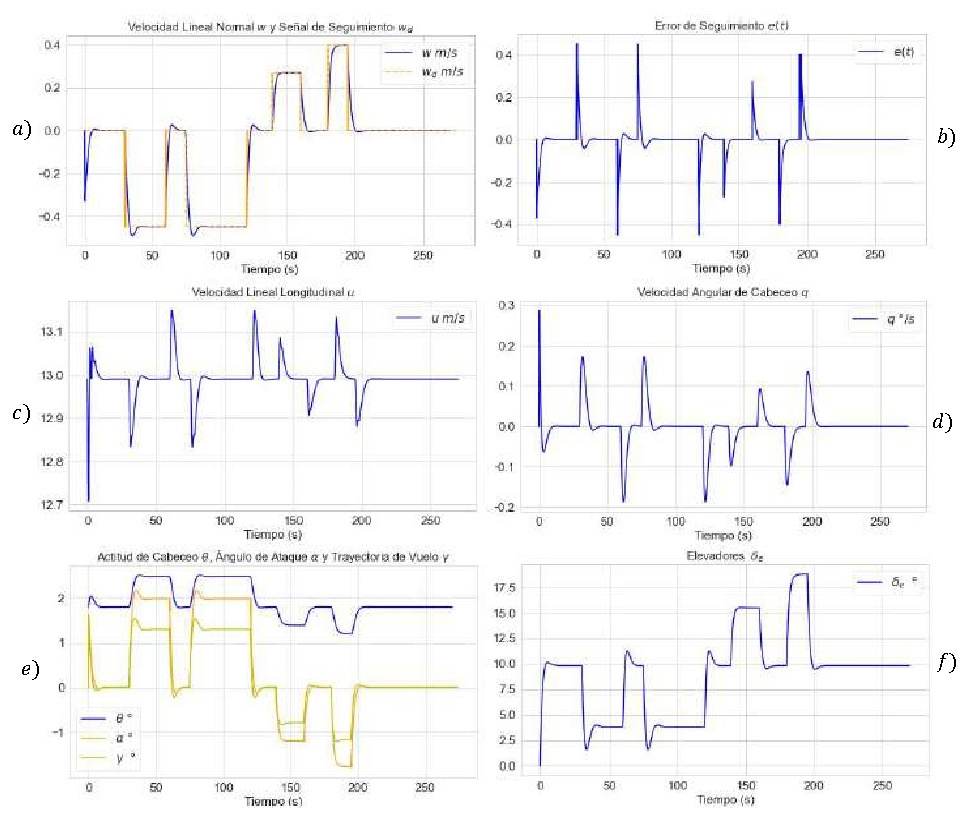
\includegraphics[scale=0.86]{Capitulo3/figs/Simulacion Adaptive Backstepping Longitudinal 2.pdf}
    \caption{Simulation for the longitudinal dynamics of EHEKATL BWB with the Adaptive Backstepping controller}
    \label{Simulación para la dinámica longitudinal de EHEKATL BWB con el controlador Adaptive Backstepping}
\end{figure}

\textbf{Discussion of Results:}
\begin{itemize}
    \item In graph (a) the tracking signal $w_d$ command the ascent regime for EHEKATL BWB. It is important to remember that the body axis $z$ is headed down, so the ascent is defined with $-w$, while the descent is defined with $+w$. 
    \item The simulation time is 270 seconds. $w_d$ is a step type signal with two ascents and two descents, ending at a constant altitude.
    \item The first row of the gains tune to the law of control of the dynamics of the aircraft, the gains of the second row tune the law of control of the dynamics of the actuators, finally, the gains of the third row tune the law of adaptation of the unknown parameters.
    \item In graph f) when the simulation starts the elevators have a deflection of $-10$ degrees, but just after it fits $0$ degrees where the flight is maintained at constant altitude. When the ascent regime begins (value of $w$ negative) the elevators do deflection with negative value, while the angle of attitude and angle of attack are positive, according to their frame of reference. 
    \item in graph (e) the flight path is defined as the difference between the pitching attitude and the angle of attack, then, in the first instant of the simulation the adjustment at the three angles is perceived according to the deflection of the elevators. Then the balance pitch attitude is maintained. $1.88$ for a flight at constant altitude. 
    \item When the first two steps of the angle of attack are generated, it is observed that it increases the pitch attitude but in a lesser reason and the flight path increases with a positive angle, in relation to the increase of altitude that is being obtained. 
    \item When a negative attack angle is generated at constant speed, it means that now the velocity vector is above the aircraft, and the angle of the flight path is also negative result at a descending altitude. 
    \item Finally, in the Figure \ref{Trayectoria para la dinámica longitudinal de EHEKATL BWB con el controlador Adaptive Backstepping} the position in the plane is observed $x-z$ of EHEKATL BWB according to the constant speed of $17 m/s$ and changes in the promotion regime $w$. According to the trajectory we can include the phases of take-off, ascent, cruise and descent. 
\end{itemize}

\begin{figure}[!t]
    \centering
    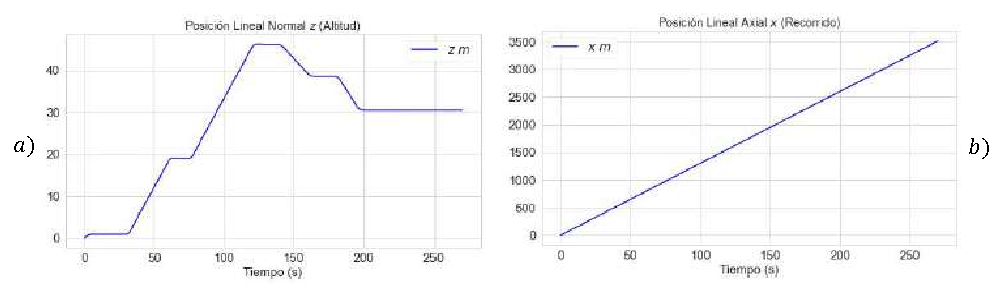
\includegraphics[scale=0.85]{Capitulo3/figs/Simulacion Adaptive Backstepping Longitudinal Posicion 2.pdf}
    \caption{Simulation Trajectory for the Longitudinal Dynamics of EHEKATL BWB with Adaptive Backstepping Controller}
    \label{Trayectoria para la dinámica longitudinal de EHEKATL BWB con el controlador Adaptive Backstepping}
\end{figure}

%%%%%%%%%%%%%%%%%%%%%%%%%%%%%%%
\section{Comparative Analysis}

When you have the design of various flight control systems you can perform a comparative analysis through \textbf{performance indicators} that evaluate the response of each FCS for different types of input in terms of stability, accuracy and robustness. 

The performance indicators to be used are as follows:
\begin{itemize}
    \item \textbf{ISE (Integration of quadratic error)} In aircraft control, ISE can be used to assess the performance of FCS according to how well it is to track the desired trajectory. Therefore, if the aircraft is following a specific flight path. 
    \item \textbf{ITSE (Integration of quadratic error by time)} It takes into account the magnitude of the error and the time it takes to converge the system. In aircraft control, the ITSE can evaluate the ability of the control system to respond quickly and minimize over-jumps. A low value of the ITSE corresponds to rapid and smooth changes in the desired flight condition. 
    \item  \textbf{ITAE (Integration of absolute error by time)} It is used in aircraft control because it minimizes absolute error while considering time. It is important in aviation where accuracy and its response over time are crucial. A small value in ITAE offers precision and speed in control response. 
    \item \textbf{IAE (Integration of absolute error)} It is a measure of how well the control system keeps the error within acceptable limits. In aircraft control, it is related to the stability and minimization of deviations according to a desired flight path. A lower value in IAE suggests a more stable and controllable aircraft during flight. 
\end{itemize}

In \ref{indices de desempeño}, the equations used for each performance index are shown. 
\begin{align}
\label{indices de desempeño}
    ISE = \int e^2  dt \\ \nonumber
    ITSE = \int t e^2 dt \\ \nonumber
    ITAE = \int t |e| dt \\ \nonumber
    IAE = \int |e| dt \\ \nonumber
\end{align}

%\begin{figure}[!h]
%    \centering
%    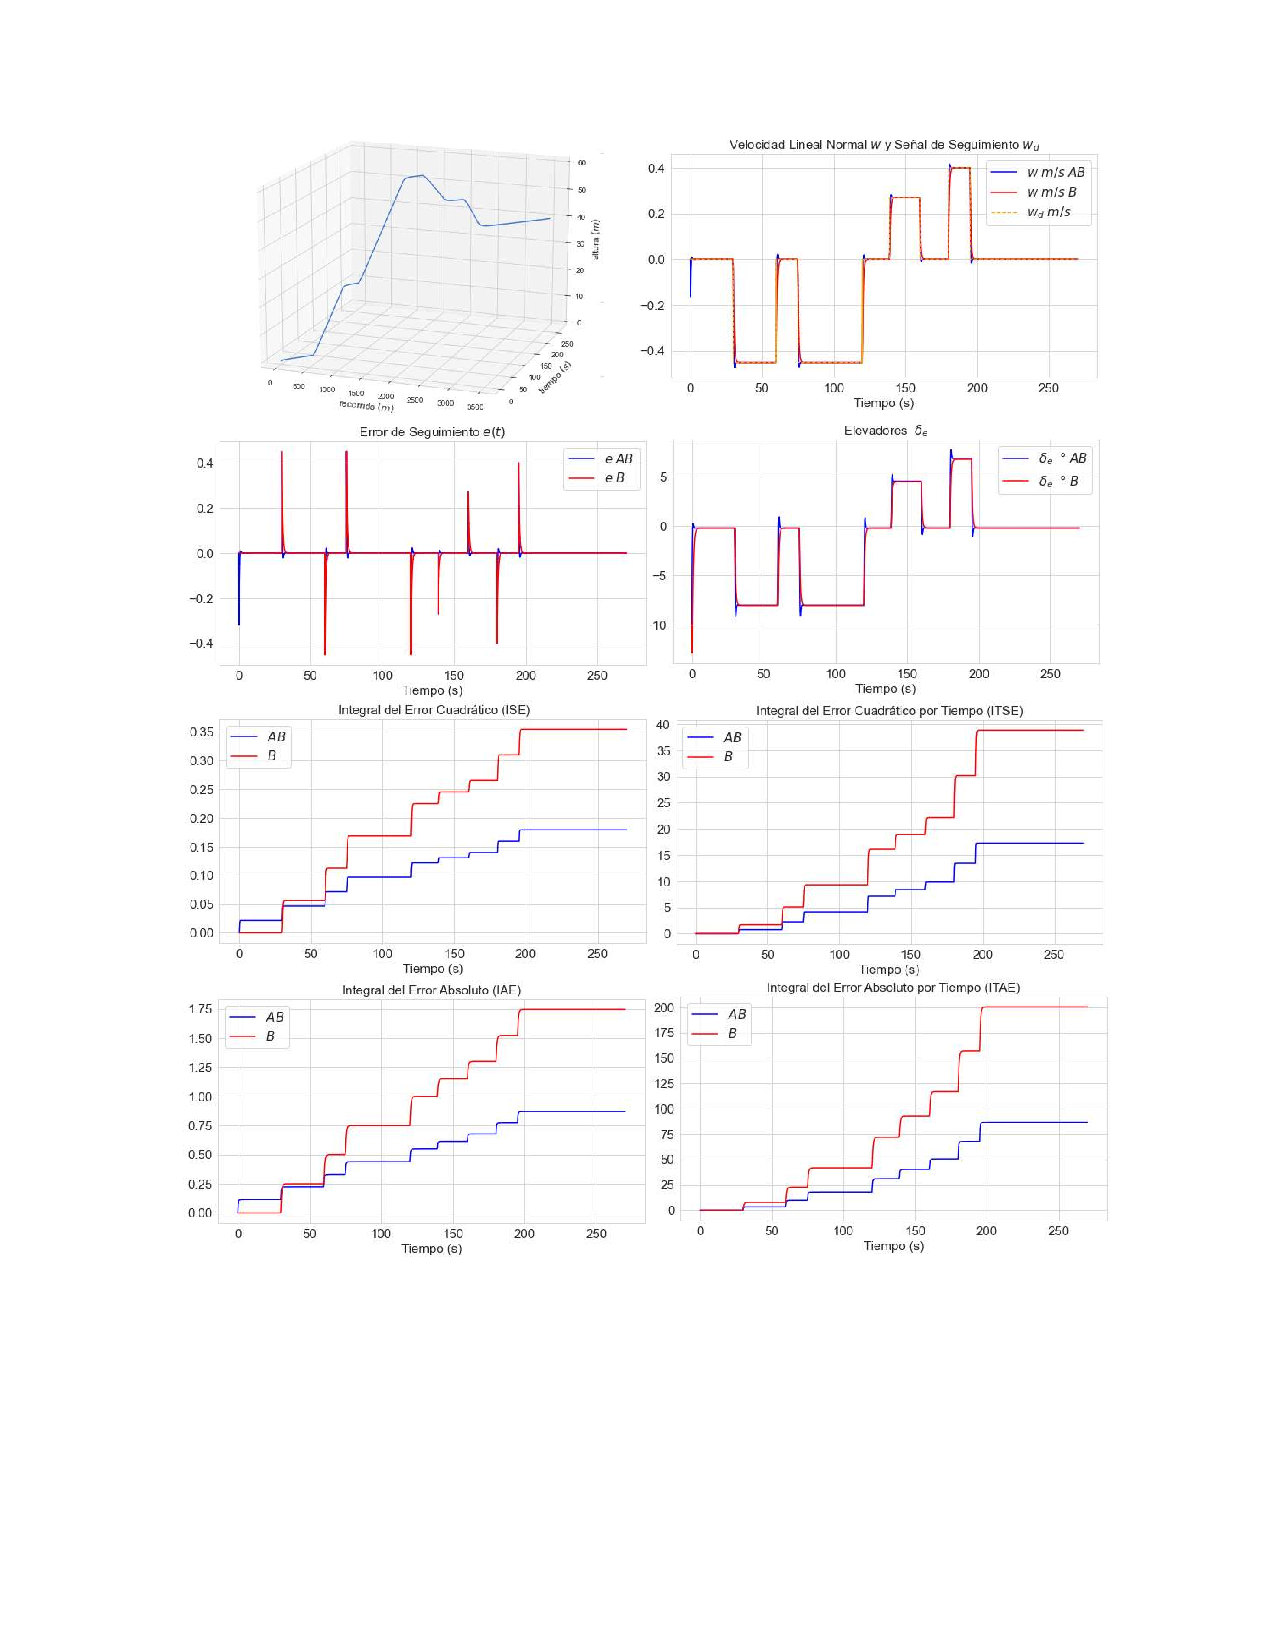
\includegraphics[scale=0.84]{Capitulo3/figs/Simulacion Analsis Comparativo_cropped.pdf}
%    \caption{Simulación - Análisis comparativo con indicadores de desempeño de controladores \textit{Adaptive Backstepping} y \textit{Backstepping} para la dinámica longitudinal de EHEKATL BWB}
%    \label{Simulacion Comparativa}
%\end{figure}
%En \ref{Simulacion Comparativa}, se aplicaron los índices de desempeño para evaluar los controladores Backstepping y Adaptive Backstepping de acuerdo a una trayectoria deseada en el régimen de ascenso en la dinámica longitudinal de EHEKATL BWB. 
%
The simulation that was carried out was identical to that carried out in \ref{Simulación para la dinámica longitudinal de EHEKATL BWB con el controlador Adaptive Backstepping}.

Performance index results in the evaluation of Backstepping drivers (\textit{B}) and Adaptive Backstepping (\textit{AB}) are shown numerically in the Table \ref{Indices de desempeño de controladores Backstepping y Adaptive Backstepping} and the following observations are made.

\begin{table}[!h]
    \caption{Backstepping and Adaptive Backstepping Driver Performance Indices}
    \centering
    \begin{tabular}{|c|c|c|c|c|}
    \hline
    \textbf{Control Strategy} & \textbf{ISE} & \textbf{ITSE} & \textbf{ITAE} & \textbf{IAE} \\
    \hline
    Backstepping  & 0.354388888 & 38.8511079 & 200.402469 & 1.74444444 \\
    Adaptive Backstepping & 0.17946439 & 17.2974672 & 86.7001543 & 0.87067341 \\
    \hline
    \end{tabular}
    \label{Indices de desempeño de controladores Backstepping y Adaptive Backstepping}
\end{table}


\bigskip

\textbf{Discussion of the results:}
\begin{itemize}
    \item In general, the controller \textit{AB} offers a better performance than \textit{B} according to the four performance indices. 
    %Puntualmente, los indicadores que no multiplican por el tiempo, \textit{ISE} y \textit{IAE}, muestran al principio de la simulación un error mayor de \textit{AB} únicamente antes de la primer transición de acuerdo con la señal de seguimiento $w_d$. Esto debido a que \textit{AB} muestra una ligera perturbación al inicio de la simulación, situación que no se presenta en \textit{B}. 
    %\item Los indicadores de desempeño que consideran y multiplican por el tiempo, \textit{ITSE} y \textit{ITAE}, no presentan esta situación y muestran un mejor desempeño de \textit{AB} en todas las transiciones, y por tanto, en toda la simulación. 
    The four performance indicators show a lower accumulation of the error of \textit{AB} in each transition of the promotion regime according to the follow-up signal.
    \item In addition, the tuning in of the gains of the laws of control and adaptation of \textit{AB} were less complex than tuning in the laws of control of \textit{B}It is important to note that both controllers allow a variety of different applications in the tracking signal with the same gains. 
    \item It is also noted that \textit{AB} with the same gains from the laws of control, we can increase the weight of the gains of the laws of adaptation and obtain even more precision and robustness, complex process with the adjustment only of the gains in \textit{B}.
\end{itemize}

\section{Discussion}

The backstepping-based control approach is a technique commonly used for the design of controllers in non-linear dynamic systems. The application of backstepping in the context of the EHEKATL BWB aircraft provides a sound methodology for addressing the stabilization and tracking of flight paths, considering the non-linearities of the system.

The introduction of adaptability in controller design through the adaptive backstepping approach represents an important extension. The ability to adapt the controller to changes in system parameters or variable flight conditions is essential to ensure optimal performance in various operating situations.

Benchmarking designed controllers is crucial to determine their effectiveness and efficiency in the specific context of EHEKATL BWB. Performance indicators provide quantitative metrics to assess the stability, accuracy of tracking and transient response of controllers under different flight scenarios.


%%%%%%%%%%%%%%%%%%%%%%%%%%%%%%%%%%%%%%%%%%%%%%%%%%%%%%%%
\chapter{X-PLANE Flight Simulations}

X-PLANE is a flight simulator developed by the American company Laminar Research. It is known to be one of the most realistic and detailed flight simulators available for personal computers.
%
Unlike other flight simulators, X-PLANE stands out for its focus on flight physics and precise aerodynamics. It uses an advanced physics engine that takes into account a wide range of factors, such as the shape and characteristics of aircraft, atmospheric conditions and terrain topography, to provide a highly realistic flight experience.

Flight simulations in X-PLANE allow validation of previous work (EHEKATL BWB aircraft design, dynamic modeling and controller design) in a virtual environment that approximates the actual physical conditions. 

This chapter focuses on flight simulations in the X-PLANE environment carried out through the use of the X-Plane Connect interface and the development of Backstepping controllers in PYTHON. These simulations have been designed to address three crucial flight missions: take-off and ascent, reconnaissance and descent and landing, all executed by the EHEKATL BWB aircraft.

\medskip

\textbf{EHEKATL BWB flight simulations with Backstepping}\\
In the Table \ref{Ganancias de controlador Backstepping en X-Plane} the gains used for the Backstepping driver in X-PLANE are shown. 
\begin{table}[!h]
    \caption{Backstepping driver gains in X-PLANE}
    \centering
    \begin{tabular}{|c|}
    \hline
     Gaining from the pitch dynamics $K_p$ 0.001 \\
    Gaining from the Alabeo Dynamics $K_r$ 0.001 \\
    Gain in elevator control $K_e$ 33 \\
    Winning of control of wings $K_a$ 33 \\
    $\tau$ 0.03 \\
    \hline
    \end{tabular}

    \label{Ganancias de controlador Backstepping en X-Plane}
\end{table}

\section{Take off and climb up}
The first simulation focuses on the take-off and ascent phase, where the Figure \ref{render ascenso} shows some images of the simulation, while the Figure \ref{Misión de Despegue y Ascenso de EHEKATL BWB en el simulador X-PLANE con FCS Bacsktepping} shows the results of the mission with respect to the FCS by Backstepping. During this stage, EHEKATL BWB must overcome the force of gravity, while rising from the track and acquiring the altitude necessary to enter the cruise phase. The FCS by Backstepping play an important role during take-off and ascent, where they must maintain a pitch attitude that allows a regime of ascent between 1$m/s$ and 3$m/s$ with engines at 90$\%$, and where the roll attitude should be equal to or close to zero. Following the discussions of the simulations of the Figure \ref{Misión de Despegue y Ascenso de EHEKATL BWB en el simulador X-PLANE con FCS Bacsktepping} according to the results obtained in X-PLANE.  
\begin{figure}[!h]
    \centering
    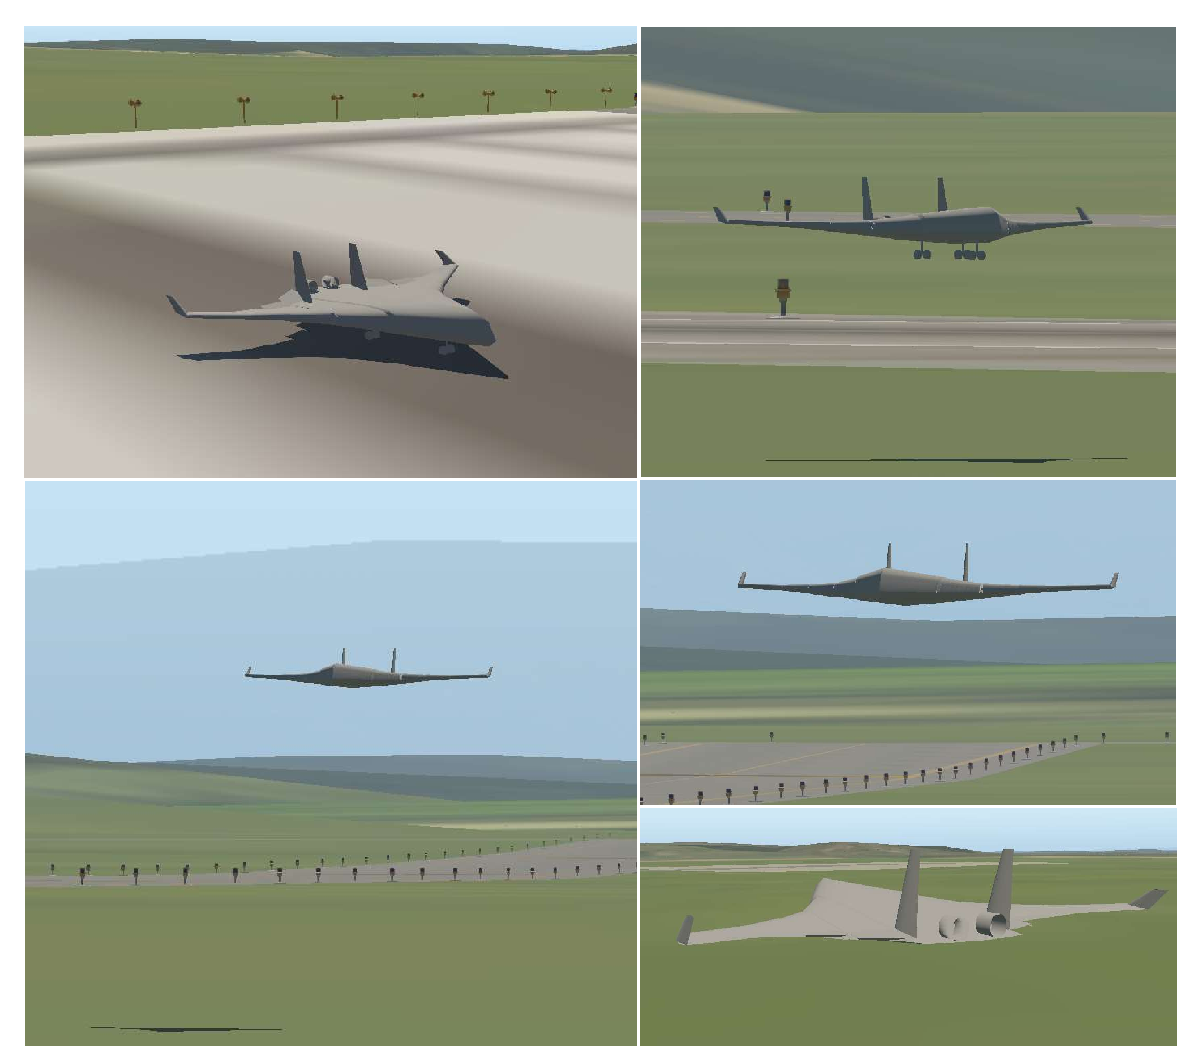
\includegraphics[scale=0.7]{Capitulo3/figs/render ascenso.pdf}
    \caption{EHEKATL BWB simulation images during X-PLANE take-off and ascent}
    \label{render ascenso}
\end{figure}

\textbf{Results Discussions:}
\begin{itemize}
    \item In graph a) EHEKATL BWB navigation is shown in 3D according to altitude, latitude and longitude. For this mission a wing angle is set that approaches zero to maintain a straight and level flight. The pitch angle maintains a value of 1.75$^\circ$ and an engine power of 90$\%$ for a ROC of 2$m/s$.
\begin{figure}[!h]
    \centering
    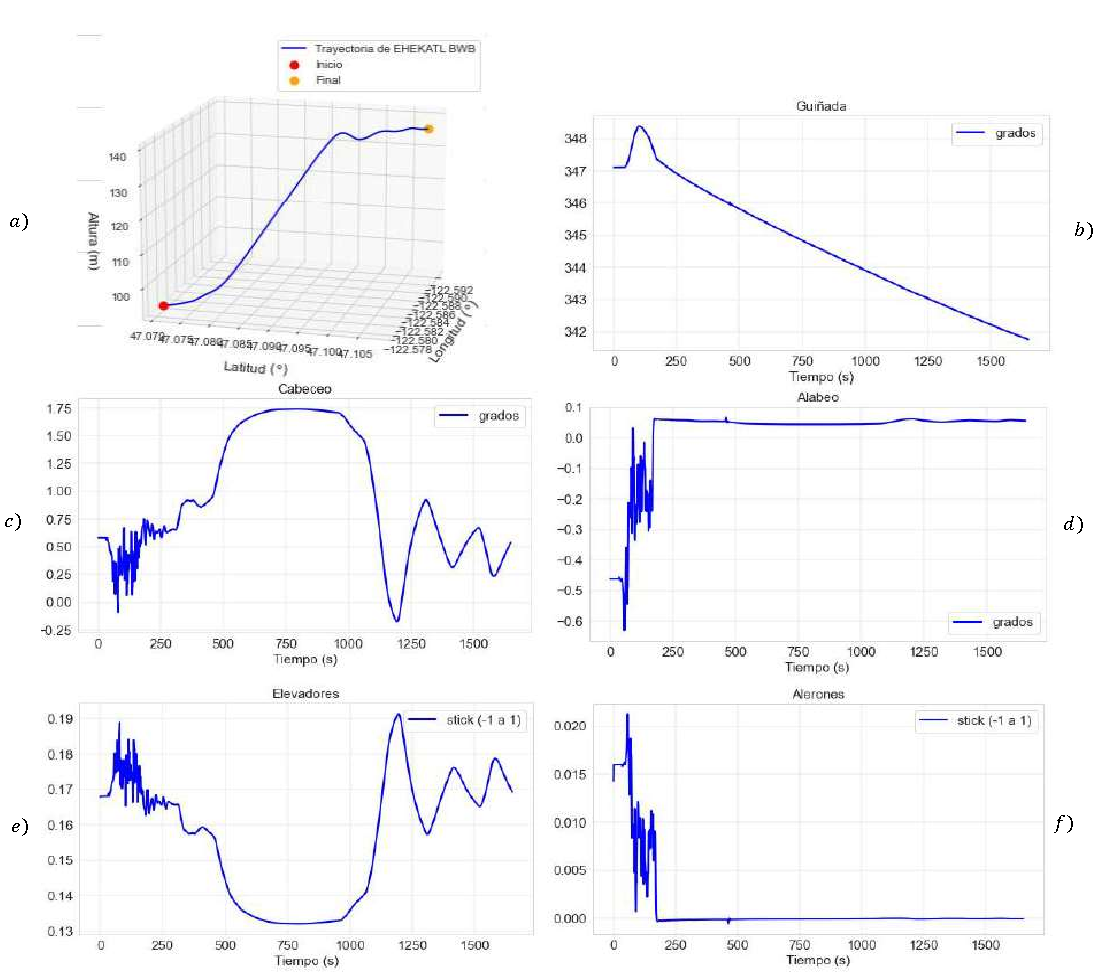
\includegraphics[scale=0.7]{Capitulo3/figs/despegue y ascenso ehekatl 2.pdf}
    \caption{EHEKATL BWB Takeoff and Promotion Mission in the X-PLANE simulator with FCS Bacsktepping}
    \label{Misión de Despegue y Ascenso de EHEKATL BWB en el simulador X-PLANE con FCS Bacsktepping}
\end{figure}
    Once the altitude of 135m is reached, the power of the engines is adjusted to maintain the altitude at constant speed. In graph (b), the yaw in X-PLANE does not refer to the axis $z$ in the body reference system of EHEKATL BWB from an initial inertial condition, but rather at 360$^\circ$ which can be measured with a compass, and according to this coordinates where the nose of EHEKAT BWB points to know the orientation of the direction or direction. Hence the yaw is a navigation tool according to the direction or direction.
    \item Figures (d) and (b) show that at the time of take-off the wings generate a moment in rolling to seek to keep the flight level. This is due to the atmospheric disturbances that occurred during the shooting and take-off. Under such circumstances, the FCS by Backsepping has to control the wings to achieve a response in the orientation of the wing near zero. Such atmospheric peturbations allowed to see the sensitivity of wing-integrated aircraft at low speeds. Once EHEKATL BWB is supported and begins to gain height the value of rolling remains constant.
    \item Finally, in graphs (c) and (e) the pitch response is observed according to the deflection of the lifts. The oscillations that are seen at the beginning of the simulation are due to the fact that the FCS tries to adjust the lifts to achieve the pitch angle of 1.75.$^\circ$ and a constant ROC, however, the speed is very low. During simulations it was observed that EHEKATL BWB begins to generate support from a Mach of 0.04. As time passes and EHEKATL BWB gains altitude, the elevators have a constant value of the stick of 0.125 to maintain the angle of 1.75$^\circ$. It is important to remember that the maximum capacity of the stick is 1 and -1. After the constant ROC of 2$m/s$, try to keep a ROC of 0$m/s$ to maintain a cruise flight at constant altitude. To achieve this mission the power of the engines is adjusted manually. To a power of the engines of 45$\%$, with the same value in the FCS for the pitch orientation, the constant altitude is achieved with some oscillations during the pitching.
    \item Finally, important conclusions are mentioned during the simulation in the phase of take-off and ascent. The values assigned for the FCS by Backstepping were 0 for the orientation in rolling and 6 for the orientation in pitching. These values achieved a satisfactory take-off and ascent to a power of the engines of the $90\%$. When the adjustment was made in the power of the engines it was maintained these same values in the controller. Hence a recommended option arises for the transition of ascent to the cruise flight: once EHEKATL BWB passes from take-off and ascent, it would be necessary to adjust the value of the orientation of the pitching to maintain a flight at constant altitude. During the investigation it was shown that this value can be between 1 and 3 in the orientation of pitch depending on the atmospheric conditions.  
\end{itemize}

\section{Reconnaissance}
The second simulation is dedicated to a reconnaissance mission, see Figures \ref{render reconocimiento} and \ref{Misión de Reconocimiento de EHEKATL BWB en el simulador X-PLANE con FCS Backstepping}. Here, EHEKATL BWB explores its environment using the FCS by Backstepping at a constant rate of turning to the right and looking to keep the attitude in pitch. In the first three turns an engine power is maintained for a ROC of 1$m/s$, then adjusts the engine power to have a negative ROC and achieve descent by maintaining the same values in FCS by Backstepping. Below are the discussions of the simulation results of the Figure \ref{Misión de Reconocimiento de EHEKATL BWB en el simulador X-PLANE con FCS Backstepping}.

\begin{figure}[!h]
    \centering
    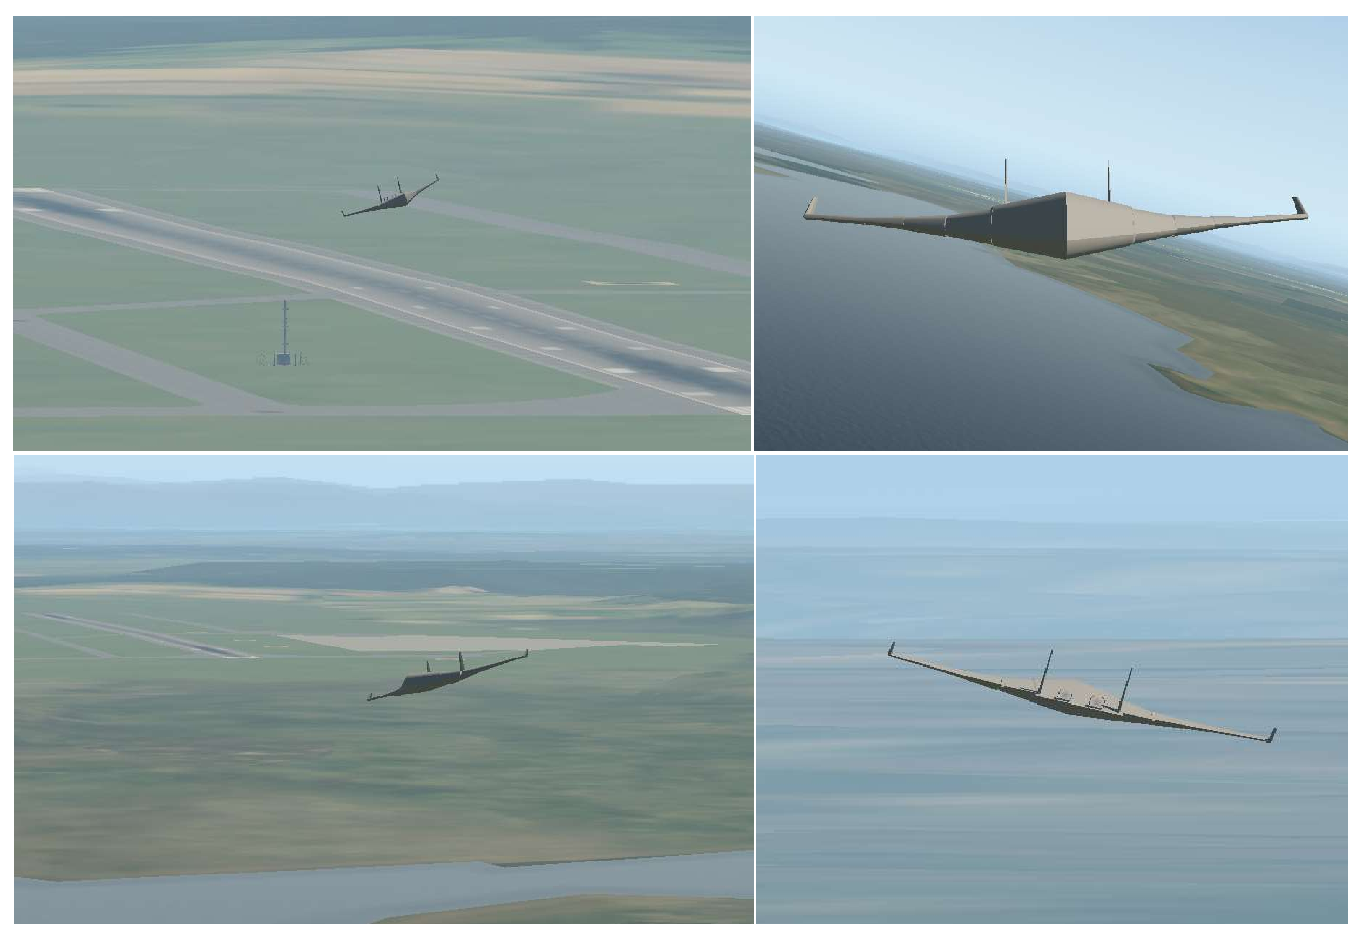
\includegraphics[scale=0.6]{Capitulo3/figs/render reconocimiento.pdf}
    \caption{EHEKATL BWB simulation images during X-PLANE recognition}
    \label{render reconocimiento}
\end{figure}

\textbf{Discussion of the Results:}
\begin{itemize}
    \item Chart a) shows the trajectory of EHEKATL BWB in 3D. It maintains a turn rate to the right and manages to rise its altitude for 3 turns, then descend in three turns.
    \item Chart b) shows the yaw in this constant spin going from 0$^\circ$ to 360$^\circ$ over and over again, during the entire flight mission.
    \item In graph (d) the rate of wing rotation is kept constant with a deflection of the pins of 0.175 which is observed in graph (f), while in graph (c) a variable pitch attitude is observed, and its similar response in graph (e) with the deflection of its lifts.
    \item The values assigned in the FCS by Backstepping are 12 for the roll orientation, 4.5 for the pitch orientation with a ROC of ascent and 0.9 in the pitch orientation with a ROC of descent. The positive value in the FCS for the roll orientation indicates a turn to the right, while a negative value indicates a turn to the left. 
\begin{figure}[!h]
    \centering
    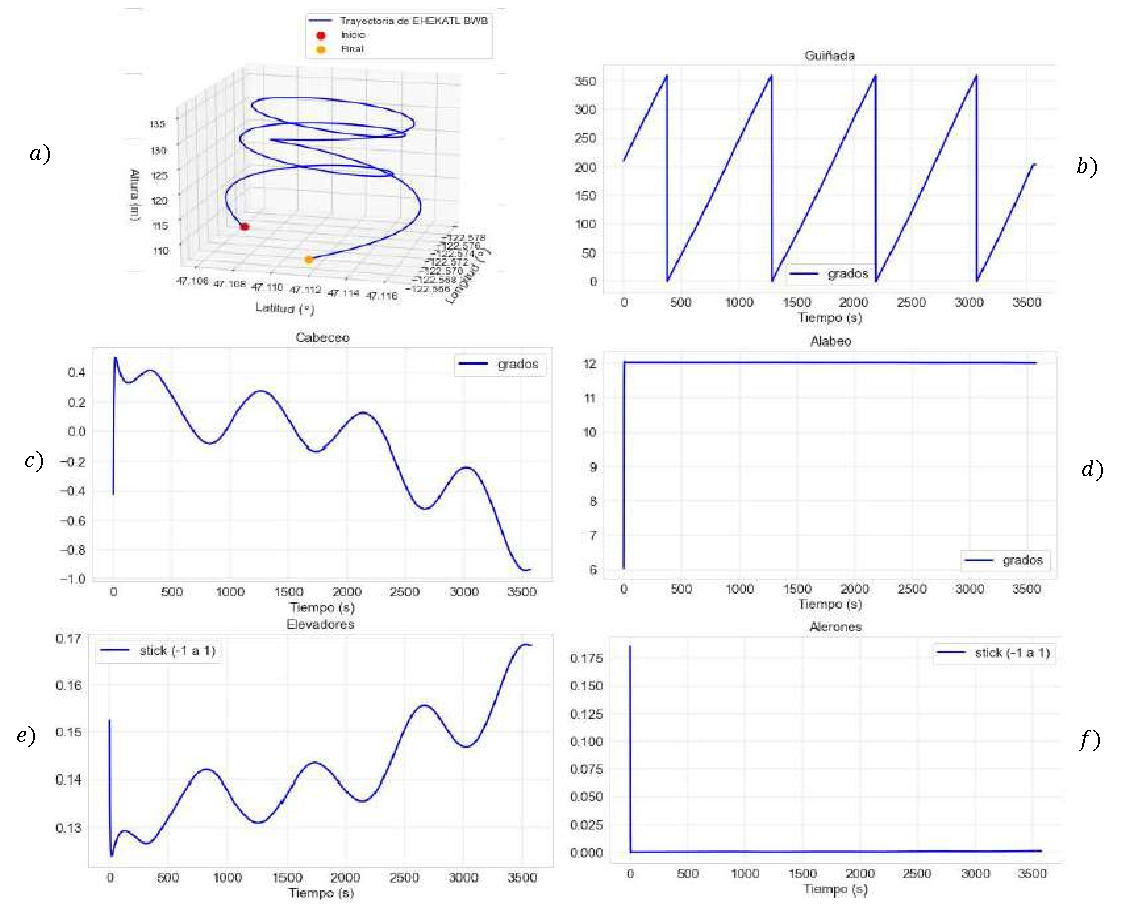
\includegraphics[scale=0.7]{Capitulo3/figs/reconocimiento ehekatl 2.pdf}
    \caption{EHEKATL BWB Recognition Mission in X-PLANE simulator with FCS Backstepping}
    \label{Misión de Reconocimiento de EHEKATL BWB en el simulador X-PLANE con FCS Backstepping}
\end{figure}
\end{itemize}

 
\section{Descent and Landing}

The third and final simulation scenario addresses descent and landing, considered the most critical flight phase, see Figure \ref{render landing} and \ref{Misión de Descenso y Aterrizaje de EHEKATL BWB en el simulador X-PLANE con FCS Backstepping}. Below is the discussion of the results according to the simulation of the Figure \ref{Misión de Descenso y Aterrizaje de EHEKATL BWB en el simulador X-PLANE con FCS Backstepping}. 

\begin{figure}[!t]
    \centering
    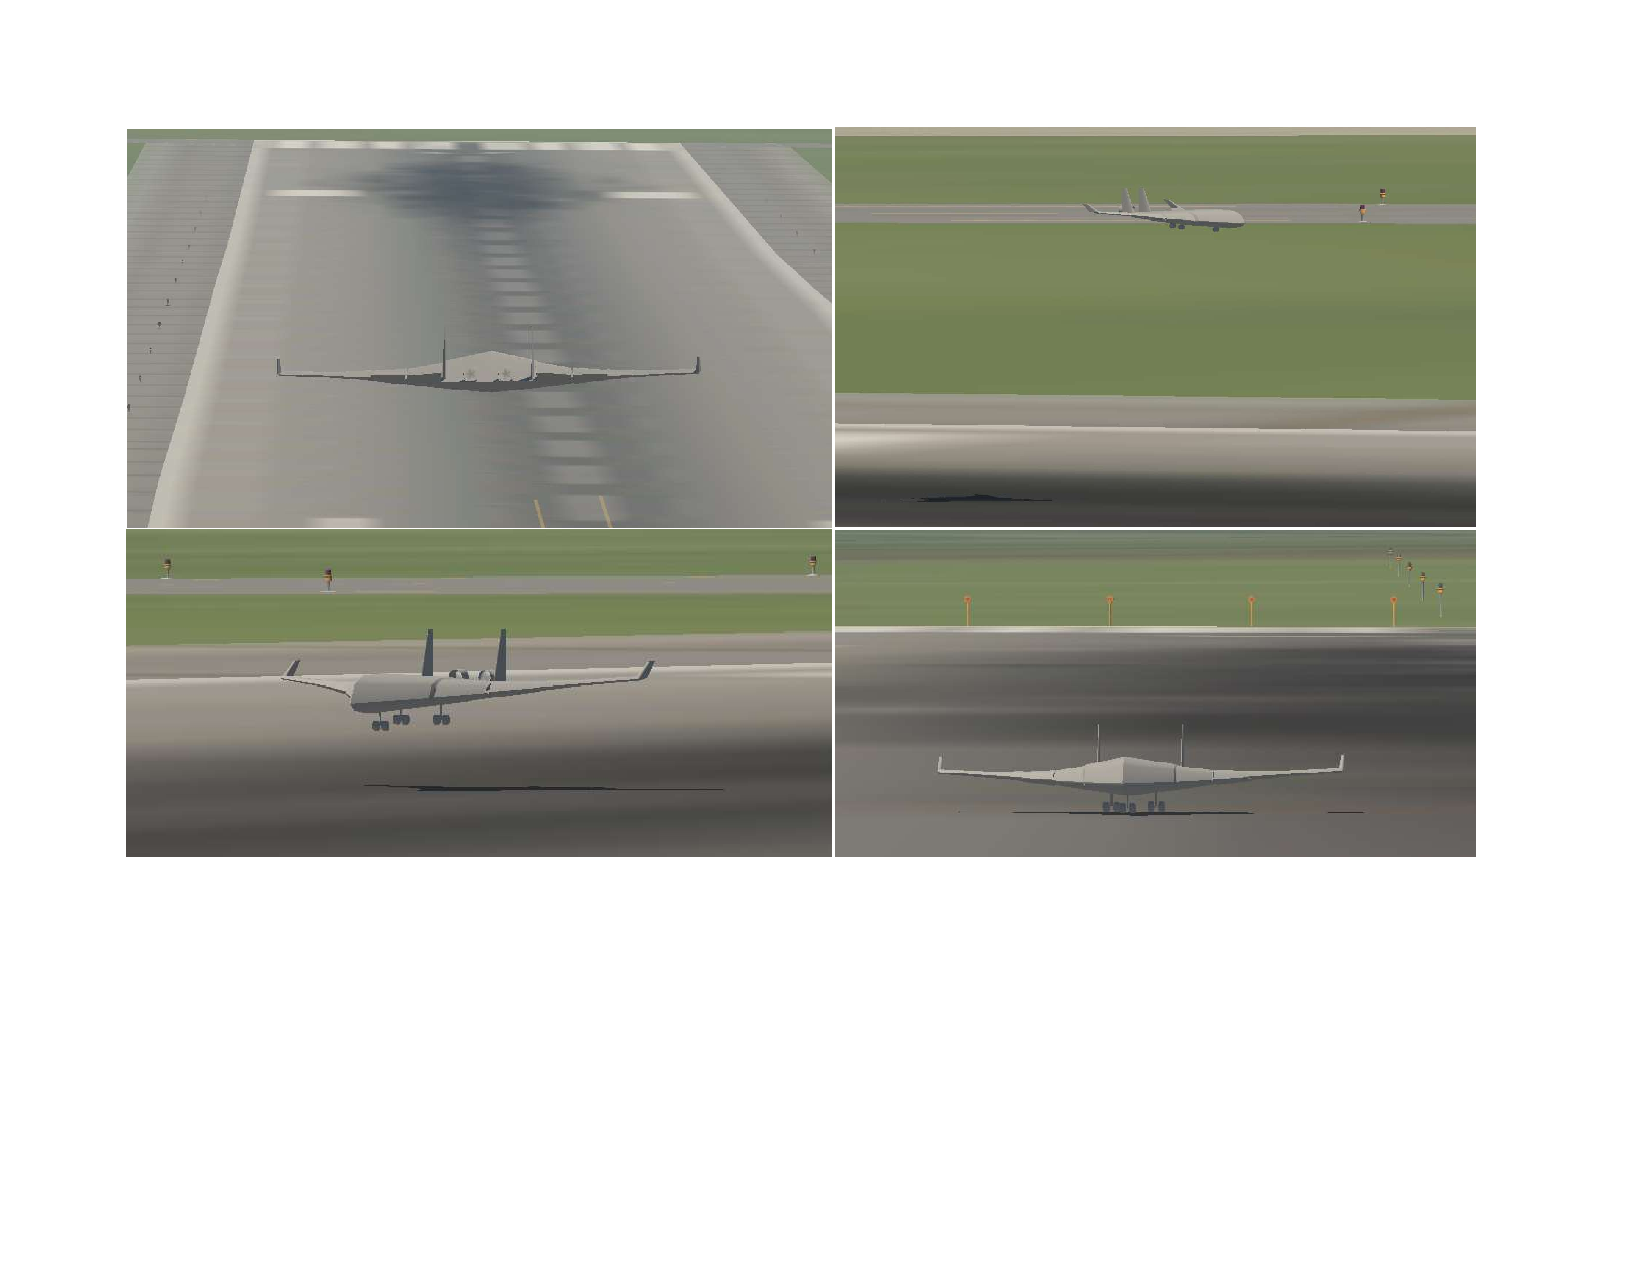
\includegraphics[scale=0.6]{Capitulo3/figs/render aterrizaje_cropped.pdf}
    \caption{EHEKATL BWB simulation images during descent and landing on X-PLANE}
    \label{render landing}
\end{figure}
\begin{figure}[!h]
    \centering
    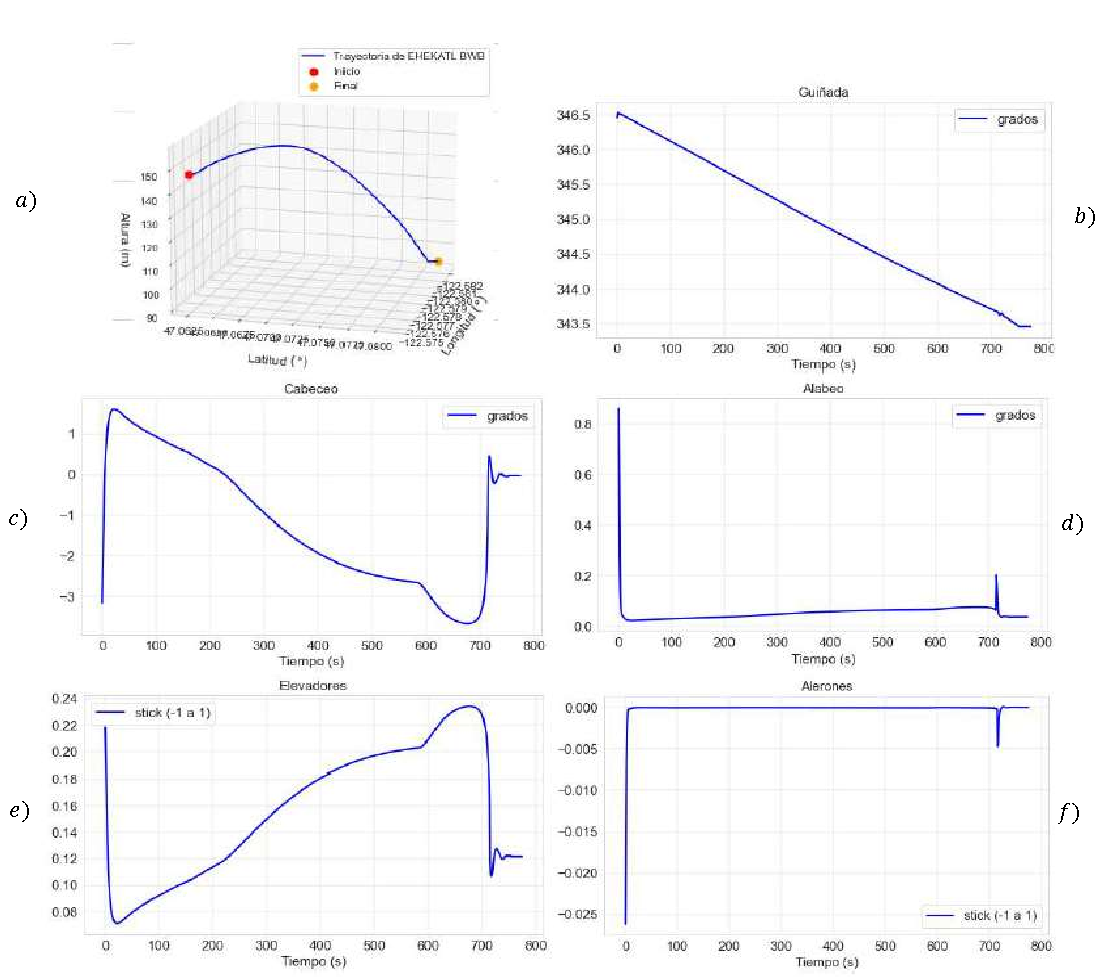
\includegraphics[scale=0.7]{Capitulo3/figs/aterrizaje ehekatl 2.pdf}
    \caption{EHEKATL BWB Descent and Landing Mission in the X-PLANE simulator with FCS Backstepping}
    \label{Misión de Descenso y Aterrizaje de EHEKATL BWB en el simulador X-PLANE con FCS Backstepping}
\end{figure}

\textbf{Results Discussions:}
\begin{itemize}
    \item Chart (a) shows the trajectory of EHEKATL BWB in 3D during descent and landing. To achieve this crucial mission, the FCS was set up by Backstepping with an abbreviated value of 0 and a pitch value of 3. Engine power dropped to 5$\%$, to go down to a Mach speed of between 0.05 and 0.04, which is the speed with which it makes contact on the ground. The parable of descent shows this behavior, where it is seen how the curve is descending, going from a speed of Mach 0.085 on cruise to a speed of descent of 0.05 and touching ground at a speed of 0.04, where the brakes are activated and the aircraft continues to descend its speed until it is still immobile. 
    \item graph b) shows the yaw as to direction or direction, ranging from 346.5 to 343.5.
    \item Figures (d) and (f) show that the ailerons remain constant although before landing they make a small adjustment to achieve ground contact in a straight and level manner. 
    \item In graphs (c) and (e) it is observed that the pitching decreases to achieve the descent from a speed of Mach 0.085 to a speed of Mach 0.04. Before touching the ground the controller manages to raise the nose to make contact with the rear landing gear, then the adjustment is made to descend the nose and make ground contact with the front train.
\end{itemize}

\section{Discussion}  

Conducting X-PLANE flight simulations during the ascent and take-off phase provides a valuable platform for assessing the initial performance of the EHEKATL BWB. Data obtained at this stage are essential to validate the aircraft’s ability to overcome air resistance and achieve a smooth transition to cruise flight.

The reconnaissance phase in X-PLANE flight simulations represents a scenario for assessing stability and manoeuvrability during a sustained turn. 

The descent and landing phase is a crucial stage in the flight cycle of any aircraft. Detailed simulations in X-PLANE during this phase allow to evaluate the ability of the EHEKATL BWB to carry out safe and accurate approach and landing maneuvers in a variety of environmental and air traffic conditions.

Flight simulations in X-PLANE represent an essential component in the validation and refinement of the design of the EHEKATL BWB aircraft. The results obtained from these simulations influence the final design decisions and the configuration of the FCS and navigation on board the aircraft.










